% Generated by Sphinx.
\def\sphinxdocclass{report}
\documentclass[letterpaper,10pt,english]{sphinxmanual}
\usepackage[utf8]{inputenc}
\DeclareUnicodeCharacter{00A0}{\nobreakspace}
\usepackage[T1]{fontenc}
\usepackage{babel}
\usepackage{times}
\usepackage[Bjarne]{fncychap}
\usepackage{longtable}
\usepackage{sphinx}
\usepackage{multirow}


\title{serge Documentation}
\date{July 14, 2012}
\release{0.4}
\author{Paul Paterson}
\newcommand{\sphinxlogo}{}
\renewcommand{\releasename}{Release}
\makeindex

\makeatletter
\def\PYG@reset{\let\PYG@it=\relax \let\PYG@bf=\relax%
    \let\PYG@ul=\relax \let\PYG@tc=\relax%
    \let\PYG@bc=\relax \let\PYG@ff=\relax}
\def\PYG@tok#1{\csname PYG@tok@#1\endcsname}
\def\PYG@toks#1+{\ifx\relax#1\empty\else%
    \PYG@tok{#1}\expandafter\PYG@toks\fi}
\def\PYG@do#1{\PYG@bc{\PYG@tc{\PYG@ul{%
    \PYG@it{\PYG@bf{\PYG@ff{#1}}}}}}}
\def\PYG#1#2{\PYG@reset\PYG@toks#1+\relax+\PYG@do{#2}}

\def\PYG@tok@gd{\def\PYG@tc##1{\textcolor[rgb]{0.63,0.00,0.00}{##1}}}
\def\PYG@tok@gu{\let\PYG@bf=\textbf\def\PYG@tc##1{\textcolor[rgb]{0.50,0.00,0.50}{##1}}}
\def\PYG@tok@gt{\def\PYG@tc##1{\textcolor[rgb]{0.00,0.25,0.82}{##1}}}
\def\PYG@tok@gs{\let\PYG@bf=\textbf}
\def\PYG@tok@gr{\def\PYG@tc##1{\textcolor[rgb]{1.00,0.00,0.00}{##1}}}
\def\PYG@tok@cm{\let\PYG@it=\textit\def\PYG@tc##1{\textcolor[rgb]{0.25,0.50,0.56}{##1}}}
\def\PYG@tok@vg{\def\PYG@tc##1{\textcolor[rgb]{0.73,0.38,0.84}{##1}}}
\def\PYG@tok@m{\def\PYG@tc##1{\textcolor[rgb]{0.13,0.50,0.31}{##1}}}
\def\PYG@tok@mh{\def\PYG@tc##1{\textcolor[rgb]{0.13,0.50,0.31}{##1}}}
\def\PYG@tok@cs{\def\PYG@tc##1{\textcolor[rgb]{0.25,0.50,0.56}{##1}}\def\PYG@bc##1{\colorbox[rgb]{1.00,0.94,0.94}{##1}}}
\def\PYG@tok@ge{\let\PYG@it=\textit}
\def\PYG@tok@vc{\def\PYG@tc##1{\textcolor[rgb]{0.73,0.38,0.84}{##1}}}
\def\PYG@tok@il{\def\PYG@tc##1{\textcolor[rgb]{0.13,0.50,0.31}{##1}}}
\def\PYG@tok@go{\def\PYG@tc##1{\textcolor[rgb]{0.19,0.19,0.19}{##1}}}
\def\PYG@tok@cp{\def\PYG@tc##1{\textcolor[rgb]{0.00,0.44,0.13}{##1}}}
\def\PYG@tok@gi{\def\PYG@tc##1{\textcolor[rgb]{0.00,0.63,0.00}{##1}}}
\def\PYG@tok@gh{\let\PYG@bf=\textbf\def\PYG@tc##1{\textcolor[rgb]{0.00,0.00,0.50}{##1}}}
\def\PYG@tok@ni{\let\PYG@bf=\textbf\def\PYG@tc##1{\textcolor[rgb]{0.84,0.33,0.22}{##1}}}
\def\PYG@tok@nl{\let\PYG@bf=\textbf\def\PYG@tc##1{\textcolor[rgb]{0.00,0.13,0.44}{##1}}}
\def\PYG@tok@nn{\let\PYG@bf=\textbf\def\PYG@tc##1{\textcolor[rgb]{0.05,0.52,0.71}{##1}}}
\def\PYG@tok@no{\def\PYG@tc##1{\textcolor[rgb]{0.38,0.68,0.84}{##1}}}
\def\PYG@tok@na{\def\PYG@tc##1{\textcolor[rgb]{0.25,0.44,0.63}{##1}}}
\def\PYG@tok@nb{\def\PYG@tc##1{\textcolor[rgb]{0.00,0.44,0.13}{##1}}}
\def\PYG@tok@nc{\let\PYG@bf=\textbf\def\PYG@tc##1{\textcolor[rgb]{0.05,0.52,0.71}{##1}}}
\def\PYG@tok@nd{\let\PYG@bf=\textbf\def\PYG@tc##1{\textcolor[rgb]{0.33,0.33,0.33}{##1}}}
\def\PYG@tok@ne{\def\PYG@tc##1{\textcolor[rgb]{0.00,0.44,0.13}{##1}}}
\def\PYG@tok@nf{\def\PYG@tc##1{\textcolor[rgb]{0.02,0.16,0.49}{##1}}}
\def\PYG@tok@si{\let\PYG@it=\textit\def\PYG@tc##1{\textcolor[rgb]{0.44,0.63,0.82}{##1}}}
\def\PYG@tok@s2{\def\PYG@tc##1{\textcolor[rgb]{0.25,0.44,0.63}{##1}}}
\def\PYG@tok@vi{\def\PYG@tc##1{\textcolor[rgb]{0.73,0.38,0.84}{##1}}}
\def\PYG@tok@nt{\let\PYG@bf=\textbf\def\PYG@tc##1{\textcolor[rgb]{0.02,0.16,0.45}{##1}}}
\def\PYG@tok@nv{\def\PYG@tc##1{\textcolor[rgb]{0.73,0.38,0.84}{##1}}}
\def\PYG@tok@s1{\def\PYG@tc##1{\textcolor[rgb]{0.25,0.44,0.63}{##1}}}
\def\PYG@tok@gp{\let\PYG@bf=\textbf\def\PYG@tc##1{\textcolor[rgb]{0.78,0.36,0.04}{##1}}}
\def\PYG@tok@sh{\def\PYG@tc##1{\textcolor[rgb]{0.25,0.44,0.63}{##1}}}
\def\PYG@tok@ow{\let\PYG@bf=\textbf\def\PYG@tc##1{\textcolor[rgb]{0.00,0.44,0.13}{##1}}}
\def\PYG@tok@sx{\def\PYG@tc##1{\textcolor[rgb]{0.78,0.36,0.04}{##1}}}
\def\PYG@tok@bp{\def\PYG@tc##1{\textcolor[rgb]{0.00,0.44,0.13}{##1}}}
\def\PYG@tok@c1{\let\PYG@it=\textit\def\PYG@tc##1{\textcolor[rgb]{0.25,0.50,0.56}{##1}}}
\def\PYG@tok@kc{\let\PYG@bf=\textbf\def\PYG@tc##1{\textcolor[rgb]{0.00,0.44,0.13}{##1}}}
\def\PYG@tok@c{\let\PYG@it=\textit\def\PYG@tc##1{\textcolor[rgb]{0.25,0.50,0.56}{##1}}}
\def\PYG@tok@mf{\def\PYG@tc##1{\textcolor[rgb]{0.13,0.50,0.31}{##1}}}
\def\PYG@tok@err{\def\PYG@bc##1{\fcolorbox[rgb]{1.00,0.00,0.00}{1,1,1}{##1}}}
\def\PYG@tok@kd{\let\PYG@bf=\textbf\def\PYG@tc##1{\textcolor[rgb]{0.00,0.44,0.13}{##1}}}
\def\PYG@tok@ss{\def\PYG@tc##1{\textcolor[rgb]{0.32,0.47,0.09}{##1}}}
\def\PYG@tok@sr{\def\PYG@tc##1{\textcolor[rgb]{0.14,0.33,0.53}{##1}}}
\def\PYG@tok@mo{\def\PYG@tc##1{\textcolor[rgb]{0.13,0.50,0.31}{##1}}}
\def\PYG@tok@mi{\def\PYG@tc##1{\textcolor[rgb]{0.13,0.50,0.31}{##1}}}
\def\PYG@tok@kn{\let\PYG@bf=\textbf\def\PYG@tc##1{\textcolor[rgb]{0.00,0.44,0.13}{##1}}}
\def\PYG@tok@o{\def\PYG@tc##1{\textcolor[rgb]{0.40,0.40,0.40}{##1}}}
\def\PYG@tok@kr{\let\PYG@bf=\textbf\def\PYG@tc##1{\textcolor[rgb]{0.00,0.44,0.13}{##1}}}
\def\PYG@tok@s{\def\PYG@tc##1{\textcolor[rgb]{0.25,0.44,0.63}{##1}}}
\def\PYG@tok@kp{\def\PYG@tc##1{\textcolor[rgb]{0.00,0.44,0.13}{##1}}}
\def\PYG@tok@w{\def\PYG@tc##1{\textcolor[rgb]{0.73,0.73,0.73}{##1}}}
\def\PYG@tok@kt{\def\PYG@tc##1{\textcolor[rgb]{0.56,0.13,0.00}{##1}}}
\def\PYG@tok@sc{\def\PYG@tc##1{\textcolor[rgb]{0.25,0.44,0.63}{##1}}}
\def\PYG@tok@sb{\def\PYG@tc##1{\textcolor[rgb]{0.25,0.44,0.63}{##1}}}
\def\PYG@tok@k{\let\PYG@bf=\textbf\def\PYG@tc##1{\textcolor[rgb]{0.00,0.44,0.13}{##1}}}
\def\PYG@tok@se{\let\PYG@bf=\textbf\def\PYG@tc##1{\textcolor[rgb]{0.25,0.44,0.63}{##1}}}
\def\PYG@tok@sd{\let\PYG@it=\textit\def\PYG@tc##1{\textcolor[rgb]{0.25,0.44,0.63}{##1}}}

\def\PYGZbs{\char`\\}
\def\PYGZus{\char`\_}
\def\PYGZob{\char`\{}
\def\PYGZcb{\char`\}}
\def\PYGZca{\char`\^}
\def\PYGZsh{\char`\#}
\def\PYGZpc{\char`\%}
\def\PYGZdl{\char`\$}
\def\PYGZti{\char`\~}
% for compatibility with earlier versions
\def\PYGZat{@}
\def\PYGZlb{[}
\def\PYGZrb{]}
\makeatother

\begin{document}

\maketitle
\tableofcontents
\phantomsection\label{index::doc}
{\hfill
\includegraphics{logo.png}}



Documentation Overview:


\chapter{Tutorials}
\label{tutorial:tutorials}\label{tutorial:serge-engine-documentation}\label{tutorial::doc}

\section{Tutorial 1: Snake Part 1}
\label{tutorial-1:tutorial-1-snake-part-1}\label{tutorial-1::doc}\setbox0\vbox{
\begin{minipage}{0.95\linewidth}
\textbf{Contents}

\medskip

\begin{itemize}
\item {} 
{\hyperref[tutorial-1:tutorial-1-snake-part-1]{Tutorial 1: Snake Part 1}}
\begin{itemize}
\item {} 
{\hyperref[tutorial-1:introduction]{Introduction}}

\item {} 
{\hyperref[tutorial-1:game]{Game}}

\item {} 
{\hyperref[tutorial-1:engine-overview]{Engine Overview}}

\item {} 
{\hyperref[tutorial-1:setting-things-up-quickly]{Setting Things Up Quickly}}

\item {} 
{\hyperref[tutorial-1:adding-the-snake-s-head]{Adding The Snake's Head}}

\item {} 
{\hyperref[tutorial-1:moving-the-head]{Moving The Head}}

\item {} 
{\hyperref[tutorial-1:interacting-with-the-snake]{Interacting With The Snake}}

\item {} 
{\hyperref[tutorial-1:leaving-a-trail]{Leaving A Trail}}

\item {} 
{\hyperref[tutorial-1:hitting-the-body]{Hitting The Body}}

\item {} 
{\hyperref[tutorial-1:restarting-the-game]{Restarting The Game}}

\item {} 
{\hyperref[tutorial-1:minor-polishing]{Minor Polishing}}

\end{itemize}

\end{itemize}
\end{minipage}}
\begin{center}\setlength{\fboxsep}{5pt}\shadowbox{\box0}\end{center}


\subsection{Introduction}
\label{tutorial-1:introduction}
In this tutorial we will explore some of the basic features of serge. We will
cover {\hyperref[world::doc]{\emph{Worlds}}}, {\hyperref[zone::doc]{\emph{Zones}}}, and {\hyperref[actor::doc]{\emph{Actors}}} using a simple snake game as
an example.

The code for the game is presented as a single file and at each stage the entire code is show. You can simply
copy the code sample into one file and then execute it to run the game. As we add graphics and sounds you will need
to download the game assets. You can download a ZIP file here. This contains the folders and files needed.


\subsection{Game}
\label{tutorial-1:game}
The game we will be building is a simple Snake game. In this game you control
an ever growing snake. You turn the snake head left and right and try to avoid
the head hitting the rest of the body.

We are going to start building the game with simple graphics and then, when
the core game is working we will build in sprites, sounds, and fonts to
make it look more attractive.


\subsection{Engine Overview}
\label{tutorial-1:engine-overview}
The basic structure of a serge game revolves around the main {\hyperref[engine::doc]{\emph{Engine}}}.
The engine runs the game.

Most of what happens in a game, the logic etc, is controlled by various actors.
Actors live in worlds and worlds are divided into zones. Actors have visuals which
are how they appear to the player.

Finally, the engine has a renderer, which handles drawing the actor's visuals to the screen.
Rendering happens on one or more layers. This allows you to control which actors are painted
in front of which, eg to put the player in front of the background.

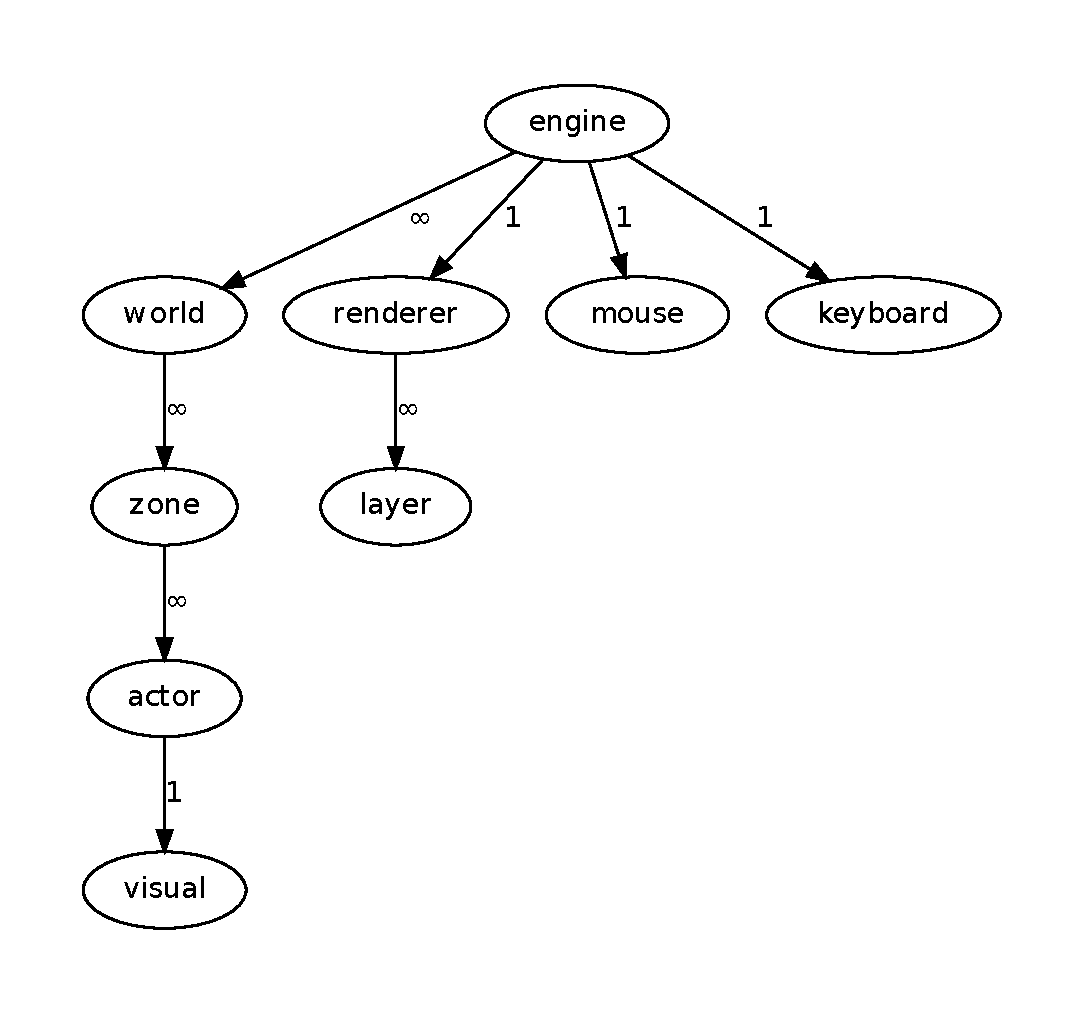
\includegraphics{graphviz-e2e822b8a37c9284baaff76adbf1821ec6eb1438.pdf}


\subsection{Setting Things Up Quickly}
\label{tutorial-1:setting-things-up-quickly}
You have a fair amount of flexibility in how you configure your engine, but for this
example we will use a simple default setup which includes,
\begin{itemize}
\item {} 
a single world, called \emph{lab}, with a single zone

\item {} 
three rendering layers (called \emph{back}, \emph{middle} and \emph{front})

\end{itemize}

Here is the code:

\begin{Verbatim}[commandchars=\\\{\},numbers=left,firstnumber=1,stepnumber=1]
\PYG{k+kn}{import} \PYG{n+nn}{serge.blocks.utils}

\PYG{n}{engine} \PYG{o}{=} \PYG{n}{serge}\PYG{o}{.}\PYG{n}{blocks}\PYG{o}{.}\PYG{n}{utils}\PYG{o}{.}\PYG{n}{getSimpleSetup}\PYG{p}{(}\PYG{l+m+mi}{800}\PYG{p}{,} \PYG{l+m+mi}{600}\PYG{p}{)}
\PYG{n}{engine}\PYG{o}{.}\PYG{n}{run}\PYG{p}{(}\PYG{l+m+mi}{60}\PYG{p}{)}
\end{Verbatim}

When you run this you should see some logging appear in the console and then a blank window
will appear.

The \emph{getSimpleSetup} call returns an engine which will render to a screen of size 800x600. The
call to \emph{engine.run} then runs the engine at 60 frames per second.


\subsection{Adding The Snake's Head}
\label{tutorial-1:adding-the-snake-s-head}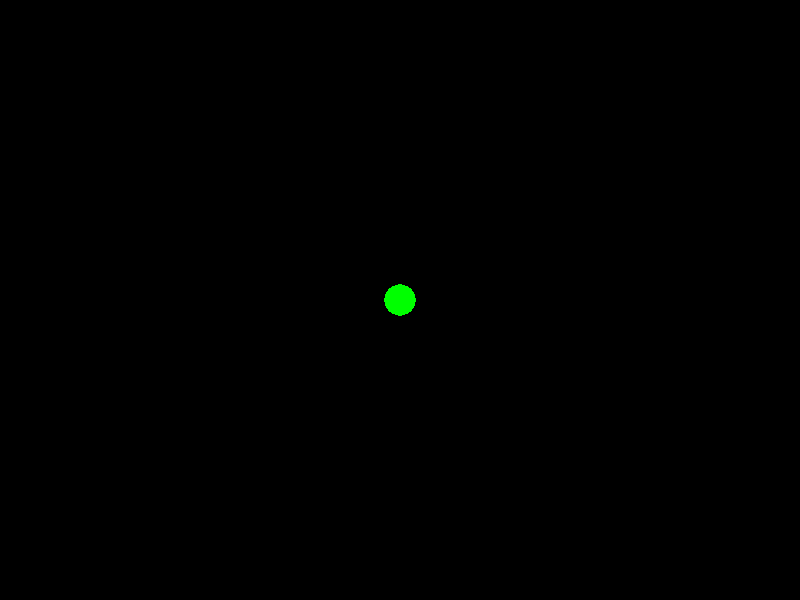
\includegraphics{ss-1-circle.png}
Ok, let's now add the head of the snake. There will be a fail amount of logic associated
with the snake so we normally want to encapsulate this in an actor. To begin with we
will create the head as a simple circle using the following code.

\begin{Verbatim}[commandchars=\\\{\},numbers=left,firstnumber=1,stepnumber=1]
\PYG{k+kn}{import} \PYG{n+nn}{serge.actor}
\PYG{k+kn}{import} \PYG{n+nn}{serge.blocks.visualblocks}
\PYG{k+kn}{import} \PYG{n+nn}{serge.blocks.utils}

\PYG{k}{class} \PYG{n+nc}{Snake}\PYG{p}{(}\PYG{n}{serge}\PYG{o}{.}\PYG{n}{actor}\PYG{o}{.}\PYG{n}{Actor}\PYG{p}{)}\PYG{p}{:}
    \PYG{l+s+sd}{"""Represents the snake"""}

    \PYG{k}{def} \PYG{n+nf}{\PYGZus{}\PYGZus{}init\PYGZus{}\PYGZus{}}\PYG{p}{(}\PYG{n+nb+bp}{self}\PYG{p}{)}\PYG{p}{:}
        \PYG{l+s+sd}{"""Initialise the snake"""}
        \PYG{n+nb}{super}\PYG{p}{(}\PYG{n}{Snake}\PYG{p}{,} \PYG{n+nb+bp}{self}\PYG{p}{)}\PYG{o}{.}\PYG{n}{\PYGZus{}\PYGZus{}init\PYGZus{}\PYGZus{}}\PYG{p}{(}\PYG{l+s}{'}\PYG{l+s}{snake}\PYG{l+s}{'}\PYG{p}{,} \PYG{l+s}{'}\PYG{l+s}{snake-head}\PYG{l+s}{'}\PYG{p}{)}
        \PYG{n+nb+bp}{self}\PYG{o}{.}\PYG{n}{visual} \PYG{o}{=} \PYG{n}{serge}\PYG{o}{.}\PYG{n}{blocks}\PYG{o}{.}\PYG{n}{visualblocks}\PYG{o}{.}\PYG{n}{Circle}\PYG{p}{(}\PYG{l+m+mi}{16}\PYG{p}{,} \PYG{p}{(}\PYG{l+m+mi}{0}\PYG{p}{,}\PYG{l+m+mi}{255}\PYG{p}{,}\PYG{l+m+mi}{0}\PYG{p}{)}\PYG{p}{)}
        \PYG{n+nb+bp}{self}\PYG{o}{.}\PYG{n}{setLayerName}\PYG{p}{(}\PYG{l+s}{'}\PYG{l+s}{middle}\PYG{l+s}{'}\PYG{p}{)}

\PYG{c}{\PYGZsh{} Create the engine}
\PYG{n}{engine} \PYG{o}{=} \PYG{n}{serge}\PYG{o}{.}\PYG{n}{blocks}\PYG{o}{.}\PYG{n}{utils}\PYG{o}{.}\PYG{n}{getSimpleSetup}\PYG{p}{(}\PYG{l+m+mi}{800}\PYG{p}{,} \PYG{l+m+mi}{600}\PYG{p}{)}
\PYG{n}{world} \PYG{o}{=} \PYG{n}{engine}\PYG{o}{.}\PYG{n}{getWorld}\PYG{p}{(}\PYG{l+s}{'}\PYG{l+s}{lab}\PYG{l+s}{'}\PYG{p}{)}

\PYG{c}{\PYGZsh{} Create the snake}
\PYG{n}{snake} \PYG{o}{=} \PYG{n}{Snake}\PYG{p}{(}\PYG{p}{)}
\PYG{n}{world}\PYG{o}{.}\PYG{n}{addActor}\PYG{p}{(}\PYG{n}{snake}\PYG{p}{)}
\PYG{n}{snake}\PYG{o}{.}\PYG{n}{moveTo}\PYG{p}{(}\PYG{l+m+mi}{400}\PYG{p}{,} \PYG{l+m+mi}{300}\PYG{p}{)}

\PYG{c}{\PYGZsh{} Run the game}
\PYG{n}{engine}\PYG{o}{.}\PYG{n}{run}\PYG{p}{(}\PYG{l+m+mi}{60}\PYG{p}{)}
\end{Verbatim}

When you run this you should see a green circle in the middle of the screen. This is the snakes
head. The graphic comes from the line:

\begin{Verbatim}[commandchars=\\\{\}]
\PYG{n+nb+bp}{self}\PYG{o}{.}\PYG{n}{visual} \PYG{o}{=} \PYG{n}{serge}\PYG{o}{.}\PYG{n}{blocks}\PYG{o}{.}\PYG{n}{visualblocks}\PYG{o}{.}\PYG{n}{Circle}\PYG{p}{(}\PYG{l+m+mi}{16}\PYG{p}{,} \PYG{p}{(}\PYG{l+m+mi}{0}\PYG{p}{,}\PYG{l+m+mi}{255}\PYG{p}{,}\PYG{l+m+mi}{0}\PYG{p}{)}\PYG{p}{)}
\end{Verbatim}

This sets the visual representation of the actor to be a green circle with a radius of 16 pixels.
Later on we will replace this with a sprite but for now let's keep it simple.


\subsection{Moving The Head}
\label{tutorial-1:moving-the-head}
Now it is time to move the snake's head.

The engine will call the \emph{updateActor} method on an actors in the currently active world every
timestep. This is the normal way that we perform any game logic and so we will use it to move
the snake.

We need to give the snake a certain direction, which we set up in the \emph{\_\_init\_\_} method. There
is a \emph{block} that we can make use of for cardinal directions.

\begin{Verbatim}[commandchars=\\\{\},numbers=left,firstnumber=1,stepnumber=1]
\PYG{k+kn}{import} \PYG{n+nn}{serge.actor}
\PYG{k+kn}{import} \PYG{n+nn}{serge.blocks.visualblocks}
\PYG{k+kn}{import} \PYG{n+nn}{serge.blocks.utils}
\PYG{k+kn}{import} \PYG{n+nn}{serge.blocks.directions}

\PYG{k}{class} \PYG{n+nc}{Snake}\PYG{p}{(}\PYG{n}{serge}\PYG{o}{.}\PYG{n}{actor}\PYG{o}{.}\PYG{n}{Actor}\PYG{p}{)}\PYG{p}{:}
    \PYG{l+s+sd}{"""Represents the snake"""}

    \PYG{k}{def} \PYG{n+nf}{\PYGZus{}\PYGZus{}init\PYGZus{}\PYGZus{}}\PYG{p}{(}\PYG{n+nb+bp}{self}\PYG{p}{)}\PYG{p}{:}
        \PYG{l+s+sd}{"""Initialise the snake"""}
        \PYG{n+nb}{super}\PYG{p}{(}\PYG{n}{Snake}\PYG{p}{,} \PYG{n+nb+bp}{self}\PYG{p}{)}\PYG{o}{.}\PYG{n}{\PYGZus{}\PYGZus{}init\PYGZus{}\PYGZus{}}\PYG{p}{(}\PYG{l+s}{'}\PYG{l+s}{snake}\PYG{l+s}{'}\PYG{p}{,} \PYG{l+s}{'}\PYG{l+s}{snake-head}\PYG{l+s}{'}\PYG{p}{)}
        \PYG{n+nb+bp}{self}\PYG{o}{.}\PYG{n}{visual} \PYG{o}{=} \PYG{n}{serge}\PYG{o}{.}\PYG{n}{blocks}\PYG{o}{.}\PYG{n}{visualblocks}\PYG{o}{.}\PYG{n}{Circle}\PYG{p}{(}\PYG{l+m+mi}{16}\PYG{p}{,} \PYG{p}{(}\PYG{l+m+mi}{0}\PYG{p}{,}\PYG{l+m+mi}{255}\PYG{p}{,}\PYG{l+m+mi}{0}\PYG{p}{)}\PYG{p}{)}
        \PYG{n+nb+bp}{self}\PYG{o}{.}\PYG{n}{setLayerName}\PYG{p}{(}\PYG{l+s}{'}\PYG{l+s}{middle}\PYG{l+s}{'}\PYG{p}{)}
        \PYG{n+nb+bp}{self}\PYG{o}{.}\PYG{n}{current\PYGZus{}direction} \PYG{o}{=} \PYG{n}{serge}\PYG{o}{.}\PYG{n}{blocks}\PYG{o}{.}\PYG{n}{directions}\PYG{o}{.}\PYG{n}{N}

    \PYG{k}{def} \PYG{n+nf}{updateActor}\PYG{p}{(}\PYG{n+nb+bp}{self}\PYG{p}{,} \PYG{n}{interval}\PYG{p}{,} \PYG{n}{world}\PYG{p}{)}\PYG{p}{:}
        \PYG{l+s+sd}{"""Update the snake"""}
        \PYG{n+nb}{super}\PYG{p}{(}\PYG{n}{Snake}\PYG{p}{,} \PYG{n+nb+bp}{self}\PYG{p}{)}\PYG{o}{.}\PYG{n}{updateActor}\PYG{p}{(}\PYG{n}{interval}\PYG{p}{,} \PYG{n}{world}\PYG{p}{)}
        \PYG{c}{\PYGZsh{}}
        \PYG{n}{offset} \PYG{o}{=} \PYG{l+m+mi}{5}\PYG{o}{*}\PYG{n}{serge}\PYG{o}{.}\PYG{n}{blocks}\PYG{o}{.}\PYG{n}{directions}\PYG{o}{.}\PYG{n}{getVectorFromCardinal}\PYG{p}{(}\PYG{n+nb+bp}{self}\PYG{o}{.}\PYG{n}{current\PYGZus{}direction}\PYG{p}{)}
        \PYG{n+nb+bp}{self}\PYG{o}{.}\PYG{n}{move}\PYG{p}{(}\PYG{o}{*}\PYG{n}{offset}\PYG{p}{)}

\PYG{c}{\PYGZsh{} Create the engine}
\PYG{n}{engine} \PYG{o}{=} \PYG{n}{serge}\PYG{o}{.}\PYG{n}{blocks}\PYG{o}{.}\PYG{n}{utils}\PYG{o}{.}\PYG{n}{getSimpleSetup}\PYG{p}{(}\PYG{l+m+mi}{800}\PYG{p}{,} \PYG{l+m+mi}{600}\PYG{p}{)}
\PYG{n}{world} \PYG{o}{=} \PYG{n}{engine}\PYG{o}{.}\PYG{n}{getWorld}\PYG{p}{(}\PYG{l+s}{'}\PYG{l+s}{lab}\PYG{l+s}{'}\PYG{p}{)}

\PYG{c}{\PYGZsh{} Create the snake}
\PYG{n}{snake} \PYG{o}{=} \PYG{n}{Snake}\PYG{p}{(}\PYG{p}{)}
\PYG{n}{world}\PYG{o}{.}\PYG{n}{addActor}\PYG{p}{(}\PYG{n}{snake}\PYG{p}{)}
\PYG{n}{snake}\PYG{o}{.}\PYG{n}{moveTo}\PYG{p}{(}\PYG{l+m+mi}{400}\PYG{p}{,} \PYG{l+m+mi}{300}\PYG{p}{)}

\PYG{c}{\PYGZsh{} Run the game}
\PYG{n}{engine}\PYG{o}{.}\PYG{n}{run}\PYG{p}{(}\PYG{l+m+mi}{60}\PYG{p}{)}
\end{Verbatim}

Now the snake's head should gradually move up the screen. This is going \emph{north} because we
chose this as the current direction in the \emph{\_\_init\_\_} method. The \emph{getVectorFromCardinal} function
returns a \emph{Vec2d} so we can multiply it by any constant to create the right length. You can
experiment with the number 5 to adjust the difficulty of the game.

\textbf{Note} Always remember to call the base class methods (ie using \emph{super}) for methods like \emph{updateActor}.


\subsection{Interacting With The Snake}
\label{tutorial-1:interacting-with-the-snake}
So far the snake is just going forward with no input from the user. Let's now allow the user to
move the head around. We do this by looking for keyboard input.

The engine has a keyboard object and we can use this to check. Note that for efficiency it is
best to get hold of the keyboard object and anything else you may need in the \emph{addedToWorld} method
of an actor. This method is called just after the actor is added to the world and is a great
place to do initialisation. It is usually better to do things here rather than in the \emph{\_\_init\_\_} method
because at \emph{\_\_init\_\_} you do not know anything about the world you are in.

\begin{Verbatim}[commandchars=\\\{\},numbers=left,firstnumber=1,stepnumber=1]
\PYG{k+kn}{import} \PYG{n+nn}{pygame}

\PYG{k+kn}{import} \PYG{n+nn}{serge.engine}
\PYG{k+kn}{import} \PYG{n+nn}{serge.actor}
\PYG{k+kn}{import} \PYG{n+nn}{serge.blocks.visualblocks}
\PYG{k+kn}{import} \PYG{n+nn}{serge.blocks.utils}
\PYG{k+kn}{import} \PYG{n+nn}{serge.blocks.directions}

\PYG{k}{class} \PYG{n+nc}{Snake}\PYG{p}{(}\PYG{n}{serge}\PYG{o}{.}\PYG{n}{actor}\PYG{o}{.}\PYG{n}{Actor}\PYG{p}{)}\PYG{p}{:}
    \PYG{l+s+sd}{"""Represents the snake"""}

    \PYG{k}{def} \PYG{n+nf}{\PYGZus{}\PYGZus{}init\PYGZus{}\PYGZus{}}\PYG{p}{(}\PYG{n+nb+bp}{self}\PYG{p}{)}\PYG{p}{:}
        \PYG{l+s+sd}{"""Initialise the snake"""}
        \PYG{n+nb}{super}\PYG{p}{(}\PYG{n}{Snake}\PYG{p}{,} \PYG{n+nb+bp}{self}\PYG{p}{)}\PYG{o}{.}\PYG{n}{\PYGZus{}\PYGZus{}init\PYGZus{}\PYGZus{}}\PYG{p}{(}\PYG{l+s}{'}\PYG{l+s}{snake}\PYG{l+s}{'}\PYG{p}{,} \PYG{l+s}{'}\PYG{l+s}{snake-head}\PYG{l+s}{'}\PYG{p}{)}
        \PYG{n+nb+bp}{self}\PYG{o}{.}\PYG{n}{visual} \PYG{o}{=} \PYG{n}{serge}\PYG{o}{.}\PYG{n}{blocks}\PYG{o}{.}\PYG{n}{visualblocks}\PYG{o}{.}\PYG{n}{Circle}\PYG{p}{(}\PYG{l+m+mi}{16}\PYG{p}{,} \PYG{p}{(}\PYG{l+m+mi}{0}\PYG{p}{,}\PYG{l+m+mi}{255}\PYG{p}{,}\PYG{l+m+mi}{0}\PYG{p}{)}\PYG{p}{)}
        \PYG{n+nb+bp}{self}\PYG{o}{.}\PYG{n}{setLayerName}\PYG{p}{(}\PYG{l+s}{'}\PYG{l+s}{middle}\PYG{l+s}{'}\PYG{p}{)}
        \PYG{n+nb+bp}{self}\PYG{o}{.}\PYG{n}{current\PYGZus{}direction} \PYG{o}{=} \PYG{n}{serge}\PYG{o}{.}\PYG{n}{blocks}\PYG{o}{.}\PYG{n}{directions}\PYG{o}{.}\PYG{n}{N}

    \PYG{k}{def} \PYG{n+nf}{addedToWorld}\PYG{p}{(}\PYG{n+nb+bp}{self}\PYG{p}{,} \PYG{n}{world}\PYG{p}{)}\PYG{p}{:}
        \PYG{l+s+sd}{"""The snake was added to the world"""}
        \PYG{n+nb}{super}\PYG{p}{(}\PYG{n}{Snake}\PYG{p}{,} \PYG{n+nb+bp}{self}\PYG{p}{)}\PYG{o}{.}\PYG{n}{addedToWorld}\PYG{p}{(}\PYG{n}{world}\PYG{p}{)}
        \PYG{c}{\PYGZsh{}}
        \PYG{n+nb+bp}{self}\PYG{o}{.}\PYG{n}{keyboard} \PYG{o}{=} \PYG{n}{serge}\PYG{o}{.}\PYG{n}{engine}\PYG{o}{.}\PYG{n}{CurrentEngine}\PYG{p}{(}\PYG{p}{)}\PYG{o}{.}\PYG{n}{getKeyboard}\PYG{p}{(}\PYG{p}{)}

    \PYG{k}{def} \PYG{n+nf}{updateActor}\PYG{p}{(}\PYG{n+nb+bp}{self}\PYG{p}{,} \PYG{n}{interval}\PYG{p}{,} \PYG{n}{world}\PYG{p}{)}\PYG{p}{:}
        \PYG{l+s+sd}{"""Update the snake"""}
        \PYG{n+nb}{super}\PYG{p}{(}\PYG{n}{Snake}\PYG{p}{,} \PYG{n+nb+bp}{self}\PYG{p}{)}\PYG{o}{.}\PYG{n}{updateActor}\PYG{p}{(}\PYG{n}{interval}\PYG{p}{,} \PYG{n}{world}\PYG{p}{)}
        \PYG{c}{\PYGZsh{}}
        \PYG{c}{\PYGZsh{} Move the head}
        \PYG{k}{if} \PYG{n+nb+bp}{self}\PYG{o}{.}\PYG{n}{keyboard}\PYG{o}{.}\PYG{n}{isClicked}\PYG{p}{(}\PYG{n}{pygame}\PYG{o}{.}\PYG{n}{K\PYGZus{}LEFT}\PYG{p}{)}\PYG{p}{:}
            \PYG{n}{rotation} \PYG{o}{=} \PYG{o}{+}\PYG{l+m+mi}{90}
        \PYG{k}{elif} \PYG{n+nb+bp}{self}\PYG{o}{.}\PYG{n}{keyboard}\PYG{o}{.}\PYG{n}{isClicked}\PYG{p}{(}\PYG{n}{pygame}\PYG{o}{.}\PYG{n}{K\PYGZus{}RIGHT}\PYG{p}{)}\PYG{p}{:}
            \PYG{n}{rotation} \PYG{o}{=} \PYG{o}{-}\PYG{l+m+mi}{90}
        \PYG{k}{else}\PYG{p}{:}
            \PYG{n}{rotation} \PYG{o}{=} \PYG{l+m+mi}{0}
        \PYG{c}{\PYGZsh{}}
        \PYG{c}{\PYGZsh{} Change direction}
        \PYG{k}{if} \PYG{n}{rotation}\PYG{p}{:}
            \PYG{n}{current\PYGZus{}angle} \PYG{o}{=} \PYG{n}{serge}\PYG{o}{.}\PYG{n}{blocks}\PYG{o}{.}\PYG{n}{directions}\PYG{o}{.}\PYG{n}{getAngleFromCardinal}\PYG{p}{(}\PYG{n+nb+bp}{self}\PYG{o}{.}\PYG{n}{current\PYGZus{}direction}\PYG{p}{)}
            \PYG{n+nb+bp}{self}\PYG{o}{.}\PYG{n}{current\PYGZus{}direction} \PYG{o}{=} \PYG{n}{serge}\PYG{o}{.}\PYG{n}{blocks}\PYG{o}{.}\PYG{n}{directions}\PYG{o}{.}\PYG{n}{getCardinalFromAngle}\PYG{p}{(}\PYG{n}{current\PYGZus{}angle}\PYG{o}{+}\PYG{n}{rotation}\PYG{p}{)}
        \PYG{c}{\PYGZsh{}}
        \PYG{c}{\PYGZsh{} Move}
        \PYG{n}{offset} \PYG{o}{=} \PYG{l+m+mi}{5}\PYG{o}{*}\PYG{n}{serge}\PYG{o}{.}\PYG{n}{blocks}\PYG{o}{.}\PYG{n}{directions}\PYG{o}{.}\PYG{n}{getVectorFromCardinal}\PYG{p}{(}\PYG{n+nb+bp}{self}\PYG{o}{.}\PYG{n}{current\PYGZus{}direction}\PYG{p}{)}
        \PYG{n+nb+bp}{self}\PYG{o}{.}\PYG{n}{move}\PYG{p}{(}\PYG{o}{*}\PYG{n}{offset}\PYG{p}{)}

\PYG{c}{\PYGZsh{} Create the engine}
\PYG{n}{engine} \PYG{o}{=} \PYG{n}{serge}\PYG{o}{.}\PYG{n}{blocks}\PYG{o}{.}\PYG{n}{utils}\PYG{o}{.}\PYG{n}{getSimpleSetup}\PYG{p}{(}\PYG{l+m+mi}{800}\PYG{p}{,} \PYG{l+m+mi}{600}\PYG{p}{)}
\PYG{n}{world} \PYG{o}{=} \PYG{n}{engine}\PYG{o}{.}\PYG{n}{getWorld}\PYG{p}{(}\PYG{l+s}{'}\PYG{l+s}{lab}\PYG{l+s}{'}\PYG{p}{)}

\PYG{c}{\PYGZsh{} Create the snake}
\PYG{n}{snake} \PYG{o}{=} \PYG{n}{Snake}\PYG{p}{(}\PYG{p}{)}
\PYG{n}{world}\PYG{o}{.}\PYG{n}{addActor}\PYG{p}{(}\PYG{n}{snake}\PYG{p}{)}
\PYG{n}{snake}\PYG{o}{.}\PYG{n}{moveTo}\PYG{p}{(}\PYG{l+m+mi}{400}\PYG{p}{,} \PYG{l+m+mi}{300}\PYG{p}{)}

\PYG{c}{\PYGZsh{} Run the game}
\PYG{n}{engine}\PYG{o}{.}\PYG{n}{run}\PYG{p}{(}\PYG{l+m+mi}{60}\PYG{p}{)}
\end{Verbatim}

You should now be able to direct the snake's head using the left and right arrow keys.
Notice that we use the \emph{isClicked} method of the keyboard. This means that the user has
to press and release the key before we will turn the snake. We will see later that
we can use the \emph{isDown} to create a different feel to the game.


\subsection{Leaving A Trail}
\label{tutorial-1:leaving-a-trail}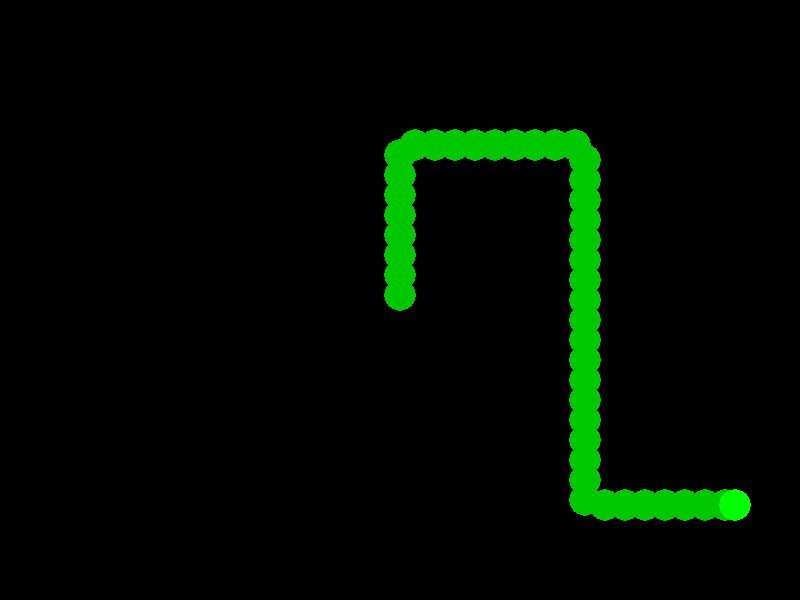
\includegraphics{ss-1-tail.png}
So far the snake is just a head. Let's add a body to it now.

The body of the snake will be made up of a series of segments. We should lay a new
segment down each time we have moved a certain distance. However, we cannot just count
up how far the head has gone since the player may change direction at any time.

So the algorithm is:
\begin{itemize}
\item {} 
Add a new segment to begin with

\item {} 
Each iteration check if adding a new segment would overlap the last

\item {} 
If it overlaps do nothing

\item {} 
It if doesn't overlap then add it

\end{itemize}

Let's look at the code.

\begin{Verbatim}[commandchars=\\\{\},numbers=left,firstnumber=1,stepnumber=1]
\PYG{k+kn}{import} \PYG{n+nn}{pygame}

\PYG{k+kn}{import} \PYG{n+nn}{serge.engine}
\PYG{k+kn}{import} \PYG{n+nn}{serge.actor}
\PYG{k+kn}{import} \PYG{n+nn}{serge.blocks.visualblocks}
\PYG{k+kn}{import} \PYG{n+nn}{serge.blocks.utils}
\PYG{k+kn}{import} \PYG{n+nn}{serge.blocks.directions}

\PYG{k}{class} \PYG{n+nc}{Snake}\PYG{p}{(}\PYG{n}{serge}\PYG{o}{.}\PYG{n}{actor}\PYG{o}{.}\PYG{n}{CompositeActor}\PYG{p}{)}\PYG{p}{:}
    \PYG{l+s+sd}{"""Represents the snake"""}

    \PYG{k}{def} \PYG{n+nf}{\PYGZus{}\PYGZus{}init\PYGZus{}\PYGZus{}}\PYG{p}{(}\PYG{n+nb+bp}{self}\PYG{p}{)}\PYG{p}{:}
        \PYG{l+s+sd}{"""Initialise the snake"""}
        \PYG{n+nb}{super}\PYG{p}{(}\PYG{n}{Snake}\PYG{p}{,} \PYG{n+nb+bp}{self}\PYG{p}{)}\PYG{o}{.}\PYG{n}{\PYGZus{}\PYGZus{}init\PYGZus{}\PYGZus{}}\PYG{p}{(}\PYG{l+s}{'}\PYG{l+s}{snake}\PYG{l+s}{'}\PYG{p}{,} \PYG{l+s}{'}\PYG{l+s}{snake-head}\PYG{l+s}{'}\PYG{p}{)}
        \PYG{n+nb+bp}{self}\PYG{o}{.}\PYG{n}{visual} \PYG{o}{=} \PYG{n}{serge}\PYG{o}{.}\PYG{n}{blocks}\PYG{o}{.}\PYG{n}{visualblocks}\PYG{o}{.}\PYG{n}{Circle}\PYG{p}{(}\PYG{l+m+mi}{16}\PYG{p}{,} \PYG{p}{(}\PYG{l+m+mi}{0}\PYG{p}{,}\PYG{l+m+mi}{255}\PYG{p}{,}\PYG{l+m+mi}{0}\PYG{p}{)}\PYG{p}{)}
        \PYG{n+nb+bp}{self}\PYG{o}{.}\PYG{n}{setLayerName}\PYG{p}{(}\PYG{l+s}{'}\PYG{l+s}{middle}\PYG{l+s}{'}\PYG{p}{)}
        \PYG{n+nb+bp}{self}\PYG{o}{.}\PYG{n}{current\PYGZus{}direction} \PYG{o}{=} \PYG{n}{serge}\PYG{o}{.}\PYG{n}{blocks}\PYG{o}{.}\PYG{n}{directions}\PYG{o}{.}\PYG{n}{N}

    \PYG{k}{def} \PYG{n+nf}{addedToWorld}\PYG{p}{(}\PYG{n+nb+bp}{self}\PYG{p}{,} \PYG{n}{world}\PYG{p}{)}\PYG{p}{:}
        \PYG{l+s+sd}{"""The snake was added to the world"""}
        \PYG{n+nb}{super}\PYG{p}{(}\PYG{n}{Snake}\PYG{p}{,} \PYG{n+nb+bp}{self}\PYG{p}{)}\PYG{o}{.}\PYG{n}{addedToWorld}\PYG{p}{(}\PYG{n}{world}\PYG{p}{)}
        \PYG{c}{\PYGZsh{}}
        \PYG{n+nb+bp}{self}\PYG{o}{.}\PYG{n}{keyboard} \PYG{o}{=} \PYG{n}{serge}\PYG{o}{.}\PYG{n}{engine}\PYG{o}{.}\PYG{n}{CurrentEngine}\PYG{p}{(}\PYG{p}{)}\PYG{o}{.}\PYG{n}{getKeyboard}\PYG{p}{(}\PYG{p}{)}

    \PYG{k}{def} \PYG{n+nf}{updateActor}\PYG{p}{(}\PYG{n+nb+bp}{self}\PYG{p}{,} \PYG{n}{interval}\PYG{p}{,} \PYG{n}{world}\PYG{p}{)}\PYG{p}{:}
        \PYG{l+s+sd}{"""Update the snake"""}
        \PYG{n+nb}{super}\PYG{p}{(}\PYG{n}{Snake}\PYG{p}{,} \PYG{n+nb+bp}{self}\PYG{p}{)}\PYG{o}{.}\PYG{n}{updateActor}\PYG{p}{(}\PYG{n}{interval}\PYG{p}{,} \PYG{n}{world}\PYG{p}{)}
        \PYG{c}{\PYGZsh{}}
        \PYG{c}{\PYGZsh{} Move the head}
        \PYG{k}{if} \PYG{n+nb+bp}{self}\PYG{o}{.}\PYG{n}{keyboard}\PYG{o}{.}\PYG{n}{isClicked}\PYG{p}{(}\PYG{n}{pygame}\PYG{o}{.}\PYG{n}{K\PYGZus{}LEFT}\PYG{p}{)}\PYG{p}{:}
            \PYG{n}{rotation} \PYG{o}{=} \PYG{o}{+}\PYG{l+m+mi}{90}
        \PYG{k}{elif} \PYG{n+nb+bp}{self}\PYG{o}{.}\PYG{n}{keyboard}\PYG{o}{.}\PYG{n}{isClicked}\PYG{p}{(}\PYG{n}{pygame}\PYG{o}{.}\PYG{n}{K\PYGZus{}RIGHT}\PYG{p}{)}\PYG{p}{:}
            \PYG{n}{rotation} \PYG{o}{=} \PYG{o}{-}\PYG{l+m+mi}{90}
        \PYG{k}{else}\PYG{p}{:}
            \PYG{n}{rotation} \PYG{o}{=} \PYG{l+m+mi}{0}
        \PYG{c}{\PYGZsh{}}
        \PYG{c}{\PYGZsh{} Change direction}
        \PYG{k}{if} \PYG{n}{rotation}\PYG{p}{:}
            \PYG{n}{current\PYGZus{}angle} \PYG{o}{=} \PYG{n}{serge}\PYG{o}{.}\PYG{n}{blocks}\PYG{o}{.}\PYG{n}{directions}\PYG{o}{.}\PYG{n}{getAngleFromCardinal}\PYG{p}{(}\PYG{n+nb+bp}{self}\PYG{o}{.}\PYG{n}{current\PYGZus{}direction}\PYG{p}{)}
            \PYG{n+nb+bp}{self}\PYG{o}{.}\PYG{n}{current\PYGZus{}direction} \PYG{o}{=} \PYG{n}{serge}\PYG{o}{.}\PYG{n}{blocks}\PYG{o}{.}\PYG{n}{directions}\PYG{o}{.}\PYG{n}{getCardinalFromAngle}\PYG{p}{(}\PYG{n}{current\PYGZus{}angle}\PYG{o}{+}\PYG{n}{rotation}\PYG{p}{)}
        \PYG{c}{\PYGZsh{}}
        \PYG{c}{\PYGZsh{} Move}
        \PYG{n}{offset} \PYG{o}{=} \PYG{l+m+mi}{5}\PYG{o}{*}\PYG{n}{serge}\PYG{o}{.}\PYG{n}{blocks}\PYG{o}{.}\PYG{n}{directions}\PYG{o}{.}\PYG{n}{getVectorFromCardinal}\PYG{p}{(}\PYG{n+nb+bp}{self}\PYG{o}{.}\PYG{n}{current\PYGZus{}direction}\PYG{p}{)}
        \PYG{n+nb+bp}{self}\PYG{o}{.}\PYG{n}{move}\PYG{p}{(}\PYG{o}{*}\PYG{n}{offset}\PYG{p}{)}
        \PYG{c}{\PYGZsh{}}
        \PYG{c}{\PYGZsh{} Add a new segment if needed}
        \PYG{k}{if} \PYG{o+ow}{not} \PYG{n+nb+bp}{self}\PYG{o}{.}\PYG{n}{getChildren}\PYG{p}{(}\PYG{p}{)} \PYG{o+ow}{or} \PYG{n+nb+bp}{self}\PYG{o}{.}\PYG{n}{getDistanceFrom}\PYG{p}{(}\PYG{n+nb+bp}{self}\PYG{o}{.}\PYG{n}{getChildren}\PYG{p}{(}\PYG{p}{)}\PYG{p}{[}\PYG{o}{-}\PYG{l+m+mi}{1}\PYG{p}{]}\PYG{p}{)} \PYG{o}{\textgreater{}} \PYG{l+m+mi}{16}\PYG{p}{:}
            \PYG{n+nb+bp}{self}\PYG{o}{.}\PYG{n}{addSegment}\PYG{p}{(}\PYG{p}{)}

    \PYG{k}{def} \PYG{n+nf}{addSegment}\PYG{p}{(}\PYG{n+nb+bp}{self}\PYG{p}{)}\PYG{p}{:}
        \PYG{l+s+sd}{"""Add a new body segment"""}
        \PYG{n}{segment} \PYG{o}{=} \PYG{n}{serge}\PYG{o}{.}\PYG{n}{actor}\PYG{o}{.}\PYG{n}{Actor}\PYG{p}{(}\PYG{l+s}{'}\PYG{l+s}{segment}\PYG{l+s}{'}\PYG{p}{)}
        \PYG{n}{segment}\PYG{o}{.}\PYG{n}{visual} \PYG{o}{=} \PYG{n}{serge}\PYG{o}{.}\PYG{n}{blocks}\PYG{o}{.}\PYG{n}{visualblocks}\PYG{o}{.}\PYG{n}{Circle}\PYG{p}{(}\PYG{l+m+mi}{16}\PYG{p}{,} \PYG{p}{(}\PYG{l+m+mi}{0}\PYG{p}{,}\PYG{l+m+mi}{200}\PYG{p}{,}\PYG{l+m+mi}{0}\PYG{p}{)}\PYG{p}{)}
        \PYG{n}{segment}\PYG{o}{.}\PYG{n}{setLayerName}\PYG{p}{(}\PYG{l+s}{'}\PYG{l+s}{middle}\PYG{l+s}{'}\PYG{p}{)}
        \PYG{n}{segment}\PYG{o}{.}\PYG{n}{moveTo}\PYG{p}{(}\PYG{n+nb+bp}{self}\PYG{o}{.}\PYG{n}{x}\PYG{p}{,} \PYG{n+nb+bp}{self}\PYG{o}{.}\PYG{n}{y}\PYG{p}{)}
        \PYG{n+nb+bp}{self}\PYG{o}{.}\PYG{n}{addChild}\PYG{p}{(}\PYG{n}{segment}\PYG{p}{)}


\PYG{c}{\PYGZsh{} Create the engine}
\PYG{n}{engine} \PYG{o}{=} \PYG{n}{serge}\PYG{o}{.}\PYG{n}{blocks}\PYG{o}{.}\PYG{n}{utils}\PYG{o}{.}\PYG{n}{getSimpleSetup}\PYG{p}{(}\PYG{l+m+mi}{800}\PYG{p}{,} \PYG{l+m+mi}{600}\PYG{p}{)}
\PYG{n}{world} \PYG{o}{=} \PYG{n}{engine}\PYG{o}{.}\PYG{n}{getWorld}\PYG{p}{(}\PYG{l+s}{'}\PYG{l+s}{lab}\PYG{l+s}{'}\PYG{p}{)}

\PYG{c}{\PYGZsh{} Create the snake}
\PYG{n}{snake} \PYG{o}{=} \PYG{n}{Snake}\PYG{p}{(}\PYG{p}{)}
\PYG{n}{world}\PYG{o}{.}\PYG{n}{addActor}\PYG{p}{(}\PYG{n}{snake}\PYG{p}{)}
\PYG{n}{snake}\PYG{o}{.}\PYG{n}{moveTo}\PYG{p}{(}\PYG{l+m+mi}{400}\PYG{p}{,} \PYG{l+m+mi}{300}\PYG{p}{)}

\PYG{c}{\PYGZsh{} Run the game}
\PYG{n}{engine}\PYG{o}{.}\PYG{n}{run}\PYG{p}{(}\PYG{l+m+mi}{60}\PYG{p}{)}
\end{Verbatim}

Notice on line 9 we changed the \emph{Actor} to a \emph{CompositeActor}. A \emph{CompositeActor} is just like an actor
but it can have child actors also. This helps keep track of the segments and means that when we add
a segment as a child it will be added to the same world.

We check the distance from the last child using the \emph{getDistanceFrom} method. You can try different
values than 16 to play around with how the tail looks.


\subsection{Hitting The Body}
\label{tutorial-1:hitting-the-body}
So far the game is easy. You can run over the tail as many times as you like. So now let's make that
kill the snake.

We can use the \emph{getDistanceFrom} method of the head to check if it ever collides with a part of the body.

\begin{Verbatim}[commandchars=\\\{\},numbers=left,firstnumber=1,stepnumber=1]
\PYG{k+kn}{import} \PYG{n+nn}{pygame}

\PYG{k+kn}{import} \PYG{n+nn}{serge.engine}
\PYG{k+kn}{import} \PYG{n+nn}{serge.actor}
\PYG{k+kn}{import} \PYG{n+nn}{serge.blocks.visualblocks}
\PYG{k+kn}{import} \PYG{n+nn}{serge.blocks.utils}
\PYG{k+kn}{import} \PYG{n+nn}{serge.blocks.directions}

\PYG{k}{class} \PYG{n+nc}{Snake}\PYG{p}{(}\PYG{n}{serge}\PYG{o}{.}\PYG{n}{actor}\PYG{o}{.}\PYG{n}{CompositeActor}\PYG{p}{)}\PYG{p}{:}
    \PYG{l+s+sd}{"""Represents the snake"""}

    \PYG{k}{def} \PYG{n+nf}{\PYGZus{}\PYGZus{}init\PYGZus{}\PYGZus{}}\PYG{p}{(}\PYG{n+nb+bp}{self}\PYG{p}{)}\PYG{p}{:}
        \PYG{l+s+sd}{"""Initialise the snake"""}
        \PYG{n+nb}{super}\PYG{p}{(}\PYG{n}{Snake}\PYG{p}{,} \PYG{n+nb+bp}{self}\PYG{p}{)}\PYG{o}{.}\PYG{n}{\PYGZus{}\PYGZus{}init\PYGZus{}\PYGZus{}}\PYG{p}{(}\PYG{l+s}{'}\PYG{l+s}{snake}\PYG{l+s}{'}\PYG{p}{,} \PYG{l+s}{'}\PYG{l+s}{snake-head}\PYG{l+s}{'}\PYG{p}{)}
        \PYG{n+nb+bp}{self}\PYG{o}{.}\PYG{n}{visual} \PYG{o}{=} \PYG{n}{serge}\PYG{o}{.}\PYG{n}{blocks}\PYG{o}{.}\PYG{n}{visualblocks}\PYG{o}{.}\PYG{n}{Circle}\PYG{p}{(}\PYG{l+m+mi}{16}\PYG{p}{,} \PYG{p}{(}\PYG{l+m+mi}{0}\PYG{p}{,}\PYG{l+m+mi}{255}\PYG{p}{,}\PYG{l+m+mi}{0}\PYG{p}{)}\PYG{p}{)}
        \PYG{n+nb+bp}{self}\PYG{o}{.}\PYG{n}{setLayerName}\PYG{p}{(}\PYG{l+s}{'}\PYG{l+s}{middle}\PYG{l+s}{'}\PYG{p}{)}
        \PYG{n+nb+bp}{self}\PYG{o}{.}\PYG{n}{current\PYGZus{}direction} \PYG{o}{=} \PYG{n}{serge}\PYG{o}{.}\PYG{n}{blocks}\PYG{o}{.}\PYG{n}{directions}\PYG{o}{.}\PYG{n}{N}

    \PYG{k}{def} \PYG{n+nf}{addedToWorld}\PYG{p}{(}\PYG{n+nb+bp}{self}\PYG{p}{,} \PYG{n}{world}\PYG{p}{)}\PYG{p}{:}
        \PYG{l+s+sd}{"""The snake was added to the world"""}
        \PYG{n+nb}{super}\PYG{p}{(}\PYG{n}{Snake}\PYG{p}{,} \PYG{n+nb+bp}{self}\PYG{p}{)}\PYG{o}{.}\PYG{n}{addedToWorld}\PYG{p}{(}\PYG{n}{world}\PYG{p}{)}
        \PYG{c}{\PYGZsh{}}
        \PYG{n+nb+bp}{self}\PYG{o}{.}\PYG{n}{keyboard} \PYG{o}{=} \PYG{n}{serge}\PYG{o}{.}\PYG{n}{engine}\PYG{o}{.}\PYG{n}{CurrentEngine}\PYG{p}{(}\PYG{p}{)}\PYG{o}{.}\PYG{n}{getKeyboard}\PYG{p}{(}\PYG{p}{)}

    \PYG{k}{def} \PYG{n+nf}{updateActor}\PYG{p}{(}\PYG{n+nb+bp}{self}\PYG{p}{,} \PYG{n}{interval}\PYG{p}{,} \PYG{n}{world}\PYG{p}{)}\PYG{p}{:}
        \PYG{l+s+sd}{"""Update the snake"""}
        \PYG{n+nb}{super}\PYG{p}{(}\PYG{n}{Snake}\PYG{p}{,} \PYG{n+nb+bp}{self}\PYG{p}{)}\PYG{o}{.}\PYG{n}{updateActor}\PYG{p}{(}\PYG{n}{interval}\PYG{p}{,} \PYG{n}{world}\PYG{p}{)}
        \PYG{c}{\PYGZsh{}}
        \PYG{c}{\PYGZsh{} Move the head}
        \PYG{k}{if} \PYG{n+nb+bp}{self}\PYG{o}{.}\PYG{n}{keyboard}\PYG{o}{.}\PYG{n}{isClicked}\PYG{p}{(}\PYG{n}{pygame}\PYG{o}{.}\PYG{n}{K\PYGZus{}LEFT}\PYG{p}{)}\PYG{p}{:}
            \PYG{n}{rotation} \PYG{o}{=} \PYG{o}{+}\PYG{l+m+mi}{90}
        \PYG{k}{elif} \PYG{n+nb+bp}{self}\PYG{o}{.}\PYG{n}{keyboard}\PYG{o}{.}\PYG{n}{isClicked}\PYG{p}{(}\PYG{n}{pygame}\PYG{o}{.}\PYG{n}{K\PYGZus{}RIGHT}\PYG{p}{)}\PYG{p}{:}
            \PYG{n}{rotation} \PYG{o}{=} \PYG{o}{-}\PYG{l+m+mi}{90}
        \PYG{k}{else}\PYG{p}{:}
            \PYG{n}{rotation} \PYG{o}{=} \PYG{l+m+mi}{0}
        \PYG{c}{\PYGZsh{}}
        \PYG{c}{\PYGZsh{} Change direction}
        \PYG{k}{if} \PYG{n}{rotation}\PYG{p}{:}
            \PYG{n}{current\PYGZus{}angle} \PYG{o}{=} \PYG{n}{serge}\PYG{o}{.}\PYG{n}{blocks}\PYG{o}{.}\PYG{n}{directions}\PYG{o}{.}\PYG{n}{getAngleFromCardinal}\PYG{p}{(}\PYG{n+nb+bp}{self}\PYG{o}{.}\PYG{n}{current\PYGZus{}direction}\PYG{p}{)}
            \PYG{n+nb+bp}{self}\PYG{o}{.}\PYG{n}{current\PYGZus{}direction} \PYG{o}{=} \PYG{n}{serge}\PYG{o}{.}\PYG{n}{blocks}\PYG{o}{.}\PYG{n}{directions}\PYG{o}{.}\PYG{n}{getCardinalFromAngle}\PYG{p}{(}\PYG{n}{current\PYGZus{}angle}\PYG{o}{+}\PYG{n}{rotation}\PYG{p}{)}
        \PYG{c}{\PYGZsh{}}
        \PYG{c}{\PYGZsh{} Move}
        \PYG{n}{offset} \PYG{o}{=} \PYG{l+m+mi}{5}\PYG{o}{*}\PYG{n}{serge}\PYG{o}{.}\PYG{n}{blocks}\PYG{o}{.}\PYG{n}{directions}\PYG{o}{.}\PYG{n}{getVectorFromCardinal}\PYG{p}{(}\PYG{n+nb+bp}{self}\PYG{o}{.}\PYG{n}{current\PYGZus{}direction}\PYG{p}{)}
        \PYG{n+nb+bp}{self}\PYG{o}{.}\PYG{n}{move}\PYG{p}{(}\PYG{o}{*}\PYG{n}{offset}\PYG{p}{)}
        \PYG{c}{\PYGZsh{}}
        \PYG{c}{\PYGZsh{} Add a new segment if needed}
        \PYG{k}{if} \PYG{o+ow}{not} \PYG{n+nb+bp}{self}\PYG{o}{.}\PYG{n}{getChildren}\PYG{p}{(}\PYG{p}{)} \PYG{o+ow}{or} \PYG{n+nb+bp}{self}\PYG{o}{.}\PYG{n}{getDistanceFrom}\PYG{p}{(}\PYG{n+nb+bp}{self}\PYG{o}{.}\PYG{n}{getChildren}\PYG{p}{(}\PYG{p}{)}\PYG{p}{[}\PYG{o}{-}\PYG{l+m+mi}{1}\PYG{p}{]}\PYG{p}{)} \PYG{o}{\textgreater{}} \PYG{l+m+mi}{16}\PYG{p}{:}
            \PYG{n+nb+bp}{self}\PYG{o}{.}\PYG{n}{addSegment}\PYG{p}{(}\PYG{p}{)}
        \PYG{c}{\PYGZsh{}}
        \PYG{c}{\PYGZsh{} Check if we hit the body}
        \PYG{k}{if} \PYG{n+nb+bp}{self}\PYG{o}{.}\PYG{n}{hitBody}\PYG{p}{(}\PYG{p}{)}\PYG{p}{:}
            \PYG{n+nb+bp}{self}\PYG{o}{.}\PYG{n}{initiateDeathAnimation}\PYG{p}{(}\PYG{p}{)}

    \PYG{k}{def} \PYG{n+nf}{addSegment}\PYG{p}{(}\PYG{n+nb+bp}{self}\PYG{p}{)}\PYG{p}{:}
        \PYG{l+s+sd}{"""Add a new body segment"""}
        \PYG{n}{segment} \PYG{o}{=} \PYG{n}{serge}\PYG{o}{.}\PYG{n}{actor}\PYG{o}{.}\PYG{n}{Actor}\PYG{p}{(}\PYG{l+s}{'}\PYG{l+s}{segment}\PYG{l+s}{'}\PYG{p}{)}
        \PYG{n}{segment}\PYG{o}{.}\PYG{n}{visual} \PYG{o}{=} \PYG{n}{serge}\PYG{o}{.}\PYG{n}{blocks}\PYG{o}{.}\PYG{n}{visualblocks}\PYG{o}{.}\PYG{n}{Circle}\PYG{p}{(}\PYG{l+m+mi}{16}\PYG{p}{,} \PYG{p}{(}\PYG{l+m+mi}{0}\PYG{p}{,}\PYG{l+m+mi}{200}\PYG{p}{,}\PYG{l+m+mi}{0}\PYG{p}{)}\PYG{p}{)}
        \PYG{n}{segment}\PYG{o}{.}\PYG{n}{setLayerName}\PYG{p}{(}\PYG{l+s}{'}\PYG{l+s}{middle}\PYG{l+s}{'}\PYG{p}{)}
        \PYG{n}{segment}\PYG{o}{.}\PYG{n}{moveTo}\PYG{p}{(}\PYG{n+nb+bp}{self}\PYG{o}{.}\PYG{n}{x}\PYG{p}{,} \PYG{n+nb+bp}{self}\PYG{o}{.}\PYG{n}{y}\PYG{p}{)}
        \PYG{n+nb+bp}{self}\PYG{o}{.}\PYG{n}{addChild}\PYG{p}{(}\PYG{n}{segment}\PYG{p}{)}

    \PYG{k}{def} \PYG{n+nf}{hitBody}\PYG{p}{(}\PYG{n+nb+bp}{self}\PYG{p}{)}\PYG{p}{:}
        \PYG{l+s+sd}{"""Return True if the head has hit the body}

\PYG{l+s+sd}{        Look to see if we overlap with any body segment except the last}
\PYG{l+s+sd}{        (we are allowed to overlap the last since we just put it down)}

\PYG{l+s+sd}{        """}
        \PYG{k}{for} \PYG{n}{segment} \PYG{o+ow}{in} \PYG{n+nb+bp}{self}\PYG{o}{.}\PYG{n}{getChildren}\PYG{p}{(}\PYG{p}{)}\PYG{p}{[}\PYG{p}{:}\PYG{o}{-}\PYG{l+m+mi}{1}\PYG{p}{]}\PYG{p}{:}
            \PYG{k}{if} \PYG{n+nb+bp}{self}\PYG{o}{.}\PYG{n}{getDistanceFrom}\PYG{p}{(}\PYG{n}{segment}\PYG{p}{)} \PYG{o}{\textless{}} \PYG{l+m+mi}{16}\PYG{p}{:}
                \PYG{k}{return} \PYG{n+nb+bp}{True}
        \PYG{k}{return} \PYG{n+nb+bp}{False}

    \PYG{k}{def} \PYG{n+nf}{initiateDeathAnimation}\PYG{p}{(}\PYG{n+nb+bp}{self}\PYG{p}{)}\PYG{p}{:}
        \PYG{l+s+sd}{"""Begin showing the death of the snake"""}
        \PYG{n+nb+bp}{self}\PYG{o}{.}\PYG{n}{log}\PYG{o}{.}\PYG{n}{info}\PYG{p}{(}\PYG{l+s}{'}\PYG{l+s}{Snake died!}\PYG{l+s}{'}\PYG{p}{)}


\PYG{c}{\PYGZsh{} Create the engine}
\PYG{n}{engine} \PYG{o}{=} \PYG{n}{serge}\PYG{o}{.}\PYG{n}{blocks}\PYG{o}{.}\PYG{n}{utils}\PYG{o}{.}\PYG{n}{getSimpleSetup}\PYG{p}{(}\PYG{l+m+mi}{800}\PYG{p}{,} \PYG{l+m+mi}{600}\PYG{p}{)}
\PYG{n}{world} \PYG{o}{=} \PYG{n}{engine}\PYG{o}{.}\PYG{n}{getWorld}\PYG{p}{(}\PYG{l+s}{'}\PYG{l+s}{lab}\PYG{l+s}{'}\PYG{p}{)}

\PYG{c}{\PYGZsh{} Create the snake}
\PYG{n}{snake} \PYG{o}{=} \PYG{n}{Snake}\PYG{p}{(}\PYG{p}{)}
\PYG{n}{world}\PYG{o}{.}\PYG{n}{addActor}\PYG{p}{(}\PYG{n}{snake}\PYG{p}{)}
\PYG{n}{snake}\PYG{o}{.}\PYG{n}{moveTo}\PYG{p}{(}\PYG{l+m+mi}{400}\PYG{p}{,} \PYG{l+m+mi}{300}\PYG{p}{)}

\PYG{c}{\PYGZsh{} Run the game}
\PYG{n}{engine}\PYG{o}{.}\PYG{n}{run}\PYG{p}{(}\PYG{l+m+mi}{60}\PYG{p}{)}
\end{Verbatim}
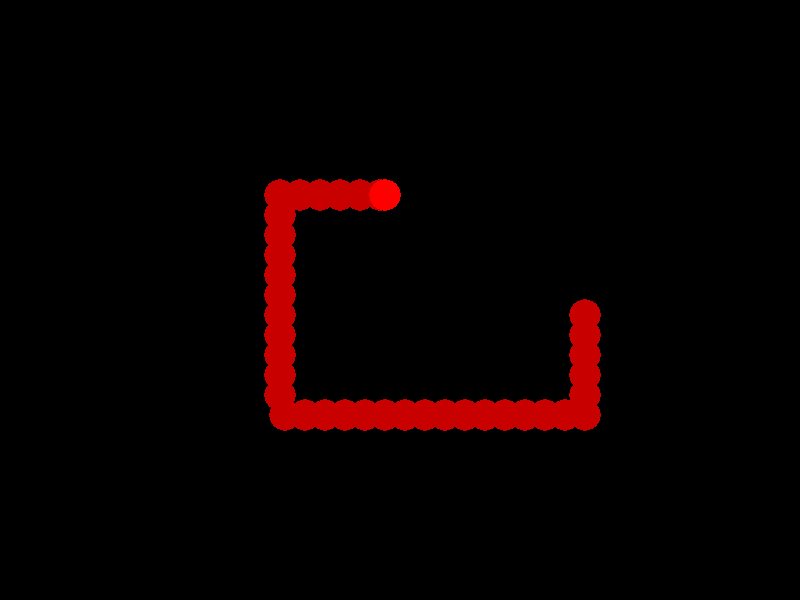
\includegraphics{ss-1-death.png}
Right now the snake actually doesn't die it just logs to the console. For the death animation, lets
turn the body red and then gradually remove body parts until we get to the head.

Now for this kind of animation you want it to take a while to show. If you implement this in the
\emph{upateActor} method then it might happen pretty quickly since that is called 60 times a second.
We can use a timed callback to do this where we can control how often it is called.

Callbacks fall under a category called \emph{behaviours}. These are generally useful kinds of activities
that can apply to any actors. To utilize \emph{behaviours} you create a \emph{BehaviourManager}, which is just
a special actor, and then use it to assign behaviours.

\begin{Verbatim}[commandchars=\\\{\},numbers=left,firstnumber=1,stepnumber=1]
\PYG{k+kn}{import} \PYG{n+nn}{pygame}

\PYG{k+kn}{import} \PYG{n+nn}{serge.engine}
\PYG{k+kn}{import} \PYG{n+nn}{serge.actor}
\PYG{k+kn}{import} \PYG{n+nn}{serge.blocks.visualblocks}
\PYG{k+kn}{import} \PYG{n+nn}{serge.blocks.utils}
\PYG{k+kn}{import} \PYG{n+nn}{serge.blocks.directions}
\PYG{k+kn}{import} \PYG{n+nn}{serge.blocks.behaviours}

\PYG{k}{class} \PYG{n+nc}{Snake}\PYG{p}{(}\PYG{n}{serge}\PYG{o}{.}\PYG{n}{actor}\PYG{o}{.}\PYG{n}{CompositeActor}\PYG{p}{)}\PYG{p}{:}
    \PYG{l+s+sd}{"""Represents the snake"""}

    \PYG{k}{def} \PYG{n+nf}{\PYGZus{}\PYGZus{}init\PYGZus{}\PYGZus{}}\PYG{p}{(}\PYG{n+nb+bp}{self}\PYG{p}{)}\PYG{p}{:}
        \PYG{l+s+sd}{"""Initialise the snake"""}
        \PYG{n+nb}{super}\PYG{p}{(}\PYG{n}{Snake}\PYG{p}{,} \PYG{n+nb+bp}{self}\PYG{p}{)}\PYG{o}{.}\PYG{n}{\PYGZus{}\PYGZus{}init\PYGZus{}\PYGZus{}}\PYG{p}{(}\PYG{l+s}{'}\PYG{l+s}{snake}\PYG{l+s}{'}\PYG{p}{,} \PYG{l+s}{'}\PYG{l+s}{snake-head}\PYG{l+s}{'}\PYG{p}{)}
        \PYG{n+nb+bp}{self}\PYG{o}{.}\PYG{n}{visual} \PYG{o}{=} \PYG{n}{serge}\PYG{o}{.}\PYG{n}{blocks}\PYG{o}{.}\PYG{n}{visualblocks}\PYG{o}{.}\PYG{n}{Circle}\PYG{p}{(}\PYG{l+m+mi}{16}\PYG{p}{,} \PYG{p}{(}\PYG{l+m+mi}{0}\PYG{p}{,}\PYG{l+m+mi}{255}\PYG{p}{,}\PYG{l+m+mi}{0}\PYG{p}{)}\PYG{p}{)}
        \PYG{n+nb+bp}{self}\PYG{o}{.}\PYG{n}{setLayerName}\PYG{p}{(}\PYG{l+s}{'}\PYG{l+s}{middle}\PYG{l+s}{'}\PYG{p}{)}
        \PYG{n+nb+bp}{self}\PYG{o}{.}\PYG{n}{current\PYGZus{}direction} \PYG{o}{=} \PYG{n}{serge}\PYG{o}{.}\PYG{n}{blocks}\PYG{o}{.}\PYG{n}{directions}\PYG{o}{.}\PYG{n}{N}
        \PYG{n+nb+bp}{self}\PYG{o}{.}\PYG{n}{is\PYGZus{}dying} \PYG{o}{=} \PYG{n+nb+bp}{False}

    \PYG{k}{def} \PYG{n+nf}{addedToWorld}\PYG{p}{(}\PYG{n+nb+bp}{self}\PYG{p}{,} \PYG{n}{world}\PYG{p}{)}\PYG{p}{:}
        \PYG{l+s+sd}{"""The snake was added to the world"""}
        \PYG{n+nb}{super}\PYG{p}{(}\PYG{n}{Snake}\PYG{p}{,} \PYG{n+nb+bp}{self}\PYG{p}{)}\PYG{o}{.}\PYG{n}{addedToWorld}\PYG{p}{(}\PYG{n}{world}\PYG{p}{)}
        \PYG{c}{\PYGZsh{}}
        \PYG{n+nb+bp}{self}\PYG{o}{.}\PYG{n}{keyboard} \PYG{o}{=} \PYG{n}{serge}\PYG{o}{.}\PYG{n}{engine}\PYG{o}{.}\PYG{n}{CurrentEngine}\PYG{p}{(}\PYG{p}{)}\PYG{o}{.}\PYG{n}{getKeyboard}\PYG{p}{(}\PYG{p}{)}
        \PYG{n+nb+bp}{self}\PYG{o}{.}\PYG{n}{manager} \PYG{o}{=} \PYG{n}{serge}\PYG{o}{.}\PYG{n}{blocks}\PYG{o}{.}\PYG{n}{behaviours}\PYG{o}{.}\PYG{n}{BehaviourManager}\PYG{p}{(}\PYG{l+s}{'}\PYG{l+s}{manager}\PYG{l+s}{'}\PYG{p}{,} \PYG{l+s}{'}\PYG{l+s}{behaviour-manager}\PYG{l+s}{'}\PYG{p}{)}
        \PYG{n}{world}\PYG{o}{.}\PYG{n}{addActor}\PYG{p}{(}\PYG{n+nb+bp}{self}\PYG{o}{.}\PYG{n}{manager}\PYG{p}{)}

    \PYG{k}{def} \PYG{n+nf}{updateActor}\PYG{p}{(}\PYG{n+nb+bp}{self}\PYG{p}{,} \PYG{n}{interval}\PYG{p}{,} \PYG{n}{world}\PYG{p}{)}\PYG{p}{:}
        \PYG{l+s+sd}{"""Update the snake"""}
        \PYG{n+nb}{super}\PYG{p}{(}\PYG{n}{Snake}\PYG{p}{,} \PYG{n+nb+bp}{self}\PYG{p}{)}\PYG{o}{.}\PYG{n}{updateActor}\PYG{p}{(}\PYG{n}{interval}\PYG{p}{,} \PYG{n}{world}\PYG{p}{)}
        \PYG{c}{\PYGZsh{}}
        \PYG{c}{\PYGZsh{} Move the head}
        \PYG{k}{if} \PYG{n+nb+bp}{self}\PYG{o}{.}\PYG{n}{keyboard}\PYG{o}{.}\PYG{n}{isClicked}\PYG{p}{(}\PYG{n}{pygame}\PYG{o}{.}\PYG{n}{K\PYGZus{}LEFT}\PYG{p}{)}\PYG{p}{:}
            \PYG{n}{rotation} \PYG{o}{=} \PYG{o}{+}\PYG{l+m+mi}{90}
        \PYG{k}{elif} \PYG{n+nb+bp}{self}\PYG{o}{.}\PYG{n}{keyboard}\PYG{o}{.}\PYG{n}{isClicked}\PYG{p}{(}\PYG{n}{pygame}\PYG{o}{.}\PYG{n}{K\PYGZus{}RIGHT}\PYG{p}{)}\PYG{p}{:}
            \PYG{n}{rotation} \PYG{o}{=} \PYG{o}{-}\PYG{l+m+mi}{90}
        \PYG{k}{else}\PYG{p}{:}
            \PYG{n}{rotation} \PYG{o}{=} \PYG{l+m+mi}{0}
        \PYG{c}{\PYGZsh{}}
        \PYG{c}{\PYGZsh{} Change direction}
        \PYG{k}{if} \PYG{n}{rotation}\PYG{p}{:}
            \PYG{n}{current\PYGZus{}angle} \PYG{o}{=} \PYG{n}{serge}\PYG{o}{.}\PYG{n}{blocks}\PYG{o}{.}\PYG{n}{directions}\PYG{o}{.}\PYG{n}{getAngleFromCardinal}\PYG{p}{(}\PYG{n+nb+bp}{self}\PYG{o}{.}\PYG{n}{current\PYGZus{}direction}\PYG{p}{)}
            \PYG{n+nb+bp}{self}\PYG{o}{.}\PYG{n}{current\PYGZus{}direction} \PYG{o}{=} \PYG{n}{serge}\PYG{o}{.}\PYG{n}{blocks}\PYG{o}{.}\PYG{n}{directions}\PYG{o}{.}\PYG{n}{getCardinalFromAngle}\PYG{p}{(}\PYG{n}{current\PYGZus{}angle}\PYG{o}{+}\PYG{n}{rotation}\PYG{p}{)}
        \PYG{c}{\PYGZsh{}}
        \PYG{c}{\PYGZsh{} Move}
        \PYG{k}{if} \PYG{o+ow}{not} \PYG{n+nb+bp}{self}\PYG{o}{.}\PYG{n}{is\PYGZus{}dying}\PYG{p}{:}
            \PYG{n}{offset} \PYG{o}{=} \PYG{l+m+mi}{5}\PYG{o}{*}\PYG{n}{serge}\PYG{o}{.}\PYG{n}{blocks}\PYG{o}{.}\PYG{n}{directions}\PYG{o}{.}\PYG{n}{getVectorFromCardinal}\PYG{p}{(}\PYG{n+nb+bp}{self}\PYG{o}{.}\PYG{n}{current\PYGZus{}direction}\PYG{p}{)}
            \PYG{n+nb+bp}{self}\PYG{o}{.}\PYG{n}{move}\PYG{p}{(}\PYG{o}{*}\PYG{n}{offset}\PYG{p}{)}
            \PYG{c}{\PYGZsh{}}
            \PYG{c}{\PYGZsh{} Add a new segment if needed}
            \PYG{k}{if} \PYG{o+ow}{not} \PYG{n+nb+bp}{self}\PYG{o}{.}\PYG{n}{getChildren}\PYG{p}{(}\PYG{p}{)} \PYG{o+ow}{or} \PYG{n+nb+bp}{self}\PYG{o}{.}\PYG{n}{getDistanceFrom}\PYG{p}{(}\PYG{n+nb+bp}{self}\PYG{o}{.}\PYG{n}{getChildren}\PYG{p}{(}\PYG{p}{)}\PYG{p}{[}\PYG{o}{-}\PYG{l+m+mi}{1}\PYG{p}{]}\PYG{p}{)} \PYG{o}{\textgreater{}} \PYG{l+m+mi}{16}\PYG{p}{:}
                \PYG{n+nb+bp}{self}\PYG{o}{.}\PYG{n}{addSegment}\PYG{p}{(}\PYG{p}{)}
            \PYG{c}{\PYGZsh{}}
            \PYG{c}{\PYGZsh{} Check if we hit the body}
            \PYG{k}{if} \PYG{n+nb+bp}{self}\PYG{o}{.}\PYG{n}{hitBody}\PYG{p}{(}\PYG{p}{)}\PYG{p}{:}
                \PYG{n+nb+bp}{self}\PYG{o}{.}\PYG{n}{initiateDeathAnimation}\PYG{p}{(}\PYG{p}{)}

    \PYG{k}{def} \PYG{n+nf}{addSegment}\PYG{p}{(}\PYG{n+nb+bp}{self}\PYG{p}{)}\PYG{p}{:}
        \PYG{l+s+sd}{"""Add a new body segment"""}
        \PYG{n}{segment} \PYG{o}{=} \PYG{n}{serge}\PYG{o}{.}\PYG{n}{actor}\PYG{o}{.}\PYG{n}{Actor}\PYG{p}{(}\PYG{l+s}{'}\PYG{l+s}{segment}\PYG{l+s}{'}\PYG{p}{)}
        \PYG{n}{segment}\PYG{o}{.}\PYG{n}{visual} \PYG{o}{=} \PYG{n}{serge}\PYG{o}{.}\PYG{n}{blocks}\PYG{o}{.}\PYG{n}{visualblocks}\PYG{o}{.}\PYG{n}{Circle}\PYG{p}{(}\PYG{l+m+mi}{16}\PYG{p}{,} \PYG{p}{(}\PYG{l+m+mi}{0}\PYG{p}{,}\PYG{l+m+mi}{200}\PYG{p}{,}\PYG{l+m+mi}{0}\PYG{p}{)}\PYG{p}{)}
        \PYG{n}{segment}\PYG{o}{.}\PYG{n}{setLayerName}\PYG{p}{(}\PYG{l+s}{'}\PYG{l+s}{middle}\PYG{l+s}{'}\PYG{p}{)}
        \PYG{n}{segment}\PYG{o}{.}\PYG{n}{moveTo}\PYG{p}{(}\PYG{n+nb+bp}{self}\PYG{o}{.}\PYG{n}{x}\PYG{p}{,} \PYG{n+nb+bp}{self}\PYG{o}{.}\PYG{n}{y}\PYG{p}{)}
        \PYG{n+nb+bp}{self}\PYG{o}{.}\PYG{n}{addChild}\PYG{p}{(}\PYG{n}{segment}\PYG{p}{)}

    \PYG{k}{def} \PYG{n+nf}{hitBody}\PYG{p}{(}\PYG{n+nb+bp}{self}\PYG{p}{)}\PYG{p}{:}
        \PYG{l+s+sd}{"""Return True if the head has hit the body}

\PYG{l+s+sd}{        Look to see if we overlap with any body segment except the last}
\PYG{l+s+sd}{        (we are allowed to overlap the last since we just put it down)}

\PYG{l+s+sd}{        """}
        \PYG{k}{for} \PYG{n}{segment} \PYG{o+ow}{in} \PYG{n+nb+bp}{self}\PYG{o}{.}\PYG{n}{getChildren}\PYG{p}{(}\PYG{p}{)}\PYG{p}{[}\PYG{p}{:}\PYG{o}{-}\PYG{l+m+mi}{1}\PYG{p}{]}\PYG{p}{:}
            \PYG{k}{if} \PYG{n+nb+bp}{self}\PYG{o}{.}\PYG{n}{getDistanceFrom}\PYG{p}{(}\PYG{n}{segment}\PYG{p}{)} \PYG{o}{\textless{}} \PYG{l+m+mi}{16}\PYG{p}{:}
                \PYG{k}{return} \PYG{n+nb+bp}{True}
        \PYG{k}{return} \PYG{n+nb+bp}{False}

    \PYG{k}{def} \PYG{n+nf}{initiateDeathAnimation}\PYG{p}{(}\PYG{n+nb+bp}{self}\PYG{p}{)}\PYG{p}{:}
        \PYG{l+s+sd}{"""Begin showing the death of the snake"""}
        \PYG{n+nb+bp}{self}\PYG{o}{.}\PYG{n}{log}\PYG{o}{.}\PYG{n}{info}\PYG{p}{(}\PYG{l+s}{'}\PYG{l+s}{Snake died!}\PYG{l+s}{'}\PYG{p}{)}
        \PYG{n+nb+bp}{self}\PYG{o}{.}\PYG{n}{animation} \PYG{o}{=} \PYG{n+nb+bp}{self}\PYG{o}{.}\PYG{n}{manager}\PYG{o}{.}\PYG{n}{assignBehaviour}\PYG{p}{(}\PYG{n+nb+bp}{self}\PYG{p}{,}
            \PYG{n}{serge}\PYG{o}{.}\PYG{n}{blocks}\PYG{o}{.}\PYG{n}{behaviours}\PYG{o}{.}\PYG{n}{TimedCallback}\PYG{p}{(}\PYG{l+m+mi}{1000}\PYG{o}{/}\PYG{n+nb}{len}\PYG{p}{(}\PYG{n+nb+bp}{self}\PYG{o}{.}\PYG{n}{getChildren}\PYG{p}{(}\PYG{p}{)}\PYG{p}{)}\PYG{p}{,} \PYG{n+nb+bp}{self}\PYG{o}{.}\PYG{n}{removeTail}\PYG{p}{)}\PYG{p}{,} \PYG{l+s}{'}\PYG{l+s}{death-animation}\PYG{l+s}{'}\PYG{p}{)}
        \PYG{n+nb+bp}{self}\PYG{o}{.}\PYG{n}{is\PYGZus{}dying} \PYG{o}{=} \PYG{n+nb+bp}{True}
        \PYG{k}{for} \PYG{n}{segment} \PYG{o+ow}{in} \PYG{n+nb+bp}{self}\PYG{o}{.}\PYG{n}{getChildren}\PYG{p}{(}\PYG{p}{)}\PYG{p}{:}
            \PYG{n}{segment}\PYG{o}{.}\PYG{n}{visual}\PYG{o}{.}\PYG{n}{colour} \PYG{o}{=} \PYG{p}{(}\PYG{l+m+mi}{200}\PYG{p}{,} \PYG{l+m+mi}{0}\PYG{p}{,} \PYG{l+m+mi}{0}\PYG{p}{)}
        \PYG{n+nb+bp}{self}\PYG{o}{.}\PYG{n}{visual}\PYG{o}{.}\PYG{n}{colour} \PYG{o}{=} \PYG{p}{(}\PYG{l+m+mi}{255}\PYG{p}{,} \PYG{l+m+mi}{0}\PYG{p}{,} \PYG{l+m+mi}{0}\PYG{p}{)}

    \PYG{k}{def} \PYG{n+nf}{removeTail}\PYG{p}{(}\PYG{n+nb+bp}{self}\PYG{p}{,} \PYG{n}{world}\PYG{p}{,} \PYG{n}{actor}\PYG{p}{,} \PYG{n}{interval}\PYG{p}{)}\PYG{p}{:}
        \PYG{l+s+sd}{"""Remove part of the tail"""}
        \PYG{n+nb+bp}{self}\PYG{o}{.}\PYG{n}{log}\PYG{o}{.}\PYG{n}{debug}\PYG{p}{(}\PYG{l+s}{'}\PYG{l+s}{Removing part of the tail}\PYG{l+s}{'}\PYG{p}{)}
        \PYG{k}{if} \PYG{n+nb+bp}{self}\PYG{o}{.}\PYG{n}{getChildren}\PYG{p}{(}\PYG{p}{)}\PYG{p}{:}
            \PYG{n+nb+bp}{self}\PYG{o}{.}\PYG{n}{removeChild}\PYG{p}{(}\PYG{n+nb+bp}{self}\PYG{o}{.}\PYG{n}{getChildren}\PYG{p}{(}\PYG{p}{)}\PYG{p}{[}\PYG{l+m+mi}{0}\PYG{p}{]}\PYG{p}{)}
        \PYG{k}{else}\PYG{p}{:}
            \PYG{n+nb+bp}{self}\PYG{o}{.}\PYG{n}{animation}\PYG{o}{.}\PYG{n}{markComplete}\PYG{p}{(}\PYG{p}{)}

\PYG{c}{\PYGZsh{} Create the engine}
\PYG{n}{engine} \PYG{o}{=} \PYG{n}{serge}\PYG{o}{.}\PYG{n}{blocks}\PYG{o}{.}\PYG{n}{utils}\PYG{o}{.}\PYG{n}{getSimpleSetup}\PYG{p}{(}\PYG{l+m+mi}{800}\PYG{p}{,} \PYG{l+m+mi}{600}\PYG{p}{)}
\PYG{n}{world} \PYG{o}{=} \PYG{n}{engine}\PYG{o}{.}\PYG{n}{getWorld}\PYG{p}{(}\PYG{l+s}{'}\PYG{l+s}{lab}\PYG{l+s}{'}\PYG{p}{)}

\PYG{c}{\PYGZsh{} Create the snake}
\PYG{n}{snake} \PYG{o}{=} \PYG{n}{Snake}\PYG{p}{(}\PYG{p}{)}
\PYG{n}{world}\PYG{o}{.}\PYG{n}{addActor}\PYG{p}{(}\PYG{n}{snake}\PYG{p}{)}
\PYG{n}{snake}\PYG{o}{.}\PYG{n}{moveTo}\PYG{p}{(}\PYG{l+m+mi}{400}\PYG{p}{,} \PYG{l+m+mi}{300}\PYG{p}{)}

\PYG{c}{\PYGZsh{} Run the game}
\PYG{n}{engine}\PYG{o}{.}\PYG{n}{run}\PYG{p}{(}\PYG{l+m+mi}{60}\PYG{p}{)}
\end{Verbatim}

There is a bit of housekeeping we have to do here. On line 19 we create a new property \emph{is\_dying} which we will set
when the snake is dying. When this is true we do not want to move the snake, add bodies or check for death (again) so
we protect some of the lines in the \emph{updateActor} method to prevent them being called.

The reset of the updates create the \emph{manager} and then use it to assign the \emph{callback}. We call the \emph{removeTail}
method to gradually remove our children. The time interval is set to make sure if takes about a second
to remove the whole tail. When it is done it calls the \emph{markComplete}
method on the \emph{behaviour} to tell the engine that it can be discarded as we wont need it again.


\subsection{Restarting The Game}
\label{tutorial-1:restarting-the-game}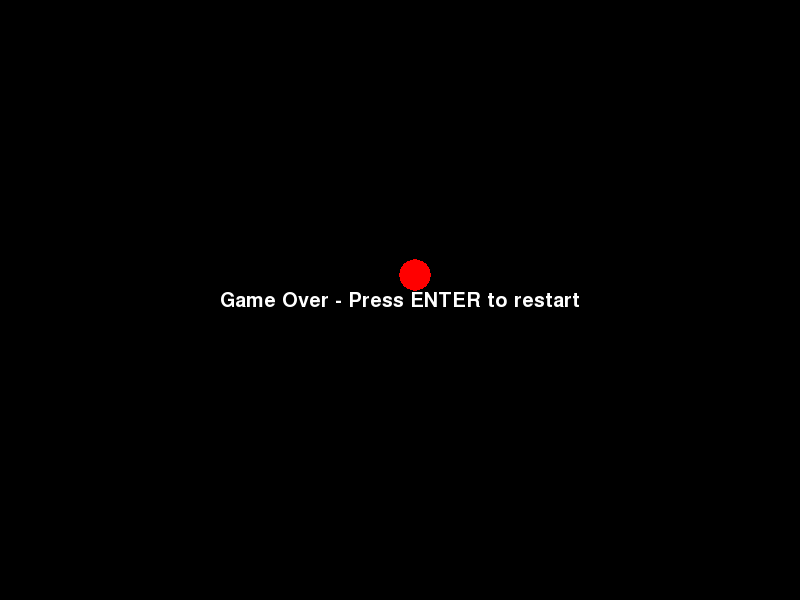
\includegraphics{ss-1-restart.png}
There isn't anything to do after you die now so let's add some text and a way to restart.

\begin{Verbatim}[commandchars=\\\{\},numbers=left,firstnumber=1,stepnumber=1]
\PYG{k+kn}{import} \PYG{n+nn}{pygame}

\PYG{k+kn}{import} \PYG{n+nn}{serge.engine}
\PYG{k+kn}{import} \PYG{n+nn}{serge.actor}
\PYG{k+kn}{import} \PYG{n+nn}{serge.blocks.visualblocks}
\PYG{k+kn}{import} \PYG{n+nn}{serge.blocks.utils}
\PYG{k+kn}{import} \PYG{n+nn}{serge.blocks.directions}
\PYG{k+kn}{import} \PYG{n+nn}{serge.blocks.behaviours}

\PYG{k}{class} \PYG{n+nc}{Snake}\PYG{p}{(}\PYG{n}{serge}\PYG{o}{.}\PYG{n}{actor}\PYG{o}{.}\PYG{n}{CompositeActor}\PYG{p}{)}\PYG{p}{:}
    \PYG{l+s+sd}{"""Represents the snake"""}

    \PYG{k}{def} \PYG{n+nf}{\PYGZus{}\PYGZus{}init\PYGZus{}\PYGZus{}}\PYG{p}{(}\PYG{n+nb+bp}{self}\PYG{p}{)}\PYG{p}{:}
        \PYG{l+s+sd}{"""Initialise the snake"""}
        \PYG{n+nb}{super}\PYG{p}{(}\PYG{n}{Snake}\PYG{p}{,} \PYG{n+nb+bp}{self}\PYG{p}{)}\PYG{o}{.}\PYG{n}{\PYGZus{}\PYGZus{}init\PYGZus{}\PYGZus{}}\PYG{p}{(}\PYG{l+s}{'}\PYG{l+s}{snake}\PYG{l+s}{'}\PYG{p}{,} \PYG{l+s}{'}\PYG{l+s}{snake-head}\PYG{l+s}{'}\PYG{p}{)}
        \PYG{n+nb+bp}{self}\PYG{o}{.}\PYG{n}{visual} \PYG{o}{=} \PYG{n}{serge}\PYG{o}{.}\PYG{n}{blocks}\PYG{o}{.}\PYG{n}{visualblocks}\PYG{o}{.}\PYG{n}{Circle}\PYG{p}{(}\PYG{l+m+mi}{16}\PYG{p}{,} \PYG{p}{(}\PYG{l+m+mi}{0}\PYG{p}{,}\PYG{l+m+mi}{255}\PYG{p}{,}\PYG{l+m+mi}{0}\PYG{p}{)}\PYG{p}{)}
        \PYG{n+nb+bp}{self}\PYG{o}{.}\PYG{n}{setLayerName}\PYG{p}{(}\PYG{l+s}{'}\PYG{l+s}{middle}\PYG{l+s}{'}\PYG{p}{)}
        \PYG{n+nb+bp}{self}\PYG{o}{.}\PYG{n}{current\PYGZus{}direction} \PYG{o}{=} \PYG{n}{serge}\PYG{o}{.}\PYG{n}{blocks}\PYG{o}{.}\PYG{n}{directions}\PYG{o}{.}\PYG{n}{N}
        \PYG{n+nb+bp}{self}\PYG{o}{.}\PYG{n}{is\PYGZus{}dying} \PYG{o}{=} \PYG{n+nb+bp}{False}

    \PYG{k}{def} \PYG{n+nf}{addedToWorld}\PYG{p}{(}\PYG{n+nb+bp}{self}\PYG{p}{,} \PYG{n}{world}\PYG{p}{)}\PYG{p}{:}
        \PYG{l+s+sd}{"""The snake was added to the world"""}
        \PYG{n+nb}{super}\PYG{p}{(}\PYG{n}{Snake}\PYG{p}{,} \PYG{n+nb+bp}{self}\PYG{p}{)}\PYG{o}{.}\PYG{n}{addedToWorld}\PYG{p}{(}\PYG{n}{world}\PYG{p}{)}
        \PYG{c}{\PYGZsh{}}
        \PYG{n+nb+bp}{self}\PYG{o}{.}\PYG{n}{keyboard} \PYG{o}{=} \PYG{n}{serge}\PYG{o}{.}\PYG{n}{engine}\PYG{o}{.}\PYG{n}{CurrentEngine}\PYG{p}{(}\PYG{p}{)}\PYG{o}{.}\PYG{n}{getKeyboard}\PYG{p}{(}\PYG{p}{)}
        \PYG{n+nb+bp}{self}\PYG{o}{.}\PYG{n}{manager} \PYG{o}{=} \PYG{n}{serge}\PYG{o}{.}\PYG{n}{blocks}\PYG{o}{.}\PYG{n}{behaviours}\PYG{o}{.}\PYG{n}{BehaviourManager}\PYG{p}{(}\PYG{l+s}{'}\PYG{l+s}{manager}\PYG{l+s}{'}\PYG{p}{,} \PYG{l+s}{'}\PYG{l+s}{behaviour-manager}\PYG{l+s}{'}\PYG{p}{)}
        \PYG{n}{world}\PYG{o}{.}\PYG{n}{addActor}\PYG{p}{(}\PYG{n+nb+bp}{self}\PYG{o}{.}\PYG{n}{manager}\PYG{p}{)}
        \PYG{c}{\PYGZsh{}}
        \PYG{n+nb+bp}{self}\PYG{o}{.}\PYG{n}{restart\PYGZus{}text} \PYG{o}{=} \PYG{n}{serge}\PYG{o}{.}\PYG{n}{blocks}\PYG{o}{.}\PYG{n}{utils}\PYG{o}{.}\PYG{n}{addVisualActorToWorld}\PYG{p}{(}\PYG{n}{world}\PYG{p}{,} \PYG{l+s}{'}\PYG{l+s}{text}\PYG{l+s}{'}\PYG{p}{,} \PYG{l+s}{'}\PYG{l+s}{restart}\PYG{l+s}{'}\PYG{p}{,}
            \PYG{n}{serge}\PYG{o}{.}\PYG{n}{visual}\PYG{o}{.}\PYG{n}{Text}\PYG{p}{(}\PYG{l+s}{'}\PYG{l+s}{Game Over - Press ENTER to restart}\PYG{l+s}{'}\PYG{p}{,} \PYG{p}{(}\PYG{l+m+mi}{255}\PYG{p}{,} \PYG{l+m+mi}{255}\PYG{p}{,} \PYG{l+m+mi}{255}\PYG{p}{)}\PYG{p}{,} \PYG{n}{font\PYGZus{}size}\PYG{o}{=}\PYG{l+m+mi}{20}\PYG{p}{)}\PYG{p}{,}
            \PYG{n}{layer\PYGZus{}name}\PYG{o}{=}\PYG{l+s}{'}\PYG{l+s}{front}\PYG{l+s}{'}\PYG{p}{,}
            \PYG{n}{center\PYGZus{}position}\PYG{o}{=}\PYG{p}{(}\PYG{l+m+mi}{400}\PYG{p}{,} \PYG{l+m+mi}{300}\PYG{p}{)}\PYG{p}{)}
        \PYG{n+nb+bp}{self}\PYG{o}{.}\PYG{n}{restart\PYGZus{}text}\PYG{o}{.}\PYG{n}{visible} \PYG{o}{=} \PYG{n+nb+bp}{False}

    \PYG{k}{def} \PYG{n+nf}{updateActor}\PYG{p}{(}\PYG{n+nb+bp}{self}\PYG{p}{,} \PYG{n}{interval}\PYG{p}{,} \PYG{n}{world}\PYG{p}{)}\PYG{p}{:}
        \PYG{l+s+sd}{"""Update the snake"""}
        \PYG{n+nb}{super}\PYG{p}{(}\PYG{n}{Snake}\PYG{p}{,} \PYG{n+nb+bp}{self}\PYG{p}{)}\PYG{o}{.}\PYG{n}{updateActor}\PYG{p}{(}\PYG{n}{interval}\PYG{p}{,} \PYG{n}{world}\PYG{p}{)}
        \PYG{c}{\PYGZsh{}}
        \PYG{c}{\PYGZsh{} Move the head}
        \PYG{k}{if} \PYG{n+nb+bp}{self}\PYG{o}{.}\PYG{n}{keyboard}\PYG{o}{.}\PYG{n}{isClicked}\PYG{p}{(}\PYG{n}{pygame}\PYG{o}{.}\PYG{n}{K\PYGZus{}LEFT}\PYG{p}{)}\PYG{p}{:}
            \PYG{n}{rotation} \PYG{o}{=} \PYG{o}{+}\PYG{l+m+mi}{90}
        \PYG{k}{elif} \PYG{n+nb+bp}{self}\PYG{o}{.}\PYG{n}{keyboard}\PYG{o}{.}\PYG{n}{isClicked}\PYG{p}{(}\PYG{n}{pygame}\PYG{o}{.}\PYG{n}{K\PYGZus{}RIGHT}\PYG{p}{)}\PYG{p}{:}
            \PYG{n}{rotation} \PYG{o}{=} \PYG{o}{-}\PYG{l+m+mi}{90}
        \PYG{k}{else}\PYG{p}{:}
            \PYG{n}{rotation} \PYG{o}{=} \PYG{l+m+mi}{0}
        \PYG{c}{\PYGZsh{}}
        \PYG{c}{\PYGZsh{} Change direction}
        \PYG{k}{if} \PYG{n}{rotation}\PYG{p}{:}
            \PYG{n}{current\PYGZus{}angle} \PYG{o}{=} \PYG{n}{serge}\PYG{o}{.}\PYG{n}{blocks}\PYG{o}{.}\PYG{n}{directions}\PYG{o}{.}\PYG{n}{getAngleFromCardinal}\PYG{p}{(}\PYG{n+nb+bp}{self}\PYG{o}{.}\PYG{n}{current\PYGZus{}direction}\PYG{p}{)}
            \PYG{n+nb+bp}{self}\PYG{o}{.}\PYG{n}{current\PYGZus{}direction} \PYG{o}{=} \PYG{n}{serge}\PYG{o}{.}\PYG{n}{blocks}\PYG{o}{.}\PYG{n}{directions}\PYG{o}{.}\PYG{n}{getCardinalFromAngle}\PYG{p}{(}\PYG{n}{current\PYGZus{}angle}\PYG{o}{+}\PYG{n}{rotation}\PYG{p}{)}
        \PYG{c}{\PYGZsh{}}
        \PYG{c}{\PYGZsh{} Move}
        \PYG{k}{if} \PYG{o+ow}{not} \PYG{n+nb+bp}{self}\PYG{o}{.}\PYG{n}{is\PYGZus{}dying}\PYG{p}{:}
            \PYG{n}{offset} \PYG{o}{=} \PYG{l+m+mi}{5}\PYG{o}{*}\PYG{n}{serge}\PYG{o}{.}\PYG{n}{blocks}\PYG{o}{.}\PYG{n}{directions}\PYG{o}{.}\PYG{n}{getVectorFromCardinal}\PYG{p}{(}\PYG{n+nb+bp}{self}\PYG{o}{.}\PYG{n}{current\PYGZus{}direction}\PYG{p}{)}
            \PYG{n+nb+bp}{self}\PYG{o}{.}\PYG{n}{move}\PYG{p}{(}\PYG{o}{*}\PYG{n}{offset}\PYG{p}{)}
            \PYG{c}{\PYGZsh{}}
            \PYG{c}{\PYGZsh{} Add a new segment if needed}
            \PYG{k}{if} \PYG{o+ow}{not} \PYG{n+nb+bp}{self}\PYG{o}{.}\PYG{n}{getChildren}\PYG{p}{(}\PYG{p}{)} \PYG{o+ow}{or} \PYG{n+nb+bp}{self}\PYG{o}{.}\PYG{n}{getDistanceFrom}\PYG{p}{(}\PYG{n+nb+bp}{self}\PYG{o}{.}\PYG{n}{getChildren}\PYG{p}{(}\PYG{p}{)}\PYG{p}{[}\PYG{o}{-}\PYG{l+m+mi}{1}\PYG{p}{]}\PYG{p}{)} \PYG{o}{\textgreater{}} \PYG{l+m+mi}{16}\PYG{p}{:}
                \PYG{n+nb+bp}{self}\PYG{o}{.}\PYG{n}{addSegment}\PYG{p}{(}\PYG{p}{)}
            \PYG{c}{\PYGZsh{}}
            \PYG{c}{\PYGZsh{} Check if we hit the body}
            \PYG{k}{if} \PYG{n+nb+bp}{self}\PYG{o}{.}\PYG{n}{hitBody}\PYG{p}{(}\PYG{p}{)}\PYG{p}{:}
                \PYG{n+nb+bp}{self}\PYG{o}{.}\PYG{n}{initiateDeathAnimation}\PYG{p}{(}\PYG{p}{)}
        \PYG{k}{elif} \PYG{n+nb+bp}{self}\PYG{o}{.}\PYG{n}{animation}\PYG{o}{.}\PYG{n}{isComplete}\PYG{p}{(}\PYG{p}{)}\PYG{p}{:}
            \PYG{k}{if} \PYG{n+nb+bp}{self}\PYG{o}{.}\PYG{n}{keyboard}\PYG{o}{.}\PYG{n}{isClicked}\PYG{p}{(}\PYG{n}{pygame}\PYG{o}{.}\PYG{n}{K\PYGZus{}KP\PYGZus{}ENTER}\PYG{p}{)} \PYG{o+ow}{or} \PYG{n+nb+bp}{self}\PYG{o}{.}\PYG{n}{keyboard}\PYG{o}{.}\PYG{n}{isClicked}\PYG{p}{(}\PYG{n}{pygame}\PYG{o}{.}\PYG{n}{K\PYGZus{}RETURN}\PYG{p}{)}\PYG{p}{:}
                \PYG{n+nb+bp}{self}\PYG{o}{.}\PYG{n}{restartGame}\PYG{p}{(}\PYG{p}{)}

    \PYG{k}{def} \PYG{n+nf}{addSegment}\PYG{p}{(}\PYG{n+nb+bp}{self}\PYG{p}{)}\PYG{p}{:}
        \PYG{l+s+sd}{"""Add a new body segment"""}
        \PYG{n}{segment} \PYG{o}{=} \PYG{n}{serge}\PYG{o}{.}\PYG{n}{actor}\PYG{o}{.}\PYG{n}{Actor}\PYG{p}{(}\PYG{l+s}{'}\PYG{l+s}{segment}\PYG{l+s}{'}\PYG{p}{)}
        \PYG{n}{segment}\PYG{o}{.}\PYG{n}{visual} \PYG{o}{=} \PYG{n}{serge}\PYG{o}{.}\PYG{n}{blocks}\PYG{o}{.}\PYG{n}{visualblocks}\PYG{o}{.}\PYG{n}{Circle}\PYG{p}{(}\PYG{l+m+mi}{16}\PYG{p}{,} \PYG{p}{(}\PYG{l+m+mi}{0}\PYG{p}{,}\PYG{l+m+mi}{200}\PYG{p}{,}\PYG{l+m+mi}{0}\PYG{p}{)}\PYG{p}{)}
        \PYG{n}{segment}\PYG{o}{.}\PYG{n}{setLayerName}\PYG{p}{(}\PYG{l+s}{'}\PYG{l+s}{middle}\PYG{l+s}{'}\PYG{p}{)}
        \PYG{n}{segment}\PYG{o}{.}\PYG{n}{moveTo}\PYG{p}{(}\PYG{n+nb+bp}{self}\PYG{o}{.}\PYG{n}{x}\PYG{p}{,} \PYG{n+nb+bp}{self}\PYG{o}{.}\PYG{n}{y}\PYG{p}{)}
        \PYG{n+nb+bp}{self}\PYG{o}{.}\PYG{n}{addChild}\PYG{p}{(}\PYG{n}{segment}\PYG{p}{)}

    \PYG{k}{def} \PYG{n+nf}{hitBody}\PYG{p}{(}\PYG{n+nb+bp}{self}\PYG{p}{)}\PYG{p}{:}
        \PYG{l+s+sd}{"""Return True if the head has hit the body}

\PYG{l+s+sd}{        Look to see if we overlap with any body segment except the last}
\PYG{l+s+sd}{        (we are allowed to overlap the last since we just put it down)}

\PYG{l+s+sd}{        """}
        \PYG{k}{for} \PYG{n}{segment} \PYG{o+ow}{in} \PYG{n+nb+bp}{self}\PYG{o}{.}\PYG{n}{getChildren}\PYG{p}{(}\PYG{p}{)}\PYG{p}{[}\PYG{p}{:}\PYG{o}{-}\PYG{l+m+mi}{1}\PYG{p}{]}\PYG{p}{:}
            \PYG{k}{if} \PYG{n+nb+bp}{self}\PYG{o}{.}\PYG{n}{getDistanceFrom}\PYG{p}{(}\PYG{n}{segment}\PYG{p}{)} \PYG{o}{\textless{}} \PYG{l+m+mi}{16}\PYG{p}{:}
                \PYG{k}{return} \PYG{n+nb+bp}{True}
        \PYG{k}{return} \PYG{n+nb+bp}{False}

    \PYG{k}{def} \PYG{n+nf}{initiateDeathAnimation}\PYG{p}{(}\PYG{n+nb+bp}{self}\PYG{p}{)}\PYG{p}{:}
        \PYG{l+s+sd}{"""Begin showing the death of the snake"""}
        \PYG{n+nb+bp}{self}\PYG{o}{.}\PYG{n}{log}\PYG{o}{.}\PYG{n}{info}\PYG{p}{(}\PYG{l+s}{'}\PYG{l+s}{Snake died!}\PYG{l+s}{'}\PYG{p}{)}
        \PYG{n+nb+bp}{self}\PYG{o}{.}\PYG{n}{animation} \PYG{o}{=} \PYG{n+nb+bp}{self}\PYG{o}{.}\PYG{n}{manager}\PYG{o}{.}\PYG{n}{assignBehaviour}\PYG{p}{(}\PYG{n+nb+bp}{self}\PYG{p}{,}
            \PYG{n}{serge}\PYG{o}{.}\PYG{n}{blocks}\PYG{o}{.}\PYG{n}{behaviours}\PYG{o}{.}\PYG{n}{TimedCallback}\PYG{p}{(}\PYG{l+m+mi}{1000}\PYG{o}{/}\PYG{n+nb}{len}\PYG{p}{(}\PYG{n+nb+bp}{self}\PYG{o}{.}\PYG{n}{getChildren}\PYG{p}{(}\PYG{p}{)}\PYG{p}{)}\PYG{p}{,} \PYG{n+nb+bp}{self}\PYG{o}{.}\PYG{n}{removeTail}\PYG{p}{)}\PYG{p}{,} \PYG{l+s}{'}\PYG{l+s}{death-animation}\PYG{l+s}{'}\PYG{p}{)}
        \PYG{n+nb+bp}{self}\PYG{o}{.}\PYG{n}{is\PYGZus{}dying} \PYG{o}{=} \PYG{n+nb+bp}{True}
        \PYG{k}{for} \PYG{n}{segment} \PYG{o+ow}{in} \PYG{n+nb+bp}{self}\PYG{o}{.}\PYG{n}{getChildren}\PYG{p}{(}\PYG{p}{)}\PYG{p}{:}
            \PYG{n}{segment}\PYG{o}{.}\PYG{n}{visual}\PYG{o}{.}\PYG{n}{colour} \PYG{o}{=} \PYG{p}{(}\PYG{l+m+mi}{200}\PYG{p}{,} \PYG{l+m+mi}{0}\PYG{p}{,} \PYG{l+m+mi}{0}\PYG{p}{)}
        \PYG{n+nb+bp}{self}\PYG{o}{.}\PYG{n}{visual}\PYG{o}{.}\PYG{n}{colour} \PYG{o}{=} \PYG{p}{(}\PYG{l+m+mi}{255}\PYG{p}{,} \PYG{l+m+mi}{0}\PYG{p}{,} \PYG{l+m+mi}{0}\PYG{p}{)}

    \PYG{k}{def} \PYG{n+nf}{removeTail}\PYG{p}{(}\PYG{n+nb+bp}{self}\PYG{p}{,} \PYG{n}{world}\PYG{p}{,} \PYG{n}{actor}\PYG{p}{,} \PYG{n}{interval}\PYG{p}{)}\PYG{p}{:}
        \PYG{l+s+sd}{"""Remove part of the tail"""}
        \PYG{n+nb+bp}{self}\PYG{o}{.}\PYG{n}{log}\PYG{o}{.}\PYG{n}{debug}\PYG{p}{(}\PYG{l+s}{'}\PYG{l+s}{Removing part of the tail}\PYG{l+s}{'}\PYG{p}{)}
        \PYG{k}{if} \PYG{n+nb+bp}{self}\PYG{o}{.}\PYG{n}{getChildren}\PYG{p}{(}\PYG{p}{)}\PYG{p}{:}
            \PYG{n+nb+bp}{self}\PYG{o}{.}\PYG{n}{removeChild}\PYG{p}{(}\PYG{n+nb+bp}{self}\PYG{o}{.}\PYG{n}{getChildren}\PYG{p}{(}\PYG{p}{)}\PYG{p}{[}\PYG{l+m+mi}{0}\PYG{p}{]}\PYG{p}{)}
        \PYG{k}{else}\PYG{p}{:}
            \PYG{n+nb+bp}{self}\PYG{o}{.}\PYG{n}{animation}\PYG{o}{.}\PYG{n}{markComplete}\PYG{p}{(}\PYG{p}{)}
            \PYG{n+nb+bp}{self}\PYG{o}{.}\PYG{n}{restart\PYGZus{}text}\PYG{o}{.}\PYG{n}{visible} \PYG{o}{=} \PYG{n+nb+bp}{True}

    \PYG{k}{def} \PYG{n+nf}{restartGame}\PYG{p}{(}\PYG{n+nb+bp}{self}\PYG{p}{)}\PYG{p}{:}
        \PYG{l+s+sd}{"""Restart the game"""}
        \PYG{n+nb+bp}{self}\PYG{o}{.}\PYG{n}{is\PYGZus{}dying} \PYG{o}{=} \PYG{n+nb+bp}{False}
        \PYG{n+nb+bp}{self}\PYG{o}{.}\PYG{n}{restart\PYGZus{}text}\PYG{o}{.}\PYG{n}{visible} \PYG{o}{=} \PYG{n+nb+bp}{False}
        \PYG{n+nb+bp}{self}\PYG{o}{.}\PYG{n}{visual}\PYG{o}{.}\PYG{n}{colour} \PYG{o}{=} \PYG{p}{(}\PYG{l+m+mi}{0}\PYG{p}{,}\PYG{l+m+mi}{255}\PYG{p}{,}\PYG{l+m+mi}{0}\PYG{p}{)}
        \PYG{n+nb+bp}{self}\PYG{o}{.}\PYG{n}{current\PYGZus{}direction} \PYG{o}{=} \PYG{n}{serge}\PYG{o}{.}\PYG{n}{blocks}\PYG{o}{.}\PYG{n}{directions}\PYG{o}{.}\PYG{n}{N}
        \PYG{n+nb+bp}{self}\PYG{o}{.}\PYG{n}{moveTo}\PYG{p}{(}\PYG{l+m+mi}{400}\PYG{p}{,} \PYG{l+m+mi}{300}\PYG{p}{)}

\PYG{c}{\PYGZsh{} Create the engine}
\PYG{n}{engine} \PYG{o}{=} \PYG{n}{serge}\PYG{o}{.}\PYG{n}{blocks}\PYG{o}{.}\PYG{n}{utils}\PYG{o}{.}\PYG{n}{getSimpleSetup}\PYG{p}{(}\PYG{l+m+mi}{800}\PYG{p}{,} \PYG{l+m+mi}{600}\PYG{p}{)}
\PYG{n}{world} \PYG{o}{=} \PYG{n}{engine}\PYG{o}{.}\PYG{n}{getWorld}\PYG{p}{(}\PYG{l+s}{'}\PYG{l+s}{lab}\PYG{l+s}{'}\PYG{p}{)}

\PYG{c}{\PYGZsh{} Create the snake}
\PYG{n}{snake} \PYG{o}{=} \PYG{n}{Snake}\PYG{p}{(}\PYG{p}{)}
\PYG{n}{world}\PYG{o}{.}\PYG{n}{addActor}\PYG{p}{(}\PYG{n}{snake}\PYG{p}{)}
\PYG{n}{snake}\PYG{o}{.}\PYG{n}{moveTo}\PYG{p}{(}\PYG{l+m+mi}{400}\PYG{p}{,} \PYG{l+m+mi}{300}\PYG{p}{)}

\PYG{c}{\PYGZsh{} Run the game}
\PYG{n}{engine}\PYG{o}{.}\PYG{n}{run}\PYG{p}{(}\PYG{l+m+mi}{60}\PYG{p}{)}
\end{Verbatim}

We create some text in the \emph{addedToWorld} method. Note how we use the \emph{front} layer to make sure that the text appears
before anything else on the screen. We set the \emph{visible} property to \emph{False} initially because we do not want
it to show until the end of the game.

Then in the \emph{updateActor} method we check for the keypress when we are dying \emph{and} when the animation has completed.
We do not want to allow the user to press enter before the snake is completely cleaned up.

When the user does press enter then we use the \emph{restartGame} method to clean up all the flags and this starts
everything over again.


\subsection{Minor Polishing}
\label{tutorial-1:minor-polishing}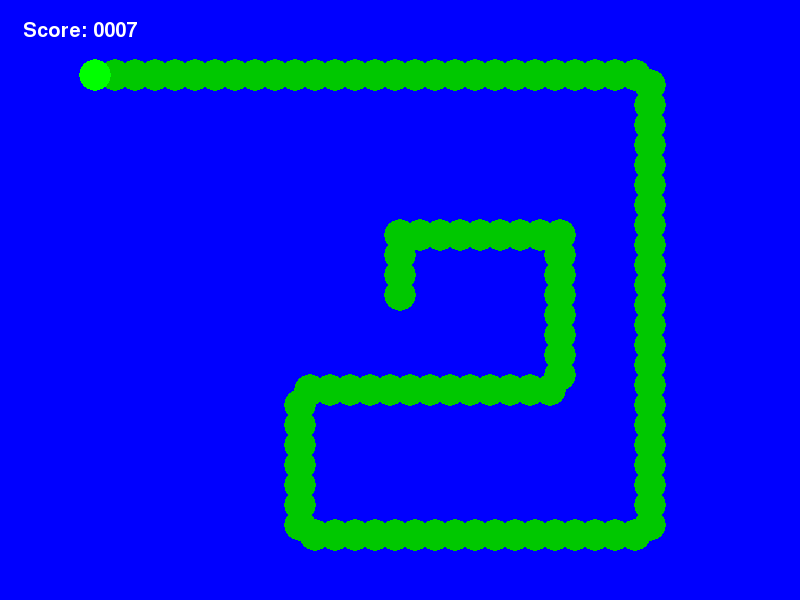
\includegraphics{ss-1-polish.png}
Ok, let's take a bit of time polish things up a bit here with a number of changes.
\begin{itemize}
\item {} 
Add a background to the display

\item {} 
Allow the user to press ESCAPE to quit the game at any time

\item {} 
Kill the snake if it goes off the screen

\item {} 
Keep score of how long the user survived

\end{itemize}

\begin{Verbatim}[commandchars=\\\{\},numbers=left,firstnumber=1,stepnumber=1]
\PYG{k+kn}{import} \PYG{n+nn}{pygame}

\PYG{k+kn}{import} \PYG{n+nn}{serge.engine}
\PYG{k+kn}{import} \PYG{n+nn}{serge.actor}
\PYG{k+kn}{import} \PYG{n+nn}{serge.blocks.visualblocks}
\PYG{k+kn}{import} \PYG{n+nn}{serge.blocks.utils}
\PYG{k+kn}{import} \PYG{n+nn}{serge.blocks.directions}
\PYG{k+kn}{import} \PYG{n+nn}{serge.blocks.behaviours}
\PYG{k+kn}{import} \PYG{n+nn}{serge.blocks.actors}

\PYG{k}{class} \PYG{n+nc}{Snake}\PYG{p}{(}\PYG{n}{serge}\PYG{o}{.}\PYG{n}{actor}\PYG{o}{.}\PYG{n}{CompositeActor}\PYG{p}{)}\PYG{p}{:}
    \PYG{l+s+sd}{"""Represents the snake"""}

    \PYG{k}{def} \PYG{n+nf}{\PYGZus{}\PYGZus{}init\PYGZus{}\PYGZus{}}\PYG{p}{(}\PYG{n+nb+bp}{self}\PYG{p}{)}\PYG{p}{:}
        \PYG{l+s+sd}{"""Initialise the snake"""}
        \PYG{n+nb}{super}\PYG{p}{(}\PYG{n}{Snake}\PYG{p}{,} \PYG{n+nb+bp}{self}\PYG{p}{)}\PYG{o}{.}\PYG{n}{\PYGZus{}\PYGZus{}init\PYGZus{}\PYGZus{}}\PYG{p}{(}\PYG{l+s}{'}\PYG{l+s}{snake}\PYG{l+s}{'}\PYG{p}{,} \PYG{l+s}{'}\PYG{l+s}{snake-head}\PYG{l+s}{'}\PYG{p}{)}
        \PYG{n+nb+bp}{self}\PYG{o}{.}\PYG{n}{visual} \PYG{o}{=} \PYG{n}{serge}\PYG{o}{.}\PYG{n}{blocks}\PYG{o}{.}\PYG{n}{visualblocks}\PYG{o}{.}\PYG{n}{Circle}\PYG{p}{(}\PYG{l+m+mi}{16}\PYG{p}{,} \PYG{p}{(}\PYG{l+m+mi}{0}\PYG{p}{,}\PYG{l+m+mi}{255}\PYG{p}{,}\PYG{l+m+mi}{0}\PYG{p}{)}\PYG{p}{)}
        \PYG{n+nb+bp}{self}\PYG{o}{.}\PYG{n}{setLayerName}\PYG{p}{(}\PYG{l+s}{'}\PYG{l+s}{middle}\PYG{l+s}{'}\PYG{p}{)}
        \PYG{n+nb+bp}{self}\PYG{o}{.}\PYG{n}{current\PYGZus{}direction} \PYG{o}{=} \PYG{n}{serge}\PYG{o}{.}\PYG{n}{blocks}\PYG{o}{.}\PYG{n}{directions}\PYG{o}{.}\PYG{n}{N}
        \PYG{n+nb+bp}{self}\PYG{o}{.}\PYG{n}{is\PYGZus{}dying} \PYG{o}{=} \PYG{n+nb+bp}{False}

    \PYG{k}{def} \PYG{n+nf}{addedToWorld}\PYG{p}{(}\PYG{n+nb+bp}{self}\PYG{p}{,} \PYG{n}{world}\PYG{p}{)}\PYG{p}{:}
        \PYG{l+s+sd}{"""The snake was added to the world"""}
        \PYG{n+nb}{super}\PYG{p}{(}\PYG{n}{Snake}\PYG{p}{,} \PYG{n+nb+bp}{self}\PYG{p}{)}\PYG{o}{.}\PYG{n}{addedToWorld}\PYG{p}{(}\PYG{n}{world}\PYG{p}{)}
        \PYG{c}{\PYGZsh{}}
        \PYG{n+nb+bp}{self}\PYG{o}{.}\PYG{n}{keyboard} \PYG{o}{=} \PYG{n}{serge}\PYG{o}{.}\PYG{n}{engine}\PYG{o}{.}\PYG{n}{CurrentEngine}\PYG{p}{(}\PYG{p}{)}\PYG{o}{.}\PYG{n}{getKeyboard}\PYG{p}{(}\PYG{p}{)}
        \PYG{n+nb+bp}{self}\PYG{o}{.}\PYG{n}{manager} \PYG{o}{=} \PYG{n}{serge}\PYG{o}{.}\PYG{n}{blocks}\PYG{o}{.}\PYG{n}{behaviours}\PYG{o}{.}\PYG{n}{BehaviourManager}\PYG{p}{(}\PYG{l+s}{'}\PYG{l+s}{manager}\PYG{l+s}{'}\PYG{p}{,} \PYG{l+s}{'}\PYG{l+s}{behaviour-manager}\PYG{l+s}{'}\PYG{p}{)}
        \PYG{n}{world}\PYG{o}{.}\PYG{n}{addActor}\PYG{p}{(}\PYG{n+nb+bp}{self}\PYG{o}{.}\PYG{n}{manager}\PYG{p}{)}
        \PYG{c}{\PYGZsh{}}
        \PYG{c}{\PYGZsh{} Text to display when the game is over}
        \PYG{n+nb+bp}{self}\PYG{o}{.}\PYG{n}{restart\PYGZus{}text} \PYG{o}{=} \PYG{n}{serge}\PYG{o}{.}\PYG{n}{blocks}\PYG{o}{.}\PYG{n}{utils}\PYG{o}{.}\PYG{n}{addVisualActorToWorld}\PYG{p}{(}\PYG{n}{world}\PYG{p}{,} \PYG{l+s}{'}\PYG{l+s}{text}\PYG{l+s}{'}\PYG{p}{,} \PYG{l+s}{'}\PYG{l+s}{restart}\PYG{l+s}{'}\PYG{p}{,}
            \PYG{n}{serge}\PYG{o}{.}\PYG{n}{visual}\PYG{o}{.}\PYG{n}{Text}\PYG{p}{(}\PYG{l+s}{'}\PYG{l+s}{Game Over - Press ENTER to restart}\PYG{l+s}{'}\PYG{p}{,} \PYG{p}{(}\PYG{l+m+mi}{255}\PYG{p}{,} \PYG{l+m+mi}{255}\PYG{p}{,} \PYG{l+m+mi}{255}\PYG{p}{)}\PYG{p}{,} \PYG{n}{font\PYGZus{}size}\PYG{o}{=}\PYG{l+m+mi}{20}\PYG{p}{)}\PYG{p}{,}
            \PYG{n}{layer\PYGZus{}name}\PYG{o}{=}\PYG{l+s}{'}\PYG{l+s}{front}\PYG{l+s}{'}\PYG{p}{,}
            \PYG{n}{center\PYGZus{}position}\PYG{o}{=}\PYG{p}{(}\PYG{l+m+mi}{400}\PYG{p}{,} \PYG{l+m+mi}{300}\PYG{p}{)}\PYG{p}{)}
        \PYG{n+nb+bp}{self}\PYG{o}{.}\PYG{n}{restart\PYGZus{}text}\PYG{o}{.}\PYG{n}{visible} \PYG{o}{=} \PYG{n+nb+bp}{False}
        \PYG{c}{\PYGZsh{}}
        \PYG{c}{\PYGZsh{} A background for the game}
        \PYG{n+nb+bp}{self}\PYG{o}{.}\PYG{n}{bg} \PYG{o}{=} \PYG{n}{serge}\PYG{o}{.}\PYG{n}{blocks}\PYG{o}{.}\PYG{n}{utils}\PYG{o}{.}\PYG{n}{addVisualActorToWorld}\PYG{p}{(}\PYG{n}{world}\PYG{p}{,} \PYG{l+s}{'}\PYG{l+s}{bg}\PYG{l+s}{'}\PYG{p}{,} \PYG{l+s}{'}\PYG{l+s}{bg}\PYG{l+s}{'}\PYG{p}{,}
            \PYG{n}{serge}\PYG{o}{.}\PYG{n}{blocks}\PYG{o}{.}\PYG{n}{visualblocks}\PYG{o}{.}\PYG{n}{Rectangle}\PYG{p}{(}\PYG{p}{(}\PYG{l+m+mi}{800}\PYG{p}{,} \PYG{l+m+mi}{600}\PYG{p}{)}\PYG{p}{,} \PYG{p}{(}\PYG{l+m+mi}{0}\PYG{p}{,}\PYG{l+m+mi}{0}\PYG{p}{,}\PYG{l+m+mi}{255}\PYG{p}{)}\PYG{p}{)}\PYG{p}{,}
            \PYG{n}{layer\PYGZus{}name}\PYG{o}{=}\PYG{l+s}{'}\PYG{l+s}{back}\PYG{l+s}{'}\PYG{p}{,}
            \PYG{n}{center\PYGZus{}position}\PYG{o}{=}\PYG{p}{(}\PYG{l+m+mi}{400}\PYG{p}{,} \PYG{l+m+mi}{300}\PYG{p}{)}\PYG{p}{)}
        \PYG{c}{\PYGZsh{}}
        \PYG{c}{\PYGZsh{} Text to show the score}
        \PYG{n+nb+bp}{self}\PYG{o}{.}\PYG{n}{score} \PYG{o}{=} \PYG{n}{serge}\PYG{o}{.}\PYG{n}{blocks}\PYG{o}{.}\PYG{n}{utils}\PYG{o}{.}\PYG{n}{addActorToWorld}\PYG{p}{(}\PYG{n}{world}\PYG{p}{,}
            \PYG{n}{serge}\PYG{o}{.}\PYG{n}{blocks}\PYG{o}{.}\PYG{n}{actors}\PYG{o}{.}\PYG{n}{NumericText}\PYG{p}{(}\PYG{l+s}{'}\PYG{l+s}{text}\PYG{l+s}{'}\PYG{p}{,} \PYG{l+s}{'}\PYG{l+s}{score}\PYG{l+s}{'}\PYG{p}{,} \PYG{l+s}{'}\PYG{l+s}{Score: }\PYG{l+s+si}{\PYGZpc{}04d}\PYG{l+s}{'}\PYG{p}{,}
                \PYG{p}{(}\PYG{l+m+mi}{255}\PYG{p}{,} \PYG{l+m+mi}{255}\PYG{p}{,} \PYG{l+m+mi}{255}\PYG{p}{)}\PYG{p}{,} \PYG{n}{font\PYGZus{}size}\PYG{o}{=}\PYG{l+m+mi}{20}\PYG{p}{,} \PYG{n}{value}\PYG{o}{=}\PYG{l+m+mi}{0}\PYG{p}{,} \PYG{n}{align}\PYG{o}{=}\PYG{l+s}{'}\PYG{l+s}{left}\PYG{l+s}{'}\PYG{p}{)}\PYG{p}{,}
            \PYG{n}{layer\PYGZus{}name}\PYG{o}{=}\PYG{l+s}{'}\PYG{l+s}{front}\PYG{l+s}{'}\PYG{p}{,}
            \PYG{n}{center\PYGZus{}position}\PYG{o}{=}\PYG{p}{(}\PYG{l+m+mi}{80}\PYG{p}{,} \PYG{l+m+mi}{30}\PYG{p}{)}\PYG{p}{)}

    \PYG{k}{def} \PYG{n+nf}{updateActor}\PYG{p}{(}\PYG{n+nb+bp}{self}\PYG{p}{,} \PYG{n}{interval}\PYG{p}{,} \PYG{n}{world}\PYG{p}{)}\PYG{p}{:}
        \PYG{l+s+sd}{"""Update the snake"""}
        \PYG{n+nb}{super}\PYG{p}{(}\PYG{n}{Snake}\PYG{p}{,} \PYG{n+nb+bp}{self}\PYG{p}{)}\PYG{o}{.}\PYG{n}{updateActor}\PYG{p}{(}\PYG{n}{interval}\PYG{p}{,} \PYG{n}{world}\PYG{p}{)}
        \PYG{c}{\PYGZsh{}}
        \PYG{c}{\PYGZsh{} Quit if requested}
        \PYG{k}{if} \PYG{n+nb+bp}{self}\PYG{o}{.}\PYG{n}{keyboard}\PYG{o}{.}\PYG{n}{isClicked}\PYG{p}{(}\PYG{n}{pygame}\PYG{o}{.}\PYG{n}{K\PYGZus{}ESCAPE}\PYG{p}{)}\PYG{p}{:}
            \PYG{n}{serge}\PYG{o}{.}\PYG{n}{engine}\PYG{o}{.}\PYG{n}{CurrentEngine}\PYG{p}{(}\PYG{p}{)}\PYG{o}{.}\PYG{n}{stop}\PYG{p}{(}\PYG{p}{)}
        \PYG{c}{\PYGZsh{}}
        \PYG{c}{\PYGZsh{} Move the head}
        \PYG{k}{if} \PYG{n+nb+bp}{self}\PYG{o}{.}\PYG{n}{keyboard}\PYG{o}{.}\PYG{n}{isClicked}\PYG{p}{(}\PYG{n}{pygame}\PYG{o}{.}\PYG{n}{K\PYGZus{}LEFT}\PYG{p}{)}\PYG{p}{:}
            \PYG{n}{rotation} \PYG{o}{=} \PYG{o}{+}\PYG{l+m+mi}{90}
        \PYG{k}{elif} \PYG{n+nb+bp}{self}\PYG{o}{.}\PYG{n}{keyboard}\PYG{o}{.}\PYG{n}{isClicked}\PYG{p}{(}\PYG{n}{pygame}\PYG{o}{.}\PYG{n}{K\PYGZus{}RIGHT}\PYG{p}{)}\PYG{p}{:}
            \PYG{n}{rotation} \PYG{o}{=} \PYG{o}{-}\PYG{l+m+mi}{90}
        \PYG{k}{else}\PYG{p}{:}
            \PYG{n}{rotation} \PYG{o}{=} \PYG{l+m+mi}{0}
        \PYG{c}{\PYGZsh{}}
        \PYG{c}{\PYGZsh{} Change direction}
        \PYG{k}{if} \PYG{n}{rotation}\PYG{p}{:}
            \PYG{n}{current\PYGZus{}angle} \PYG{o}{=} \PYG{n}{serge}\PYG{o}{.}\PYG{n}{blocks}\PYG{o}{.}\PYG{n}{directions}\PYG{o}{.}\PYG{n}{getAngleFromCardinal}\PYG{p}{(}\PYG{n+nb+bp}{self}\PYG{o}{.}\PYG{n}{current\PYGZus{}direction}\PYG{p}{)}
            \PYG{n+nb+bp}{self}\PYG{o}{.}\PYG{n}{current\PYGZus{}direction} \PYG{o}{=} \PYG{n}{serge}\PYG{o}{.}\PYG{n}{blocks}\PYG{o}{.}\PYG{n}{directions}\PYG{o}{.}\PYG{n}{getCardinalFromAngle}\PYG{p}{(}\PYG{n}{current\PYGZus{}angle}\PYG{o}{+}\PYG{n}{rotation}\PYG{p}{)}
        \PYG{c}{\PYGZsh{}}
        \PYG{c}{\PYGZsh{} Move}
        \PYG{k}{if} \PYG{o+ow}{not} \PYG{n+nb+bp}{self}\PYG{o}{.}\PYG{n}{is\PYGZus{}dying}\PYG{p}{:}
            \PYG{n}{offset} \PYG{o}{=} \PYG{l+m+mi}{5}\PYG{o}{*}\PYG{n}{serge}\PYG{o}{.}\PYG{n}{blocks}\PYG{o}{.}\PYG{n}{directions}\PYG{o}{.}\PYG{n}{getVectorFromCardinal}\PYG{p}{(}\PYG{n+nb+bp}{self}\PYG{o}{.}\PYG{n}{current\PYGZus{}direction}\PYG{p}{)}
            \PYG{n+nb+bp}{self}\PYG{o}{.}\PYG{n}{move}\PYG{p}{(}\PYG{o}{*}\PYG{n}{offset}\PYG{p}{)}
            \PYG{c}{\PYGZsh{}}
            \PYG{c}{\PYGZsh{} Add a new segment if needed}
            \PYG{k}{if} \PYG{o+ow}{not} \PYG{n+nb+bp}{self}\PYG{o}{.}\PYG{n}{getChildren}\PYG{p}{(}\PYG{p}{)} \PYG{o+ow}{or} \PYG{n+nb+bp}{self}\PYG{o}{.}\PYG{n}{getDistanceFrom}\PYG{p}{(}\PYG{n+nb+bp}{self}\PYG{o}{.}\PYG{n}{getChildren}\PYG{p}{(}\PYG{p}{)}\PYG{p}{[}\PYG{o}{-}\PYG{l+m+mi}{1}\PYG{p}{]}\PYG{p}{)} \PYG{o}{\textgreater{}} \PYG{l+m+mi}{16}\PYG{p}{:}
                \PYG{n+nb+bp}{self}\PYG{o}{.}\PYG{n}{addSegment}\PYG{p}{(}\PYG{p}{)}
            \PYG{c}{\PYGZsh{}}
            \PYG{c}{\PYGZsh{} Check if we hit the body}
            \PYG{k}{if} \PYG{n+nb+bp}{self}\PYG{o}{.}\PYG{n}{hitBody}\PYG{p}{(}\PYG{p}{)} \PYG{o+ow}{or} \PYG{n+nb+bp}{self}\PYG{o}{.}\PYG{n}{offScreen}\PYG{p}{(}\PYG{p}{)}\PYG{p}{:}
                \PYG{n+nb+bp}{self}\PYG{o}{.}\PYG{n}{initiateDeathAnimation}\PYG{p}{(}\PYG{p}{)}
            \PYG{c}{\PYGZsh{}}
            \PYG{c}{\PYGZsh{} Increase score}
            \PYG{n+nb+bp}{self}\PYG{o}{.}\PYG{n}{score}\PYG{o}{.}\PYG{n}{value} \PYG{o}{+}\PYG{o}{=} \PYG{n}{interval}\PYG{o}{/}\PYG{l+m+mf}{1000.0}
        \PYG{k}{elif} \PYG{n+nb+bp}{self}\PYG{o}{.}\PYG{n}{animation}\PYG{o}{.}\PYG{n}{isComplete}\PYG{p}{(}\PYG{p}{)}\PYG{p}{:}
            \PYG{k}{if} \PYG{n+nb+bp}{self}\PYG{o}{.}\PYG{n}{keyboard}\PYG{o}{.}\PYG{n}{isClicked}\PYG{p}{(}\PYG{n}{pygame}\PYG{o}{.}\PYG{n}{K\PYGZus{}KP\PYGZus{}ENTER}\PYG{p}{)} \PYG{o+ow}{or} \PYG{n+nb+bp}{self}\PYG{o}{.}\PYG{n}{keyboard}\PYG{o}{.}\PYG{n}{isClicked}\PYG{p}{(}\PYG{n}{pygame}\PYG{o}{.}\PYG{n}{K\PYGZus{}RETURN}\PYG{p}{)}\PYG{p}{:}
                \PYG{n+nb+bp}{self}\PYG{o}{.}\PYG{n}{restartGame}\PYG{p}{(}\PYG{p}{)}

    \PYG{k}{def} \PYG{n+nf}{addSegment}\PYG{p}{(}\PYG{n+nb+bp}{self}\PYG{p}{)}\PYG{p}{:}
        \PYG{l+s+sd}{"""Add a new body segment"""}
        \PYG{n}{segment} \PYG{o}{=} \PYG{n}{serge}\PYG{o}{.}\PYG{n}{actor}\PYG{o}{.}\PYG{n}{Actor}\PYG{p}{(}\PYG{l+s}{'}\PYG{l+s}{segment}\PYG{l+s}{'}\PYG{p}{)}
        \PYG{n}{segment}\PYG{o}{.}\PYG{n}{visual} \PYG{o}{=} \PYG{n}{serge}\PYG{o}{.}\PYG{n}{blocks}\PYG{o}{.}\PYG{n}{visualblocks}\PYG{o}{.}\PYG{n}{Circle}\PYG{p}{(}\PYG{l+m+mi}{16}\PYG{p}{,} \PYG{p}{(}\PYG{l+m+mi}{0}\PYG{p}{,}\PYG{l+m+mi}{200}\PYG{p}{,}\PYG{l+m+mi}{0}\PYG{p}{)}\PYG{p}{)}
        \PYG{n}{segment}\PYG{o}{.}\PYG{n}{setLayerName}\PYG{p}{(}\PYG{l+s}{'}\PYG{l+s}{middle}\PYG{l+s}{'}\PYG{p}{)}
        \PYG{n}{segment}\PYG{o}{.}\PYG{n}{moveTo}\PYG{p}{(}\PYG{n+nb+bp}{self}\PYG{o}{.}\PYG{n}{x}\PYG{p}{,} \PYG{n+nb+bp}{self}\PYG{o}{.}\PYG{n}{y}\PYG{p}{)}
        \PYG{n+nb+bp}{self}\PYG{o}{.}\PYG{n}{addChild}\PYG{p}{(}\PYG{n}{segment}\PYG{p}{)}

    \PYG{k}{def} \PYG{n+nf}{hitBody}\PYG{p}{(}\PYG{n+nb+bp}{self}\PYG{p}{)}\PYG{p}{:}
        \PYG{l+s+sd}{"""Return True if the head has hit the body}

\PYG{l+s+sd}{        Look to see if we overlap with any body segment except the last}
\PYG{l+s+sd}{        (we are allowed to overlap the last since we just put it down)}

\PYG{l+s+sd}{        """}
        \PYG{k}{for} \PYG{n}{segment} \PYG{o+ow}{in} \PYG{n+nb+bp}{self}\PYG{o}{.}\PYG{n}{getChildren}\PYG{p}{(}\PYG{p}{)}\PYG{p}{[}\PYG{p}{:}\PYG{o}{-}\PYG{l+m+mi}{1}\PYG{p}{]}\PYG{p}{:}
            \PYG{k}{if} \PYG{n+nb+bp}{self}\PYG{o}{.}\PYG{n}{getDistanceFrom}\PYG{p}{(}\PYG{n}{segment}\PYG{p}{)} \PYG{o}{\textless{}} \PYG{l+m+mi}{16}\PYG{p}{:}
                \PYG{k}{return} \PYG{n+nb+bp}{True}
        \PYG{k}{return} \PYG{n+nb+bp}{False}

    \PYG{k}{def} \PYG{n+nf}{offScreen}\PYG{p}{(}\PYG{n+nb+bp}{self}\PYG{p}{)}\PYG{p}{:}
        \PYG{l+s+sd}{"""Return True if we are off the screen"""}
        \PYG{k}{return} \PYG{n+nb+bp}{self}\PYG{o}{.}\PYG{n}{x} \PYG{o}{\textless{}} \PYG{l+m+mi}{0} \PYG{o+ow}{or} \PYG{n+nb+bp}{self}\PYG{o}{.}\PYG{n}{x} \PYG{o}{\textgreater{}} \PYG{l+m+mi}{800} \PYG{o+ow}{or} \PYG{n+nb+bp}{self}\PYG{o}{.}\PYG{n}{y} \PYG{o}{\textless{}} \PYG{l+m+mi}{0} \PYG{o+ow}{or} \PYG{n+nb+bp}{self}\PYG{o}{.}\PYG{n}{y} \PYG{o}{\textgreater{}} \PYG{l+m+mi}{600}

    \PYG{k}{def} \PYG{n+nf}{initiateDeathAnimation}\PYG{p}{(}\PYG{n+nb+bp}{self}\PYG{p}{)}\PYG{p}{:}
        \PYG{l+s+sd}{"""Begin showing the death of the snake"""}
        \PYG{n+nb+bp}{self}\PYG{o}{.}\PYG{n}{log}\PYG{o}{.}\PYG{n}{info}\PYG{p}{(}\PYG{l+s}{'}\PYG{l+s}{Snake died!}\PYG{l+s}{'}\PYG{p}{)}
        \PYG{n+nb+bp}{self}\PYG{o}{.}\PYG{n}{animation} \PYG{o}{=} \PYG{n+nb+bp}{self}\PYG{o}{.}\PYG{n}{manager}\PYG{o}{.}\PYG{n}{assignBehaviour}\PYG{p}{(}\PYG{n+nb+bp}{self}\PYG{p}{,}
            \PYG{n}{serge}\PYG{o}{.}\PYG{n}{blocks}\PYG{o}{.}\PYG{n}{behaviours}\PYG{o}{.}\PYG{n}{TimedCallback}\PYG{p}{(}\PYG{l+m+mi}{1000}\PYG{o}{/}\PYG{n+nb}{len}\PYG{p}{(}\PYG{n+nb+bp}{self}\PYG{o}{.}\PYG{n}{getChildren}\PYG{p}{(}\PYG{p}{)}\PYG{p}{)}\PYG{p}{,} \PYG{n+nb+bp}{self}\PYG{o}{.}\PYG{n}{removeTail}\PYG{p}{)}\PYG{p}{,} \PYG{l+s}{'}\PYG{l+s}{death-animation}\PYG{l+s}{'}\PYG{p}{)}
        \PYG{n+nb+bp}{self}\PYG{o}{.}\PYG{n}{is\PYGZus{}dying} \PYG{o}{=} \PYG{n+nb+bp}{True}
        \PYG{k}{for} \PYG{n}{segment} \PYG{o+ow}{in} \PYG{n+nb+bp}{self}\PYG{o}{.}\PYG{n}{getChildren}\PYG{p}{(}\PYG{p}{)}\PYG{p}{:}
            \PYG{n}{segment}\PYG{o}{.}\PYG{n}{visual}\PYG{o}{.}\PYG{n}{colour} \PYG{o}{=} \PYG{p}{(}\PYG{l+m+mi}{200}\PYG{p}{,} \PYG{l+m+mi}{0}\PYG{p}{,} \PYG{l+m+mi}{0}\PYG{p}{)}
        \PYG{n+nb+bp}{self}\PYG{o}{.}\PYG{n}{visual}\PYG{o}{.}\PYG{n}{colour} \PYG{o}{=} \PYG{p}{(}\PYG{l+m+mi}{255}\PYG{p}{,} \PYG{l+m+mi}{0}\PYG{p}{,} \PYG{l+m+mi}{0}\PYG{p}{)}

    \PYG{k}{def} \PYG{n+nf}{removeTail}\PYG{p}{(}\PYG{n+nb+bp}{self}\PYG{p}{,} \PYG{n}{world}\PYG{p}{,} \PYG{n}{actor}\PYG{p}{,} \PYG{n}{interval}\PYG{p}{)}\PYG{p}{:}
        \PYG{l+s+sd}{"""Remove part of the tail"""}
        \PYG{n+nb+bp}{self}\PYG{o}{.}\PYG{n}{log}\PYG{o}{.}\PYG{n}{debug}\PYG{p}{(}\PYG{l+s}{'}\PYG{l+s}{Removing part of the tail}\PYG{l+s}{'}\PYG{p}{)}
        \PYG{k}{if} \PYG{n+nb+bp}{self}\PYG{o}{.}\PYG{n}{getChildren}\PYG{p}{(}\PYG{p}{)}\PYG{p}{:}
            \PYG{n+nb+bp}{self}\PYG{o}{.}\PYG{n}{removeChild}\PYG{p}{(}\PYG{n+nb+bp}{self}\PYG{o}{.}\PYG{n}{getChildren}\PYG{p}{(}\PYG{p}{)}\PYG{p}{[}\PYG{l+m+mi}{0}\PYG{p}{]}\PYG{p}{)}
        \PYG{k}{else}\PYG{p}{:}
            \PYG{n+nb+bp}{self}\PYG{o}{.}\PYG{n}{animation}\PYG{o}{.}\PYG{n}{markComplete}\PYG{p}{(}\PYG{p}{)}
            \PYG{n+nb+bp}{self}\PYG{o}{.}\PYG{n}{restart\PYGZus{}text}\PYG{o}{.}\PYG{n}{visible} \PYG{o}{=} \PYG{n+nb+bp}{True}

    \PYG{k}{def} \PYG{n+nf}{restartGame}\PYG{p}{(}\PYG{n+nb+bp}{self}\PYG{p}{)}\PYG{p}{:}
        \PYG{l+s+sd}{"""Restart the game"""}
        \PYG{n+nb+bp}{self}\PYG{o}{.}\PYG{n}{is\PYGZus{}dying} \PYG{o}{=} \PYG{n+nb+bp}{False}
        \PYG{n+nb+bp}{self}\PYG{o}{.}\PYG{n}{restart\PYGZus{}text}\PYG{o}{.}\PYG{n}{visible} \PYG{o}{=} \PYG{n+nb+bp}{False}
        \PYG{n+nb+bp}{self}\PYG{o}{.}\PYG{n}{visual}\PYG{o}{.}\PYG{n}{colour} \PYG{o}{=} \PYG{p}{(}\PYG{l+m+mi}{0}\PYG{p}{,}\PYG{l+m+mi}{255}\PYG{p}{,}\PYG{l+m+mi}{0}\PYG{p}{)}
        \PYG{n+nb+bp}{self}\PYG{o}{.}\PYG{n}{current\PYGZus{}direction} \PYG{o}{=} \PYG{n}{serge}\PYG{o}{.}\PYG{n}{blocks}\PYG{o}{.}\PYG{n}{directions}\PYG{o}{.}\PYG{n}{N}
        \PYG{n+nb+bp}{self}\PYG{o}{.}\PYG{n}{score}\PYG{o}{.}\PYG{n}{value} \PYG{o}{=} \PYG{l+m+mi}{0}
        \PYG{n+nb+bp}{self}\PYG{o}{.}\PYG{n}{moveTo}\PYG{p}{(}\PYG{l+m+mi}{400}\PYG{p}{,} \PYG{l+m+mi}{300}\PYG{p}{)}

\PYG{c}{\PYGZsh{} Create the engine}
\PYG{n}{engine} \PYG{o}{=} \PYG{n}{serge}\PYG{o}{.}\PYG{n}{blocks}\PYG{o}{.}\PYG{n}{utils}\PYG{o}{.}\PYG{n}{getSimpleSetup}\PYG{p}{(}\PYG{l+m+mi}{800}\PYG{p}{,} \PYG{l+m+mi}{600}\PYG{p}{)}
\PYG{n}{world} \PYG{o}{=} \PYG{n}{engine}\PYG{o}{.}\PYG{n}{getWorld}\PYG{p}{(}\PYG{l+s}{'}\PYG{l+s}{lab}\PYG{l+s}{'}\PYG{p}{)}

\PYG{c}{\PYGZsh{} Create the snake}
\PYG{n}{snake} \PYG{o}{=} \PYG{n}{Snake}\PYG{p}{(}\PYG{p}{)}
\PYG{n}{world}\PYG{o}{.}\PYG{n}{addActor}\PYG{p}{(}\PYG{n}{snake}\PYG{p}{)}
\PYG{n}{snake}\PYG{o}{.}\PYG{n}{moveTo}\PYG{p}{(}\PYG{l+m+mi}{400}\PYG{p}{,} \PYG{l+m+mi}{300}\PYG{p}{)}

\PYG{c}{\PYGZsh{} Run the game}
\PYG{n}{engine}\PYG{o}{.}\PYG{n}{run}\PYG{p}{(}\PYG{l+m+mi}{60}\PYG{p}{)}
\end{Verbatim}

This tutorial continues in {\hyperref[tutorial-2::doc]{\emph{Tutorial 2: Snake Part 2}}}.


\section{Tutorial 2: Snake Part 2}
\label{tutorial-2:tutorial-2-snake-part-2}\label{tutorial-2::doc}\setbox0\vbox{
\begin{minipage}{0.95\linewidth}
\textbf{Contents}

\medskip

\begin{itemize}
\item {} 
{\hyperref[tutorial-2:tutorial-2-snake-part-2]{Tutorial 2: Snake Part 2}}
\begin{itemize}
\item {} 
{\hyperref[tutorial-2:adding-sprites]{Adding Sprites}}

\item {} 
{\hyperref[tutorial-2:adding-sound]{Adding Sound}}

\item {} 
{\hyperref[tutorial-2:adding-fonts]{Adding Fonts}}

\item {} 
{\hyperref[tutorial-2:additional-gameplay-elements]{Additional Gameplay elements}}

\item {} 
{\hyperref[tutorial-2:events]{Events}}

\item {} 
{\hyperref[tutorial-2:animation]{Animation}}

\item {} 
{\hyperref[tutorial-2:conclusion]{Conclusion}}

\item {} 
{\hyperref[tutorial-2:resources]{Resources}}

\item {} 
{\hyperref[tutorial-2:credits]{Credits}}

\end{itemize}

\end{itemize}
\end{minipage}}
\begin{center}\setlength{\fboxsep}{5pt}\shadowbox{\box0}\end{center}

This tutorial continues on from {\hyperref[tutorial-1::doc]{\emph{Tutorial 1: Snake Part 1}}}.

The basic game is in place and we will now add sprites, sound, fonts, animation and events.


\subsection{Adding Sprites}
\label{tutorial-2:adding-sprites}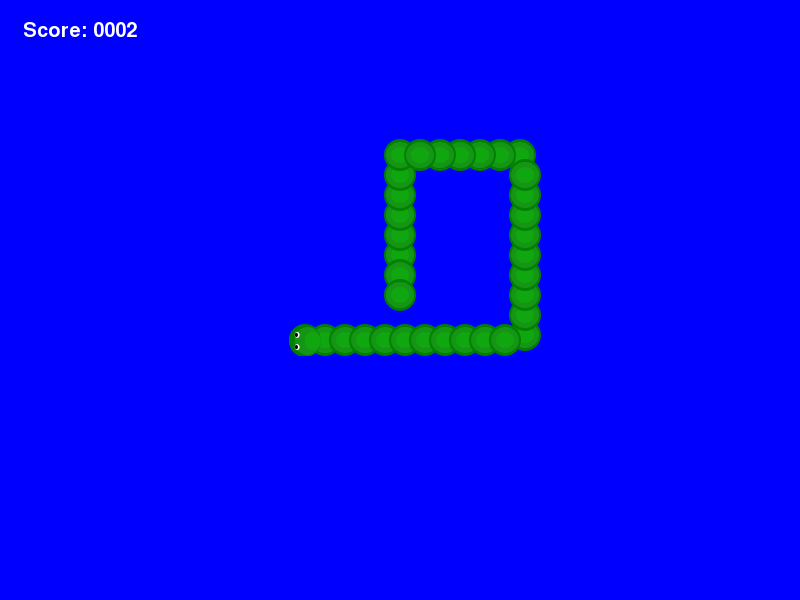
\includegraphics{ss-1-sprites.png}
The game is working ok but we need to add some sprites to start to make it look like a
real game. We will add a sprite for the head and one for the body.

To use sprites with serge you first need to register them in the sprite registry. You can
create simple sprites and animated sprites from single files (sprite sheets) or multiple
files. For the moment let's just stick with simple sprites.

To register a sprite you use code like this.

\begin{Verbatim}[commandchars=\\\{\},numbers=left,firstnumber=1,stepnumber=1]
\PYG{k+kn}{import} \PYG{n+nn}{serge.visual}
\PYG{n}{serge}\PYG{o}{.}\PYG{n}{visual}\PYG{o}{.}\PYG{n}{Sprites}\PYG{o}{.}\PYG{n}{setPath}\PYG{p}{(}\PYG{l+s}{'}\PYG{l+s}{graphics}\PYG{l+s}{'}\PYG{p}{)}
\PYG{n}{serge}\PYG{o}{.}\PYG{n}{visual}\PYG{o}{.}\PYG{n}{Sprites}\PYG{o}{.}\PYG{n}{registerItem}\PYG{p}{(}\PYG{l+s}{'}\PYG{l+s}{head}\PYG{l+s}{'}\PYG{p}{,} \PYG{l+s}{'}\PYG{l+s}{head.png}\PYG{l+s}{'}\PYG{p}{)}
\PYG{n}{serge}\PYG{o}{.}\PYG{n}{visual}\PYG{o}{.}\PYG{n}{Sprites}\PYG{o}{.}\PYG{n}{registerItem}\PYG{p}{(}\PYG{l+s}{'}\PYG{l+s}{tail}\PYG{l+s}{'}\PYG{p}{,} \PYG{l+s}{'}\PYG{l+s}{tail.png}\PYG{l+s}{'}\PYG{p}{)}
\end{Verbatim}

It is best to put all sprites in a separate folder. You then use \emph{setPath} to point serge
at the folder. Then you make repeated calls to \emph{registerItem} to register each sprite. You
give the sprite a name and the file that you want to use.

Once you have registered a sprite you then use it for an actor's visual by calling the \emph{setSpriteName}
method of the actor. For example.

\begin{Verbatim}[commandchars=\\\{\},numbers=left,firstnumber=1,stepnumber=1]
\PYG{n}{snake}\PYG{o}{.}\PYG{n}{setSpriteName}\PYG{p}{(}\PYG{l+s}{'}\PYG{l+s}{head}\PYG{l+s}{'}\PYG{p}{)}
\end{Verbatim}

Now the head sprite will be used.

Let's add that to our code now. You can download the graphics here (zipfile).

\begin{Verbatim}[commandchars=\\\{\},numbers=left,firstnumber=1,stepnumber=1]
\PYG{k+kn}{import} \PYG{n+nn}{pygame}

\PYG{k+kn}{import} \PYG{n+nn}{serge.visual}
\PYG{k+kn}{import} \PYG{n+nn}{serge.engine}
\PYG{k+kn}{import} \PYG{n+nn}{serge.actor}
\PYG{k+kn}{import} \PYG{n+nn}{serge.blocks.visualblocks}
\PYG{k+kn}{import} \PYG{n+nn}{serge.blocks.utils}
\PYG{k+kn}{import} \PYG{n+nn}{serge.blocks.directions}
\PYG{k+kn}{import} \PYG{n+nn}{serge.blocks.behaviours}
\PYG{k+kn}{import} \PYG{n+nn}{serge.blocks.actors}

\PYG{k}{class} \PYG{n+nc}{Snake}\PYG{p}{(}\PYG{n}{serge}\PYG{o}{.}\PYG{n}{actor}\PYG{o}{.}\PYG{n}{CompositeActor}\PYG{p}{)}\PYG{p}{:}
    \PYG{l+s+sd}{"""Represents the snake"""}

    \PYG{k}{def} \PYG{n+nf}{\PYGZus{}\PYGZus{}init\PYGZus{}\PYGZus{}}\PYG{p}{(}\PYG{n+nb+bp}{self}\PYG{p}{)}\PYG{p}{:}
        \PYG{l+s+sd}{"""Initialise the snake"""}
        \PYG{n+nb}{super}\PYG{p}{(}\PYG{n}{Snake}\PYG{p}{,} \PYG{n+nb+bp}{self}\PYG{p}{)}\PYG{o}{.}\PYG{n}{\PYGZus{}\PYGZus{}init\PYGZus{}\PYGZus{}}\PYG{p}{(}\PYG{l+s}{'}\PYG{l+s}{snake}\PYG{l+s}{'}\PYG{p}{,} \PYG{l+s}{'}\PYG{l+s}{snake-head}\PYG{l+s}{'}\PYG{p}{)}
        \PYG{n+nb+bp}{self}\PYG{o}{.}\PYG{n}{visual} \PYG{o}{=} \PYG{n}{serge}\PYG{o}{.}\PYG{n}{blocks}\PYG{o}{.}\PYG{n}{visualblocks}\PYG{o}{.}\PYG{n}{Circle}\PYG{p}{(}\PYG{l+m+mi}{16}\PYG{p}{,} \PYG{p}{(}\PYG{l+m+mi}{0}\PYG{p}{,}\PYG{l+m+mi}{255}\PYG{p}{,}\PYG{l+m+mi}{0}\PYG{p}{)}\PYG{p}{)}
        \PYG{n+nb+bp}{self}\PYG{o}{.}\PYG{n}{setSpriteName}\PYG{p}{(}\PYG{l+s}{'}\PYG{l+s}{head}\PYG{l+s}{'}\PYG{p}{)}
        \PYG{n+nb+bp}{self}\PYG{o}{.}\PYG{n}{setLayerName}\PYG{p}{(}\PYG{l+s}{'}\PYG{l+s}{middle}\PYG{l+s}{'}\PYG{p}{)}
        \PYG{n+nb+bp}{self}\PYG{o}{.}\PYG{n}{current\PYGZus{}direction} \PYG{o}{=} \PYG{n}{serge}\PYG{o}{.}\PYG{n}{blocks}\PYG{o}{.}\PYG{n}{directions}\PYG{o}{.}\PYG{n}{N}
        \PYG{n+nb+bp}{self}\PYG{o}{.}\PYG{n}{is\PYGZus{}dying} \PYG{o}{=} \PYG{n+nb+bp}{False}

    \PYG{k}{def} \PYG{n+nf}{addedToWorld}\PYG{p}{(}\PYG{n+nb+bp}{self}\PYG{p}{,} \PYG{n}{world}\PYG{p}{)}\PYG{p}{:}
        \PYG{l+s+sd}{"""The snake was added to the world"""}
        \PYG{n+nb}{super}\PYG{p}{(}\PYG{n}{Snake}\PYG{p}{,} \PYG{n+nb+bp}{self}\PYG{p}{)}\PYG{o}{.}\PYG{n}{addedToWorld}\PYG{p}{(}\PYG{n}{world}\PYG{p}{)}
        \PYG{c}{\PYGZsh{}}
        \PYG{n+nb+bp}{self}\PYG{o}{.}\PYG{n}{keyboard} \PYG{o}{=} \PYG{n}{serge}\PYG{o}{.}\PYG{n}{engine}\PYG{o}{.}\PYG{n}{CurrentEngine}\PYG{p}{(}\PYG{p}{)}\PYG{o}{.}\PYG{n}{getKeyboard}\PYG{p}{(}\PYG{p}{)}
        \PYG{n+nb+bp}{self}\PYG{o}{.}\PYG{n}{manager} \PYG{o}{=} \PYG{n}{serge}\PYG{o}{.}\PYG{n}{blocks}\PYG{o}{.}\PYG{n}{behaviours}\PYG{o}{.}\PYG{n}{BehaviourManager}\PYG{p}{(}\PYG{l+s}{'}\PYG{l+s}{manager}\PYG{l+s}{'}\PYG{p}{,} \PYG{l+s}{'}\PYG{l+s}{behaviour-manager}\PYG{l+s}{'}\PYG{p}{)}
        \PYG{n}{world}\PYG{o}{.}\PYG{n}{addActor}\PYG{p}{(}\PYG{n+nb+bp}{self}\PYG{o}{.}\PYG{n}{manager}\PYG{p}{)}
        \PYG{c}{\PYGZsh{}}
        \PYG{c}{\PYGZsh{} Text to display when the game is over}
        \PYG{n+nb+bp}{self}\PYG{o}{.}\PYG{n}{restart\PYGZus{}text} \PYG{o}{=} \PYG{n}{serge}\PYG{o}{.}\PYG{n}{blocks}\PYG{o}{.}\PYG{n}{utils}\PYG{o}{.}\PYG{n}{addVisualActorToWorld}\PYG{p}{(}\PYG{n}{world}\PYG{p}{,} \PYG{l+s}{'}\PYG{l+s}{text}\PYG{l+s}{'}\PYG{p}{,} \PYG{l+s}{'}\PYG{l+s}{restart}\PYG{l+s}{'}\PYG{p}{,}
            \PYG{n}{serge}\PYG{o}{.}\PYG{n}{visual}\PYG{o}{.}\PYG{n}{Text}\PYG{p}{(}\PYG{l+s}{'}\PYG{l+s}{Game Over - Press ENTER to restart}\PYG{l+s}{'}\PYG{p}{,} \PYG{p}{(}\PYG{l+m+mi}{255}\PYG{p}{,} \PYG{l+m+mi}{255}\PYG{p}{,} \PYG{l+m+mi}{255}\PYG{p}{)}\PYG{p}{,} \PYG{n}{font\PYGZus{}size}\PYG{o}{=}\PYG{l+m+mi}{20}\PYG{p}{)}\PYG{p}{,}
            \PYG{n}{layer\PYGZus{}name}\PYG{o}{=}\PYG{l+s}{'}\PYG{l+s}{front}\PYG{l+s}{'}\PYG{p}{,}
            \PYG{n}{center\PYGZus{}position}\PYG{o}{=}\PYG{p}{(}\PYG{l+m+mi}{400}\PYG{p}{,} \PYG{l+m+mi}{300}\PYG{p}{)}\PYG{p}{)}
        \PYG{n+nb+bp}{self}\PYG{o}{.}\PYG{n}{restart\PYGZus{}text}\PYG{o}{.}\PYG{n}{visible} \PYG{o}{=} \PYG{n+nb+bp}{False}
        \PYG{c}{\PYGZsh{}}
        \PYG{c}{\PYGZsh{} A background for the game}
        \PYG{n+nb+bp}{self}\PYG{o}{.}\PYG{n}{bg} \PYG{o}{=} \PYG{n}{serge}\PYG{o}{.}\PYG{n}{blocks}\PYG{o}{.}\PYG{n}{utils}\PYG{o}{.}\PYG{n}{addVisualActorToWorld}\PYG{p}{(}\PYG{n}{world}\PYG{p}{,} \PYG{l+s}{'}\PYG{l+s}{bg}\PYG{l+s}{'}\PYG{p}{,} \PYG{l+s}{'}\PYG{l+s}{bg}\PYG{l+s}{'}\PYG{p}{,}
            \PYG{n}{serge}\PYG{o}{.}\PYG{n}{blocks}\PYG{o}{.}\PYG{n}{visualblocks}\PYG{o}{.}\PYG{n}{Rectangle}\PYG{p}{(}\PYG{p}{(}\PYG{l+m+mi}{800}\PYG{p}{,} \PYG{l+m+mi}{600}\PYG{p}{)}\PYG{p}{,} \PYG{p}{(}\PYG{l+m+mi}{0}\PYG{p}{,}\PYG{l+m+mi}{0}\PYG{p}{,}\PYG{l+m+mi}{255}\PYG{p}{)}\PYG{p}{)}\PYG{p}{,}
            \PYG{n}{layer\PYGZus{}name}\PYG{o}{=}\PYG{l+s}{'}\PYG{l+s}{back}\PYG{l+s}{'}\PYG{p}{,}
            \PYG{n}{center\PYGZus{}position}\PYG{o}{=}\PYG{p}{(}\PYG{l+m+mi}{400}\PYG{p}{,} \PYG{l+m+mi}{300}\PYG{p}{)}\PYG{p}{)}
        \PYG{c}{\PYGZsh{}}
        \PYG{c}{\PYGZsh{} Text to show the score}
        \PYG{n+nb+bp}{self}\PYG{o}{.}\PYG{n}{score} \PYG{o}{=} \PYG{n}{serge}\PYG{o}{.}\PYG{n}{blocks}\PYG{o}{.}\PYG{n}{utils}\PYG{o}{.}\PYG{n}{addActorToWorld}\PYG{p}{(}\PYG{n}{world}\PYG{p}{,}
            \PYG{n}{serge}\PYG{o}{.}\PYG{n}{blocks}\PYG{o}{.}\PYG{n}{actors}\PYG{o}{.}\PYG{n}{NumericText}\PYG{p}{(}\PYG{l+s}{'}\PYG{l+s}{text}\PYG{l+s}{'}\PYG{p}{,} \PYG{l+s}{'}\PYG{l+s}{score}\PYG{l+s}{'}\PYG{p}{,} \PYG{l+s}{'}\PYG{l+s}{Score: }\PYG{l+s+si}{\PYGZpc{}04d}\PYG{l+s}{'}\PYG{p}{,}
                \PYG{p}{(}\PYG{l+m+mi}{255}\PYG{p}{,} \PYG{l+m+mi}{255}\PYG{p}{,} \PYG{l+m+mi}{255}\PYG{p}{)}\PYG{p}{,} \PYG{n}{font\PYGZus{}size}\PYG{o}{=}\PYG{l+m+mi}{20}\PYG{p}{,} \PYG{n}{value}\PYG{o}{=}\PYG{l+m+mi}{0}\PYG{p}{,} \PYG{n}{align}\PYG{o}{=}\PYG{l+s}{'}\PYG{l+s}{left}\PYG{l+s}{'}\PYG{p}{)}\PYG{p}{,}
            \PYG{n}{layer\PYGZus{}name}\PYG{o}{=}\PYG{l+s}{'}\PYG{l+s}{front}\PYG{l+s}{'}\PYG{p}{,}
            \PYG{n}{center\PYGZus{}position}\PYG{o}{=}\PYG{p}{(}\PYG{l+m+mi}{80}\PYG{p}{,} \PYG{l+m+mi}{30}\PYG{p}{)}\PYG{p}{)}

    \PYG{k}{def} \PYG{n+nf}{updateActor}\PYG{p}{(}\PYG{n+nb+bp}{self}\PYG{p}{,} \PYG{n}{interval}\PYG{p}{,} \PYG{n}{world}\PYG{p}{)}\PYG{p}{:}
        \PYG{l+s+sd}{"""Update the snake"""}
        \PYG{n+nb}{super}\PYG{p}{(}\PYG{n}{Snake}\PYG{p}{,} \PYG{n+nb+bp}{self}\PYG{p}{)}\PYG{o}{.}\PYG{n}{updateActor}\PYG{p}{(}\PYG{n}{interval}\PYG{p}{,} \PYG{n}{world}\PYG{p}{)}
        \PYG{c}{\PYGZsh{}}
        \PYG{c}{\PYGZsh{} Quit if requested}
        \PYG{k}{if} \PYG{n+nb+bp}{self}\PYG{o}{.}\PYG{n}{keyboard}\PYG{o}{.}\PYG{n}{isClicked}\PYG{p}{(}\PYG{n}{pygame}\PYG{o}{.}\PYG{n}{K\PYGZus{}ESCAPE}\PYG{p}{)}\PYG{p}{:}
            \PYG{n}{serge}\PYG{o}{.}\PYG{n}{engine}\PYG{o}{.}\PYG{n}{CurrentEngine}\PYG{p}{(}\PYG{p}{)}\PYG{o}{.}\PYG{n}{stop}\PYG{p}{(}\PYG{p}{)}
        \PYG{c}{\PYGZsh{}}
        \PYG{c}{\PYGZsh{} Move the head}
        \PYG{k}{if} \PYG{n+nb+bp}{self}\PYG{o}{.}\PYG{n}{keyboard}\PYG{o}{.}\PYG{n}{isClicked}\PYG{p}{(}\PYG{n}{pygame}\PYG{o}{.}\PYG{n}{K\PYGZus{}LEFT}\PYG{p}{)}\PYG{p}{:}
            \PYG{n}{rotation} \PYG{o}{=} \PYG{o}{+}\PYG{l+m+mi}{90}
        \PYG{k}{elif} \PYG{n+nb+bp}{self}\PYG{o}{.}\PYG{n}{keyboard}\PYG{o}{.}\PYG{n}{isClicked}\PYG{p}{(}\PYG{n}{pygame}\PYG{o}{.}\PYG{n}{K\PYGZus{}RIGHT}\PYG{p}{)}\PYG{p}{:}
            \PYG{n}{rotation} \PYG{o}{=} \PYG{o}{-}\PYG{l+m+mi}{90}
        \PYG{k}{else}\PYG{p}{:}
            \PYG{n}{rotation} \PYG{o}{=} \PYG{l+m+mi}{0}
        \PYG{c}{\PYGZsh{}}
        \PYG{c}{\PYGZsh{} Change direction}
        \PYG{k}{if} \PYG{n}{rotation}\PYG{p}{:}
            \PYG{n}{current\PYGZus{}angle} \PYG{o}{=} \PYG{n}{serge}\PYG{o}{.}\PYG{n}{blocks}\PYG{o}{.}\PYG{n}{directions}\PYG{o}{.}\PYG{n}{getAngleFromCardinal}\PYG{p}{(}\PYG{n+nb+bp}{self}\PYG{o}{.}\PYG{n}{current\PYGZus{}direction}\PYG{p}{)}
            \PYG{n+nb+bp}{self}\PYG{o}{.}\PYG{n}{current\PYGZus{}direction} \PYG{o}{=} \PYG{n}{serge}\PYG{o}{.}\PYG{n}{blocks}\PYG{o}{.}\PYG{n}{directions}\PYG{o}{.}\PYG{n}{getCardinalFromAngle}\PYG{p}{(}\PYG{n}{current\PYGZus{}angle}\PYG{o}{+}\PYG{n}{rotation}\PYG{p}{)}
            \PYG{n+nb+bp}{self}\PYG{o}{.}\PYG{n}{visual}\PYG{o}{.}\PYG{n}{setAngle}\PYG{p}{(}\PYG{n}{current\PYGZus{}angle}\PYG{o}{+}\PYG{n}{rotation}\PYG{p}{)}
        \PYG{c}{\PYGZsh{}}
        \PYG{c}{\PYGZsh{} Move}
        \PYG{k}{if} \PYG{o+ow}{not} \PYG{n+nb+bp}{self}\PYG{o}{.}\PYG{n}{is\PYGZus{}dying}\PYG{p}{:}
            \PYG{n}{offset} \PYG{o}{=} \PYG{l+m+mi}{5}\PYG{o}{*}\PYG{n}{serge}\PYG{o}{.}\PYG{n}{blocks}\PYG{o}{.}\PYG{n}{directions}\PYG{o}{.}\PYG{n}{getVectorFromCardinal}\PYG{p}{(}\PYG{n+nb+bp}{self}\PYG{o}{.}\PYG{n}{current\PYGZus{}direction}\PYG{p}{)}
            \PYG{n+nb+bp}{self}\PYG{o}{.}\PYG{n}{move}\PYG{p}{(}\PYG{o}{*}\PYG{n}{offset}\PYG{p}{)}
            \PYG{c}{\PYGZsh{}}
            \PYG{c}{\PYGZsh{} Add a new segment if needed}
            \PYG{k}{if} \PYG{o+ow}{not} \PYG{n+nb+bp}{self}\PYG{o}{.}\PYG{n}{getChildren}\PYG{p}{(}\PYG{p}{)} \PYG{o+ow}{or} \PYG{n+nb+bp}{self}\PYG{o}{.}\PYG{n}{getDistanceFrom}\PYG{p}{(}\PYG{n+nb+bp}{self}\PYG{o}{.}\PYG{n}{getChildren}\PYG{p}{(}\PYG{p}{)}\PYG{p}{[}\PYG{o}{-}\PYG{l+m+mi}{1}\PYG{p}{]}\PYG{p}{)} \PYG{o}{\textgreater{}} \PYG{l+m+mi}{16}\PYG{p}{:}
                \PYG{n+nb+bp}{self}\PYG{o}{.}\PYG{n}{addSegment}\PYG{p}{(}\PYG{p}{)}
            \PYG{c}{\PYGZsh{}}
            \PYG{c}{\PYGZsh{} Check if we hit the body}
            \PYG{k}{if} \PYG{n+nb+bp}{self}\PYG{o}{.}\PYG{n}{hitBody}\PYG{p}{(}\PYG{p}{)} \PYG{o+ow}{or} \PYG{n+nb+bp}{self}\PYG{o}{.}\PYG{n}{offScreen}\PYG{p}{(}\PYG{p}{)}\PYG{p}{:}
                \PYG{n+nb+bp}{self}\PYG{o}{.}\PYG{n}{initiateDeathAnimation}\PYG{p}{(}\PYG{p}{)}
            \PYG{c}{\PYGZsh{}}
            \PYG{c}{\PYGZsh{} Increase score}
            \PYG{n+nb+bp}{self}\PYG{o}{.}\PYG{n}{score}\PYG{o}{.}\PYG{n}{value} \PYG{o}{+}\PYG{o}{=} \PYG{n}{interval}\PYG{o}{/}\PYG{l+m+mf}{1000.0}
        \PYG{k}{elif} \PYG{n+nb+bp}{self}\PYG{o}{.}\PYG{n}{animation}\PYG{o}{.}\PYG{n}{isComplete}\PYG{p}{(}\PYG{p}{)}\PYG{p}{:}
            \PYG{k}{if} \PYG{n+nb+bp}{self}\PYG{o}{.}\PYG{n}{keyboard}\PYG{o}{.}\PYG{n}{isClicked}\PYG{p}{(}\PYG{n}{pygame}\PYG{o}{.}\PYG{n}{K\PYGZus{}KP\PYGZus{}ENTER}\PYG{p}{)} \PYG{o+ow}{or} \PYG{n+nb+bp}{self}\PYG{o}{.}\PYG{n}{keyboard}\PYG{o}{.}\PYG{n}{isClicked}\PYG{p}{(}\PYG{n}{pygame}\PYG{o}{.}\PYG{n}{K\PYGZus{}RETURN}\PYG{p}{)}\PYG{p}{:}
                \PYG{n+nb+bp}{self}\PYG{o}{.}\PYG{n}{restartGame}\PYG{p}{(}\PYG{p}{)}

    \PYG{k}{def} \PYG{n+nf}{addSegment}\PYG{p}{(}\PYG{n+nb+bp}{self}\PYG{p}{)}\PYG{p}{:}
        \PYG{l+s+sd}{"""Add a new body segment"""}
        \PYG{n}{segment} \PYG{o}{=} \PYG{n}{serge}\PYG{o}{.}\PYG{n}{actor}\PYG{o}{.}\PYG{n}{Actor}\PYG{p}{(}\PYG{l+s}{'}\PYG{l+s}{segment}\PYG{l+s}{'}\PYG{p}{)}
        \PYG{n}{segment}\PYG{o}{.}\PYG{n}{visual} \PYG{o}{=} \PYG{n}{serge}\PYG{o}{.}\PYG{n}{blocks}\PYG{o}{.}\PYG{n}{visualblocks}\PYG{o}{.}\PYG{n}{Circle}\PYG{p}{(}\PYG{l+m+mi}{16}\PYG{p}{,} \PYG{p}{(}\PYG{l+m+mi}{0}\PYG{p}{,}\PYG{l+m+mi}{200}\PYG{p}{,}\PYG{l+m+mi}{0}\PYG{p}{)}\PYG{p}{)}
        \PYG{n}{segment}\PYG{o}{.}\PYG{n}{setSpriteName}\PYG{p}{(}\PYG{l+s}{'}\PYG{l+s}{tail}\PYG{l+s}{'}\PYG{p}{)}
        \PYG{n}{segment}\PYG{o}{.}\PYG{n}{setLayerName}\PYG{p}{(}\PYG{l+s}{'}\PYG{l+s}{middle}\PYG{l+s}{'}\PYG{p}{)}
        \PYG{n}{segment}\PYG{o}{.}\PYG{n}{moveTo}\PYG{p}{(}\PYG{n+nb+bp}{self}\PYG{o}{.}\PYG{n}{x}\PYG{p}{,} \PYG{n+nb+bp}{self}\PYG{o}{.}\PYG{n}{y}\PYG{p}{)}
        \PYG{n+nb+bp}{self}\PYG{o}{.}\PYG{n}{addChild}\PYG{p}{(}\PYG{n}{segment}\PYG{p}{)}

    \PYG{k}{def} \PYG{n+nf}{hitBody}\PYG{p}{(}\PYG{n+nb+bp}{self}\PYG{p}{)}\PYG{p}{:}
        \PYG{l+s+sd}{"""Return True if the head has hit the body}

\PYG{l+s+sd}{        Look to see if we overlap with any body segment except the last}
\PYG{l+s+sd}{        (we are allowed to overlap the last since we just put it down)}

\PYG{l+s+sd}{        """}
        \PYG{k}{for} \PYG{n}{segment} \PYG{o+ow}{in} \PYG{n+nb+bp}{self}\PYG{o}{.}\PYG{n}{getChildren}\PYG{p}{(}\PYG{p}{)}\PYG{p}{[}\PYG{p}{:}\PYG{o}{-}\PYG{l+m+mi}{1}\PYG{p}{]}\PYG{p}{:}
            \PYG{k}{if} \PYG{n+nb+bp}{self}\PYG{o}{.}\PYG{n}{getDistanceFrom}\PYG{p}{(}\PYG{n}{segment}\PYG{p}{)} \PYG{o}{\textless{}} \PYG{l+m+mi}{16}\PYG{p}{:}
                \PYG{k}{return} \PYG{n+nb+bp}{True}
        \PYG{k}{return} \PYG{n+nb+bp}{False}

    \PYG{k}{def} \PYG{n+nf}{offScreen}\PYG{p}{(}\PYG{n+nb+bp}{self}\PYG{p}{)}\PYG{p}{:}
        \PYG{l+s+sd}{"""Return True if we are off the screen"""}
        \PYG{k}{return} \PYG{n+nb+bp}{self}\PYG{o}{.}\PYG{n}{x} \PYG{o}{\textless{}} \PYG{l+m+mi}{0} \PYG{o+ow}{or} \PYG{n+nb+bp}{self}\PYG{o}{.}\PYG{n}{x} \PYG{o}{\textgreater{}} \PYG{l+m+mi}{800} \PYG{o+ow}{or} \PYG{n+nb+bp}{self}\PYG{o}{.}\PYG{n}{y} \PYG{o}{\textless{}} \PYG{l+m+mi}{0} \PYG{o+ow}{or} \PYG{n+nb+bp}{self}\PYG{o}{.}\PYG{n}{y} \PYG{o}{\textgreater{}} \PYG{l+m+mi}{600}

    \PYG{k}{def} \PYG{n+nf}{initiateDeathAnimation}\PYG{p}{(}\PYG{n+nb+bp}{self}\PYG{p}{)}\PYG{p}{:}
        \PYG{l+s+sd}{"""Begin showing the death of the snake"""}
        \PYG{n+nb+bp}{self}\PYG{o}{.}\PYG{n}{log}\PYG{o}{.}\PYG{n}{info}\PYG{p}{(}\PYG{l+s}{'}\PYG{l+s}{Snake died!}\PYG{l+s}{'}\PYG{p}{)}
        \PYG{n+nb+bp}{self}\PYG{o}{.}\PYG{n}{animation} \PYG{o}{=} \PYG{n+nb+bp}{self}\PYG{o}{.}\PYG{n}{manager}\PYG{o}{.}\PYG{n}{assignBehaviour}\PYG{p}{(}\PYG{n+nb+bp}{self}\PYG{p}{,}
            \PYG{n}{serge}\PYG{o}{.}\PYG{n}{blocks}\PYG{o}{.}\PYG{n}{behaviours}\PYG{o}{.}\PYG{n}{TimedCallback}\PYG{p}{(}\PYG{l+m+mi}{1000}\PYG{o}{/}\PYG{n+nb}{len}\PYG{p}{(}\PYG{n+nb+bp}{self}\PYG{o}{.}\PYG{n}{getChildren}\PYG{p}{(}\PYG{p}{)}\PYG{p}{)}\PYG{p}{,} \PYG{n+nb+bp}{self}\PYG{o}{.}\PYG{n}{removeTail}\PYG{p}{)}\PYG{p}{,} \PYG{l+s}{'}\PYG{l+s}{death-animation}\PYG{l+s}{'}\PYG{p}{)}
        \PYG{n+nb+bp}{self}\PYG{o}{.}\PYG{n}{is\PYGZus{}dying} \PYG{o}{=} \PYG{n+nb+bp}{True}
        \PYG{k}{for} \PYG{n}{segment} \PYG{o+ow}{in} \PYG{n+nb+bp}{self}\PYG{o}{.}\PYG{n}{getChildren}\PYG{p}{(}\PYG{p}{)}\PYG{p}{:}
            \PYG{n}{segment}\PYG{o}{.}\PYG{n}{setSpriteName}\PYG{p}{(}\PYG{l+s}{'}\PYG{l+s}{red-tail}\PYG{l+s}{'}\PYG{p}{)}
        \PYG{n+nb+bp}{self}\PYG{o}{.}\PYG{n}{setSpriteName}\PYG{p}{(}\PYG{l+s}{'}\PYG{l+s}{red-head}\PYG{l+s}{'}\PYG{p}{)}

    \PYG{k}{def} \PYG{n+nf}{removeTail}\PYG{p}{(}\PYG{n+nb+bp}{self}\PYG{p}{,} \PYG{n}{world}\PYG{p}{,} \PYG{n}{actor}\PYG{p}{,} \PYG{n}{interval}\PYG{p}{)}\PYG{p}{:}
        \PYG{l+s+sd}{"""Remove part of the tail"""}
        \PYG{n+nb+bp}{self}\PYG{o}{.}\PYG{n}{log}\PYG{o}{.}\PYG{n}{debug}\PYG{p}{(}\PYG{l+s}{'}\PYG{l+s}{Removing part of the tail}\PYG{l+s}{'}\PYG{p}{)}
        \PYG{k}{if} \PYG{n+nb+bp}{self}\PYG{o}{.}\PYG{n}{getChildren}\PYG{p}{(}\PYG{p}{)}\PYG{p}{:}
            \PYG{n+nb+bp}{self}\PYG{o}{.}\PYG{n}{removeChild}\PYG{p}{(}\PYG{n+nb+bp}{self}\PYG{o}{.}\PYG{n}{getChildren}\PYG{p}{(}\PYG{p}{)}\PYG{p}{[}\PYG{l+m+mi}{0}\PYG{p}{]}\PYG{p}{)}
        \PYG{k}{else}\PYG{p}{:}
            \PYG{n+nb+bp}{self}\PYG{o}{.}\PYG{n}{animation}\PYG{o}{.}\PYG{n}{markComplete}\PYG{p}{(}\PYG{p}{)}
            \PYG{n+nb+bp}{self}\PYG{o}{.}\PYG{n}{restart\PYGZus{}text}\PYG{o}{.}\PYG{n}{visible} \PYG{o}{=} \PYG{n+nb+bp}{True}

    \PYG{k}{def} \PYG{n+nf}{restartGame}\PYG{p}{(}\PYG{n+nb+bp}{self}\PYG{p}{)}\PYG{p}{:}
        \PYG{l+s+sd}{"""Restart the game"""}
        \PYG{n+nb+bp}{self}\PYG{o}{.}\PYG{n}{is\PYGZus{}dying} \PYG{o}{=} \PYG{n+nb+bp}{False}
        \PYG{n+nb+bp}{self}\PYG{o}{.}\PYG{n}{restart\PYGZus{}text}\PYG{o}{.}\PYG{n}{visible} \PYG{o}{=} \PYG{n+nb+bp}{False}
        \PYG{n+nb+bp}{self}\PYG{o}{.}\PYG{n}{setSpriteName}\PYG{p}{(}\PYG{l+s}{'}\PYG{l+s}{head}\PYG{l+s}{'}\PYG{p}{)}
        \PYG{n+nb+bp}{self}\PYG{o}{.}\PYG{n}{current\PYGZus{}direction} \PYG{o}{=} \PYG{n}{serge}\PYG{o}{.}\PYG{n}{blocks}\PYG{o}{.}\PYG{n}{directions}\PYG{o}{.}\PYG{n}{N}
        \PYG{n+nb+bp}{self}\PYG{o}{.}\PYG{n}{score}\PYG{o}{.}\PYG{n}{value} \PYG{o}{=} \PYG{l+m+mi}{0}
        \PYG{n+nb+bp}{self}\PYG{o}{.}\PYG{n}{moveTo}\PYG{p}{(}\PYG{l+m+mi}{400}\PYG{p}{,} \PYG{l+m+mi}{300}\PYG{p}{)}

\PYG{c}{\PYGZsh{} Create the engine}
\PYG{n}{engine} \PYG{o}{=} \PYG{n}{serge}\PYG{o}{.}\PYG{n}{blocks}\PYG{o}{.}\PYG{n}{utils}\PYG{o}{.}\PYG{n}{getSimpleSetup}\PYG{p}{(}\PYG{l+m+mi}{800}\PYG{p}{,} \PYG{l+m+mi}{600}\PYG{p}{)}
\PYG{n}{world} \PYG{o}{=} \PYG{n}{engine}\PYG{o}{.}\PYG{n}{getWorld}\PYG{p}{(}\PYG{l+s}{'}\PYG{l+s}{lab}\PYG{l+s}{'}\PYG{p}{)}

\PYG{c}{\PYGZsh{} Register sprites}
\PYG{n}{serge}\PYG{o}{.}\PYG{n}{visual}\PYG{o}{.}\PYG{n}{Sprites}\PYG{o}{.}\PYG{n}{setPath}\PYG{p}{(}\PYG{l+s}{'}\PYG{l+s}{graphics}\PYG{l+s}{'}\PYG{p}{)}
\PYG{n}{serge}\PYG{o}{.}\PYG{n}{visual}\PYG{o}{.}\PYG{n}{Sprites}\PYG{o}{.}\PYG{n}{registerItem}\PYG{p}{(}\PYG{l+s}{'}\PYG{l+s}{head}\PYG{l+s}{'}\PYG{p}{,} \PYG{l+s}{'}\PYG{l+s}{head.png}\PYG{l+s}{'}\PYG{p}{)}
\PYG{n}{serge}\PYG{o}{.}\PYG{n}{visual}\PYG{o}{.}\PYG{n}{Sprites}\PYG{o}{.}\PYG{n}{registerItem}\PYG{p}{(}\PYG{l+s}{'}\PYG{l+s}{tail}\PYG{l+s}{'}\PYG{p}{,} \PYG{l+s}{'}\PYG{l+s}{tail.png}\PYG{l+s}{'}\PYG{p}{)}
\PYG{n}{serge}\PYG{o}{.}\PYG{n}{visual}\PYG{o}{.}\PYG{n}{Sprites}\PYG{o}{.}\PYG{n}{registerItem}\PYG{p}{(}\PYG{l+s}{'}\PYG{l+s}{red-head}\PYG{l+s}{'}\PYG{p}{,} \PYG{l+s}{'}\PYG{l+s}{red-head.png}\PYG{l+s}{'}\PYG{p}{)}
\PYG{n}{serge}\PYG{o}{.}\PYG{n}{visual}\PYG{o}{.}\PYG{n}{Sprites}\PYG{o}{.}\PYG{n}{registerItem}\PYG{p}{(}\PYG{l+s}{'}\PYG{l+s}{red-tail}\PYG{l+s}{'}\PYG{p}{,} \PYG{l+s}{'}\PYG{l+s}{red-tail.png}\PYG{l+s}{'}\PYG{p}{)}

\PYG{c}{\PYGZsh{} Create the snake}
\PYG{n}{snake} \PYG{o}{=} \PYG{n}{Snake}\PYG{p}{(}\PYG{p}{)}
\PYG{n}{world}\PYG{o}{.}\PYG{n}{addActor}\PYG{p}{(}\PYG{n}{snake}\PYG{p}{)}
\PYG{n}{snake}\PYG{o}{.}\PYG{n}{moveTo}\PYG{p}{(}\PYG{l+m+mi}{400}\PYG{p}{,} \PYG{l+m+mi}{300}\PYG{p}{)}

\PYG{c}{\PYGZsh{} Run the game}
\PYG{n}{engine}\PYG{o}{.}\PYG{n}{run}\PYG{p}{(}\PYG{l+m+mi}{60}\PYG{p}{)}
\end{Verbatim}

We didn't have to make too many changes to get this to work. One thing we did do was to create
two sprites to represent the green and red states of the snake. We cannot just change the colour
like we did for the circle. You could create a multi-celled sprite to do this but it is just as
easy to use multiple sprites.

The other thing to notice is that we didn't have to make sprites for all the different orientations
of the head. We can just use the \emph{setAngle} method of the sprite (the actor's \emph{visual}) to rotate
the sprite in the right way.


\subsection{Adding Sound}
\label{tutorial-2:adding-sound}
Sound, like sprites, must be registered before you use it. The process is very similar as it uses
the same underlying \emph{registry} approach as sprites.

To play a sound you use the following code,

\begin{Verbatim}[commandchars=\\\{\},numbers=left,firstnumber=1,stepnumber=1]
\PYG{k+kn}{import} \PYG{n+nn}{serge.sound}
\PYG{n}{serge}\PYG{o}{.}\PYG{n}{sound}\PYG{o}{.}\PYG{n}{Sounds}\PYG{o}{.}\PYG{n}{setPath}\PYG{p}{(}\PYG{l+s}{'}\PYG{l+s}{sounds}\PYG{l+s}{'}\PYG{p}{)}
\PYG{n}{serge}\PYG{o}{.}\PYG{n}{sound}\PYG{o}{.}\PYG{n}{Sounds}\PYG{o}{.}\PYG{n}{registerItem}\PYG{p}{(}\PYG{l+s}{'}\PYG{l+s}{new-body}\PYG{l+s}{'}\PYG{p}{,} \PYG{l+s}{'}\PYG{l+s}{bloop.wav}\PYG{l+s}{'}\PYG{p}{)}
\PYG{n}{serge}\PYG{o}{.}\PYG{n}{sound}\PYG{o}{.}\PYG{n}{Sounds}\PYG{o}{.}\PYG{n}{play}\PYG{p}{(}\PYG{l+s}{'}\PYG{l+s}{new-body}\PYG{l+s}{'}\PYG{p}{)}
\PYG{c}{\PYGZsh{}}
\PYG{c}{\PYGZsh{} Or...}
\PYG{n}{my\PYGZus{}sound} \PYG{o}{=} \PYG{n}{serge}\PYG{o}{.}\PYG{n}{sound}\PYG{o}{.}\PYG{n}{Sounds}\PYG{o}{.}\PYG{n}{getItem}\PYG{p}{(}\PYG{l+s}{'}\PYG{l+s}{new-body}\PYG{l+s}{'}\PYG{p}{)}
\PYG{n}{my\PYGZus{}sound}\PYG{o}{.}\PYG{n}{play}\PYG{p}{(}\PYG{p}{)}
\end{Verbatim}

In our game we are going to make a sound whenever a new body piece is added and then a different one
when the snake dies. Since we have the death animation, the death sound is quite long. We use the
\emph{fadeout} method of the sound to make sure that the death sound ends at approximately the same time as
the on-screen animation.

\begin{Verbatim}[commandchars=\\\{\},numbers=left,firstnumber=1,stepnumber=1]
\PYG{k+kn}{import} \PYG{n+nn}{pygame}

\PYG{k+kn}{import} \PYG{n+nn}{serge.visual}
\PYG{k+kn}{import} \PYG{n+nn}{serge.sound}
\PYG{k+kn}{import} \PYG{n+nn}{serge.engine}
\PYG{k+kn}{import} \PYG{n+nn}{serge.actor}
\PYG{k+kn}{import} \PYG{n+nn}{serge.blocks.visualblocks}
\PYG{k+kn}{import} \PYG{n+nn}{serge.blocks.utils}
\PYG{k+kn}{import} \PYG{n+nn}{serge.blocks.directions}
\PYG{k+kn}{import} \PYG{n+nn}{serge.blocks.behaviours}
\PYG{k+kn}{import} \PYG{n+nn}{serge.blocks.actors}

\PYG{k}{class} \PYG{n+nc}{Snake}\PYG{p}{(}\PYG{n}{serge}\PYG{o}{.}\PYG{n}{actor}\PYG{o}{.}\PYG{n}{CompositeActor}\PYG{p}{)}\PYG{p}{:}
    \PYG{l+s+sd}{"""Represents the snake"""}

    \PYG{k}{def} \PYG{n+nf}{\PYGZus{}\PYGZus{}init\PYGZus{}\PYGZus{}}\PYG{p}{(}\PYG{n+nb+bp}{self}\PYG{p}{)}\PYG{p}{:}
        \PYG{l+s+sd}{"""Initialise the snake"""}
        \PYG{n+nb}{super}\PYG{p}{(}\PYG{n}{Snake}\PYG{p}{,} \PYG{n+nb+bp}{self}\PYG{p}{)}\PYG{o}{.}\PYG{n}{\PYGZus{}\PYGZus{}init\PYGZus{}\PYGZus{}}\PYG{p}{(}\PYG{l+s}{'}\PYG{l+s}{snake}\PYG{l+s}{'}\PYG{p}{,} \PYG{l+s}{'}\PYG{l+s}{snake-head}\PYG{l+s}{'}\PYG{p}{)}
        \PYG{n+nb+bp}{self}\PYG{o}{.}\PYG{n}{visual} \PYG{o}{=} \PYG{n}{serge}\PYG{o}{.}\PYG{n}{blocks}\PYG{o}{.}\PYG{n}{visualblocks}\PYG{o}{.}\PYG{n}{Circle}\PYG{p}{(}\PYG{l+m+mi}{16}\PYG{p}{,} \PYG{p}{(}\PYG{l+m+mi}{0}\PYG{p}{,}\PYG{l+m+mi}{255}\PYG{p}{,}\PYG{l+m+mi}{0}\PYG{p}{)}\PYG{p}{)}
        \PYG{n+nb+bp}{self}\PYG{o}{.}\PYG{n}{setSpriteName}\PYG{p}{(}\PYG{l+s}{'}\PYG{l+s}{head}\PYG{l+s}{'}\PYG{p}{)}
        \PYG{n+nb+bp}{self}\PYG{o}{.}\PYG{n}{setLayerName}\PYG{p}{(}\PYG{l+s}{'}\PYG{l+s}{middle}\PYG{l+s}{'}\PYG{p}{)}
        \PYG{n+nb+bp}{self}\PYG{o}{.}\PYG{n}{current\PYGZus{}direction} \PYG{o}{=} \PYG{n}{serge}\PYG{o}{.}\PYG{n}{blocks}\PYG{o}{.}\PYG{n}{directions}\PYG{o}{.}\PYG{n}{N}
        \PYG{n+nb+bp}{self}\PYG{o}{.}\PYG{n}{is\PYGZus{}dying} \PYG{o}{=} \PYG{n+nb+bp}{False}

    \PYG{k}{def} \PYG{n+nf}{addedToWorld}\PYG{p}{(}\PYG{n+nb+bp}{self}\PYG{p}{,} \PYG{n}{world}\PYG{p}{)}\PYG{p}{:}
        \PYG{l+s+sd}{"""The snake was added to the world"""}
        \PYG{n+nb}{super}\PYG{p}{(}\PYG{n}{Snake}\PYG{p}{,} \PYG{n+nb+bp}{self}\PYG{p}{)}\PYG{o}{.}\PYG{n}{addedToWorld}\PYG{p}{(}\PYG{n}{world}\PYG{p}{)}
        \PYG{c}{\PYGZsh{}}
        \PYG{n+nb+bp}{self}\PYG{o}{.}\PYG{n}{keyboard} \PYG{o}{=} \PYG{n}{serge}\PYG{o}{.}\PYG{n}{engine}\PYG{o}{.}\PYG{n}{CurrentEngine}\PYG{p}{(}\PYG{p}{)}\PYG{o}{.}\PYG{n}{getKeyboard}\PYG{p}{(}\PYG{p}{)}
        \PYG{n+nb+bp}{self}\PYG{o}{.}\PYG{n}{manager} \PYG{o}{=} \PYG{n}{serge}\PYG{o}{.}\PYG{n}{blocks}\PYG{o}{.}\PYG{n}{behaviours}\PYG{o}{.}\PYG{n}{BehaviourManager}\PYG{p}{(}\PYG{l+s}{'}\PYG{l+s}{manager}\PYG{l+s}{'}\PYG{p}{,} \PYG{l+s}{'}\PYG{l+s}{behaviour-manager}\PYG{l+s}{'}\PYG{p}{)}
        \PYG{n}{world}\PYG{o}{.}\PYG{n}{addActor}\PYG{p}{(}\PYG{n+nb+bp}{self}\PYG{o}{.}\PYG{n}{manager}\PYG{p}{)}
        \PYG{c}{\PYGZsh{}}
        \PYG{c}{\PYGZsh{} Text to display when the game is over}
        \PYG{n+nb+bp}{self}\PYG{o}{.}\PYG{n}{restart\PYGZus{}text} \PYG{o}{=} \PYG{n}{serge}\PYG{o}{.}\PYG{n}{blocks}\PYG{o}{.}\PYG{n}{utils}\PYG{o}{.}\PYG{n}{addVisualActorToWorld}\PYG{p}{(}\PYG{n}{world}\PYG{p}{,} \PYG{l+s}{'}\PYG{l+s}{text}\PYG{l+s}{'}\PYG{p}{,} \PYG{l+s}{'}\PYG{l+s}{restart}\PYG{l+s}{'}\PYG{p}{,}
            \PYG{n}{serge}\PYG{o}{.}\PYG{n}{visual}\PYG{o}{.}\PYG{n}{Text}\PYG{p}{(}\PYG{l+s}{'}\PYG{l+s}{Game Over - Press ENTER to restart}\PYG{l+s}{'}\PYG{p}{,} \PYG{p}{(}\PYG{l+m+mi}{255}\PYG{p}{,} \PYG{l+m+mi}{255}\PYG{p}{,} \PYG{l+m+mi}{255}\PYG{p}{)}\PYG{p}{,} \PYG{n}{font\PYGZus{}size}\PYG{o}{=}\PYG{l+m+mi}{20}\PYG{p}{)}\PYG{p}{,}
            \PYG{n}{layer\PYGZus{}name}\PYG{o}{=}\PYG{l+s}{'}\PYG{l+s}{front}\PYG{l+s}{'}\PYG{p}{,}
            \PYG{n}{center\PYGZus{}position}\PYG{o}{=}\PYG{p}{(}\PYG{l+m+mi}{400}\PYG{p}{,} \PYG{l+m+mi}{300}\PYG{p}{)}\PYG{p}{)}
        \PYG{n+nb+bp}{self}\PYG{o}{.}\PYG{n}{restart\PYGZus{}text}\PYG{o}{.}\PYG{n}{visible} \PYG{o}{=} \PYG{n+nb+bp}{False}
        \PYG{c}{\PYGZsh{}}
        \PYG{c}{\PYGZsh{} A background for the game}
        \PYG{n+nb+bp}{self}\PYG{o}{.}\PYG{n}{bg} \PYG{o}{=} \PYG{n}{serge}\PYG{o}{.}\PYG{n}{blocks}\PYG{o}{.}\PYG{n}{utils}\PYG{o}{.}\PYG{n}{addVisualActorToWorld}\PYG{p}{(}\PYG{n}{world}\PYG{p}{,} \PYG{l+s}{'}\PYG{l+s}{bg}\PYG{l+s}{'}\PYG{p}{,} \PYG{l+s}{'}\PYG{l+s}{bg}\PYG{l+s}{'}\PYG{p}{,}
            \PYG{n}{serge}\PYG{o}{.}\PYG{n}{blocks}\PYG{o}{.}\PYG{n}{visualblocks}\PYG{o}{.}\PYG{n}{Rectangle}\PYG{p}{(}\PYG{p}{(}\PYG{l+m+mi}{800}\PYG{p}{,} \PYG{l+m+mi}{600}\PYG{p}{)}\PYG{p}{,} \PYG{p}{(}\PYG{l+m+mi}{0}\PYG{p}{,}\PYG{l+m+mi}{0}\PYG{p}{,}\PYG{l+m+mi}{255}\PYG{p}{)}\PYG{p}{)}\PYG{p}{,}
            \PYG{n}{layer\PYGZus{}name}\PYG{o}{=}\PYG{l+s}{'}\PYG{l+s}{back}\PYG{l+s}{'}\PYG{p}{,}
            \PYG{n}{center\PYGZus{}position}\PYG{o}{=}\PYG{p}{(}\PYG{l+m+mi}{400}\PYG{p}{,} \PYG{l+m+mi}{300}\PYG{p}{)}\PYG{p}{)}
        \PYG{c}{\PYGZsh{}}
        \PYG{c}{\PYGZsh{} Text to show the score}
        \PYG{n+nb+bp}{self}\PYG{o}{.}\PYG{n}{score} \PYG{o}{=} \PYG{n}{serge}\PYG{o}{.}\PYG{n}{blocks}\PYG{o}{.}\PYG{n}{utils}\PYG{o}{.}\PYG{n}{addActorToWorld}\PYG{p}{(}\PYG{n}{world}\PYG{p}{,}
            \PYG{n}{serge}\PYG{o}{.}\PYG{n}{blocks}\PYG{o}{.}\PYG{n}{actors}\PYG{o}{.}\PYG{n}{NumericText}\PYG{p}{(}\PYG{l+s}{'}\PYG{l+s}{text}\PYG{l+s}{'}\PYG{p}{,} \PYG{l+s}{'}\PYG{l+s}{score}\PYG{l+s}{'}\PYG{p}{,} \PYG{l+s}{'}\PYG{l+s}{Score: }\PYG{l+s+si}{\PYGZpc{}04d}\PYG{l+s}{'}\PYG{p}{,}
                \PYG{p}{(}\PYG{l+m+mi}{255}\PYG{p}{,} \PYG{l+m+mi}{255}\PYG{p}{,} \PYG{l+m+mi}{255}\PYG{p}{)}\PYG{p}{,} \PYG{n}{font\PYGZus{}size}\PYG{o}{=}\PYG{l+m+mi}{20}\PYG{p}{,} \PYG{n}{value}\PYG{o}{=}\PYG{l+m+mi}{0}\PYG{p}{,} \PYG{n}{align}\PYG{o}{=}\PYG{l+s}{'}\PYG{l+s}{left}\PYG{l+s}{'}\PYG{p}{)}\PYG{p}{,}
            \PYG{n}{layer\PYGZus{}name}\PYG{o}{=}\PYG{l+s}{'}\PYG{l+s}{front}\PYG{l+s}{'}\PYG{p}{,}
            \PYG{n}{center\PYGZus{}position}\PYG{o}{=}\PYG{p}{(}\PYG{l+m+mi}{80}\PYG{p}{,} \PYG{l+m+mi}{30}\PYG{p}{)}\PYG{p}{)}

    \PYG{k}{def} \PYG{n+nf}{updateActor}\PYG{p}{(}\PYG{n+nb+bp}{self}\PYG{p}{,} \PYG{n}{interval}\PYG{p}{,} \PYG{n}{world}\PYG{p}{)}\PYG{p}{:}
        \PYG{l+s+sd}{"""Update the snake"""}
        \PYG{n+nb}{super}\PYG{p}{(}\PYG{n}{Snake}\PYG{p}{,} \PYG{n+nb+bp}{self}\PYG{p}{)}\PYG{o}{.}\PYG{n}{updateActor}\PYG{p}{(}\PYG{n}{interval}\PYG{p}{,} \PYG{n}{world}\PYG{p}{)}
        \PYG{c}{\PYGZsh{}}
        \PYG{c}{\PYGZsh{} Quit if requested}
        \PYG{k}{if} \PYG{n+nb+bp}{self}\PYG{o}{.}\PYG{n}{keyboard}\PYG{o}{.}\PYG{n}{isClicked}\PYG{p}{(}\PYG{n}{pygame}\PYG{o}{.}\PYG{n}{K\PYGZus{}ESCAPE}\PYG{p}{)}\PYG{p}{:}
            \PYG{n}{serge}\PYG{o}{.}\PYG{n}{engine}\PYG{o}{.}\PYG{n}{CurrentEngine}\PYG{p}{(}\PYG{p}{)}\PYG{o}{.}\PYG{n}{stop}\PYG{p}{(}\PYG{p}{)}
        \PYG{c}{\PYGZsh{}}
        \PYG{c}{\PYGZsh{} Move the head}
        \PYG{k}{if} \PYG{n+nb+bp}{self}\PYG{o}{.}\PYG{n}{keyboard}\PYG{o}{.}\PYG{n}{isClicked}\PYG{p}{(}\PYG{n}{pygame}\PYG{o}{.}\PYG{n}{K\PYGZus{}LEFT}\PYG{p}{)}\PYG{p}{:}
            \PYG{n}{rotation} \PYG{o}{=} \PYG{o}{+}\PYG{l+m+mi}{90}
        \PYG{k}{elif} \PYG{n+nb+bp}{self}\PYG{o}{.}\PYG{n}{keyboard}\PYG{o}{.}\PYG{n}{isClicked}\PYG{p}{(}\PYG{n}{pygame}\PYG{o}{.}\PYG{n}{K\PYGZus{}RIGHT}\PYG{p}{)}\PYG{p}{:}
            \PYG{n}{rotation} \PYG{o}{=} \PYG{o}{-}\PYG{l+m+mi}{90}
        \PYG{k}{else}\PYG{p}{:}
            \PYG{n}{rotation} \PYG{o}{=} \PYG{l+m+mi}{0}
        \PYG{c}{\PYGZsh{}}
        \PYG{c}{\PYGZsh{} Change direction}
        \PYG{k}{if} \PYG{n}{rotation}\PYG{p}{:}
            \PYG{n}{current\PYGZus{}angle} \PYG{o}{=} \PYG{n}{serge}\PYG{o}{.}\PYG{n}{blocks}\PYG{o}{.}\PYG{n}{directions}\PYG{o}{.}\PYG{n}{getAngleFromCardinal}\PYG{p}{(}\PYG{n+nb+bp}{self}\PYG{o}{.}\PYG{n}{current\PYGZus{}direction}\PYG{p}{)}
            \PYG{n+nb+bp}{self}\PYG{o}{.}\PYG{n}{current\PYGZus{}direction} \PYG{o}{=} \PYG{n}{serge}\PYG{o}{.}\PYG{n}{blocks}\PYG{o}{.}\PYG{n}{directions}\PYG{o}{.}\PYG{n}{getCardinalFromAngle}\PYG{p}{(}\PYG{n}{current\PYGZus{}angle}\PYG{o}{+}\PYG{n}{rotation}\PYG{p}{)}
            \PYG{n+nb+bp}{self}\PYG{o}{.}\PYG{n}{visual}\PYG{o}{.}\PYG{n}{setAngle}\PYG{p}{(}\PYG{n}{current\PYGZus{}angle}\PYG{o}{+}\PYG{n}{rotation}\PYG{p}{)}
        \PYG{c}{\PYGZsh{}}
        \PYG{c}{\PYGZsh{} Move}
        \PYG{k}{if} \PYG{o+ow}{not} \PYG{n+nb+bp}{self}\PYG{o}{.}\PYG{n}{is\PYGZus{}dying}\PYG{p}{:}
            \PYG{n}{offset} \PYG{o}{=} \PYG{l+m+mi}{5}\PYG{o}{*}\PYG{n}{serge}\PYG{o}{.}\PYG{n}{blocks}\PYG{o}{.}\PYG{n}{directions}\PYG{o}{.}\PYG{n}{getVectorFromCardinal}\PYG{p}{(}\PYG{n+nb+bp}{self}\PYG{o}{.}\PYG{n}{current\PYGZus{}direction}\PYG{p}{)}
            \PYG{n+nb+bp}{self}\PYG{o}{.}\PYG{n}{move}\PYG{p}{(}\PYG{o}{*}\PYG{n}{offset}\PYG{p}{)}
            \PYG{c}{\PYGZsh{}}
            \PYG{c}{\PYGZsh{} Add a new segment if needed}
            \PYG{k}{if} \PYG{o+ow}{not} \PYG{n+nb+bp}{self}\PYG{o}{.}\PYG{n}{getChildren}\PYG{p}{(}\PYG{p}{)} \PYG{o+ow}{or} \PYG{n+nb+bp}{self}\PYG{o}{.}\PYG{n}{getDistanceFrom}\PYG{p}{(}\PYG{n+nb+bp}{self}\PYG{o}{.}\PYG{n}{getChildren}\PYG{p}{(}\PYG{p}{)}\PYG{p}{[}\PYG{o}{-}\PYG{l+m+mi}{1}\PYG{p}{]}\PYG{p}{)} \PYG{o}{\textgreater{}} \PYG{l+m+mi}{16}\PYG{p}{:}
                \PYG{n+nb+bp}{self}\PYG{o}{.}\PYG{n}{addSegment}\PYG{p}{(}\PYG{p}{)}
            \PYG{c}{\PYGZsh{}}
            \PYG{c}{\PYGZsh{} Check if we hit the body}
            \PYG{k}{if} \PYG{n+nb+bp}{self}\PYG{o}{.}\PYG{n}{hitBody}\PYG{p}{(}\PYG{p}{)} \PYG{o+ow}{or} \PYG{n+nb+bp}{self}\PYG{o}{.}\PYG{n}{offScreen}\PYG{p}{(}\PYG{p}{)}\PYG{p}{:}
                \PYG{n+nb+bp}{self}\PYG{o}{.}\PYG{n}{initiateDeathAnimation}\PYG{p}{(}\PYG{p}{)}
            \PYG{c}{\PYGZsh{}}
            \PYG{c}{\PYGZsh{} Increase score}
            \PYG{n+nb+bp}{self}\PYG{o}{.}\PYG{n}{score}\PYG{o}{.}\PYG{n}{value} \PYG{o}{+}\PYG{o}{=} \PYG{n}{interval}\PYG{o}{/}\PYG{l+m+mf}{1000.0}
        \PYG{k}{elif} \PYG{n+nb+bp}{self}\PYG{o}{.}\PYG{n}{animation}\PYG{o}{.}\PYG{n}{isComplete}\PYG{p}{(}\PYG{p}{)}\PYG{p}{:}
            \PYG{k}{if} \PYG{n+nb+bp}{self}\PYG{o}{.}\PYG{n}{keyboard}\PYG{o}{.}\PYG{n}{isClicked}\PYG{p}{(}\PYG{n}{pygame}\PYG{o}{.}\PYG{n}{K\PYGZus{}KP\PYGZus{}ENTER}\PYG{p}{)} \PYG{o+ow}{or} \PYG{n+nb+bp}{self}\PYG{o}{.}\PYG{n}{keyboard}\PYG{o}{.}\PYG{n}{isClicked}\PYG{p}{(}\PYG{n}{pygame}\PYG{o}{.}\PYG{n}{K\PYGZus{}RETURN}\PYG{p}{)}\PYG{p}{:}
                \PYG{n+nb+bp}{self}\PYG{o}{.}\PYG{n}{restartGame}\PYG{p}{(}\PYG{p}{)}

    \PYG{k}{def} \PYG{n+nf}{addSegment}\PYG{p}{(}\PYG{n+nb+bp}{self}\PYG{p}{)}\PYG{p}{:}
        \PYG{l+s+sd}{"""Add a new body segment"""}
        \PYG{n}{segment} \PYG{o}{=} \PYG{n}{serge}\PYG{o}{.}\PYG{n}{actor}\PYG{o}{.}\PYG{n}{Actor}\PYG{p}{(}\PYG{l+s}{'}\PYG{l+s}{segment}\PYG{l+s}{'}\PYG{p}{)}
        \PYG{n}{segment}\PYG{o}{.}\PYG{n}{visual} \PYG{o}{=} \PYG{n}{serge}\PYG{o}{.}\PYG{n}{blocks}\PYG{o}{.}\PYG{n}{visualblocks}\PYG{o}{.}\PYG{n}{Circle}\PYG{p}{(}\PYG{l+m+mi}{16}\PYG{p}{,} \PYG{p}{(}\PYG{l+m+mi}{0}\PYG{p}{,}\PYG{l+m+mi}{200}\PYG{p}{,}\PYG{l+m+mi}{0}\PYG{p}{)}\PYG{p}{)}
        \PYG{n}{segment}\PYG{o}{.}\PYG{n}{setSpriteName}\PYG{p}{(}\PYG{l+s}{'}\PYG{l+s}{tail}\PYG{l+s}{'}\PYG{p}{)}
        \PYG{n}{segment}\PYG{o}{.}\PYG{n}{setLayerName}\PYG{p}{(}\PYG{l+s}{'}\PYG{l+s}{middle}\PYG{l+s}{'}\PYG{p}{)}
        \PYG{n}{segment}\PYG{o}{.}\PYG{n}{moveTo}\PYG{p}{(}\PYG{n+nb+bp}{self}\PYG{o}{.}\PYG{n}{x}\PYG{p}{,} \PYG{n+nb+bp}{self}\PYG{o}{.}\PYG{n}{y}\PYG{p}{)}
        \PYG{n+nb+bp}{self}\PYG{o}{.}\PYG{n}{addChild}\PYG{p}{(}\PYG{n}{segment}\PYG{p}{)}
        \PYG{n}{serge}\PYG{o}{.}\PYG{n}{sound}\PYG{o}{.}\PYG{n}{Sounds}\PYG{o}{.}\PYG{n}{play}\PYG{p}{(}\PYG{l+s}{'}\PYG{l+s}{new-body}\PYG{l+s}{'}\PYG{p}{)}

    \PYG{k}{def} \PYG{n+nf}{hitBody}\PYG{p}{(}\PYG{n+nb+bp}{self}\PYG{p}{)}\PYG{p}{:}
        \PYG{l+s+sd}{"""Return True if the head has hit the body}

\PYG{l+s+sd}{        Look to see if we overlap with any body segment except the last}
\PYG{l+s+sd}{        (we are allowed to overlap the last since we just put it down)}

\PYG{l+s+sd}{        """}
        \PYG{k}{for} \PYG{n}{segment} \PYG{o+ow}{in} \PYG{n+nb+bp}{self}\PYG{o}{.}\PYG{n}{getChildren}\PYG{p}{(}\PYG{p}{)}\PYG{p}{[}\PYG{p}{:}\PYG{o}{-}\PYG{l+m+mi}{1}\PYG{p}{]}\PYG{p}{:}
            \PYG{k}{if} \PYG{n+nb+bp}{self}\PYG{o}{.}\PYG{n}{getDistanceFrom}\PYG{p}{(}\PYG{n}{segment}\PYG{p}{)} \PYG{o}{\textless{}} \PYG{l+m+mi}{16}\PYG{p}{:}
                \PYG{k}{return} \PYG{n+nb+bp}{True}
        \PYG{k}{return} \PYG{n+nb+bp}{False}

    \PYG{k}{def} \PYG{n+nf}{offScreen}\PYG{p}{(}\PYG{n+nb+bp}{self}\PYG{p}{)}\PYG{p}{:}
        \PYG{l+s+sd}{"""Return True if we are off the screen"""}
        \PYG{k}{return} \PYG{n+nb+bp}{self}\PYG{o}{.}\PYG{n}{x} \PYG{o}{\textless{}} \PYG{l+m+mi}{0} \PYG{o+ow}{or} \PYG{n+nb+bp}{self}\PYG{o}{.}\PYG{n}{x} \PYG{o}{\textgreater{}} \PYG{l+m+mi}{800} \PYG{o+ow}{or} \PYG{n+nb+bp}{self}\PYG{o}{.}\PYG{n}{y} \PYG{o}{\textless{}} \PYG{l+m+mi}{0} \PYG{o+ow}{or} \PYG{n+nb+bp}{self}\PYG{o}{.}\PYG{n}{y} \PYG{o}{\textgreater{}} \PYG{l+m+mi}{600}

    \PYG{k}{def} \PYG{n+nf}{initiateDeathAnimation}\PYG{p}{(}\PYG{n+nb+bp}{self}\PYG{p}{)}\PYG{p}{:}
        \PYG{l+s+sd}{"""Begin showing the death of the snake"""}
        \PYG{n+nb+bp}{self}\PYG{o}{.}\PYG{n}{log}\PYG{o}{.}\PYG{n}{info}\PYG{p}{(}\PYG{l+s}{'}\PYG{l+s}{Snake died!}\PYG{l+s}{'}\PYG{p}{)}
        \PYG{n+nb+bp}{self}\PYG{o}{.}\PYG{n}{animation} \PYG{o}{=} \PYG{n+nb+bp}{self}\PYG{o}{.}\PYG{n}{manager}\PYG{o}{.}\PYG{n}{assignBehaviour}\PYG{p}{(}\PYG{n+nb+bp}{self}\PYG{p}{,}
            \PYG{n}{serge}\PYG{o}{.}\PYG{n}{blocks}\PYG{o}{.}\PYG{n}{behaviours}\PYG{o}{.}\PYG{n}{TimedCallback}\PYG{p}{(}\PYG{l+m+mi}{1000}\PYG{o}{/}\PYG{n+nb}{len}\PYG{p}{(}\PYG{n+nb+bp}{self}\PYG{o}{.}\PYG{n}{getChildren}\PYG{p}{(}\PYG{p}{)}\PYG{p}{)}\PYG{p}{,} \PYG{n+nb+bp}{self}\PYG{o}{.}\PYG{n}{removeTail}\PYG{p}{)}\PYG{p}{,} \PYG{l+s}{'}\PYG{l+s}{death-animation}\PYG{l+s}{'}\PYG{p}{)}
        \PYG{n+nb+bp}{self}\PYG{o}{.}\PYG{n}{is\PYGZus{}dying} \PYG{o}{=} \PYG{n+nb+bp}{True}
        \PYG{k}{for} \PYG{n}{segment} \PYG{o+ow}{in} \PYG{n+nb+bp}{self}\PYG{o}{.}\PYG{n}{getChildren}\PYG{p}{(}\PYG{p}{)}\PYG{p}{:}
            \PYG{n}{segment}\PYG{o}{.}\PYG{n}{setSpriteName}\PYG{p}{(}\PYG{l+s}{'}\PYG{l+s}{red-tail}\PYG{l+s}{'}\PYG{p}{)}
        \PYG{n+nb+bp}{self}\PYG{o}{.}\PYG{n}{setSpriteName}\PYG{p}{(}\PYG{l+s}{'}\PYG{l+s}{red-head}\PYG{l+s}{'}\PYG{p}{)}
        \PYG{n}{serge}\PYG{o}{.}\PYG{n}{sound}\PYG{o}{.}\PYG{n}{Sounds}\PYG{o}{.}\PYG{n}{play}\PYG{p}{(}\PYG{l+s}{'}\PYG{l+s}{snake-death}\PYG{l+s}{'}\PYG{p}{)}

    \PYG{k}{def} \PYG{n+nf}{removeTail}\PYG{p}{(}\PYG{n+nb+bp}{self}\PYG{p}{,} \PYG{n}{world}\PYG{p}{,} \PYG{n}{actor}\PYG{p}{,} \PYG{n}{interval}\PYG{p}{)}\PYG{p}{:}
        \PYG{l+s+sd}{"""Remove part of the tail"""}
        \PYG{n+nb+bp}{self}\PYG{o}{.}\PYG{n}{log}\PYG{o}{.}\PYG{n}{debug}\PYG{p}{(}\PYG{l+s}{'}\PYG{l+s}{Removing part of the tail}\PYG{l+s}{'}\PYG{p}{)}
        \PYG{k}{if} \PYG{n+nb+bp}{self}\PYG{o}{.}\PYG{n}{getChildren}\PYG{p}{(}\PYG{p}{)}\PYG{p}{:}
            \PYG{n+nb+bp}{self}\PYG{o}{.}\PYG{n}{removeChild}\PYG{p}{(}\PYG{n+nb+bp}{self}\PYG{o}{.}\PYG{n}{getChildren}\PYG{p}{(}\PYG{p}{)}\PYG{p}{[}\PYG{l+m+mi}{0}\PYG{p}{]}\PYG{p}{)}
        \PYG{k}{else}\PYG{p}{:}
            \PYG{n+nb+bp}{self}\PYG{o}{.}\PYG{n}{animation}\PYG{o}{.}\PYG{n}{markComplete}\PYG{p}{(}\PYG{p}{)}
            \PYG{n+nb+bp}{self}\PYG{o}{.}\PYG{n}{restart\PYGZus{}text}\PYG{o}{.}\PYG{n}{visible} \PYG{o}{=} \PYG{n+nb+bp}{True}
            \PYG{n}{serge}\PYG{o}{.}\PYG{n}{sound}\PYG{o}{.}\PYG{n}{Sounds}\PYG{o}{.}\PYG{n}{getItem}\PYG{p}{(}\PYG{l+s}{'}\PYG{l+s}{snake-death}\PYG{l+s}{'}\PYG{p}{)}\PYG{o}{.}\PYG{n}{fadeout}\PYG{p}{(}\PYG{l+m+mi}{500}\PYG{p}{)}

    \PYG{k}{def} \PYG{n+nf}{restartGame}\PYG{p}{(}\PYG{n+nb+bp}{self}\PYG{p}{)}\PYG{p}{:}
        \PYG{l+s+sd}{"""Restart the game"""}
        \PYG{n+nb+bp}{self}\PYG{o}{.}\PYG{n}{is\PYGZus{}dying} \PYG{o}{=} \PYG{n+nb+bp}{False}
        \PYG{n+nb+bp}{self}\PYG{o}{.}\PYG{n}{restart\PYGZus{}text}\PYG{o}{.}\PYG{n}{visible} \PYG{o}{=} \PYG{n+nb+bp}{False}
        \PYG{n+nb+bp}{self}\PYG{o}{.}\PYG{n}{setSpriteName}\PYG{p}{(}\PYG{l+s}{'}\PYG{l+s}{head}\PYG{l+s}{'}\PYG{p}{)}
        \PYG{n+nb+bp}{self}\PYG{o}{.}\PYG{n}{current\PYGZus{}direction} \PYG{o}{=} \PYG{n}{serge}\PYG{o}{.}\PYG{n}{blocks}\PYG{o}{.}\PYG{n}{directions}\PYG{o}{.}\PYG{n}{N}
        \PYG{n+nb+bp}{self}\PYG{o}{.}\PYG{n}{score}\PYG{o}{.}\PYG{n}{value} \PYG{o}{=} \PYG{l+m+mi}{0}
        \PYG{n+nb+bp}{self}\PYG{o}{.}\PYG{n}{moveTo}\PYG{p}{(}\PYG{l+m+mi}{400}\PYG{p}{,} \PYG{l+m+mi}{300}\PYG{p}{)}

\PYG{c}{\PYGZsh{} Create the engine}
\PYG{n}{engine} \PYG{o}{=} \PYG{n}{serge}\PYG{o}{.}\PYG{n}{blocks}\PYG{o}{.}\PYG{n}{utils}\PYG{o}{.}\PYG{n}{getSimpleSetup}\PYG{p}{(}\PYG{l+m+mi}{800}\PYG{p}{,} \PYG{l+m+mi}{600}\PYG{p}{)}
\PYG{n}{world} \PYG{o}{=} \PYG{n}{engine}\PYG{o}{.}\PYG{n}{getWorld}\PYG{p}{(}\PYG{l+s}{'}\PYG{l+s}{lab}\PYG{l+s}{'}\PYG{p}{)}

\PYG{c}{\PYGZsh{} Register sprites}
\PYG{n}{serge}\PYG{o}{.}\PYG{n}{visual}\PYG{o}{.}\PYG{n}{Sprites}\PYG{o}{.}\PYG{n}{setPath}\PYG{p}{(}\PYG{l+s}{'}\PYG{l+s}{graphics}\PYG{l+s}{'}\PYG{p}{)}
\PYG{n}{serge}\PYG{o}{.}\PYG{n}{visual}\PYG{o}{.}\PYG{n}{Sprites}\PYG{o}{.}\PYG{n}{registerItem}\PYG{p}{(}\PYG{l+s}{'}\PYG{l+s}{head}\PYG{l+s}{'}\PYG{p}{,} \PYG{l+s}{'}\PYG{l+s}{head.png}\PYG{l+s}{'}\PYG{p}{)}
\PYG{n}{serge}\PYG{o}{.}\PYG{n}{visual}\PYG{o}{.}\PYG{n}{Sprites}\PYG{o}{.}\PYG{n}{registerItem}\PYG{p}{(}\PYG{l+s}{'}\PYG{l+s}{tail}\PYG{l+s}{'}\PYG{p}{,} \PYG{l+s}{'}\PYG{l+s}{tail.png}\PYG{l+s}{'}\PYG{p}{)}
\PYG{n}{serge}\PYG{o}{.}\PYG{n}{visual}\PYG{o}{.}\PYG{n}{Sprites}\PYG{o}{.}\PYG{n}{registerItem}\PYG{p}{(}\PYG{l+s}{'}\PYG{l+s}{red-head}\PYG{l+s}{'}\PYG{p}{,} \PYG{l+s}{'}\PYG{l+s}{red-head.png}\PYG{l+s}{'}\PYG{p}{)}
\PYG{n}{serge}\PYG{o}{.}\PYG{n}{visual}\PYG{o}{.}\PYG{n}{Sprites}\PYG{o}{.}\PYG{n}{registerItem}\PYG{p}{(}\PYG{l+s}{'}\PYG{l+s}{red-tail}\PYG{l+s}{'}\PYG{p}{,} \PYG{l+s}{'}\PYG{l+s}{red-tail.png}\PYG{l+s}{'}\PYG{p}{)}

\PYG{c}{\PYGZsh{} Register sounds}
\PYG{n}{serge}\PYG{o}{.}\PYG{n}{sound}\PYG{o}{.}\PYG{n}{Sounds}\PYG{o}{.}\PYG{n}{setPath}\PYG{p}{(}\PYG{l+s}{'}\PYG{l+s}{sounds}\PYG{l+s}{'}\PYG{p}{)}
\PYG{n}{serge}\PYG{o}{.}\PYG{n}{sound}\PYG{o}{.}\PYG{n}{Sounds}\PYG{o}{.}\PYG{n}{registerItem}\PYG{p}{(}\PYG{l+s}{'}\PYG{l+s}{new-body}\PYG{l+s}{'}\PYG{p}{,} \PYG{l+s}{'}\PYG{l+s}{bloop.wav}\PYG{l+s}{'}\PYG{p}{)}
\PYG{n}{serge}\PYG{o}{.}\PYG{n}{sound}\PYG{o}{.}\PYG{n}{Sounds}\PYG{o}{.}\PYG{n}{registerItem}\PYG{p}{(}\PYG{l+s}{'}\PYG{l+s}{snake-death}\PYG{l+s}{'}\PYG{p}{,} \PYG{l+s}{'}\PYG{l+s}{death.wav}\PYG{l+s}{'}\PYG{p}{)}

\PYG{c}{\PYGZsh{} Create the snake}
\PYG{n}{snake} \PYG{o}{=} \PYG{n}{Snake}\PYG{p}{(}\PYG{p}{)}
\PYG{n}{world}\PYG{o}{.}\PYG{n}{addActor}\PYG{p}{(}\PYG{n}{snake}\PYG{p}{)}
\PYG{n}{snake}\PYG{o}{.}\PYG{n}{moveTo}\PYG{p}{(}\PYG{l+m+mi}{400}\PYG{p}{,} \PYG{l+m+mi}{300}\PYG{p}{)}

\PYG{c}{\PYGZsh{} Run the game}
\PYG{n}{engine}\PYG{o}{.}\PYG{n}{run}\PYG{p}{(}\PYG{l+m+mi}{60}\PYG{p}{)}
\end{Verbatim}


\subsection{Adding Fonts}
\label{tutorial-2:adding-fonts}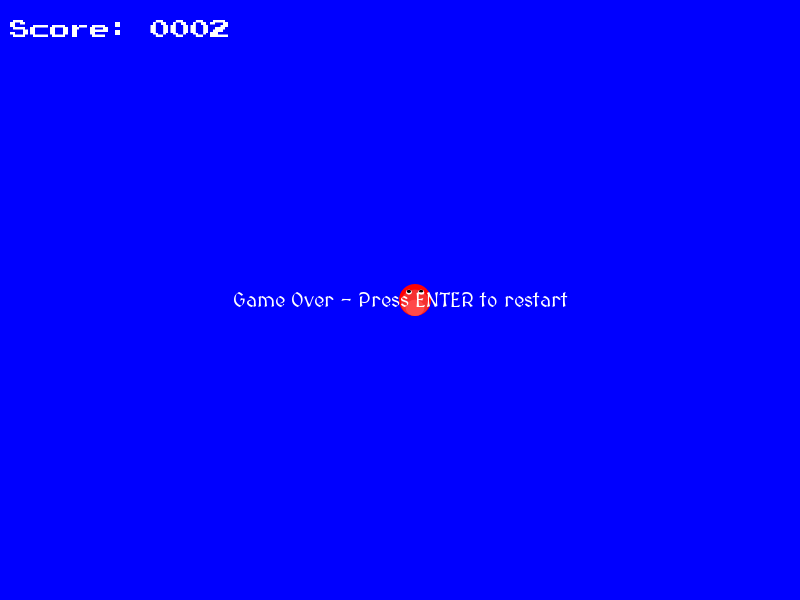
\includegraphics{ss-1-fonts.png}
The default fonts in pygame are good but it adds a nice touch to include a custom font. The process for using fonts is very similar to sound and graphics. You need to register the font location, register a font and then you can refer to it subsequently by the registered name.

\begin{Verbatim}[commandchars=\\\{\},numbers=left,firstnumber=1,stepnumber=1]
\PYG{k+kn}{import} \PYG{n+nn}{serge.visual}
\PYG{n}{serge}\PYG{o}{.}\PYG{n}{visual}\PYG{o}{.}\PYG{n}{Fonts}\PYG{o}{.}\PYG{n}{setPath}\PYG{p}{(}\PYG{l+s}{'}\PYG{l+s}{fonts}\PYG{l+s}{'}\PYG{p}{)}
\PYG{n}{serge}\PYG{o}{.}\PYG{n}{visual}\PYG{o}{.}\PYG{n}{Fonts}\PYG{o}{.}\PYG{n}{registerItem}\PYG{p}{(}\PYG{l+s}{'}\PYG{l+s}{DEFAULT}\PYG{l+s}{'}\PYG{p}{,} \PYG{l+s}{'}\PYG{l+s}{MedievalSharp.ttf}\PYG{l+s}{'}\PYG{p}{)}
\PYG{n}{serge}\PYG{o}{.}\PYG{n}{visual}\PYG{o}{.}\PYG{n}{Fonts}\PYG{o}{.}\PYG{n}{registerItem}\PYG{p}{(}\PYG{l+s}{'}\PYG{l+s}{scores}\PYG{l+s}{'}\PYG{p}{,} \PYG{l+s}{'}\PYG{l+s}{PressStart2P.ttf}\PYG{l+s}{'}\PYG{p}{)}
\end{Verbatim}

You for fonts there is also a special name, \emph{DEFAULT}. If you register a font with this name then this will be the one used by default for all text.

We are using two fonts here, one for the main text and one for the scores. You probably don't need to do this in such a simple game but it allows us to see the difference between using the default font and a named font. All classes involving text take some kind of \emph{font\_name} parameter. If you do not pass anything then the default font is used. Alternatively you pass the name of a registered font and it will use that one.

Note that in the updated game we had to move the score text over a bit as the chosen font is larger than the default.

\begin{Verbatim}[commandchars=\\\{\},numbers=left,firstnumber=1,stepnumber=1]
\PYG{k+kn}{import} \PYG{n+nn}{pygame}

\PYG{k+kn}{import} \PYG{n+nn}{serge.visual}
\PYG{k+kn}{import} \PYG{n+nn}{serge.sound}
\PYG{k+kn}{import} \PYG{n+nn}{serge.engine}
\PYG{k+kn}{import} \PYG{n+nn}{serge.actor}
\PYG{k+kn}{import} \PYG{n+nn}{serge.blocks.visualblocks}
\PYG{k+kn}{import} \PYG{n+nn}{serge.blocks.utils}
\PYG{k+kn}{import} \PYG{n+nn}{serge.blocks.directions}
\PYG{k+kn}{import} \PYG{n+nn}{serge.blocks.behaviours}
\PYG{k+kn}{import} \PYG{n+nn}{serge.blocks.actors}

\PYG{k}{class} \PYG{n+nc}{Snake}\PYG{p}{(}\PYG{n}{serge}\PYG{o}{.}\PYG{n}{actor}\PYG{o}{.}\PYG{n}{CompositeActor}\PYG{p}{)}\PYG{p}{:}
    \PYG{l+s+sd}{"""Represents the snake"""}

    \PYG{k}{def} \PYG{n+nf}{\PYGZus{}\PYGZus{}init\PYGZus{}\PYGZus{}}\PYG{p}{(}\PYG{n+nb+bp}{self}\PYG{p}{)}\PYG{p}{:}
        \PYG{l+s+sd}{"""Initialise the snake"""}
        \PYG{n+nb}{super}\PYG{p}{(}\PYG{n}{Snake}\PYG{p}{,} \PYG{n+nb+bp}{self}\PYG{p}{)}\PYG{o}{.}\PYG{n}{\PYGZus{}\PYGZus{}init\PYGZus{}\PYGZus{}}\PYG{p}{(}\PYG{l+s}{'}\PYG{l+s}{snake}\PYG{l+s}{'}\PYG{p}{,} \PYG{l+s}{'}\PYG{l+s}{snake-head}\PYG{l+s}{'}\PYG{p}{)}
        \PYG{n+nb+bp}{self}\PYG{o}{.}\PYG{n}{visual} \PYG{o}{=} \PYG{n}{serge}\PYG{o}{.}\PYG{n}{blocks}\PYG{o}{.}\PYG{n}{visualblocks}\PYG{o}{.}\PYG{n}{Circle}\PYG{p}{(}\PYG{l+m+mi}{16}\PYG{p}{,} \PYG{p}{(}\PYG{l+m+mi}{0}\PYG{p}{,}\PYG{l+m+mi}{255}\PYG{p}{,}\PYG{l+m+mi}{0}\PYG{p}{)}\PYG{p}{)}
        \PYG{n+nb+bp}{self}\PYG{o}{.}\PYG{n}{setSpriteName}\PYG{p}{(}\PYG{l+s}{'}\PYG{l+s}{head}\PYG{l+s}{'}\PYG{p}{)}
        \PYG{n+nb+bp}{self}\PYG{o}{.}\PYG{n}{setLayerName}\PYG{p}{(}\PYG{l+s}{'}\PYG{l+s}{middle}\PYG{l+s}{'}\PYG{p}{)}
        \PYG{n+nb+bp}{self}\PYG{o}{.}\PYG{n}{current\PYGZus{}direction} \PYG{o}{=} \PYG{n}{serge}\PYG{o}{.}\PYG{n}{blocks}\PYG{o}{.}\PYG{n}{directions}\PYG{o}{.}\PYG{n}{N}
        \PYG{n+nb+bp}{self}\PYG{o}{.}\PYG{n}{is\PYGZus{}dying} \PYG{o}{=} \PYG{n+nb+bp}{False}

    \PYG{k}{def} \PYG{n+nf}{addedToWorld}\PYG{p}{(}\PYG{n+nb+bp}{self}\PYG{p}{,} \PYG{n}{world}\PYG{p}{)}\PYG{p}{:}
        \PYG{l+s+sd}{"""The snake was added to the world"""}
        \PYG{n+nb}{super}\PYG{p}{(}\PYG{n}{Snake}\PYG{p}{,} \PYG{n+nb+bp}{self}\PYG{p}{)}\PYG{o}{.}\PYG{n}{addedToWorld}\PYG{p}{(}\PYG{n}{world}\PYG{p}{)}
        \PYG{c}{\PYGZsh{}}
        \PYG{n+nb+bp}{self}\PYG{o}{.}\PYG{n}{keyboard} \PYG{o}{=} \PYG{n}{serge}\PYG{o}{.}\PYG{n}{engine}\PYG{o}{.}\PYG{n}{CurrentEngine}\PYG{p}{(}\PYG{p}{)}\PYG{o}{.}\PYG{n}{getKeyboard}\PYG{p}{(}\PYG{p}{)}
        \PYG{n+nb+bp}{self}\PYG{o}{.}\PYG{n}{manager} \PYG{o}{=} \PYG{n}{serge}\PYG{o}{.}\PYG{n}{blocks}\PYG{o}{.}\PYG{n}{behaviours}\PYG{o}{.}\PYG{n}{BehaviourManager}\PYG{p}{(}\PYG{l+s}{'}\PYG{l+s}{manager}\PYG{l+s}{'}\PYG{p}{,} \PYG{l+s}{'}\PYG{l+s}{behaviour-manager}\PYG{l+s}{'}\PYG{p}{)}
        \PYG{n}{world}\PYG{o}{.}\PYG{n}{addActor}\PYG{p}{(}\PYG{n+nb+bp}{self}\PYG{o}{.}\PYG{n}{manager}\PYG{p}{)}
        \PYG{c}{\PYGZsh{}}
        \PYG{c}{\PYGZsh{} Text to display when the game is over}
        \PYG{n+nb+bp}{self}\PYG{o}{.}\PYG{n}{restart\PYGZus{}text} \PYG{o}{=} \PYG{n}{serge}\PYG{o}{.}\PYG{n}{blocks}\PYG{o}{.}\PYG{n}{utils}\PYG{o}{.}\PYG{n}{addVisualActorToWorld}\PYG{p}{(}\PYG{n}{world}\PYG{p}{,} \PYG{l+s}{'}\PYG{l+s}{text}\PYG{l+s}{'}\PYG{p}{,} \PYG{l+s}{'}\PYG{l+s}{restart}\PYG{l+s}{'}\PYG{p}{,}
            \PYG{n}{serge}\PYG{o}{.}\PYG{n}{visual}\PYG{o}{.}\PYG{n}{Text}\PYG{p}{(}\PYG{l+s}{'}\PYG{l+s}{Game Over - Press ENTER to restart}\PYG{l+s}{'}\PYG{p}{,} \PYG{p}{(}\PYG{l+m+mi}{255}\PYG{p}{,} \PYG{l+m+mi}{255}\PYG{p}{,} \PYG{l+m+mi}{255}\PYG{p}{)}\PYG{p}{,} \PYG{n}{font\PYGZus{}size}\PYG{o}{=}\PYG{l+m+mi}{20}\PYG{p}{)}\PYG{p}{,}
            \PYG{n}{layer\PYGZus{}name}\PYG{o}{=}\PYG{l+s}{'}\PYG{l+s}{front}\PYG{l+s}{'}\PYG{p}{,}
            \PYG{n}{center\PYGZus{}position}\PYG{o}{=}\PYG{p}{(}\PYG{l+m+mi}{400}\PYG{p}{,} \PYG{l+m+mi}{300}\PYG{p}{)}\PYG{p}{)}
        \PYG{n+nb+bp}{self}\PYG{o}{.}\PYG{n}{restart\PYGZus{}text}\PYG{o}{.}\PYG{n}{visible} \PYG{o}{=} \PYG{n+nb+bp}{False}
        \PYG{c}{\PYGZsh{}}
        \PYG{c}{\PYGZsh{} A background for the game}
        \PYG{n+nb+bp}{self}\PYG{o}{.}\PYG{n}{bg} \PYG{o}{=} \PYG{n}{serge}\PYG{o}{.}\PYG{n}{blocks}\PYG{o}{.}\PYG{n}{utils}\PYG{o}{.}\PYG{n}{addVisualActorToWorld}\PYG{p}{(}\PYG{n}{world}\PYG{p}{,} \PYG{l+s}{'}\PYG{l+s}{bg}\PYG{l+s}{'}\PYG{p}{,} \PYG{l+s}{'}\PYG{l+s}{bg}\PYG{l+s}{'}\PYG{p}{,}
            \PYG{n}{serge}\PYG{o}{.}\PYG{n}{blocks}\PYG{o}{.}\PYG{n}{visualblocks}\PYG{o}{.}\PYG{n}{Rectangle}\PYG{p}{(}\PYG{p}{(}\PYG{l+m+mi}{800}\PYG{p}{,} \PYG{l+m+mi}{600}\PYG{p}{)}\PYG{p}{,} \PYG{p}{(}\PYG{l+m+mi}{0}\PYG{p}{,}\PYG{l+m+mi}{0}\PYG{p}{,}\PYG{l+m+mi}{255}\PYG{p}{)}\PYG{p}{)}\PYG{p}{,}
            \PYG{n}{layer\PYGZus{}name}\PYG{o}{=}\PYG{l+s}{'}\PYG{l+s}{back}\PYG{l+s}{'}\PYG{p}{,}
            \PYG{n}{center\PYGZus{}position}\PYG{o}{=}\PYG{p}{(}\PYG{l+m+mi}{400}\PYG{p}{,} \PYG{l+m+mi}{300}\PYG{p}{)}\PYG{p}{)}
        \PYG{c}{\PYGZsh{}}
        \PYG{c}{\PYGZsh{} Text to show the score}
        \PYG{n+nb+bp}{self}\PYG{o}{.}\PYG{n}{score} \PYG{o}{=} \PYG{n}{serge}\PYG{o}{.}\PYG{n}{blocks}\PYG{o}{.}\PYG{n}{utils}\PYG{o}{.}\PYG{n}{addActorToWorld}\PYG{p}{(}\PYG{n}{world}\PYG{p}{,}
            \PYG{n}{serge}\PYG{o}{.}\PYG{n}{blocks}\PYG{o}{.}\PYG{n}{actors}\PYG{o}{.}\PYG{n}{NumericText}\PYG{p}{(}\PYG{l+s}{'}\PYG{l+s}{text}\PYG{l+s}{'}\PYG{p}{,} \PYG{l+s}{'}\PYG{l+s}{score}\PYG{l+s}{'}\PYG{p}{,} \PYG{l+s}{'}\PYG{l+s}{Score: }\PYG{l+s+si}{\PYGZpc{}04d}\PYG{l+s}{'}\PYG{p}{,}
                \PYG{p}{(}\PYG{l+m+mi}{255}\PYG{p}{,} \PYG{l+m+mi}{255}\PYG{p}{,} \PYG{l+m+mi}{255}\PYG{p}{)}\PYG{p}{,} \PYG{n}{font\PYGZus{}size}\PYG{o}{=}\PYG{l+m+mi}{20}\PYG{p}{,} \PYG{n}{font\PYGZus{}name}\PYG{o}{=}\PYG{l+s}{'}\PYG{l+s}{scores}\PYG{l+s}{'}\PYG{p}{,} \PYG{n}{value}\PYG{o}{=}\PYG{l+m+mi}{0}\PYG{p}{,} \PYG{n}{align}\PYG{o}{=}\PYG{l+s}{'}\PYG{l+s}{left}\PYG{l+s}{'}\PYG{p}{)}\PYG{p}{,}
            \PYG{n}{layer\PYGZus{}name}\PYG{o}{=}\PYG{l+s}{'}\PYG{l+s}{front}\PYG{l+s}{'}\PYG{p}{,}
            \PYG{n}{center\PYGZus{}position}\PYG{o}{=}\PYG{p}{(}\PYG{l+m+mi}{120}\PYG{p}{,} \PYG{l+m+mi}{30}\PYG{p}{)}\PYG{p}{)}

    \PYG{k}{def} \PYG{n+nf}{updateActor}\PYG{p}{(}\PYG{n+nb+bp}{self}\PYG{p}{,} \PYG{n}{interval}\PYG{p}{,} \PYG{n}{world}\PYG{p}{)}\PYG{p}{:}
        \PYG{l+s+sd}{"""Update the snake"""}
        \PYG{n+nb}{super}\PYG{p}{(}\PYG{n}{Snake}\PYG{p}{,} \PYG{n+nb+bp}{self}\PYG{p}{)}\PYG{o}{.}\PYG{n}{updateActor}\PYG{p}{(}\PYG{n}{interval}\PYG{p}{,} \PYG{n}{world}\PYG{p}{)}
        \PYG{c}{\PYGZsh{}}
        \PYG{c}{\PYGZsh{} Quit if requested}
        \PYG{k}{if} \PYG{n+nb+bp}{self}\PYG{o}{.}\PYG{n}{keyboard}\PYG{o}{.}\PYG{n}{isClicked}\PYG{p}{(}\PYG{n}{pygame}\PYG{o}{.}\PYG{n}{K\PYGZus{}ESCAPE}\PYG{p}{)}\PYG{p}{:}
            \PYG{n}{serge}\PYG{o}{.}\PYG{n}{engine}\PYG{o}{.}\PYG{n}{CurrentEngine}\PYG{p}{(}\PYG{p}{)}\PYG{o}{.}\PYG{n}{stop}\PYG{p}{(}\PYG{p}{)}
        \PYG{c}{\PYGZsh{}}
        \PYG{c}{\PYGZsh{} Move the head}
        \PYG{k}{if} \PYG{n+nb+bp}{self}\PYG{o}{.}\PYG{n}{keyboard}\PYG{o}{.}\PYG{n}{isClicked}\PYG{p}{(}\PYG{n}{pygame}\PYG{o}{.}\PYG{n}{K\PYGZus{}LEFT}\PYG{p}{)}\PYG{p}{:}
            \PYG{n}{rotation} \PYG{o}{=} \PYG{o}{+}\PYG{l+m+mi}{90}
        \PYG{k}{elif} \PYG{n+nb+bp}{self}\PYG{o}{.}\PYG{n}{keyboard}\PYG{o}{.}\PYG{n}{isClicked}\PYG{p}{(}\PYG{n}{pygame}\PYG{o}{.}\PYG{n}{K\PYGZus{}RIGHT}\PYG{p}{)}\PYG{p}{:}
            \PYG{n}{rotation} \PYG{o}{=} \PYG{o}{-}\PYG{l+m+mi}{90}
        \PYG{k}{else}\PYG{p}{:}
            \PYG{n}{rotation} \PYG{o}{=} \PYG{l+m+mi}{0}
        \PYG{c}{\PYGZsh{}}
        \PYG{c}{\PYGZsh{} Change direction}
        \PYG{k}{if} \PYG{n}{rotation}\PYG{p}{:}
            \PYG{n}{current\PYGZus{}angle} \PYG{o}{=} \PYG{n}{serge}\PYG{o}{.}\PYG{n}{blocks}\PYG{o}{.}\PYG{n}{directions}\PYG{o}{.}\PYG{n}{getAngleFromCardinal}\PYG{p}{(}\PYG{n+nb+bp}{self}\PYG{o}{.}\PYG{n}{current\PYGZus{}direction}\PYG{p}{)}
            \PYG{n+nb+bp}{self}\PYG{o}{.}\PYG{n}{current\PYGZus{}direction} \PYG{o}{=} \PYG{n}{serge}\PYG{o}{.}\PYG{n}{blocks}\PYG{o}{.}\PYG{n}{directions}\PYG{o}{.}\PYG{n}{getCardinalFromAngle}\PYG{p}{(}\PYG{n}{current\PYGZus{}angle}\PYG{o}{+}\PYG{n}{rotation}\PYG{p}{)}
            \PYG{n+nb+bp}{self}\PYG{o}{.}\PYG{n}{visual}\PYG{o}{.}\PYG{n}{setAngle}\PYG{p}{(}\PYG{n}{current\PYGZus{}angle}\PYG{o}{+}\PYG{n}{rotation}\PYG{p}{)}
        \PYG{c}{\PYGZsh{}}
        \PYG{c}{\PYGZsh{} Move}
        \PYG{k}{if} \PYG{o+ow}{not} \PYG{n+nb+bp}{self}\PYG{o}{.}\PYG{n}{is\PYGZus{}dying}\PYG{p}{:}
            \PYG{n}{offset} \PYG{o}{=} \PYG{l+m+mi}{5}\PYG{o}{*}\PYG{n}{serge}\PYG{o}{.}\PYG{n}{blocks}\PYG{o}{.}\PYG{n}{directions}\PYG{o}{.}\PYG{n}{getVectorFromCardinal}\PYG{p}{(}\PYG{n+nb+bp}{self}\PYG{o}{.}\PYG{n}{current\PYGZus{}direction}\PYG{p}{)}
            \PYG{n+nb+bp}{self}\PYG{o}{.}\PYG{n}{move}\PYG{p}{(}\PYG{o}{*}\PYG{n}{offset}\PYG{p}{)}
            \PYG{c}{\PYGZsh{}}
            \PYG{c}{\PYGZsh{} Add a new segment if needed}
            \PYG{k}{if} \PYG{o+ow}{not} \PYG{n+nb+bp}{self}\PYG{o}{.}\PYG{n}{getChildren}\PYG{p}{(}\PYG{p}{)} \PYG{o+ow}{or} \PYG{n+nb+bp}{self}\PYG{o}{.}\PYG{n}{getDistanceFrom}\PYG{p}{(}\PYG{n+nb+bp}{self}\PYG{o}{.}\PYG{n}{getChildren}\PYG{p}{(}\PYG{p}{)}\PYG{p}{[}\PYG{o}{-}\PYG{l+m+mi}{1}\PYG{p}{]}\PYG{p}{)} \PYG{o}{\textgreater{}} \PYG{l+m+mi}{16}\PYG{p}{:}
                \PYG{n+nb+bp}{self}\PYG{o}{.}\PYG{n}{addSegment}\PYG{p}{(}\PYG{p}{)}
            \PYG{c}{\PYGZsh{}}
            \PYG{c}{\PYGZsh{} Check if we hit the body}
            \PYG{k}{if} \PYG{n+nb+bp}{self}\PYG{o}{.}\PYG{n}{hitBody}\PYG{p}{(}\PYG{p}{)} \PYG{o+ow}{or} \PYG{n+nb+bp}{self}\PYG{o}{.}\PYG{n}{offScreen}\PYG{p}{(}\PYG{p}{)}\PYG{p}{:}
                \PYG{n+nb+bp}{self}\PYG{o}{.}\PYG{n}{initiateDeathAnimation}\PYG{p}{(}\PYG{p}{)}
            \PYG{c}{\PYGZsh{}}
            \PYG{c}{\PYGZsh{} Increase score}
            \PYG{n+nb+bp}{self}\PYG{o}{.}\PYG{n}{score}\PYG{o}{.}\PYG{n}{value} \PYG{o}{+}\PYG{o}{=} \PYG{n}{interval}\PYG{o}{/}\PYG{l+m+mf}{1000.0}
        \PYG{k}{elif} \PYG{n+nb+bp}{self}\PYG{o}{.}\PYG{n}{animation}\PYG{o}{.}\PYG{n}{isComplete}\PYG{p}{(}\PYG{p}{)}\PYG{p}{:}
            \PYG{k}{if} \PYG{n+nb+bp}{self}\PYG{o}{.}\PYG{n}{keyboard}\PYG{o}{.}\PYG{n}{isClicked}\PYG{p}{(}\PYG{n}{pygame}\PYG{o}{.}\PYG{n}{K\PYGZus{}KP\PYGZus{}ENTER}\PYG{p}{)} \PYG{o+ow}{or} \PYG{n+nb+bp}{self}\PYG{o}{.}\PYG{n}{keyboard}\PYG{o}{.}\PYG{n}{isClicked}\PYG{p}{(}\PYG{n}{pygame}\PYG{o}{.}\PYG{n}{K\PYGZus{}RETURN}\PYG{p}{)}\PYG{p}{:}
                \PYG{n+nb+bp}{self}\PYG{o}{.}\PYG{n}{restartGame}\PYG{p}{(}\PYG{p}{)}

    \PYG{k}{def} \PYG{n+nf}{addSegment}\PYG{p}{(}\PYG{n+nb+bp}{self}\PYG{p}{)}\PYG{p}{:}
        \PYG{l+s+sd}{"""Add a new body segment"""}
        \PYG{n}{segment} \PYG{o}{=} \PYG{n}{serge}\PYG{o}{.}\PYG{n}{actor}\PYG{o}{.}\PYG{n}{Actor}\PYG{p}{(}\PYG{l+s}{'}\PYG{l+s}{segment}\PYG{l+s}{'}\PYG{p}{)}
        \PYG{n}{segment}\PYG{o}{.}\PYG{n}{visual} \PYG{o}{=} \PYG{n}{serge}\PYG{o}{.}\PYG{n}{blocks}\PYG{o}{.}\PYG{n}{visualblocks}\PYG{o}{.}\PYG{n}{Circle}\PYG{p}{(}\PYG{l+m+mi}{16}\PYG{p}{,} \PYG{p}{(}\PYG{l+m+mi}{0}\PYG{p}{,}\PYG{l+m+mi}{200}\PYG{p}{,}\PYG{l+m+mi}{0}\PYG{p}{)}\PYG{p}{)}
        \PYG{n}{segment}\PYG{o}{.}\PYG{n}{setSpriteName}\PYG{p}{(}\PYG{l+s}{'}\PYG{l+s}{tail}\PYG{l+s}{'}\PYG{p}{)}
        \PYG{n}{segment}\PYG{o}{.}\PYG{n}{setLayerName}\PYG{p}{(}\PYG{l+s}{'}\PYG{l+s}{middle}\PYG{l+s}{'}\PYG{p}{)}
        \PYG{n}{segment}\PYG{o}{.}\PYG{n}{moveTo}\PYG{p}{(}\PYG{n+nb+bp}{self}\PYG{o}{.}\PYG{n}{x}\PYG{p}{,} \PYG{n+nb+bp}{self}\PYG{o}{.}\PYG{n}{y}\PYG{p}{)}
        \PYG{n+nb+bp}{self}\PYG{o}{.}\PYG{n}{addChild}\PYG{p}{(}\PYG{n}{segment}\PYG{p}{)}
        \PYG{n}{serge}\PYG{o}{.}\PYG{n}{sound}\PYG{o}{.}\PYG{n}{Sounds}\PYG{o}{.}\PYG{n}{play}\PYG{p}{(}\PYG{l+s}{'}\PYG{l+s}{new-body}\PYG{l+s}{'}\PYG{p}{)}

    \PYG{k}{def} \PYG{n+nf}{hitBody}\PYG{p}{(}\PYG{n+nb+bp}{self}\PYG{p}{)}\PYG{p}{:}
        \PYG{l+s+sd}{"""Return True if the head has hit the body}

\PYG{l+s+sd}{        Look to see if we overlap with any body segment except the last}
\PYG{l+s+sd}{        (we are allowed to overlap the last since we just put it down)}

\PYG{l+s+sd}{        """}
        \PYG{k}{for} \PYG{n}{segment} \PYG{o+ow}{in} \PYG{n+nb+bp}{self}\PYG{o}{.}\PYG{n}{getChildren}\PYG{p}{(}\PYG{p}{)}\PYG{p}{[}\PYG{p}{:}\PYG{o}{-}\PYG{l+m+mi}{1}\PYG{p}{]}\PYG{p}{:}
            \PYG{k}{if} \PYG{n+nb+bp}{self}\PYG{o}{.}\PYG{n}{getDistanceFrom}\PYG{p}{(}\PYG{n}{segment}\PYG{p}{)} \PYG{o}{\textless{}} \PYG{l+m+mi}{16}\PYG{p}{:}
                \PYG{k}{return} \PYG{n+nb+bp}{True}
        \PYG{k}{return} \PYG{n+nb+bp}{False}

    \PYG{k}{def} \PYG{n+nf}{offScreen}\PYG{p}{(}\PYG{n+nb+bp}{self}\PYG{p}{)}\PYG{p}{:}
        \PYG{l+s+sd}{"""Return True if we are off the screen"""}
        \PYG{k}{return} \PYG{n+nb+bp}{self}\PYG{o}{.}\PYG{n}{x} \PYG{o}{\textless{}} \PYG{l+m+mi}{0} \PYG{o+ow}{or} \PYG{n+nb+bp}{self}\PYG{o}{.}\PYG{n}{x} \PYG{o}{\textgreater{}} \PYG{l+m+mi}{800} \PYG{o+ow}{or} \PYG{n+nb+bp}{self}\PYG{o}{.}\PYG{n}{y} \PYG{o}{\textless{}} \PYG{l+m+mi}{0} \PYG{o+ow}{or} \PYG{n+nb+bp}{self}\PYG{o}{.}\PYG{n}{y} \PYG{o}{\textgreater{}} \PYG{l+m+mi}{600}

    \PYG{k}{def} \PYG{n+nf}{initiateDeathAnimation}\PYG{p}{(}\PYG{n+nb+bp}{self}\PYG{p}{)}\PYG{p}{:}
        \PYG{l+s+sd}{"""Begin showing the death of the snake"""}
        \PYG{n+nb+bp}{self}\PYG{o}{.}\PYG{n}{log}\PYG{o}{.}\PYG{n}{info}\PYG{p}{(}\PYG{l+s}{'}\PYG{l+s}{Snake died!}\PYG{l+s}{'}\PYG{p}{)}
        \PYG{n+nb+bp}{self}\PYG{o}{.}\PYG{n}{animation} \PYG{o}{=} \PYG{n+nb+bp}{self}\PYG{o}{.}\PYG{n}{manager}\PYG{o}{.}\PYG{n}{assignBehaviour}\PYG{p}{(}\PYG{n+nb+bp}{self}\PYG{p}{,}
            \PYG{n}{serge}\PYG{o}{.}\PYG{n}{blocks}\PYG{o}{.}\PYG{n}{behaviours}\PYG{o}{.}\PYG{n}{TimedCallback}\PYG{p}{(}\PYG{l+m+mi}{1000}\PYG{o}{/}\PYG{n+nb}{len}\PYG{p}{(}\PYG{n+nb+bp}{self}\PYG{o}{.}\PYG{n}{getChildren}\PYG{p}{(}\PYG{p}{)}\PYG{p}{)}\PYG{p}{,} \PYG{n+nb+bp}{self}\PYG{o}{.}\PYG{n}{removeTail}\PYG{p}{)}\PYG{p}{,} \PYG{l+s}{'}\PYG{l+s}{death-animation}\PYG{l+s}{'}\PYG{p}{)}
        \PYG{n+nb+bp}{self}\PYG{o}{.}\PYG{n}{is\PYGZus{}dying} \PYG{o}{=} \PYG{n+nb+bp}{True}
        \PYG{k}{for} \PYG{n}{segment} \PYG{o+ow}{in} \PYG{n+nb+bp}{self}\PYG{o}{.}\PYG{n}{getChildren}\PYG{p}{(}\PYG{p}{)}\PYG{p}{:}
            \PYG{n}{segment}\PYG{o}{.}\PYG{n}{setSpriteName}\PYG{p}{(}\PYG{l+s}{'}\PYG{l+s}{red-tail}\PYG{l+s}{'}\PYG{p}{)}
        \PYG{n+nb+bp}{self}\PYG{o}{.}\PYG{n}{setSpriteName}\PYG{p}{(}\PYG{l+s}{'}\PYG{l+s}{red-head}\PYG{l+s}{'}\PYG{p}{)}
        \PYG{n}{serge}\PYG{o}{.}\PYG{n}{sound}\PYG{o}{.}\PYG{n}{Sounds}\PYG{o}{.}\PYG{n}{play}\PYG{p}{(}\PYG{l+s}{'}\PYG{l+s}{snake-death}\PYG{l+s}{'}\PYG{p}{)}

    \PYG{k}{def} \PYG{n+nf}{removeTail}\PYG{p}{(}\PYG{n+nb+bp}{self}\PYG{p}{,} \PYG{n}{world}\PYG{p}{,} \PYG{n}{actor}\PYG{p}{,} \PYG{n}{interval}\PYG{p}{)}\PYG{p}{:}
        \PYG{l+s+sd}{"""Remove part of the tail"""}
        \PYG{n+nb+bp}{self}\PYG{o}{.}\PYG{n}{log}\PYG{o}{.}\PYG{n}{debug}\PYG{p}{(}\PYG{l+s}{'}\PYG{l+s}{Removing part of the tail}\PYG{l+s}{'}\PYG{p}{)}
        \PYG{k}{if} \PYG{n+nb+bp}{self}\PYG{o}{.}\PYG{n}{getChildren}\PYG{p}{(}\PYG{p}{)}\PYG{p}{:}
            \PYG{n+nb+bp}{self}\PYG{o}{.}\PYG{n}{removeChild}\PYG{p}{(}\PYG{n+nb+bp}{self}\PYG{o}{.}\PYG{n}{getChildren}\PYG{p}{(}\PYG{p}{)}\PYG{p}{[}\PYG{l+m+mi}{0}\PYG{p}{]}\PYG{p}{)}
        \PYG{k}{else}\PYG{p}{:}
            \PYG{n+nb+bp}{self}\PYG{o}{.}\PYG{n}{animation}\PYG{o}{.}\PYG{n}{markComplete}\PYG{p}{(}\PYG{p}{)}
            \PYG{n+nb+bp}{self}\PYG{o}{.}\PYG{n}{restart\PYGZus{}text}\PYG{o}{.}\PYG{n}{visible} \PYG{o}{=} \PYG{n+nb+bp}{True}
            \PYG{n}{serge}\PYG{o}{.}\PYG{n}{sound}\PYG{o}{.}\PYG{n}{Sounds}\PYG{o}{.}\PYG{n}{getItem}\PYG{p}{(}\PYG{l+s}{'}\PYG{l+s}{snake-death}\PYG{l+s}{'}\PYG{p}{)}\PYG{o}{.}\PYG{n}{fadeout}\PYG{p}{(}\PYG{l+m+mi}{500}\PYG{p}{)}

    \PYG{k}{def} \PYG{n+nf}{restartGame}\PYG{p}{(}\PYG{n+nb+bp}{self}\PYG{p}{)}\PYG{p}{:}
        \PYG{l+s+sd}{"""Restart the game"""}
        \PYG{n+nb+bp}{self}\PYG{o}{.}\PYG{n}{is\PYGZus{}dying} \PYG{o}{=} \PYG{n+nb+bp}{False}
        \PYG{n+nb+bp}{self}\PYG{o}{.}\PYG{n}{restart\PYGZus{}text}\PYG{o}{.}\PYG{n}{visible} \PYG{o}{=} \PYG{n+nb+bp}{False}
        \PYG{n+nb+bp}{self}\PYG{o}{.}\PYG{n}{setSpriteName}\PYG{p}{(}\PYG{l+s}{'}\PYG{l+s}{head}\PYG{l+s}{'}\PYG{p}{)}
        \PYG{n+nb+bp}{self}\PYG{o}{.}\PYG{n}{current\PYGZus{}direction} \PYG{o}{=} \PYG{n}{serge}\PYG{o}{.}\PYG{n}{blocks}\PYG{o}{.}\PYG{n}{directions}\PYG{o}{.}\PYG{n}{N}
        \PYG{n+nb+bp}{self}\PYG{o}{.}\PYG{n}{score}\PYG{o}{.}\PYG{n}{value} \PYG{o}{=} \PYG{l+m+mi}{0}
        \PYG{n+nb+bp}{self}\PYG{o}{.}\PYG{n}{moveTo}\PYG{p}{(}\PYG{l+m+mi}{400}\PYG{p}{,} \PYG{l+m+mi}{300}\PYG{p}{)}

\PYG{c}{\PYGZsh{} Create the engine}
\PYG{n}{engine} \PYG{o}{=} \PYG{n}{serge}\PYG{o}{.}\PYG{n}{blocks}\PYG{o}{.}\PYG{n}{utils}\PYG{o}{.}\PYG{n}{getSimpleSetup}\PYG{p}{(}\PYG{l+m+mi}{800}\PYG{p}{,} \PYG{l+m+mi}{600}\PYG{p}{)}
\PYG{n}{world} \PYG{o}{=} \PYG{n}{engine}\PYG{o}{.}\PYG{n}{getWorld}\PYG{p}{(}\PYG{l+s}{'}\PYG{l+s}{lab}\PYG{l+s}{'}\PYG{p}{)}

\PYG{c}{\PYGZsh{} Register sprites}
\PYG{n}{serge}\PYG{o}{.}\PYG{n}{visual}\PYG{o}{.}\PYG{n}{Sprites}\PYG{o}{.}\PYG{n}{setPath}\PYG{p}{(}\PYG{l+s}{'}\PYG{l+s}{graphics}\PYG{l+s}{'}\PYG{p}{)}
\PYG{n}{serge}\PYG{o}{.}\PYG{n}{visual}\PYG{o}{.}\PYG{n}{Sprites}\PYG{o}{.}\PYG{n}{registerItem}\PYG{p}{(}\PYG{l+s}{'}\PYG{l+s}{head}\PYG{l+s}{'}\PYG{p}{,} \PYG{l+s}{'}\PYG{l+s}{head.png}\PYG{l+s}{'}\PYG{p}{)}
\PYG{n}{serge}\PYG{o}{.}\PYG{n}{visual}\PYG{o}{.}\PYG{n}{Sprites}\PYG{o}{.}\PYG{n}{registerItem}\PYG{p}{(}\PYG{l+s}{'}\PYG{l+s}{tail}\PYG{l+s}{'}\PYG{p}{,} \PYG{l+s}{'}\PYG{l+s}{tail.png}\PYG{l+s}{'}\PYG{p}{)}
\PYG{n}{serge}\PYG{o}{.}\PYG{n}{visual}\PYG{o}{.}\PYG{n}{Sprites}\PYG{o}{.}\PYG{n}{registerItem}\PYG{p}{(}\PYG{l+s}{'}\PYG{l+s}{red-head}\PYG{l+s}{'}\PYG{p}{,} \PYG{l+s}{'}\PYG{l+s}{red-head.png}\PYG{l+s}{'}\PYG{p}{)}
\PYG{n}{serge}\PYG{o}{.}\PYG{n}{visual}\PYG{o}{.}\PYG{n}{Sprites}\PYG{o}{.}\PYG{n}{registerItem}\PYG{p}{(}\PYG{l+s}{'}\PYG{l+s}{red-tail}\PYG{l+s}{'}\PYG{p}{,} \PYG{l+s}{'}\PYG{l+s}{red-tail.png}\PYG{l+s}{'}\PYG{p}{)}

\PYG{c}{\PYGZsh{} Register sounds}
\PYG{n}{serge}\PYG{o}{.}\PYG{n}{sound}\PYG{o}{.}\PYG{n}{Sounds}\PYG{o}{.}\PYG{n}{setPath}\PYG{p}{(}\PYG{l+s}{'}\PYG{l+s}{sounds}\PYG{l+s}{'}\PYG{p}{)}
\PYG{n}{serge}\PYG{o}{.}\PYG{n}{sound}\PYG{o}{.}\PYG{n}{Sounds}\PYG{o}{.}\PYG{n}{registerItem}\PYG{p}{(}\PYG{l+s}{'}\PYG{l+s}{new-body}\PYG{l+s}{'}\PYG{p}{,} \PYG{l+s}{'}\PYG{l+s}{bloop.wav}\PYG{l+s}{'}\PYG{p}{)}
\PYG{n}{serge}\PYG{o}{.}\PYG{n}{sound}\PYG{o}{.}\PYG{n}{Sounds}\PYG{o}{.}\PYG{n}{registerItem}\PYG{p}{(}\PYG{l+s}{'}\PYG{l+s}{snake-death}\PYG{l+s}{'}\PYG{p}{,} \PYG{l+s}{'}\PYG{l+s}{death.wav}\PYG{l+s}{'}\PYG{p}{)}

\PYG{c}{\PYGZsh{} Register fonts}
\PYG{n}{serge}\PYG{o}{.}\PYG{n}{visual}\PYG{o}{.}\PYG{n}{Fonts}\PYG{o}{.}\PYG{n}{setPath}\PYG{p}{(}\PYG{l+s}{'}\PYG{l+s}{fonts}\PYG{l+s}{'}\PYG{p}{)}
\PYG{n}{serge}\PYG{o}{.}\PYG{n}{visual}\PYG{o}{.}\PYG{n}{Fonts}\PYG{o}{.}\PYG{n}{registerItem}\PYG{p}{(}\PYG{l+s}{'}\PYG{l+s}{DEFAULT}\PYG{l+s}{'}\PYG{p}{,} \PYG{l+s}{'}\PYG{l+s}{MedievalSharp.ttf}\PYG{l+s}{'}\PYG{p}{)}
\PYG{n}{serge}\PYG{o}{.}\PYG{n}{visual}\PYG{o}{.}\PYG{n}{Fonts}\PYG{o}{.}\PYG{n}{registerItem}\PYG{p}{(}\PYG{l+s}{'}\PYG{l+s}{scores}\PYG{l+s}{'}\PYG{p}{,} \PYG{l+s}{'}\PYG{l+s}{PressStart2P.ttf}\PYG{l+s}{'}\PYG{p}{)}

\PYG{c}{\PYGZsh{} Create the snake}
\PYG{n}{snake} \PYG{o}{=} \PYG{n}{Snake}\PYG{p}{(}\PYG{p}{)}
\PYG{n}{world}\PYG{o}{.}\PYG{n}{addActor}\PYG{p}{(}\PYG{n}{snake}\PYG{p}{)}
\PYG{n}{snake}\PYG{o}{.}\PYG{n}{moveTo}\PYG{p}{(}\PYG{l+m+mi}{400}\PYG{p}{,} \PYG{l+m+mi}{300}\PYG{p}{)}

\PYG{c}{\PYGZsh{} Run the game}
\PYG{n}{engine}\PYG{o}{.}\PYG{n}{run}\PYG{p}{(}\PYG{l+m+mi}{60}\PYG{p}{)}
\end{Verbatim}


\subsection{Additional Gameplay elements}
\label{tutorial-2:additional-gameplay-elements}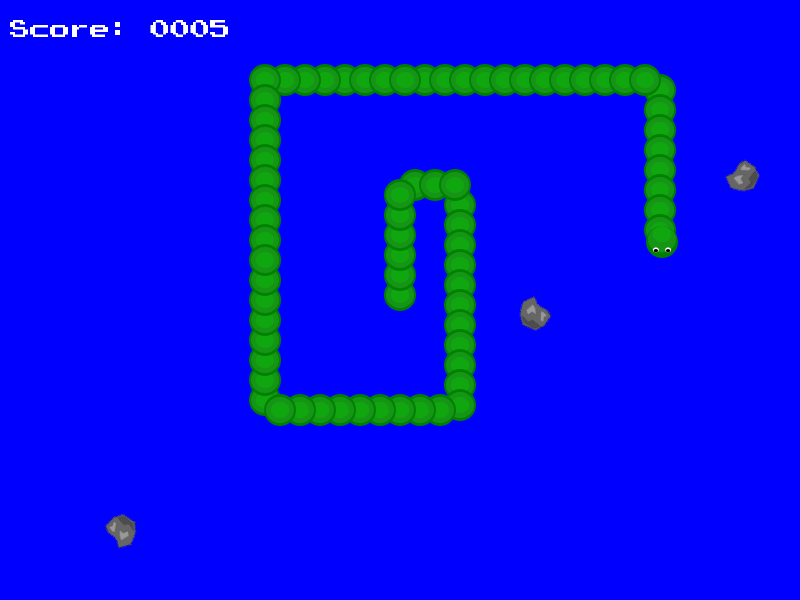
\includegraphics{ss-1-rocks.png}
Before exploring more of the game engine we need to add some more gameplay elements.

Let's add a number of rocks to the screen. If the snake hits a rock then it is
going to die. But later we will allow the player to click on the rocks to blow them
up.

First we need to add a rock graphic and then add some code to add it to the screen. We register
the rock graphic as before, with:

\begin{Verbatim}[commandchars=\\\{\},numbers=left,firstnumber=1,stepnumber=1]
\PYG{n}{serge}\PYG{o}{.}\PYG{n}{visual}\PYG{o}{.}\PYG{n}{Sprites}\PYG{o}{.}\PYG{n}{regsiterItem}\PYG{p}{(}\PYG{l+s}{'}\PYG{l+s}{rock}\PYG{l+s}{'}\PYG{p}{,} \PYG{l+s}{'}\PYG{l+s}{rock.png}\PYG{l+s}{'}\PYG{p}{)}
\end{Verbatim}

Then we will randomly add a rock to the screen every so often in the snakes \emph{updateActor} method. We also
need to check if the snake has hit a rock. We do this in the same method.

When we add a rock we use the line:

\begin{Verbatim}[commandchars=\\\{\},numbers=left,firstnumber=1,stepnumber=1]
\PYG{n}{rock} \PYG{o}{=} \PYG{n}{serge}\PYG{o}{.}\PYG{n}{actor}\PYG{o}{.}\PYG{n}{Actor}\PYG{p}{(}\PYG{l+s}{'}\PYG{l+s}{rock}\PYG{l+s}{'}\PYG{p}{)}
\end{Verbatim}

The text \emph{`rock'} here is the actor's \emph{tag}. Tags are very useful and can be used to locate groups of actors in the world. In this case we are going to use it to later find out all the rocks that we have added without having to manually keep track.

Every actor has a tag and optionally can have a name. You can also find actors by names but names are assumed (but not forced) to be unique.

\begin{Verbatim}[commandchars=\\\{\},numbers=left,firstnumber=1,stepnumber=1]
\PYG{n}{rock} \PYG{o}{=} \PYG{n}{serge}\PYG{o}{.}\PYG{n}{actor}\PYG{o}{.}\PYG{n}{Actor}\PYG{p}{(}\PYG{l+s}{'}\PYG{l+s}{rock}\PYG{l+s}{'}\PYG{p}{,} \PYG{l+s}{'}\PYG{l+s}{rock-63}\PYG{l+s}{'}\PYG{p}{)}
\end{Verbatim}

The new code is as follows.

\begin{Verbatim}[commandchars=\\\{\},numbers=left,firstnumber=1,stepnumber=1]
\PYG{k+kn}{import} \PYG{n+nn}{random}
\PYG{k+kn}{import} \PYG{n+nn}{pygame}

\PYG{k+kn}{import} \PYG{n+nn}{serge.visual}
\PYG{k+kn}{import} \PYG{n+nn}{serge.sound}
\PYG{k+kn}{import} \PYG{n+nn}{serge.engine}
\PYG{k+kn}{import} \PYG{n+nn}{serge.actor}
\PYG{k+kn}{import} \PYG{n+nn}{serge.blocks.visualblocks}
\PYG{k+kn}{import} \PYG{n+nn}{serge.blocks.utils}
\PYG{k+kn}{import} \PYG{n+nn}{serge.blocks.directions}
\PYG{k+kn}{import} \PYG{n+nn}{serge.blocks.behaviours}
\PYG{k+kn}{import} \PYG{n+nn}{serge.blocks.actors}

\PYG{k}{class} \PYG{n+nc}{Snake}\PYG{p}{(}\PYG{n}{serge}\PYG{o}{.}\PYG{n}{actor}\PYG{o}{.}\PYG{n}{CompositeActor}\PYG{p}{)}\PYG{p}{:}
    \PYG{l+s+sd}{"""Represents the snake"""}

    \PYG{k}{def} \PYG{n+nf}{\PYGZus{}\PYGZus{}init\PYGZus{}\PYGZus{}}\PYG{p}{(}\PYG{n+nb+bp}{self}\PYG{p}{)}\PYG{p}{:}
        \PYG{l+s+sd}{"""Initialise the snake"""}
        \PYG{n+nb}{super}\PYG{p}{(}\PYG{n}{Snake}\PYG{p}{,} \PYG{n+nb+bp}{self}\PYG{p}{)}\PYG{o}{.}\PYG{n}{\PYGZus{}\PYGZus{}init\PYGZus{}\PYGZus{}}\PYG{p}{(}\PYG{l+s}{'}\PYG{l+s}{snake}\PYG{l+s}{'}\PYG{p}{,} \PYG{l+s}{'}\PYG{l+s}{snake-head}\PYG{l+s}{'}\PYG{p}{)}
        \PYG{n+nb+bp}{self}\PYG{o}{.}\PYG{n}{visual} \PYG{o}{=} \PYG{n}{serge}\PYG{o}{.}\PYG{n}{blocks}\PYG{o}{.}\PYG{n}{visualblocks}\PYG{o}{.}\PYG{n}{Circle}\PYG{p}{(}\PYG{l+m+mi}{16}\PYG{p}{,} \PYG{p}{(}\PYG{l+m+mi}{0}\PYG{p}{,}\PYG{l+m+mi}{255}\PYG{p}{,}\PYG{l+m+mi}{0}\PYG{p}{)}\PYG{p}{)}
        \PYG{n+nb+bp}{self}\PYG{o}{.}\PYG{n}{setSpriteName}\PYG{p}{(}\PYG{l+s}{'}\PYG{l+s}{head}\PYG{l+s}{'}\PYG{p}{)}
        \PYG{n+nb+bp}{self}\PYG{o}{.}\PYG{n}{setLayerName}\PYG{p}{(}\PYG{l+s}{'}\PYG{l+s}{middle}\PYG{l+s}{'}\PYG{p}{)}
        \PYG{n+nb+bp}{self}\PYG{o}{.}\PYG{n}{current\PYGZus{}direction} \PYG{o}{=} \PYG{n}{serge}\PYG{o}{.}\PYG{n}{blocks}\PYG{o}{.}\PYG{n}{directions}\PYG{o}{.}\PYG{n}{N}
        \PYG{n+nb+bp}{self}\PYG{o}{.}\PYG{n}{is\PYGZus{}dying} \PYG{o}{=} \PYG{n+nb+bp}{False}

    \PYG{k}{def} \PYG{n+nf}{addedToWorld}\PYG{p}{(}\PYG{n+nb+bp}{self}\PYG{p}{,} \PYG{n}{world}\PYG{p}{)}\PYG{p}{:}
        \PYG{l+s+sd}{"""The snake was added to the world"""}
        \PYG{n+nb}{super}\PYG{p}{(}\PYG{n}{Snake}\PYG{p}{,} \PYG{n+nb+bp}{self}\PYG{p}{)}\PYG{o}{.}\PYG{n}{addedToWorld}\PYG{p}{(}\PYG{n}{world}\PYG{p}{)}
        \PYG{c}{\PYGZsh{}}
        \PYG{n+nb+bp}{self}\PYG{o}{.}\PYG{n}{keyboard} \PYG{o}{=} \PYG{n}{serge}\PYG{o}{.}\PYG{n}{engine}\PYG{o}{.}\PYG{n}{CurrentEngine}\PYG{p}{(}\PYG{p}{)}\PYG{o}{.}\PYG{n}{getKeyboard}\PYG{p}{(}\PYG{p}{)}
        \PYG{n+nb+bp}{self}\PYG{o}{.}\PYG{n}{manager} \PYG{o}{=} \PYG{n}{serge}\PYG{o}{.}\PYG{n}{blocks}\PYG{o}{.}\PYG{n}{behaviours}\PYG{o}{.}\PYG{n}{BehaviourManager}\PYG{p}{(}\PYG{l+s}{'}\PYG{l+s}{manager}\PYG{l+s}{'}\PYG{p}{,} \PYG{l+s}{'}\PYG{l+s}{behaviour-manager}\PYG{l+s}{'}\PYG{p}{)}
        \PYG{n+nb+bp}{self}\PYG{o}{.}\PYG{n}{world} \PYG{o}{=} \PYG{n}{world}
        \PYG{n}{world}\PYG{o}{.}\PYG{n}{addActor}\PYG{p}{(}\PYG{n+nb+bp}{self}\PYG{o}{.}\PYG{n}{manager}\PYG{p}{)}
        \PYG{c}{\PYGZsh{}}
        \PYG{c}{\PYGZsh{} Text to display when the game is over}
        \PYG{n+nb+bp}{self}\PYG{o}{.}\PYG{n}{restart\PYGZus{}text} \PYG{o}{=} \PYG{n}{serge}\PYG{o}{.}\PYG{n}{blocks}\PYG{o}{.}\PYG{n}{utils}\PYG{o}{.}\PYG{n}{addVisualActorToWorld}\PYG{p}{(}\PYG{n}{world}\PYG{p}{,} \PYG{l+s}{'}\PYG{l+s}{text}\PYG{l+s}{'}\PYG{p}{,} \PYG{l+s}{'}\PYG{l+s}{restart}\PYG{l+s}{'}\PYG{p}{,}
            \PYG{n}{serge}\PYG{o}{.}\PYG{n}{visual}\PYG{o}{.}\PYG{n}{Text}\PYG{p}{(}\PYG{l+s}{'}\PYG{l+s}{Game Over - Press ENTER to restart}\PYG{l+s}{'}\PYG{p}{,} \PYG{p}{(}\PYG{l+m+mi}{255}\PYG{p}{,} \PYG{l+m+mi}{255}\PYG{p}{,} \PYG{l+m+mi}{255}\PYG{p}{)}\PYG{p}{,} \PYG{n}{font\PYGZus{}size}\PYG{o}{=}\PYG{l+m+mi}{20}\PYG{p}{)}\PYG{p}{,}
            \PYG{n}{layer\PYGZus{}name}\PYG{o}{=}\PYG{l+s}{'}\PYG{l+s}{front}\PYG{l+s}{'}\PYG{p}{,}
            \PYG{n}{center\PYGZus{}position}\PYG{o}{=}\PYG{p}{(}\PYG{l+m+mi}{400}\PYG{p}{,} \PYG{l+m+mi}{300}\PYG{p}{)}\PYG{p}{)}
        \PYG{n+nb+bp}{self}\PYG{o}{.}\PYG{n}{restart\PYGZus{}text}\PYG{o}{.}\PYG{n}{visible} \PYG{o}{=} \PYG{n+nb+bp}{False}
        \PYG{c}{\PYGZsh{}}
        \PYG{c}{\PYGZsh{} A background for the game}
        \PYG{n+nb+bp}{self}\PYG{o}{.}\PYG{n}{bg} \PYG{o}{=} \PYG{n}{serge}\PYG{o}{.}\PYG{n}{blocks}\PYG{o}{.}\PYG{n}{utils}\PYG{o}{.}\PYG{n}{addVisualActorToWorld}\PYG{p}{(}\PYG{n}{world}\PYG{p}{,} \PYG{l+s}{'}\PYG{l+s}{bg}\PYG{l+s}{'}\PYG{p}{,} \PYG{l+s}{'}\PYG{l+s}{bg}\PYG{l+s}{'}\PYG{p}{,}
            \PYG{n}{serge}\PYG{o}{.}\PYG{n}{blocks}\PYG{o}{.}\PYG{n}{visualblocks}\PYG{o}{.}\PYG{n}{Rectangle}\PYG{p}{(}\PYG{p}{(}\PYG{l+m+mi}{800}\PYG{p}{,} \PYG{l+m+mi}{600}\PYG{p}{)}\PYG{p}{,} \PYG{p}{(}\PYG{l+m+mi}{0}\PYG{p}{,}\PYG{l+m+mi}{0}\PYG{p}{,}\PYG{l+m+mi}{255}\PYG{p}{)}\PYG{p}{)}\PYG{p}{,}
            \PYG{n}{layer\PYGZus{}name}\PYG{o}{=}\PYG{l+s}{'}\PYG{l+s}{back}\PYG{l+s}{'}\PYG{p}{,}
            \PYG{n}{center\PYGZus{}position}\PYG{o}{=}\PYG{p}{(}\PYG{l+m+mi}{400}\PYG{p}{,} \PYG{l+m+mi}{300}\PYG{p}{)}\PYG{p}{)}
        \PYG{c}{\PYGZsh{}}
        \PYG{c}{\PYGZsh{} Text to show the score}
        \PYG{n+nb+bp}{self}\PYG{o}{.}\PYG{n}{score} \PYG{o}{=} \PYG{n}{serge}\PYG{o}{.}\PYG{n}{blocks}\PYG{o}{.}\PYG{n}{utils}\PYG{o}{.}\PYG{n}{addActorToWorld}\PYG{p}{(}\PYG{n}{world}\PYG{p}{,}
            \PYG{n}{serge}\PYG{o}{.}\PYG{n}{blocks}\PYG{o}{.}\PYG{n}{actors}\PYG{o}{.}\PYG{n}{NumericText}\PYG{p}{(}\PYG{l+s}{'}\PYG{l+s}{text}\PYG{l+s}{'}\PYG{p}{,} \PYG{l+s}{'}\PYG{l+s}{score}\PYG{l+s}{'}\PYG{p}{,} \PYG{l+s}{'}\PYG{l+s}{Score: }\PYG{l+s+si}{\PYGZpc{}04d}\PYG{l+s}{'}\PYG{p}{,}
                \PYG{p}{(}\PYG{l+m+mi}{255}\PYG{p}{,} \PYG{l+m+mi}{255}\PYG{p}{,} \PYG{l+m+mi}{255}\PYG{p}{)}\PYG{p}{,} \PYG{n}{font\PYGZus{}size}\PYG{o}{=}\PYG{l+m+mi}{20}\PYG{p}{,} \PYG{n}{font\PYGZus{}name}\PYG{o}{=}\PYG{l+s}{'}\PYG{l+s}{scores}\PYG{l+s}{'}\PYG{p}{,} \PYG{n}{value}\PYG{o}{=}\PYG{l+m+mi}{0}\PYG{p}{,} \PYG{n}{align}\PYG{o}{=}\PYG{l+s}{'}\PYG{l+s}{left}\PYG{l+s}{'}\PYG{p}{)}\PYG{p}{,}
            \PYG{n}{layer\PYGZus{}name}\PYG{o}{=}\PYG{l+s}{'}\PYG{l+s}{front}\PYG{l+s}{'}\PYG{p}{,}
            \PYG{n}{center\PYGZus{}position}\PYG{o}{=}\PYG{p}{(}\PYG{l+m+mi}{120}\PYG{p}{,} \PYG{l+m+mi}{30}\PYG{p}{)}\PYG{p}{)}

    \PYG{k}{def} \PYG{n+nf}{updateActor}\PYG{p}{(}\PYG{n+nb+bp}{self}\PYG{p}{,} \PYG{n}{interval}\PYG{p}{,} \PYG{n}{world}\PYG{p}{)}\PYG{p}{:}
        \PYG{l+s+sd}{"""Update the snake"""}
        \PYG{n+nb}{super}\PYG{p}{(}\PYG{n}{Snake}\PYG{p}{,} \PYG{n+nb+bp}{self}\PYG{p}{)}\PYG{o}{.}\PYG{n}{updateActor}\PYG{p}{(}\PYG{n}{interval}\PYG{p}{,} \PYG{n}{world}\PYG{p}{)}
        \PYG{c}{\PYGZsh{}}
        \PYG{c}{\PYGZsh{} Quit if requested}
        \PYG{k}{if} \PYG{n+nb+bp}{self}\PYG{o}{.}\PYG{n}{keyboard}\PYG{o}{.}\PYG{n}{isClicked}\PYG{p}{(}\PYG{n}{pygame}\PYG{o}{.}\PYG{n}{K\PYGZus{}ESCAPE}\PYG{p}{)}\PYG{p}{:}
            \PYG{n}{serge}\PYG{o}{.}\PYG{n}{engine}\PYG{o}{.}\PYG{n}{CurrentEngine}\PYG{p}{(}\PYG{p}{)}\PYG{o}{.}\PYG{n}{stop}\PYG{p}{(}\PYG{p}{)}
        \PYG{c}{\PYGZsh{}}
        \PYG{c}{\PYGZsh{} Move the head}
        \PYG{k}{if} \PYG{n+nb+bp}{self}\PYG{o}{.}\PYG{n}{keyboard}\PYG{o}{.}\PYG{n}{isClicked}\PYG{p}{(}\PYG{n}{pygame}\PYG{o}{.}\PYG{n}{K\PYGZus{}LEFT}\PYG{p}{)}\PYG{p}{:}
            \PYG{n}{rotation} \PYG{o}{=} \PYG{o}{+}\PYG{l+m+mi}{90}
        \PYG{k}{elif} \PYG{n+nb+bp}{self}\PYG{o}{.}\PYG{n}{keyboard}\PYG{o}{.}\PYG{n}{isClicked}\PYG{p}{(}\PYG{n}{pygame}\PYG{o}{.}\PYG{n}{K\PYGZus{}RIGHT}\PYG{p}{)}\PYG{p}{:}
            \PYG{n}{rotation} \PYG{o}{=} \PYG{o}{-}\PYG{l+m+mi}{90}
        \PYG{k}{else}\PYG{p}{:}
            \PYG{n}{rotation} \PYG{o}{=} \PYG{l+m+mi}{0}
        \PYG{c}{\PYGZsh{}}
        \PYG{c}{\PYGZsh{} Change direction}
        \PYG{k}{if} \PYG{n}{rotation}\PYG{p}{:}
            \PYG{n}{current\PYGZus{}angle} \PYG{o}{=} \PYG{n}{serge}\PYG{o}{.}\PYG{n}{blocks}\PYG{o}{.}\PYG{n}{directions}\PYG{o}{.}\PYG{n}{getAngleFromCardinal}\PYG{p}{(}\PYG{n+nb+bp}{self}\PYG{o}{.}\PYG{n}{current\PYGZus{}direction}\PYG{p}{)}
            \PYG{n+nb+bp}{self}\PYG{o}{.}\PYG{n}{current\PYGZus{}direction} \PYG{o}{=} \PYG{n}{serge}\PYG{o}{.}\PYG{n}{blocks}\PYG{o}{.}\PYG{n}{directions}\PYG{o}{.}\PYG{n}{getCardinalFromAngle}\PYG{p}{(}\PYG{n}{current\PYGZus{}angle}\PYG{o}{+}\PYG{n}{rotation}\PYG{p}{)}
            \PYG{n+nb+bp}{self}\PYG{o}{.}\PYG{n}{visual}\PYG{o}{.}\PYG{n}{setAngle}\PYG{p}{(}\PYG{n}{current\PYGZus{}angle}\PYG{o}{+}\PYG{n}{rotation}\PYG{p}{)}
        \PYG{c}{\PYGZsh{}}
        \PYG{c}{\PYGZsh{} Move}
        \PYG{k}{if} \PYG{o+ow}{not} \PYG{n+nb+bp}{self}\PYG{o}{.}\PYG{n}{is\PYGZus{}dying}\PYG{p}{:}
            \PYG{n}{offset} \PYG{o}{=} \PYG{l+m+mi}{5}\PYG{o}{*}\PYG{n}{serge}\PYG{o}{.}\PYG{n}{blocks}\PYG{o}{.}\PYG{n}{directions}\PYG{o}{.}\PYG{n}{getVectorFromCardinal}\PYG{p}{(}\PYG{n+nb+bp}{self}\PYG{o}{.}\PYG{n}{current\PYGZus{}direction}\PYG{p}{)}
            \PYG{n+nb+bp}{self}\PYG{o}{.}\PYG{n}{move}\PYG{p}{(}\PYG{o}{*}\PYG{n}{offset}\PYG{p}{)}
            \PYG{c}{\PYGZsh{}}
            \PYG{c}{\PYGZsh{} Adding random rocks}
            \PYG{k}{if} \PYG{n}{random}\PYG{o}{.}\PYG{n}{random}\PYG{p}{(}\PYG{p}{)} \PYG{o}{\textless{}} \PYG{l+m+mf}{0.01}\PYG{p}{:}
                \PYG{n+nb+bp}{self}\PYG{o}{.}\PYG{n}{addRock}\PYG{p}{(}\PYG{p}{)}
            \PYG{c}{\PYGZsh{}}
            \PYG{c}{\PYGZsh{} Add a new segment if needed}
            \PYG{k}{if} \PYG{o+ow}{not} \PYG{n+nb+bp}{self}\PYG{o}{.}\PYG{n}{getChildren}\PYG{p}{(}\PYG{p}{)} \PYG{o+ow}{or} \PYG{n+nb+bp}{self}\PYG{o}{.}\PYG{n}{getDistanceFrom}\PYG{p}{(}\PYG{n+nb+bp}{self}\PYG{o}{.}\PYG{n}{getChildren}\PYG{p}{(}\PYG{p}{)}\PYG{p}{[}\PYG{o}{-}\PYG{l+m+mi}{1}\PYG{p}{]}\PYG{p}{)} \PYG{o}{\textgreater{}} \PYG{l+m+mi}{16}\PYG{p}{:}
                \PYG{n+nb+bp}{self}\PYG{o}{.}\PYG{n}{addSegment}\PYG{p}{(}\PYG{p}{)}
            \PYG{c}{\PYGZsh{}}
            \PYG{c}{\PYGZsh{} Check if we hit the body}
            \PYG{k}{if} \PYG{n+nb+bp}{self}\PYG{o}{.}\PYG{n}{hitBody}\PYG{p}{(}\PYG{p}{)} \PYG{o+ow}{or} \PYG{n+nb+bp}{self}\PYG{o}{.}\PYG{n}{offScreen}\PYG{p}{(}\PYG{p}{)} \PYG{o+ow}{or} \PYG{n+nb+bp}{self}\PYG{o}{.}\PYG{n}{hitRock}\PYG{p}{(}\PYG{p}{)}\PYG{p}{:}
                \PYG{n+nb+bp}{self}\PYG{o}{.}\PYG{n}{initiateDeathAnimation}\PYG{p}{(}\PYG{p}{)}
            \PYG{c}{\PYGZsh{}}
            \PYG{c}{\PYGZsh{} Increase score}
            \PYG{n+nb+bp}{self}\PYG{o}{.}\PYG{n}{score}\PYG{o}{.}\PYG{n}{value} \PYG{o}{+}\PYG{o}{=} \PYG{n}{interval}\PYG{o}{/}\PYG{l+m+mf}{1000.0}
        \PYG{k}{elif} \PYG{n+nb+bp}{self}\PYG{o}{.}\PYG{n}{animation}\PYG{o}{.}\PYG{n}{isComplete}\PYG{p}{(}\PYG{p}{)}\PYG{p}{:}
            \PYG{k}{if} \PYG{n+nb+bp}{self}\PYG{o}{.}\PYG{n}{keyboard}\PYG{o}{.}\PYG{n}{isClicked}\PYG{p}{(}\PYG{n}{pygame}\PYG{o}{.}\PYG{n}{K\PYGZus{}KP\PYGZus{}ENTER}\PYG{p}{)} \PYG{o+ow}{or} \PYG{n+nb+bp}{self}\PYG{o}{.}\PYG{n}{keyboard}\PYG{o}{.}\PYG{n}{isClicked}\PYG{p}{(}\PYG{n}{pygame}\PYG{o}{.}\PYG{n}{K\PYGZus{}RETURN}\PYG{p}{)}\PYG{p}{:}
                \PYG{n+nb+bp}{self}\PYG{o}{.}\PYG{n}{restartGame}\PYG{p}{(}\PYG{p}{)}

    \PYG{k}{def} \PYG{n+nf}{addSegment}\PYG{p}{(}\PYG{n+nb+bp}{self}\PYG{p}{)}\PYG{p}{:}
        \PYG{l+s+sd}{"""Add a new body segment"""}
        \PYG{n}{segment} \PYG{o}{=} \PYG{n}{serge}\PYG{o}{.}\PYG{n}{actor}\PYG{o}{.}\PYG{n}{Actor}\PYG{p}{(}\PYG{l+s}{'}\PYG{l+s}{segment}\PYG{l+s}{'}\PYG{p}{)}
        \PYG{n}{segment}\PYG{o}{.}\PYG{n}{setSpriteName}\PYG{p}{(}\PYG{l+s}{'}\PYG{l+s}{tail}\PYG{l+s}{'}\PYG{p}{)}
        \PYG{n}{segment}\PYG{o}{.}\PYG{n}{setLayerName}\PYG{p}{(}\PYG{l+s}{'}\PYG{l+s}{middle}\PYG{l+s}{'}\PYG{p}{)}
        \PYG{n}{segment}\PYG{o}{.}\PYG{n}{moveTo}\PYG{p}{(}\PYG{n+nb+bp}{self}\PYG{o}{.}\PYG{n}{x}\PYG{p}{,} \PYG{n+nb+bp}{self}\PYG{o}{.}\PYG{n}{y}\PYG{p}{)}
        \PYG{n+nb+bp}{self}\PYG{o}{.}\PYG{n}{addChild}\PYG{p}{(}\PYG{n}{segment}\PYG{p}{)}
        \PYG{n}{serge}\PYG{o}{.}\PYG{n}{sound}\PYG{o}{.}\PYG{n}{Sounds}\PYG{o}{.}\PYG{n}{play}\PYG{p}{(}\PYG{l+s}{'}\PYG{l+s}{new-body}\PYG{l+s}{'}\PYG{p}{)}

    \PYG{k}{def} \PYG{n+nf}{addRock}\PYG{p}{(}\PYG{n+nb+bp}{self}\PYG{p}{)}\PYG{p}{:}
        \PYG{l+s+sd}{"""Add a rock to the screen"""}
        \PYG{n}{position} \PYG{o}{=} \PYG{p}{(}\PYG{n}{random}\PYG{o}{.}\PYG{n}{randrange}\PYG{p}{(}\PYG{l+m+mi}{0}\PYG{p}{,} \PYG{l+m+mi}{800}\PYG{p}{)}\PYG{p}{,} \PYG{n}{random}\PYG{o}{.}\PYG{n}{randrange}\PYG{p}{(}\PYG{l+m+mi}{0}\PYG{p}{,} \PYG{l+m+mi}{600}\PYG{p}{)}\PYG{p}{)}
        \PYG{n}{rock} \PYG{o}{=} \PYG{n}{serge}\PYG{o}{.}\PYG{n}{actor}\PYG{o}{.}\PYG{n}{Actor}\PYG{p}{(}\PYG{l+s}{'}\PYG{l+s}{rock}\PYG{l+s}{'}\PYG{p}{)}
        \PYG{n}{rock}\PYG{o}{.}\PYG{n}{setSpriteName}\PYG{p}{(}\PYG{l+s}{'}\PYG{l+s}{rock}\PYG{l+s}{'}\PYG{p}{)}
        \PYG{n}{rock}\PYG{o}{.}\PYG{n}{setLayerName}\PYG{p}{(}\PYG{l+s}{'}\PYG{l+s}{middle}\PYG{l+s}{'}\PYG{p}{)}
        \PYG{n}{rock}\PYG{o}{.}\PYG{n}{moveTo}\PYG{p}{(}\PYG{o}{*}\PYG{n}{position}\PYG{p}{)}
        \PYG{n}{rock}\PYG{o}{.}\PYG{n}{setAngle}\PYG{p}{(}\PYG{n}{random}\PYG{o}{.}\PYG{n}{randrange}\PYG{p}{(}\PYG{l+m+mi}{0}\PYG{p}{,} \PYG{l+m+mi}{360}\PYG{p}{)}\PYG{p}{)}
        \PYG{n+nb+bp}{self}\PYG{o}{.}\PYG{n}{world}\PYG{o}{.}\PYG{n}{addActor}\PYG{p}{(}\PYG{n}{rock}\PYG{p}{)}

    \PYG{k}{def} \PYG{n+nf}{hitBody}\PYG{p}{(}\PYG{n+nb+bp}{self}\PYG{p}{)}\PYG{p}{:}
        \PYG{l+s+sd}{"""Return True if the head has hit the body}

\PYG{l+s+sd}{        Look to see if we overlap with any body segment except the last}
\PYG{l+s+sd}{        (we are allowed to overlap the last since we just put it down)}

\PYG{l+s+sd}{        """}
        \PYG{k}{for} \PYG{n}{segment} \PYG{o+ow}{in} \PYG{n+nb+bp}{self}\PYG{o}{.}\PYG{n}{getChildren}\PYG{p}{(}\PYG{p}{)}\PYG{p}{[}\PYG{p}{:}\PYG{o}{-}\PYG{l+m+mi}{1}\PYG{p}{]}\PYG{p}{:}
            \PYG{k}{if} \PYG{n+nb+bp}{self}\PYG{o}{.}\PYG{n}{getDistanceFrom}\PYG{p}{(}\PYG{n}{segment}\PYG{p}{)} \PYG{o}{\textless{}} \PYG{l+m+mi}{16}\PYG{p}{:}
                \PYG{k}{return} \PYG{n+nb+bp}{True}
        \PYG{k}{return} \PYG{n+nb+bp}{False}

    \PYG{k}{def} \PYG{n+nf}{hitRock}\PYG{p}{(}\PYG{n+nb+bp}{self}\PYG{p}{)}\PYG{p}{:}
        \PYG{l+s+sd}{"""Return True if we hit a rock"""}
        \PYG{k}{for} \PYG{n}{rock} \PYG{o+ow}{in} \PYG{n+nb+bp}{self}\PYG{o}{.}\PYG{n}{world}\PYG{o}{.}\PYG{n}{findActorsByTag}\PYG{p}{(}\PYG{l+s}{'}\PYG{l+s}{rock}\PYG{l+s}{'}\PYG{p}{)}\PYG{p}{:}
            \PYG{k}{if} \PYG{n+nb+bp}{self}\PYG{o}{.}\PYG{n}{getDistanceFrom}\PYG{p}{(}\PYG{n}{rock}\PYG{p}{)} \PYG{o}{\textless{}} \PYG{l+m+mi}{16}\PYG{p}{:}
                \PYG{k}{return} \PYG{n+nb+bp}{True}
        \PYG{k}{else}\PYG{p}{:}
            \PYG{k}{return} \PYG{n+nb+bp}{False}

    \PYG{k}{def} \PYG{n+nf}{offScreen}\PYG{p}{(}\PYG{n+nb+bp}{self}\PYG{p}{)}\PYG{p}{:}
        \PYG{l+s+sd}{"""Return True if we are off the screen"""}
        \PYG{k}{return} \PYG{n+nb+bp}{self}\PYG{o}{.}\PYG{n}{x} \PYG{o}{\textless{}} \PYG{l+m+mi}{0} \PYG{o+ow}{or} \PYG{n+nb+bp}{self}\PYG{o}{.}\PYG{n}{x} \PYG{o}{\textgreater{}} \PYG{l+m+mi}{800} \PYG{o+ow}{or} \PYG{n+nb+bp}{self}\PYG{o}{.}\PYG{n}{y} \PYG{o}{\textless{}} \PYG{l+m+mi}{0} \PYG{o+ow}{or} \PYG{n+nb+bp}{self}\PYG{o}{.}\PYG{n}{y} \PYG{o}{\textgreater{}} \PYG{l+m+mi}{600}

    \PYG{k}{def} \PYG{n+nf}{initiateDeathAnimation}\PYG{p}{(}\PYG{n+nb+bp}{self}\PYG{p}{)}\PYG{p}{:}
        \PYG{l+s+sd}{"""Begin showing the death of the snake"""}
        \PYG{n+nb+bp}{self}\PYG{o}{.}\PYG{n}{log}\PYG{o}{.}\PYG{n}{info}\PYG{p}{(}\PYG{l+s}{'}\PYG{l+s}{Snake died!}\PYG{l+s}{'}\PYG{p}{)}
        \PYG{n+nb+bp}{self}\PYG{o}{.}\PYG{n}{animation} \PYG{o}{=} \PYG{n+nb+bp}{self}\PYG{o}{.}\PYG{n}{manager}\PYG{o}{.}\PYG{n}{assignBehaviour}\PYG{p}{(}\PYG{n+nb+bp}{self}\PYG{p}{,}
            \PYG{n}{serge}\PYG{o}{.}\PYG{n}{blocks}\PYG{o}{.}\PYG{n}{behaviours}\PYG{o}{.}\PYG{n}{TimedCallback}\PYG{p}{(}\PYG{l+m+mi}{1000}\PYG{o}{/}\PYG{n+nb}{len}\PYG{p}{(}\PYG{n+nb+bp}{self}\PYG{o}{.}\PYG{n}{getChildren}\PYG{p}{(}\PYG{p}{)}\PYG{p}{)}\PYG{p}{,} \PYG{n+nb+bp}{self}\PYG{o}{.}\PYG{n}{removeTail}\PYG{p}{)}\PYG{p}{,} \PYG{l+s}{'}\PYG{l+s}{death-animation}\PYG{l+s}{'}\PYG{p}{)}
        \PYG{n+nb+bp}{self}\PYG{o}{.}\PYG{n}{is\PYGZus{}dying} \PYG{o}{=} \PYG{n+nb+bp}{True}
        \PYG{k}{for} \PYG{n}{segment} \PYG{o+ow}{in} \PYG{n+nb+bp}{self}\PYG{o}{.}\PYG{n}{getChildren}\PYG{p}{(}\PYG{p}{)}\PYG{p}{:}
            \PYG{n}{segment}\PYG{o}{.}\PYG{n}{setSpriteName}\PYG{p}{(}\PYG{l+s}{'}\PYG{l+s}{red-tail}\PYG{l+s}{'}\PYG{p}{)}
        \PYG{n+nb+bp}{self}\PYG{o}{.}\PYG{n}{setSpriteName}\PYG{p}{(}\PYG{l+s}{'}\PYG{l+s}{red-head}\PYG{l+s}{'}\PYG{p}{)}
        \PYG{n}{serge}\PYG{o}{.}\PYG{n}{sound}\PYG{o}{.}\PYG{n}{Sounds}\PYG{o}{.}\PYG{n}{play}\PYG{p}{(}\PYG{l+s}{'}\PYG{l+s}{snake-death}\PYG{l+s}{'}\PYG{p}{)}

    \PYG{k}{def} \PYG{n+nf}{removeTail}\PYG{p}{(}\PYG{n+nb+bp}{self}\PYG{p}{,} \PYG{n}{world}\PYG{p}{,} \PYG{n}{actor}\PYG{p}{,} \PYG{n}{interval}\PYG{p}{)}\PYG{p}{:}
        \PYG{l+s+sd}{"""Remove part of the tail"""}
        \PYG{n+nb+bp}{self}\PYG{o}{.}\PYG{n}{log}\PYG{o}{.}\PYG{n}{debug}\PYG{p}{(}\PYG{l+s}{'}\PYG{l+s}{Removing part of the tail}\PYG{l+s}{'}\PYG{p}{)}
        \PYG{k}{if} \PYG{n+nb+bp}{self}\PYG{o}{.}\PYG{n}{getChildren}\PYG{p}{(}\PYG{p}{)}\PYG{p}{:}
            \PYG{n+nb+bp}{self}\PYG{o}{.}\PYG{n}{removeChild}\PYG{p}{(}\PYG{n+nb+bp}{self}\PYG{o}{.}\PYG{n}{getChildren}\PYG{p}{(}\PYG{p}{)}\PYG{p}{[}\PYG{l+m+mi}{0}\PYG{p}{]}\PYG{p}{)}
        \PYG{k}{else}\PYG{p}{:}
            \PYG{n+nb+bp}{self}\PYG{o}{.}\PYG{n}{animation}\PYG{o}{.}\PYG{n}{markComplete}\PYG{p}{(}\PYG{p}{)}
            \PYG{n+nb+bp}{self}\PYG{o}{.}\PYG{n}{restart\PYGZus{}text}\PYG{o}{.}\PYG{n}{visible} \PYG{o}{=} \PYG{n+nb+bp}{True}
            \PYG{n}{serge}\PYG{o}{.}\PYG{n}{sound}\PYG{o}{.}\PYG{n}{Sounds}\PYG{o}{.}\PYG{n}{getItem}\PYG{p}{(}\PYG{l+s}{'}\PYG{l+s}{snake-death}\PYG{l+s}{'}\PYG{p}{)}\PYG{o}{.}\PYG{n}{fadeout}\PYG{p}{(}\PYG{l+m+mi}{500}\PYG{p}{)}

    \PYG{k}{def} \PYG{n+nf}{restartGame}\PYG{p}{(}\PYG{n+nb+bp}{self}\PYG{p}{)}\PYG{p}{:}
        \PYG{l+s+sd}{"""Restart the game"""}
        \PYG{n+nb+bp}{self}\PYG{o}{.}\PYG{n}{is\PYGZus{}dying} \PYG{o}{=} \PYG{n+nb+bp}{False}
        \PYG{n+nb+bp}{self}\PYG{o}{.}\PYG{n}{restart\PYGZus{}text}\PYG{o}{.}\PYG{n}{visible} \PYG{o}{=} \PYG{n+nb+bp}{False}
        \PYG{n+nb+bp}{self}\PYG{o}{.}\PYG{n}{setSpriteName}\PYG{p}{(}\PYG{l+s}{'}\PYG{l+s}{head}\PYG{l+s}{'}\PYG{p}{)}
        \PYG{n+nb+bp}{self}\PYG{o}{.}\PYG{n}{current\PYGZus{}direction} \PYG{o}{=} \PYG{n}{serge}\PYG{o}{.}\PYG{n}{blocks}\PYG{o}{.}\PYG{n}{directions}\PYG{o}{.}\PYG{n}{N}
        \PYG{n+nb+bp}{self}\PYG{o}{.}\PYG{n}{score}\PYG{o}{.}\PYG{n}{value} \PYG{o}{=} \PYG{l+m+mi}{0}
        \PYG{n+nb+bp}{self}\PYG{o}{.}\PYG{n}{moveTo}\PYG{p}{(}\PYG{l+m+mi}{400}\PYG{p}{,} \PYG{l+m+mi}{300}\PYG{p}{)}
        \PYG{n+nb+bp}{self}\PYG{o}{.}\PYG{n}{world}\PYG{o}{.}\PYG{n}{clearActorsWithTags}\PYG{p}{(}\PYG{p}{[}\PYG{l+s}{'}\PYG{l+s}{rock}\PYG{l+s}{'}\PYG{p}{]}\PYG{p}{)}


\PYG{c}{\PYGZsh{} Create the engine}
\PYG{n}{engine} \PYG{o}{=} \PYG{n}{serge}\PYG{o}{.}\PYG{n}{blocks}\PYG{o}{.}\PYG{n}{utils}\PYG{o}{.}\PYG{n}{getSimpleSetup}\PYG{p}{(}\PYG{l+m+mi}{800}\PYG{p}{,} \PYG{l+m+mi}{600}\PYG{p}{)}
\PYG{n}{world} \PYG{o}{=} \PYG{n}{engine}\PYG{o}{.}\PYG{n}{getWorld}\PYG{p}{(}\PYG{l+s}{'}\PYG{l+s}{lab}\PYG{l+s}{'}\PYG{p}{)}

\PYG{c}{\PYGZsh{} Register sprites}
\PYG{n}{serge}\PYG{o}{.}\PYG{n}{visual}\PYG{o}{.}\PYG{n}{Sprites}\PYG{o}{.}\PYG{n}{setPath}\PYG{p}{(}\PYG{l+s}{'}\PYG{l+s}{graphics}\PYG{l+s}{'}\PYG{p}{)}
\PYG{n}{serge}\PYG{o}{.}\PYG{n}{visual}\PYG{o}{.}\PYG{n}{Sprites}\PYG{o}{.}\PYG{n}{registerItem}\PYG{p}{(}\PYG{l+s}{'}\PYG{l+s}{head}\PYG{l+s}{'}\PYG{p}{,} \PYG{l+s}{'}\PYG{l+s}{head.png}\PYG{l+s}{'}\PYG{p}{)}
\PYG{n}{serge}\PYG{o}{.}\PYG{n}{visual}\PYG{o}{.}\PYG{n}{Sprites}\PYG{o}{.}\PYG{n}{registerItem}\PYG{p}{(}\PYG{l+s}{'}\PYG{l+s}{tail}\PYG{l+s}{'}\PYG{p}{,} \PYG{l+s}{'}\PYG{l+s}{tail.png}\PYG{l+s}{'}\PYG{p}{)}
\PYG{n}{serge}\PYG{o}{.}\PYG{n}{visual}\PYG{o}{.}\PYG{n}{Sprites}\PYG{o}{.}\PYG{n}{registerItem}\PYG{p}{(}\PYG{l+s}{'}\PYG{l+s}{red-head}\PYG{l+s}{'}\PYG{p}{,} \PYG{l+s}{'}\PYG{l+s}{red-head.png}\PYG{l+s}{'}\PYG{p}{)}
\PYG{n}{serge}\PYG{o}{.}\PYG{n}{visual}\PYG{o}{.}\PYG{n}{Sprites}\PYG{o}{.}\PYG{n}{registerItem}\PYG{p}{(}\PYG{l+s}{'}\PYG{l+s}{red-tail}\PYG{l+s}{'}\PYG{p}{,} \PYG{l+s}{'}\PYG{l+s}{red-tail.png}\PYG{l+s}{'}\PYG{p}{)}
\PYG{n}{serge}\PYG{o}{.}\PYG{n}{visual}\PYG{o}{.}\PYG{n}{Sprites}\PYG{o}{.}\PYG{n}{registerItem}\PYG{p}{(}\PYG{l+s}{'}\PYG{l+s}{rock}\PYG{l+s}{'}\PYG{p}{,} \PYG{l+s}{'}\PYG{l+s}{rock.png}\PYG{l+s}{'}\PYG{p}{)}

\PYG{c}{\PYGZsh{} Register sounds}
\PYG{n}{serge}\PYG{o}{.}\PYG{n}{sound}\PYG{o}{.}\PYG{n}{Sounds}\PYG{o}{.}\PYG{n}{setPath}\PYG{p}{(}\PYG{l+s}{'}\PYG{l+s}{sounds}\PYG{l+s}{'}\PYG{p}{)}
\PYG{n}{serge}\PYG{o}{.}\PYG{n}{sound}\PYG{o}{.}\PYG{n}{Sounds}\PYG{o}{.}\PYG{n}{registerItem}\PYG{p}{(}\PYG{l+s}{'}\PYG{l+s}{new-body}\PYG{l+s}{'}\PYG{p}{,} \PYG{l+s}{'}\PYG{l+s}{bloop.wav}\PYG{l+s}{'}\PYG{p}{)}
\PYG{n}{serge}\PYG{o}{.}\PYG{n}{sound}\PYG{o}{.}\PYG{n}{Sounds}\PYG{o}{.}\PYG{n}{registerItem}\PYG{p}{(}\PYG{l+s}{'}\PYG{l+s}{snake-death}\PYG{l+s}{'}\PYG{p}{,} \PYG{l+s}{'}\PYG{l+s}{death.wav}\PYG{l+s}{'}\PYG{p}{)}

\PYG{c}{\PYGZsh{} Register fonts}
\PYG{n}{serge}\PYG{o}{.}\PYG{n}{visual}\PYG{o}{.}\PYG{n}{Fonts}\PYG{o}{.}\PYG{n}{setPath}\PYG{p}{(}\PYG{l+s}{'}\PYG{l+s}{fonts}\PYG{l+s}{'}\PYG{p}{)}
\PYG{n}{serge}\PYG{o}{.}\PYG{n}{visual}\PYG{o}{.}\PYG{n}{Fonts}\PYG{o}{.}\PYG{n}{registerItem}\PYG{p}{(}\PYG{l+s}{'}\PYG{l+s}{DEFAULT}\PYG{l+s}{'}\PYG{p}{,} \PYG{l+s}{'}\PYG{l+s}{MedievalSharp.ttf}\PYG{l+s}{'}\PYG{p}{)}
\PYG{n}{serge}\PYG{o}{.}\PYG{n}{visual}\PYG{o}{.}\PYG{n}{Fonts}\PYG{o}{.}\PYG{n}{registerItem}\PYG{p}{(}\PYG{l+s}{'}\PYG{l+s}{scores}\PYG{l+s}{'}\PYG{p}{,} \PYG{l+s}{'}\PYG{l+s}{PressStart2P.ttf}\PYG{l+s}{'}\PYG{p}{)}

\PYG{c}{\PYGZsh{} Create the snake}
\PYG{n}{snake} \PYG{o}{=} \PYG{n}{Snake}\PYG{p}{(}\PYG{p}{)}
\PYG{n}{world}\PYG{o}{.}\PYG{n}{addActor}\PYG{p}{(}\PYG{n}{snake}\PYG{p}{)}
\PYG{n}{snake}\PYG{o}{.}\PYG{n}{moveTo}\PYG{p}{(}\PYG{l+m+mi}{400}\PYG{p}{,} \PYG{l+m+mi}{300}\PYG{p}{)}

\PYG{c}{\PYGZsh{} Run the game}
\PYG{n}{engine}\PYG{o}{.}\PYG{n}{run}\PYG{p}{(}\PYG{l+m+mi}{60}\PYG{p}{)}
\end{Verbatim}

Some things to note here:
\begin{itemize}
\item {} 
We store the \emph{world} object in the \emph{addActorToWorld} as we are going to use this a lot later. This is quite a common requirement and you will find that you often need to do this.

\item {} 
We use the \emph{world.findActorsByTags} method to locate all the rocks. We didn't need to use this for finding the tail segments because we stored these as children. We could have used a similar approach but it is often best not to store lists of actors but just to find them in the world by their tags. If you keep lists of actors hanging around then you need to keep them up to date when actors get added and removed from the world and the world does this anyway so it often isn't worth the minor speed improvement to keep the lists yourself.

\item {} 
We again use the tags to help remove all the rocks from the world when we are restarting (\emph{world.clearActorsWithTags})

\end{itemize}


\subsection{Events}
\label{tutorial-2:events}
Ok, so now we have rocks being added to the screen and we have to dodge them. Let's allow the user to blow them up by clicking on them.

To do this we can use the event and notification system. You can link many game events to your own functions to easily react when something happens. In this case we want to do something when the user clicks the mouse on a rock.

\begin{Verbatim}[commandchars=\\\{\},numbers=left,firstnumber=1,stepnumber=1]
\PYG{n}{rock}\PYG{o}{.}\PYG{n}{linkEvent}\PYG{p}{(}\PYG{n}{serge}\PYG{o}{.}\PYG{n}{events}\PYG{o}{.}\PYG{n}{E\PYGZus{}LEFT\PYGZus{}CLICK}\PYG{p}{,} \PYG{n+nb+bp}{self}\PYG{o}{.}\PYG{n}{destroyRock}\PYG{p}{,} \PYG{n}{rock}\PYG{p}{)}
\end{Verbatim}

Our method \emph{destroyRock}, which we havent' written yet, will be called whenever the user clicks on a rock. There are many different kinds of events. You can look at these in the \code{serge.events} module. You can be notified when actors are added or removed from the world or when worlds are activated or deactivated. You can even create your own events and use these to trigger actions like starting a new game.

We pass rock as an additional parameter to \emph{linkEvent} because the event callback (\emph{destroyRock}) will be called as \emph{destroyRock(obj, arg)} with \emph{obj} being the object involved in the event and \emph{arg} being the final parameter in the \emph{linkEvent} call. In the case of \emph{E\_LEFT\_CLICK} the \emph{obj} parameter is the \emph{mouse} object and we really want to know which rock was clicked on so we pass this as the \emph{arg} parameter.

For some events you do not need this and you can omit the \emph{arg} parameter.

The new code is below. Try it out and try clicking on the rocks as they appear.

\begin{Verbatim}[commandchars=\\\{\},numbers=left,firstnumber=1,stepnumber=1]
\PYG{k+kn}{import} \PYG{n+nn}{random}
\PYG{k+kn}{import} \PYG{n+nn}{pygame}

\PYG{k+kn}{import} \PYG{n+nn}{serge.visual}
\PYG{k+kn}{import} \PYG{n+nn}{serge.sound}
\PYG{k+kn}{import} \PYG{n+nn}{serge.engine}
\PYG{k+kn}{import} \PYG{n+nn}{serge.actor}
\PYG{k+kn}{import} \PYG{n+nn}{serge.blocks.visualblocks}
\PYG{k+kn}{import} \PYG{n+nn}{serge.blocks.utils}
\PYG{k+kn}{import} \PYG{n+nn}{serge.blocks.directions}
\PYG{k+kn}{import} \PYG{n+nn}{serge.blocks.behaviours}
\PYG{k+kn}{import} \PYG{n+nn}{serge.blocks.actors}

\PYG{k}{class} \PYG{n+nc}{Snake}\PYG{p}{(}\PYG{n}{serge}\PYG{o}{.}\PYG{n}{actor}\PYG{o}{.}\PYG{n}{CompositeActor}\PYG{p}{)}\PYG{p}{:}
    \PYG{l+s+sd}{"""Represents the snake"""}

    \PYG{k}{def} \PYG{n+nf}{\PYGZus{}\PYGZus{}init\PYGZus{}\PYGZus{}}\PYG{p}{(}\PYG{n+nb+bp}{self}\PYG{p}{)}\PYG{p}{:}
        \PYG{l+s+sd}{"""Initialise the snake"""}
        \PYG{n+nb}{super}\PYG{p}{(}\PYG{n}{Snake}\PYG{p}{,} \PYG{n+nb+bp}{self}\PYG{p}{)}\PYG{o}{.}\PYG{n}{\PYGZus{}\PYGZus{}init\PYGZus{}\PYGZus{}}\PYG{p}{(}\PYG{l+s}{'}\PYG{l+s}{snake}\PYG{l+s}{'}\PYG{p}{,} \PYG{l+s}{'}\PYG{l+s}{snake-head}\PYG{l+s}{'}\PYG{p}{)}
        \PYG{n+nb+bp}{self}\PYG{o}{.}\PYG{n}{visual} \PYG{o}{=} \PYG{n}{serge}\PYG{o}{.}\PYG{n}{blocks}\PYG{o}{.}\PYG{n}{visualblocks}\PYG{o}{.}\PYG{n}{Circle}\PYG{p}{(}\PYG{l+m+mi}{16}\PYG{p}{,} \PYG{p}{(}\PYG{l+m+mi}{0}\PYG{p}{,}\PYG{l+m+mi}{255}\PYG{p}{,}\PYG{l+m+mi}{0}\PYG{p}{)}\PYG{p}{)}
        \PYG{n+nb+bp}{self}\PYG{o}{.}\PYG{n}{setSpriteName}\PYG{p}{(}\PYG{l+s}{'}\PYG{l+s}{head}\PYG{l+s}{'}\PYG{p}{)}
        \PYG{n+nb+bp}{self}\PYG{o}{.}\PYG{n}{setLayerName}\PYG{p}{(}\PYG{l+s}{'}\PYG{l+s}{middle}\PYG{l+s}{'}\PYG{p}{)}
        \PYG{n+nb+bp}{self}\PYG{o}{.}\PYG{n}{current\PYGZus{}direction} \PYG{o}{=} \PYG{n}{serge}\PYG{o}{.}\PYG{n}{blocks}\PYG{o}{.}\PYG{n}{directions}\PYG{o}{.}\PYG{n}{N}
        \PYG{n+nb+bp}{self}\PYG{o}{.}\PYG{n}{is\PYGZus{}dying} \PYG{o}{=} \PYG{n+nb+bp}{False}

    \PYG{k}{def} \PYG{n+nf}{addedToWorld}\PYG{p}{(}\PYG{n+nb+bp}{self}\PYG{p}{,} \PYG{n}{world}\PYG{p}{)}\PYG{p}{:}
        \PYG{l+s+sd}{"""The snake was added to the world"""}
        \PYG{n+nb}{super}\PYG{p}{(}\PYG{n}{Snake}\PYG{p}{,} \PYG{n+nb+bp}{self}\PYG{p}{)}\PYG{o}{.}\PYG{n}{addedToWorld}\PYG{p}{(}\PYG{n}{world}\PYG{p}{)}
        \PYG{c}{\PYGZsh{}}
        \PYG{n+nb+bp}{self}\PYG{o}{.}\PYG{n}{keyboard} \PYG{o}{=} \PYG{n}{serge}\PYG{o}{.}\PYG{n}{engine}\PYG{o}{.}\PYG{n}{CurrentEngine}\PYG{p}{(}\PYG{p}{)}\PYG{o}{.}\PYG{n}{getKeyboard}\PYG{p}{(}\PYG{p}{)}
        \PYG{n+nb+bp}{self}\PYG{o}{.}\PYG{n}{manager} \PYG{o}{=} \PYG{n}{serge}\PYG{o}{.}\PYG{n}{blocks}\PYG{o}{.}\PYG{n}{behaviours}\PYG{o}{.}\PYG{n}{BehaviourManager}\PYG{p}{(}\PYG{l+s}{'}\PYG{l+s}{manager}\PYG{l+s}{'}\PYG{p}{,} \PYG{l+s}{'}\PYG{l+s}{behaviour-manager}\PYG{l+s}{'}\PYG{p}{)}
        \PYG{n+nb+bp}{self}\PYG{o}{.}\PYG{n}{world} \PYG{o}{=} \PYG{n}{world}
        \PYG{n}{world}\PYG{o}{.}\PYG{n}{addActor}\PYG{p}{(}\PYG{n+nb+bp}{self}\PYG{o}{.}\PYG{n}{manager}\PYG{p}{)}
        \PYG{c}{\PYGZsh{}}
        \PYG{c}{\PYGZsh{} Text to display when the game is over}
        \PYG{n+nb+bp}{self}\PYG{o}{.}\PYG{n}{restart\PYGZus{}text} \PYG{o}{=} \PYG{n}{serge}\PYG{o}{.}\PYG{n}{blocks}\PYG{o}{.}\PYG{n}{utils}\PYG{o}{.}\PYG{n}{addVisualActorToWorld}\PYG{p}{(}\PYG{n}{world}\PYG{p}{,} \PYG{l+s}{'}\PYG{l+s}{text}\PYG{l+s}{'}\PYG{p}{,} \PYG{l+s}{'}\PYG{l+s}{restart}\PYG{l+s}{'}\PYG{p}{,}
            \PYG{n}{serge}\PYG{o}{.}\PYG{n}{visual}\PYG{o}{.}\PYG{n}{Text}\PYG{p}{(}\PYG{l+s}{'}\PYG{l+s}{Game Over - Press ENTER to restart}\PYG{l+s}{'}\PYG{p}{,} \PYG{p}{(}\PYG{l+m+mi}{255}\PYG{p}{,} \PYG{l+m+mi}{255}\PYG{p}{,} \PYG{l+m+mi}{255}\PYG{p}{)}\PYG{p}{,} \PYG{n}{font\PYGZus{}size}\PYG{o}{=}\PYG{l+m+mi}{20}\PYG{p}{)}\PYG{p}{,}
            \PYG{n}{layer\PYGZus{}name}\PYG{o}{=}\PYG{l+s}{'}\PYG{l+s}{front}\PYG{l+s}{'}\PYG{p}{,}
            \PYG{n}{center\PYGZus{}position}\PYG{o}{=}\PYG{p}{(}\PYG{l+m+mi}{400}\PYG{p}{,} \PYG{l+m+mi}{300}\PYG{p}{)}\PYG{p}{)}
        \PYG{n+nb+bp}{self}\PYG{o}{.}\PYG{n}{restart\PYGZus{}text}\PYG{o}{.}\PYG{n}{visible} \PYG{o}{=} \PYG{n+nb+bp}{False}
        \PYG{c}{\PYGZsh{}}
        \PYG{c}{\PYGZsh{} A background for the game}
        \PYG{n+nb+bp}{self}\PYG{o}{.}\PYG{n}{bg} \PYG{o}{=} \PYG{n}{serge}\PYG{o}{.}\PYG{n}{blocks}\PYG{o}{.}\PYG{n}{utils}\PYG{o}{.}\PYG{n}{addVisualActorToWorld}\PYG{p}{(}\PYG{n}{world}\PYG{p}{,} \PYG{l+s}{'}\PYG{l+s}{bg}\PYG{l+s}{'}\PYG{p}{,} \PYG{l+s}{'}\PYG{l+s}{bg}\PYG{l+s}{'}\PYG{p}{,}
            \PYG{n}{serge}\PYG{o}{.}\PYG{n}{blocks}\PYG{o}{.}\PYG{n}{visualblocks}\PYG{o}{.}\PYG{n}{Rectangle}\PYG{p}{(}\PYG{p}{(}\PYG{l+m+mi}{800}\PYG{p}{,} \PYG{l+m+mi}{600}\PYG{p}{)}\PYG{p}{,} \PYG{p}{(}\PYG{l+m+mi}{0}\PYG{p}{,}\PYG{l+m+mi}{0}\PYG{p}{,}\PYG{l+m+mi}{255}\PYG{p}{)}\PYG{p}{)}\PYG{p}{,}
            \PYG{n}{layer\PYGZus{}name}\PYG{o}{=}\PYG{l+s}{'}\PYG{l+s}{back}\PYG{l+s}{'}\PYG{p}{,}
            \PYG{n}{center\PYGZus{}position}\PYG{o}{=}\PYG{p}{(}\PYG{l+m+mi}{400}\PYG{p}{,} \PYG{l+m+mi}{300}\PYG{p}{)}\PYG{p}{)}
        \PYG{c}{\PYGZsh{}}
        \PYG{c}{\PYGZsh{} Text to show the score}
        \PYG{n+nb+bp}{self}\PYG{o}{.}\PYG{n}{score} \PYG{o}{=} \PYG{n}{serge}\PYG{o}{.}\PYG{n}{blocks}\PYG{o}{.}\PYG{n}{utils}\PYG{o}{.}\PYG{n}{addActorToWorld}\PYG{p}{(}\PYG{n}{world}\PYG{p}{,}
            \PYG{n}{serge}\PYG{o}{.}\PYG{n}{blocks}\PYG{o}{.}\PYG{n}{actors}\PYG{o}{.}\PYG{n}{NumericText}\PYG{p}{(}\PYG{l+s}{'}\PYG{l+s}{text}\PYG{l+s}{'}\PYG{p}{,} \PYG{l+s}{'}\PYG{l+s}{score}\PYG{l+s}{'}\PYG{p}{,} \PYG{l+s}{'}\PYG{l+s}{Score: }\PYG{l+s+si}{\PYGZpc{}04d}\PYG{l+s}{'}\PYG{p}{,}
                \PYG{p}{(}\PYG{l+m+mi}{255}\PYG{p}{,} \PYG{l+m+mi}{255}\PYG{p}{,} \PYG{l+m+mi}{255}\PYG{p}{)}\PYG{p}{,} \PYG{n}{font\PYGZus{}size}\PYG{o}{=}\PYG{l+m+mi}{20}\PYG{p}{,} \PYG{n}{font\PYGZus{}name}\PYG{o}{=}\PYG{l+s}{'}\PYG{l+s}{scores}\PYG{l+s}{'}\PYG{p}{,} \PYG{n}{value}\PYG{o}{=}\PYG{l+m+mi}{0}\PYG{p}{,} \PYG{n}{align}\PYG{o}{=}\PYG{l+s}{'}\PYG{l+s}{left}\PYG{l+s}{'}\PYG{p}{)}\PYG{p}{,}
            \PYG{n}{layer\PYGZus{}name}\PYG{o}{=}\PYG{l+s}{'}\PYG{l+s}{front}\PYG{l+s}{'}\PYG{p}{,}
            \PYG{n}{center\PYGZus{}position}\PYG{o}{=}\PYG{p}{(}\PYG{l+m+mi}{120}\PYG{p}{,} \PYG{l+m+mi}{30}\PYG{p}{)}\PYG{p}{)}

    \PYG{k}{def} \PYG{n+nf}{updateActor}\PYG{p}{(}\PYG{n+nb+bp}{self}\PYG{p}{,} \PYG{n}{interval}\PYG{p}{,} \PYG{n}{world}\PYG{p}{)}\PYG{p}{:}
        \PYG{l+s+sd}{"""Update the snake"""}
        \PYG{n+nb}{super}\PYG{p}{(}\PYG{n}{Snake}\PYG{p}{,} \PYG{n+nb+bp}{self}\PYG{p}{)}\PYG{o}{.}\PYG{n}{updateActor}\PYG{p}{(}\PYG{n}{interval}\PYG{p}{,} \PYG{n}{world}\PYG{p}{)}
        \PYG{c}{\PYGZsh{}}
        \PYG{c}{\PYGZsh{} Quit if requested}
        \PYG{k}{if} \PYG{n+nb+bp}{self}\PYG{o}{.}\PYG{n}{keyboard}\PYG{o}{.}\PYG{n}{isClicked}\PYG{p}{(}\PYG{n}{pygame}\PYG{o}{.}\PYG{n}{K\PYGZus{}ESCAPE}\PYG{p}{)}\PYG{p}{:}
            \PYG{n}{serge}\PYG{o}{.}\PYG{n}{engine}\PYG{o}{.}\PYG{n}{CurrentEngine}\PYG{p}{(}\PYG{p}{)}\PYG{o}{.}\PYG{n}{stop}\PYG{p}{(}\PYG{p}{)}
        \PYG{c}{\PYGZsh{}}
        \PYG{c}{\PYGZsh{} Move the head}
        \PYG{k}{if} \PYG{n+nb+bp}{self}\PYG{o}{.}\PYG{n}{keyboard}\PYG{o}{.}\PYG{n}{isClicked}\PYG{p}{(}\PYG{n}{pygame}\PYG{o}{.}\PYG{n}{K\PYGZus{}LEFT}\PYG{p}{)}\PYG{p}{:}
            \PYG{n}{rotation} \PYG{o}{=} \PYG{o}{+}\PYG{l+m+mi}{90}
        \PYG{k}{elif} \PYG{n+nb+bp}{self}\PYG{o}{.}\PYG{n}{keyboard}\PYG{o}{.}\PYG{n}{isClicked}\PYG{p}{(}\PYG{n}{pygame}\PYG{o}{.}\PYG{n}{K\PYGZus{}RIGHT}\PYG{p}{)}\PYG{p}{:}
            \PYG{n}{rotation} \PYG{o}{=} \PYG{o}{-}\PYG{l+m+mi}{90}
        \PYG{k}{else}\PYG{p}{:}
            \PYG{n}{rotation} \PYG{o}{=} \PYG{l+m+mi}{0}
        \PYG{c}{\PYGZsh{}}
        \PYG{c}{\PYGZsh{} Change direction}
        \PYG{k}{if} \PYG{n}{rotation}\PYG{p}{:}
            \PYG{n}{current\PYGZus{}angle} \PYG{o}{=} \PYG{n}{serge}\PYG{o}{.}\PYG{n}{blocks}\PYG{o}{.}\PYG{n}{directions}\PYG{o}{.}\PYG{n}{getAngleFromCardinal}\PYG{p}{(}\PYG{n+nb+bp}{self}\PYG{o}{.}\PYG{n}{current\PYGZus{}direction}\PYG{p}{)}
            \PYG{n+nb+bp}{self}\PYG{o}{.}\PYG{n}{current\PYGZus{}direction} \PYG{o}{=} \PYG{n}{serge}\PYG{o}{.}\PYG{n}{blocks}\PYG{o}{.}\PYG{n}{directions}\PYG{o}{.}\PYG{n}{getCardinalFromAngle}\PYG{p}{(}\PYG{n}{current\PYGZus{}angle}\PYG{o}{+}\PYG{n}{rotation}\PYG{p}{)}
            \PYG{n+nb+bp}{self}\PYG{o}{.}\PYG{n}{visual}\PYG{o}{.}\PYG{n}{setAngle}\PYG{p}{(}\PYG{n}{current\PYGZus{}angle}\PYG{o}{+}\PYG{n}{rotation}\PYG{p}{)}
        \PYG{c}{\PYGZsh{}}
        \PYG{c}{\PYGZsh{} Move}
        \PYG{k}{if} \PYG{o+ow}{not} \PYG{n+nb+bp}{self}\PYG{o}{.}\PYG{n}{is\PYGZus{}dying}\PYG{p}{:}
            \PYG{n}{offset} \PYG{o}{=} \PYG{l+m+mi}{5}\PYG{o}{*}\PYG{n}{serge}\PYG{o}{.}\PYG{n}{blocks}\PYG{o}{.}\PYG{n}{directions}\PYG{o}{.}\PYG{n}{getVectorFromCardinal}\PYG{p}{(}\PYG{n+nb+bp}{self}\PYG{o}{.}\PYG{n}{current\PYGZus{}direction}\PYG{p}{)}
            \PYG{n+nb+bp}{self}\PYG{o}{.}\PYG{n}{move}\PYG{p}{(}\PYG{o}{*}\PYG{n}{offset}\PYG{p}{)}
            \PYG{c}{\PYGZsh{}}
            \PYG{c}{\PYGZsh{} Adding random rocks}
            \PYG{k}{if} \PYG{n}{random}\PYG{o}{.}\PYG{n}{random}\PYG{p}{(}\PYG{p}{)} \PYG{o}{\textless{}} \PYG{l+m+mf}{0.01}\PYG{p}{:}
                \PYG{n+nb+bp}{self}\PYG{o}{.}\PYG{n}{addRock}\PYG{p}{(}\PYG{p}{)}
            \PYG{c}{\PYGZsh{}}
            \PYG{c}{\PYGZsh{} Add a new segment if needed}
            \PYG{k}{if} \PYG{o+ow}{not} \PYG{n+nb+bp}{self}\PYG{o}{.}\PYG{n}{getChildren}\PYG{p}{(}\PYG{p}{)} \PYG{o+ow}{or} \PYG{n+nb+bp}{self}\PYG{o}{.}\PYG{n}{getDistanceFrom}\PYG{p}{(}\PYG{n+nb+bp}{self}\PYG{o}{.}\PYG{n}{getChildren}\PYG{p}{(}\PYG{p}{)}\PYG{p}{[}\PYG{o}{-}\PYG{l+m+mi}{1}\PYG{p}{]}\PYG{p}{)} \PYG{o}{\textgreater{}} \PYG{l+m+mi}{16}\PYG{p}{:}
                \PYG{n+nb+bp}{self}\PYG{o}{.}\PYG{n}{addSegment}\PYG{p}{(}\PYG{p}{)}
            \PYG{c}{\PYGZsh{}}
            \PYG{c}{\PYGZsh{} Check if we hit the body}
            \PYG{k}{if} \PYG{n+nb+bp}{self}\PYG{o}{.}\PYG{n}{hitBody}\PYG{p}{(}\PYG{p}{)} \PYG{o+ow}{or} \PYG{n+nb+bp}{self}\PYG{o}{.}\PYG{n}{offScreen}\PYG{p}{(}\PYG{p}{)} \PYG{o+ow}{or} \PYG{n+nb+bp}{self}\PYG{o}{.}\PYG{n}{hitRock}\PYG{p}{(}\PYG{p}{)}\PYG{p}{:}
                \PYG{n+nb+bp}{self}\PYG{o}{.}\PYG{n}{initiateDeathAnimation}\PYG{p}{(}\PYG{p}{)}
            \PYG{c}{\PYGZsh{}}
            \PYG{c}{\PYGZsh{} Increase score}
            \PYG{n+nb+bp}{self}\PYG{o}{.}\PYG{n}{score}\PYG{o}{.}\PYG{n}{value} \PYG{o}{+}\PYG{o}{=} \PYG{n}{interval}\PYG{o}{/}\PYG{l+m+mf}{1000.0}
        \PYG{k}{elif} \PYG{n+nb+bp}{self}\PYG{o}{.}\PYG{n}{animation}\PYG{o}{.}\PYG{n}{isComplete}\PYG{p}{(}\PYG{p}{)}\PYG{p}{:}
            \PYG{k}{if} \PYG{n+nb+bp}{self}\PYG{o}{.}\PYG{n}{keyboard}\PYG{o}{.}\PYG{n}{isClicked}\PYG{p}{(}\PYG{n}{pygame}\PYG{o}{.}\PYG{n}{K\PYGZus{}KP\PYGZus{}ENTER}\PYG{p}{)} \PYG{o+ow}{or} \PYG{n+nb+bp}{self}\PYG{o}{.}\PYG{n}{keyboard}\PYG{o}{.}\PYG{n}{isClicked}\PYG{p}{(}\PYG{n}{pygame}\PYG{o}{.}\PYG{n}{K\PYGZus{}RETURN}\PYG{p}{)}\PYG{p}{:}
                \PYG{n+nb+bp}{self}\PYG{o}{.}\PYG{n}{restartGame}\PYG{p}{(}\PYG{p}{)}

    \PYG{k}{def} \PYG{n+nf}{addSegment}\PYG{p}{(}\PYG{n+nb+bp}{self}\PYG{p}{)}\PYG{p}{:}
        \PYG{l+s+sd}{"""Add a new body segment"""}
        \PYG{n}{segment} \PYG{o}{=} \PYG{n}{serge}\PYG{o}{.}\PYG{n}{actor}\PYG{o}{.}\PYG{n}{Actor}\PYG{p}{(}\PYG{l+s}{'}\PYG{l+s}{segment}\PYG{l+s}{'}\PYG{p}{)}
        \PYG{n}{segment}\PYG{o}{.}\PYG{n}{setSpriteName}\PYG{p}{(}\PYG{l+s}{'}\PYG{l+s}{tail}\PYG{l+s}{'}\PYG{p}{)}
        \PYG{n}{segment}\PYG{o}{.}\PYG{n}{setLayerName}\PYG{p}{(}\PYG{l+s}{'}\PYG{l+s}{middle}\PYG{l+s}{'}\PYG{p}{)}
        \PYG{n}{segment}\PYG{o}{.}\PYG{n}{moveTo}\PYG{p}{(}\PYG{n+nb+bp}{self}\PYG{o}{.}\PYG{n}{x}\PYG{p}{,} \PYG{n+nb+bp}{self}\PYG{o}{.}\PYG{n}{y}\PYG{p}{)}
        \PYG{n+nb+bp}{self}\PYG{o}{.}\PYG{n}{addChild}\PYG{p}{(}\PYG{n}{segment}\PYG{p}{)}
        \PYG{n}{serge}\PYG{o}{.}\PYG{n}{sound}\PYG{o}{.}\PYG{n}{Sounds}\PYG{o}{.}\PYG{n}{play}\PYG{p}{(}\PYG{l+s}{'}\PYG{l+s}{new-body}\PYG{l+s}{'}\PYG{p}{)}

    \PYG{k}{def} \PYG{n+nf}{addRock}\PYG{p}{(}\PYG{n+nb+bp}{self}\PYG{p}{)}\PYG{p}{:}
        \PYG{l+s+sd}{"""Add a rock to the screen"""}
        \PYG{n}{position} \PYG{o}{=} \PYG{p}{(}\PYG{n}{random}\PYG{o}{.}\PYG{n}{randrange}\PYG{p}{(}\PYG{l+m+mi}{0}\PYG{p}{,} \PYG{l+m+mi}{800}\PYG{p}{)}\PYG{p}{,} \PYG{n}{random}\PYG{o}{.}\PYG{n}{randrange}\PYG{p}{(}\PYG{l+m+mi}{0}\PYG{p}{,} \PYG{l+m+mi}{600}\PYG{p}{)}\PYG{p}{)}
        \PYG{n}{rock} \PYG{o}{=} \PYG{n}{serge}\PYG{o}{.}\PYG{n}{actor}\PYG{o}{.}\PYG{n}{Actor}\PYG{p}{(}\PYG{l+s}{'}\PYG{l+s}{rock}\PYG{l+s}{'}\PYG{p}{)}
        \PYG{n}{rock}\PYG{o}{.}\PYG{n}{setSpriteName}\PYG{p}{(}\PYG{l+s}{'}\PYG{l+s}{rock}\PYG{l+s}{'}\PYG{p}{)}
        \PYG{n}{rock}\PYG{o}{.}\PYG{n}{setLayerName}\PYG{p}{(}\PYG{l+s}{'}\PYG{l+s}{middle}\PYG{l+s}{'}\PYG{p}{)}
        \PYG{n}{rock}\PYG{o}{.}\PYG{n}{moveTo}\PYG{p}{(}\PYG{o}{*}\PYG{n}{position}\PYG{p}{)}
        \PYG{n}{rock}\PYG{o}{.}\PYG{n}{setAngle}\PYG{p}{(}\PYG{n}{random}\PYG{o}{.}\PYG{n}{randrange}\PYG{p}{(}\PYG{l+m+mi}{0}\PYG{p}{,} \PYG{l+m+mi}{360}\PYG{p}{)}\PYG{p}{)}
        \PYG{n}{rock}\PYG{o}{.}\PYG{n}{linkEvent}\PYG{p}{(}\PYG{n}{serge}\PYG{o}{.}\PYG{n}{events}\PYG{o}{.}\PYG{n}{E\PYGZus{}LEFT\PYGZus{}CLICK}\PYG{p}{,} \PYG{n+nb+bp}{self}\PYG{o}{.}\PYG{n}{destroyRock}\PYG{p}{,} \PYG{n}{rock}\PYG{p}{)}
        \PYG{n+nb+bp}{self}\PYG{o}{.}\PYG{n}{world}\PYG{o}{.}\PYG{n}{addActor}\PYG{p}{(}\PYG{n}{rock}\PYG{p}{)}

    \PYG{k}{def} \PYG{n+nf}{hitBody}\PYG{p}{(}\PYG{n+nb+bp}{self}\PYG{p}{)}\PYG{p}{:}
        \PYG{l+s+sd}{"""Return True if the head has hit the body}

\PYG{l+s+sd}{        Look to see if we overlap with any body segment except the last}
\PYG{l+s+sd}{        (we are allowed to overlap the last since we just put it down)}

\PYG{l+s+sd}{        """}
        \PYG{k}{for} \PYG{n}{segment} \PYG{o+ow}{in} \PYG{n+nb+bp}{self}\PYG{o}{.}\PYG{n}{getChildren}\PYG{p}{(}\PYG{p}{)}\PYG{p}{[}\PYG{p}{:}\PYG{o}{-}\PYG{l+m+mi}{1}\PYG{p}{]}\PYG{p}{:}
            \PYG{k}{if} \PYG{n+nb+bp}{self}\PYG{o}{.}\PYG{n}{getDistanceFrom}\PYG{p}{(}\PYG{n}{segment}\PYG{p}{)} \PYG{o}{\textless{}} \PYG{l+m+mi}{16}\PYG{p}{:}
                \PYG{k}{return} \PYG{n+nb+bp}{True}
        \PYG{k}{return} \PYG{n+nb+bp}{False}

    \PYG{k}{def} \PYG{n+nf}{hitRock}\PYG{p}{(}\PYG{n+nb+bp}{self}\PYG{p}{)}\PYG{p}{:}
        \PYG{l+s+sd}{"""Return True if we hit a rock"""}
        \PYG{k}{for} \PYG{n}{rock} \PYG{o+ow}{in} \PYG{n+nb+bp}{self}\PYG{o}{.}\PYG{n}{world}\PYG{o}{.}\PYG{n}{findActorsByTag}\PYG{p}{(}\PYG{l+s}{'}\PYG{l+s}{rock}\PYG{l+s}{'}\PYG{p}{)}\PYG{p}{:}
            \PYG{k}{if} \PYG{n+nb+bp}{self}\PYG{o}{.}\PYG{n}{getDistanceFrom}\PYG{p}{(}\PYG{n}{rock}\PYG{p}{)} \PYG{o}{\textless{}} \PYG{l+m+mi}{16}\PYG{p}{:}
                \PYG{k}{return} \PYG{n+nb+bp}{True}
        \PYG{k}{else}\PYG{p}{:}
            \PYG{k}{return} \PYG{n+nb+bp}{False}

    \PYG{k}{def} \PYG{n+nf}{offScreen}\PYG{p}{(}\PYG{n+nb+bp}{self}\PYG{p}{)}\PYG{p}{:}
        \PYG{l+s+sd}{"""Return True if we are off the screen"""}
        \PYG{k}{return} \PYG{n+nb+bp}{self}\PYG{o}{.}\PYG{n}{x} \PYG{o}{\textless{}} \PYG{l+m+mi}{0} \PYG{o+ow}{or} \PYG{n+nb+bp}{self}\PYG{o}{.}\PYG{n}{x} \PYG{o}{\textgreater{}} \PYG{l+m+mi}{800} \PYG{o+ow}{or} \PYG{n+nb+bp}{self}\PYG{o}{.}\PYG{n}{y} \PYG{o}{\textless{}} \PYG{l+m+mi}{0} \PYG{o+ow}{or} \PYG{n+nb+bp}{self}\PYG{o}{.}\PYG{n}{y} \PYG{o}{\textgreater{}} \PYG{l+m+mi}{600}

    \PYG{k}{def} \PYG{n+nf}{initiateDeathAnimation}\PYG{p}{(}\PYG{n+nb+bp}{self}\PYG{p}{)}\PYG{p}{:}
        \PYG{l+s+sd}{"""Begin showing the death of the snake"""}
        \PYG{n+nb+bp}{self}\PYG{o}{.}\PYG{n}{log}\PYG{o}{.}\PYG{n}{info}\PYG{p}{(}\PYG{l+s}{'}\PYG{l+s}{Snake died!}\PYG{l+s}{'}\PYG{p}{)}
        \PYG{n+nb+bp}{self}\PYG{o}{.}\PYG{n}{animation} \PYG{o}{=} \PYG{n+nb+bp}{self}\PYG{o}{.}\PYG{n}{manager}\PYG{o}{.}\PYG{n}{assignBehaviour}\PYG{p}{(}\PYG{n+nb+bp}{self}\PYG{p}{,}
            \PYG{n}{serge}\PYG{o}{.}\PYG{n}{blocks}\PYG{o}{.}\PYG{n}{behaviours}\PYG{o}{.}\PYG{n}{TimedCallback}\PYG{p}{(}\PYG{l+m+mi}{1000}\PYG{o}{/}\PYG{n+nb}{len}\PYG{p}{(}\PYG{n+nb+bp}{self}\PYG{o}{.}\PYG{n}{getChildren}\PYG{p}{(}\PYG{p}{)}\PYG{p}{)}\PYG{p}{,} \PYG{n+nb+bp}{self}\PYG{o}{.}\PYG{n}{removeTail}\PYG{p}{)}\PYG{p}{,} \PYG{l+s}{'}\PYG{l+s}{death-animation}\PYG{l+s}{'}\PYG{p}{)}
        \PYG{n+nb+bp}{self}\PYG{o}{.}\PYG{n}{is\PYGZus{}dying} \PYG{o}{=} \PYG{n+nb+bp}{True}
        \PYG{k}{for} \PYG{n}{segment} \PYG{o+ow}{in} \PYG{n+nb+bp}{self}\PYG{o}{.}\PYG{n}{getChildren}\PYG{p}{(}\PYG{p}{)}\PYG{p}{:}
            \PYG{n}{segment}\PYG{o}{.}\PYG{n}{setSpriteName}\PYG{p}{(}\PYG{l+s}{'}\PYG{l+s}{red-tail}\PYG{l+s}{'}\PYG{p}{)}
        \PYG{n+nb+bp}{self}\PYG{o}{.}\PYG{n}{setSpriteName}\PYG{p}{(}\PYG{l+s}{'}\PYG{l+s}{red-head}\PYG{l+s}{'}\PYG{p}{)}
        \PYG{n}{serge}\PYG{o}{.}\PYG{n}{sound}\PYG{o}{.}\PYG{n}{Sounds}\PYG{o}{.}\PYG{n}{play}\PYG{p}{(}\PYG{l+s}{'}\PYG{l+s}{snake-death}\PYG{l+s}{'}\PYG{p}{)}

    \PYG{k}{def} \PYG{n+nf}{removeTail}\PYG{p}{(}\PYG{n+nb+bp}{self}\PYG{p}{,} \PYG{n}{world}\PYG{p}{,} \PYG{n}{actor}\PYG{p}{,} \PYG{n}{interval}\PYG{p}{)}\PYG{p}{:}
        \PYG{l+s+sd}{"""Remove part of the tail"""}
        \PYG{n+nb+bp}{self}\PYG{o}{.}\PYG{n}{log}\PYG{o}{.}\PYG{n}{debug}\PYG{p}{(}\PYG{l+s}{'}\PYG{l+s}{Removing part of the tail}\PYG{l+s}{'}\PYG{p}{)}
        \PYG{k}{if} \PYG{n+nb+bp}{self}\PYG{o}{.}\PYG{n}{getChildren}\PYG{p}{(}\PYG{p}{)}\PYG{p}{:}
            \PYG{n+nb+bp}{self}\PYG{o}{.}\PYG{n}{removeChild}\PYG{p}{(}\PYG{n+nb+bp}{self}\PYG{o}{.}\PYG{n}{getChildren}\PYG{p}{(}\PYG{p}{)}\PYG{p}{[}\PYG{l+m+mi}{0}\PYG{p}{]}\PYG{p}{)}
        \PYG{k}{else}\PYG{p}{:}
            \PYG{n+nb+bp}{self}\PYG{o}{.}\PYG{n}{animation}\PYG{o}{.}\PYG{n}{markComplete}\PYG{p}{(}\PYG{p}{)}
            \PYG{n+nb+bp}{self}\PYG{o}{.}\PYG{n}{restart\PYGZus{}text}\PYG{o}{.}\PYG{n}{visible} \PYG{o}{=} \PYG{n+nb+bp}{True}
            \PYG{n}{serge}\PYG{o}{.}\PYG{n}{sound}\PYG{o}{.}\PYG{n}{Sounds}\PYG{o}{.}\PYG{n}{getItem}\PYG{p}{(}\PYG{l+s}{'}\PYG{l+s}{snake-death}\PYG{l+s}{'}\PYG{p}{)}\PYG{o}{.}\PYG{n}{fadeout}\PYG{p}{(}\PYG{l+m+mi}{500}\PYG{p}{)}

    \PYG{k}{def} \PYG{n+nf}{destroyRock}\PYG{p}{(}\PYG{n+nb+bp}{self}\PYG{p}{,} \PYG{n}{obj}\PYG{p}{,} \PYG{n}{rock}\PYG{p}{)}\PYG{p}{:}
        \PYG{l+s+sd}{"""Destroy a rock"""}
        \PYG{n+nb+bp}{self}\PYG{o}{.}\PYG{n}{world}\PYG{o}{.}\PYG{n}{removeActor}\PYG{p}{(}\PYG{n}{rock}\PYG{p}{)}

    \PYG{k}{def} \PYG{n+nf}{restartGame}\PYG{p}{(}\PYG{n+nb+bp}{self}\PYG{p}{)}\PYG{p}{:}
        \PYG{l+s+sd}{"""Restart the game"""}
        \PYG{n+nb+bp}{self}\PYG{o}{.}\PYG{n}{is\PYGZus{}dying} \PYG{o}{=} \PYG{n+nb+bp}{False}
        \PYG{n+nb+bp}{self}\PYG{o}{.}\PYG{n}{restart\PYGZus{}text}\PYG{o}{.}\PYG{n}{visible} \PYG{o}{=} \PYG{n+nb+bp}{False}
        \PYG{n+nb+bp}{self}\PYG{o}{.}\PYG{n}{setSpriteName}\PYG{p}{(}\PYG{l+s}{'}\PYG{l+s}{head}\PYG{l+s}{'}\PYG{p}{)}
        \PYG{n+nb+bp}{self}\PYG{o}{.}\PYG{n}{current\PYGZus{}direction} \PYG{o}{=} \PYG{n}{serge}\PYG{o}{.}\PYG{n}{blocks}\PYG{o}{.}\PYG{n}{directions}\PYG{o}{.}\PYG{n}{N}
        \PYG{n+nb+bp}{self}\PYG{o}{.}\PYG{n}{score}\PYG{o}{.}\PYG{n}{value} \PYG{o}{=} \PYG{l+m+mi}{0}
        \PYG{n+nb+bp}{self}\PYG{o}{.}\PYG{n}{moveTo}\PYG{p}{(}\PYG{l+m+mi}{400}\PYG{p}{,} \PYG{l+m+mi}{300}\PYG{p}{)}
        \PYG{n+nb+bp}{self}\PYG{o}{.}\PYG{n}{world}\PYG{o}{.}\PYG{n}{clearActorsWithTags}\PYG{p}{(}\PYG{p}{[}\PYG{l+s}{'}\PYG{l+s}{rock}\PYG{l+s}{'}\PYG{p}{]}\PYG{p}{)}


\PYG{c}{\PYGZsh{} Create the engine}
\PYG{n}{engine} \PYG{o}{=} \PYG{n}{serge}\PYG{o}{.}\PYG{n}{blocks}\PYG{o}{.}\PYG{n}{utils}\PYG{o}{.}\PYG{n}{getSimpleSetup}\PYG{p}{(}\PYG{l+m+mi}{800}\PYG{p}{,} \PYG{l+m+mi}{600}\PYG{p}{)}
\PYG{n}{world} \PYG{o}{=} \PYG{n}{engine}\PYG{o}{.}\PYG{n}{getWorld}\PYG{p}{(}\PYG{l+s}{'}\PYG{l+s}{lab}\PYG{l+s}{'}\PYG{p}{)}

\PYG{c}{\PYGZsh{} Register sprites}
\PYG{n}{serge}\PYG{o}{.}\PYG{n}{visual}\PYG{o}{.}\PYG{n}{Sprites}\PYG{o}{.}\PYG{n}{setPath}\PYG{p}{(}\PYG{l+s}{'}\PYG{l+s}{graphics}\PYG{l+s}{'}\PYG{p}{)}
\PYG{n}{serge}\PYG{o}{.}\PYG{n}{visual}\PYG{o}{.}\PYG{n}{Sprites}\PYG{o}{.}\PYG{n}{registerItem}\PYG{p}{(}\PYG{l+s}{'}\PYG{l+s}{head}\PYG{l+s}{'}\PYG{p}{,} \PYG{l+s}{'}\PYG{l+s}{head.png}\PYG{l+s}{'}\PYG{p}{)}
\PYG{n}{serge}\PYG{o}{.}\PYG{n}{visual}\PYG{o}{.}\PYG{n}{Sprites}\PYG{o}{.}\PYG{n}{registerItem}\PYG{p}{(}\PYG{l+s}{'}\PYG{l+s}{tail}\PYG{l+s}{'}\PYG{p}{,} \PYG{l+s}{'}\PYG{l+s}{tail.png}\PYG{l+s}{'}\PYG{p}{)}
\PYG{n}{serge}\PYG{o}{.}\PYG{n}{visual}\PYG{o}{.}\PYG{n}{Sprites}\PYG{o}{.}\PYG{n}{registerItem}\PYG{p}{(}\PYG{l+s}{'}\PYG{l+s}{red-head}\PYG{l+s}{'}\PYG{p}{,} \PYG{l+s}{'}\PYG{l+s}{red-head.png}\PYG{l+s}{'}\PYG{p}{)}
\PYG{n}{serge}\PYG{o}{.}\PYG{n}{visual}\PYG{o}{.}\PYG{n}{Sprites}\PYG{o}{.}\PYG{n}{registerItem}\PYG{p}{(}\PYG{l+s}{'}\PYG{l+s}{red-tail}\PYG{l+s}{'}\PYG{p}{,} \PYG{l+s}{'}\PYG{l+s}{red-tail.png}\PYG{l+s}{'}\PYG{p}{)}
\PYG{n}{serge}\PYG{o}{.}\PYG{n}{visual}\PYG{o}{.}\PYG{n}{Sprites}\PYG{o}{.}\PYG{n}{registerItem}\PYG{p}{(}\PYG{l+s}{'}\PYG{l+s}{rock}\PYG{l+s}{'}\PYG{p}{,} \PYG{l+s}{'}\PYG{l+s}{rock.png}\PYG{l+s}{'}\PYG{p}{)}

\PYG{c}{\PYGZsh{} Register sounds}
\PYG{n}{serge}\PYG{o}{.}\PYG{n}{sound}\PYG{o}{.}\PYG{n}{Sounds}\PYG{o}{.}\PYG{n}{setPath}\PYG{p}{(}\PYG{l+s}{'}\PYG{l+s}{sounds}\PYG{l+s}{'}\PYG{p}{)}
\PYG{n}{serge}\PYG{o}{.}\PYG{n}{sound}\PYG{o}{.}\PYG{n}{Sounds}\PYG{o}{.}\PYG{n}{registerItem}\PYG{p}{(}\PYG{l+s}{'}\PYG{l+s}{new-body}\PYG{l+s}{'}\PYG{p}{,} \PYG{l+s}{'}\PYG{l+s}{bloop.wav}\PYG{l+s}{'}\PYG{p}{)}
\PYG{n}{serge}\PYG{o}{.}\PYG{n}{sound}\PYG{o}{.}\PYG{n}{Sounds}\PYG{o}{.}\PYG{n}{registerItem}\PYG{p}{(}\PYG{l+s}{'}\PYG{l+s}{snake-death}\PYG{l+s}{'}\PYG{p}{,} \PYG{l+s}{'}\PYG{l+s}{death.wav}\PYG{l+s}{'}\PYG{p}{)}

\PYG{c}{\PYGZsh{} Register fonts}
\PYG{n}{serge}\PYG{o}{.}\PYG{n}{visual}\PYG{o}{.}\PYG{n}{Fonts}\PYG{o}{.}\PYG{n}{setPath}\PYG{p}{(}\PYG{l+s}{'}\PYG{l+s}{fonts}\PYG{l+s}{'}\PYG{p}{)}
\PYG{n}{serge}\PYG{o}{.}\PYG{n}{visual}\PYG{o}{.}\PYG{n}{Fonts}\PYG{o}{.}\PYG{n}{registerItem}\PYG{p}{(}\PYG{l+s}{'}\PYG{l+s}{DEFAULT}\PYG{l+s}{'}\PYG{p}{,} \PYG{l+s}{'}\PYG{l+s}{MedievalSharp.ttf}\PYG{l+s}{'}\PYG{p}{)}
\PYG{n}{serge}\PYG{o}{.}\PYG{n}{visual}\PYG{o}{.}\PYG{n}{Fonts}\PYG{o}{.}\PYG{n}{registerItem}\PYG{p}{(}\PYG{l+s}{'}\PYG{l+s}{scores}\PYG{l+s}{'}\PYG{p}{,} \PYG{l+s}{'}\PYG{l+s}{PressStart2P.ttf}\PYG{l+s}{'}\PYG{p}{)}

\PYG{c}{\PYGZsh{} Create the snake}
\PYG{n}{snake} \PYG{o}{=} \PYG{n}{Snake}\PYG{p}{(}\PYG{p}{)}
\PYG{n}{world}\PYG{o}{.}\PYG{n}{addActor}\PYG{p}{(}\PYG{n}{snake}\PYG{p}{)}
\PYG{n}{snake}\PYG{o}{.}\PYG{n}{moveTo}\PYG{p}{(}\PYG{l+m+mi}{400}\PYG{p}{,} \PYG{l+m+mi}{300}\PYG{p}{)}

\PYG{c}{\PYGZsh{} Run the game}
\PYG{n}{engine}\PYG{o}{.}\PYG{n}{run}\PYG{p}{(}\PYG{l+m+mi}{60}\PYG{p}{)}
\end{Verbatim}


\subsection{Animation}
\label{tutorial-2:animation}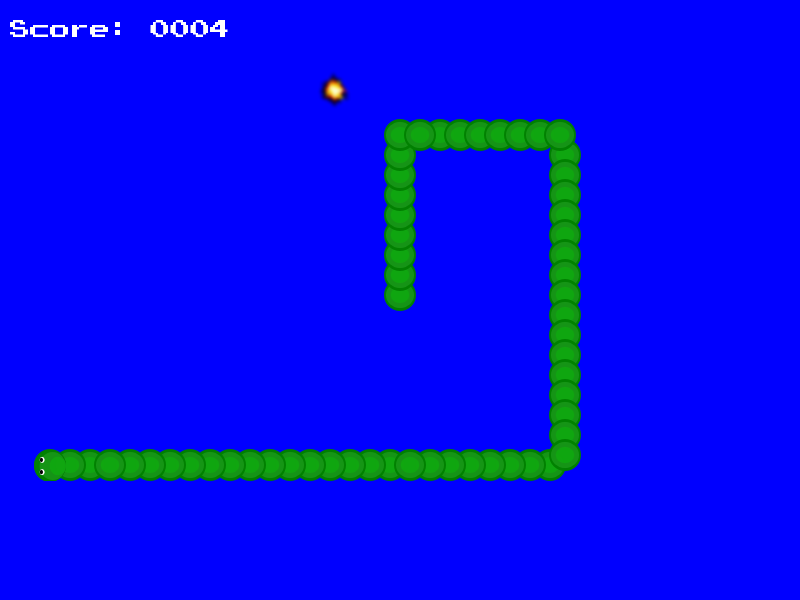
\includegraphics{ss-1-explode.png}
Clicking on the rock makes it go away but it doesn't really feel like it is exploding. Let's add a bit of animation to that by having an explosion occur.

Animations are just sprites that have a number of cells. Each cell of the animation will play for a certain length of time and then the animation will move on to the next cell. You can create cells of animation either from a single file or from multiple files. For this example we will use a single file where the cells of animation are arranged horizontally.

Here is our file.

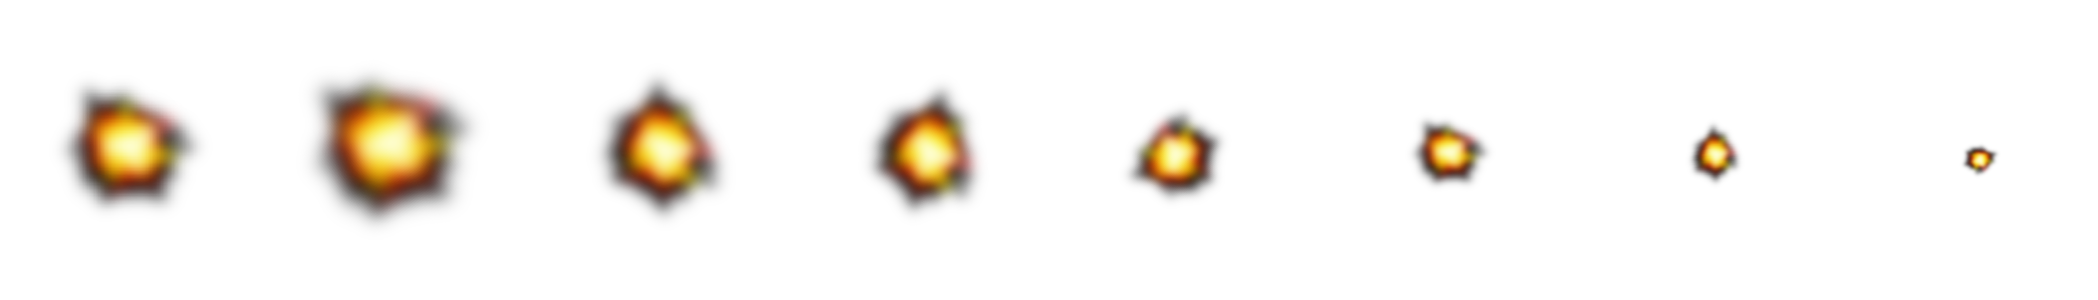
\includegraphics{explosion.png}

To register this as a sprite we use:

\begin{Verbatim}[commandchars=\\\{\},numbers=left,firstnumber=1,stepnumber=1]
\PYG{n}{serge}\PYG{o}{.}\PYG{n}{visual}\PYG{o}{.}\PYG{n}{Sprites}\PYG{o}{.}\PYG{n}{registerItem}\PYG{p}{(}\PYG{l+s}{'}\PYG{l+s}{explosion}\PYG{l+s}{'}\PYG{p}{,} \PYG{l+s}{'}\PYG{l+s}{explosion.png}\PYG{l+s}{'}\PYG{p}{,} \PYG{n}{zoom}\PYG{o}{=}\PYG{l+m+mf}{0.25}\PYG{p}{,}
    \PYG{n}{w}\PYG{o}{=}\PYG{l+m+mi}{8}\PYG{p}{,} \PYG{n}{framerate}\PYG{o}{=}\PYG{l+m+mi}{10}\PYG{p}{,} \PYG{n}{running}\PYG{o}{=}\PYG{n+nb+bp}{True}\PYG{p}{,} \PYG{n}{loop}\PYG{o}{=}\PYG{n+nb+bp}{False}\PYG{p}{,} \PYG{n}{one\PYGZus{}direction}\PYG{o}{=}\PYG{n+nb+bp}{True}\PYG{p}{)}
\end{Verbatim}

The framerate sets the number of cells that will be displayed per second. We do not want this animation to loop around and we only want it to go in one direction, ie we want it to run to the end of the animation and then stop. This particular graphic is actually quite large so we also use the \emph{zoom} argument to scale it down a bit.

We want to add the animation to the screen whenever we destroy a rock. There is a useful \emph{block} called an \emph{AnimateThenDie} actor that we can use for this purpose. This is an actor that we place in the world and it will run its animation one and then be removed. This actor is ideal for explosions because we just want them to show and then go away. Look in the \emph{destroyRock} method to see how we use this actor.

\begin{Verbatim}[commandchars=\\\{\},numbers=left,firstnumber=1,stepnumber=1]
\PYG{k+kn}{import} \PYG{n+nn}{random}
\PYG{k+kn}{import} \PYG{n+nn}{pygame}

\PYG{k+kn}{import} \PYG{n+nn}{serge.visual}
\PYG{k+kn}{import} \PYG{n+nn}{serge.sound}
\PYG{k+kn}{import} \PYG{n+nn}{serge.engine}
\PYG{k+kn}{import} \PYG{n+nn}{serge.actor}
\PYG{k+kn}{import} \PYG{n+nn}{serge.blocks.visualblocks}
\PYG{k+kn}{import} \PYG{n+nn}{serge.blocks.utils}
\PYG{k+kn}{import} \PYG{n+nn}{serge.blocks.directions}
\PYG{k+kn}{import} \PYG{n+nn}{serge.blocks.behaviours}
\PYG{k+kn}{import} \PYG{n+nn}{serge.blocks.actors}

\PYG{k}{class} \PYG{n+nc}{Snake}\PYG{p}{(}\PYG{n}{serge}\PYG{o}{.}\PYG{n}{actor}\PYG{o}{.}\PYG{n}{CompositeActor}\PYG{p}{)}\PYG{p}{:}
    \PYG{l+s+sd}{"""Represents the snake"""}

    \PYG{k}{def} \PYG{n+nf}{\PYGZus{}\PYGZus{}init\PYGZus{}\PYGZus{}}\PYG{p}{(}\PYG{n+nb+bp}{self}\PYG{p}{)}\PYG{p}{:}
        \PYG{l+s+sd}{"""Initialise the snake"""}
        \PYG{n+nb}{super}\PYG{p}{(}\PYG{n}{Snake}\PYG{p}{,} \PYG{n+nb+bp}{self}\PYG{p}{)}\PYG{o}{.}\PYG{n}{\PYGZus{}\PYGZus{}init\PYGZus{}\PYGZus{}}\PYG{p}{(}\PYG{l+s}{'}\PYG{l+s}{snake}\PYG{l+s}{'}\PYG{p}{,} \PYG{l+s}{'}\PYG{l+s}{snake-head}\PYG{l+s}{'}\PYG{p}{)}
        \PYG{n+nb+bp}{self}\PYG{o}{.}\PYG{n}{visual} \PYG{o}{=} \PYG{n}{serge}\PYG{o}{.}\PYG{n}{blocks}\PYG{o}{.}\PYG{n}{visualblocks}\PYG{o}{.}\PYG{n}{Circle}\PYG{p}{(}\PYG{l+m+mi}{16}\PYG{p}{,} \PYG{p}{(}\PYG{l+m+mi}{0}\PYG{p}{,}\PYG{l+m+mi}{255}\PYG{p}{,}\PYG{l+m+mi}{0}\PYG{p}{)}\PYG{p}{)}
        \PYG{n+nb+bp}{self}\PYG{o}{.}\PYG{n}{setSpriteName}\PYG{p}{(}\PYG{l+s}{'}\PYG{l+s}{head}\PYG{l+s}{'}\PYG{p}{)}
        \PYG{n+nb+bp}{self}\PYG{o}{.}\PYG{n}{setLayerName}\PYG{p}{(}\PYG{l+s}{'}\PYG{l+s}{middle}\PYG{l+s}{'}\PYG{p}{)}
        \PYG{n+nb+bp}{self}\PYG{o}{.}\PYG{n}{current\PYGZus{}direction} \PYG{o}{=} \PYG{n}{serge}\PYG{o}{.}\PYG{n}{blocks}\PYG{o}{.}\PYG{n}{directions}\PYG{o}{.}\PYG{n}{N}
        \PYG{n+nb+bp}{self}\PYG{o}{.}\PYG{n}{is\PYGZus{}dying} \PYG{o}{=} \PYG{n+nb+bp}{False}

    \PYG{k}{def} \PYG{n+nf}{addedToWorld}\PYG{p}{(}\PYG{n+nb+bp}{self}\PYG{p}{,} \PYG{n}{world}\PYG{p}{)}\PYG{p}{:}
        \PYG{l+s+sd}{"""The snake was added to the world"""}
        \PYG{n+nb}{super}\PYG{p}{(}\PYG{n}{Snake}\PYG{p}{,} \PYG{n+nb+bp}{self}\PYG{p}{)}\PYG{o}{.}\PYG{n}{addedToWorld}\PYG{p}{(}\PYG{n}{world}\PYG{p}{)}
        \PYG{c}{\PYGZsh{}}
        \PYG{n+nb+bp}{self}\PYG{o}{.}\PYG{n}{keyboard} \PYG{o}{=} \PYG{n}{serge}\PYG{o}{.}\PYG{n}{engine}\PYG{o}{.}\PYG{n}{CurrentEngine}\PYG{p}{(}\PYG{p}{)}\PYG{o}{.}\PYG{n}{getKeyboard}\PYG{p}{(}\PYG{p}{)}
        \PYG{n+nb+bp}{self}\PYG{o}{.}\PYG{n}{manager} \PYG{o}{=} \PYG{n}{serge}\PYG{o}{.}\PYG{n}{blocks}\PYG{o}{.}\PYG{n}{behaviours}\PYG{o}{.}\PYG{n}{BehaviourManager}\PYG{p}{(}\PYG{l+s}{'}\PYG{l+s}{manager}\PYG{l+s}{'}\PYG{p}{,} \PYG{l+s}{'}\PYG{l+s}{behaviour-manager}\PYG{l+s}{'}\PYG{p}{)}
        \PYG{n+nb+bp}{self}\PYG{o}{.}\PYG{n}{world} \PYG{o}{=} \PYG{n}{world}
        \PYG{n}{world}\PYG{o}{.}\PYG{n}{addActor}\PYG{p}{(}\PYG{n+nb+bp}{self}\PYG{o}{.}\PYG{n}{manager}\PYG{p}{)}
        \PYG{c}{\PYGZsh{}}
        \PYG{c}{\PYGZsh{} Text to display when the game is over}
        \PYG{n+nb+bp}{self}\PYG{o}{.}\PYG{n}{restart\PYGZus{}text} \PYG{o}{=} \PYG{n}{serge}\PYG{o}{.}\PYG{n}{blocks}\PYG{o}{.}\PYG{n}{utils}\PYG{o}{.}\PYG{n}{addVisualActorToWorld}\PYG{p}{(}\PYG{n}{world}\PYG{p}{,} \PYG{l+s}{'}\PYG{l+s}{text}\PYG{l+s}{'}\PYG{p}{,} \PYG{l+s}{'}\PYG{l+s}{restart}\PYG{l+s}{'}\PYG{p}{,}
            \PYG{n}{serge}\PYG{o}{.}\PYG{n}{visual}\PYG{o}{.}\PYG{n}{Text}\PYG{p}{(}\PYG{l+s}{'}\PYG{l+s}{Game Over - Press ENTER to restart}\PYG{l+s}{'}\PYG{p}{,} \PYG{p}{(}\PYG{l+m+mi}{255}\PYG{p}{,} \PYG{l+m+mi}{255}\PYG{p}{,} \PYG{l+m+mi}{255}\PYG{p}{)}\PYG{p}{,} \PYG{n}{font\PYGZus{}size}\PYG{o}{=}\PYG{l+m+mi}{20}\PYG{p}{)}\PYG{p}{,}
            \PYG{n}{layer\PYGZus{}name}\PYG{o}{=}\PYG{l+s}{'}\PYG{l+s}{front}\PYG{l+s}{'}\PYG{p}{,}
            \PYG{n}{center\PYGZus{}position}\PYG{o}{=}\PYG{p}{(}\PYG{l+m+mi}{400}\PYG{p}{,} \PYG{l+m+mi}{300}\PYG{p}{)}\PYG{p}{)}
        \PYG{n+nb+bp}{self}\PYG{o}{.}\PYG{n}{restart\PYGZus{}text}\PYG{o}{.}\PYG{n}{visible} \PYG{o}{=} \PYG{n+nb+bp}{False}
        \PYG{c}{\PYGZsh{}}
        \PYG{c}{\PYGZsh{} A background for the game}
        \PYG{n+nb+bp}{self}\PYG{o}{.}\PYG{n}{bg} \PYG{o}{=} \PYG{n}{serge}\PYG{o}{.}\PYG{n}{blocks}\PYG{o}{.}\PYG{n}{utils}\PYG{o}{.}\PYG{n}{addVisualActorToWorld}\PYG{p}{(}\PYG{n}{world}\PYG{p}{,} \PYG{l+s}{'}\PYG{l+s}{bg}\PYG{l+s}{'}\PYG{p}{,} \PYG{l+s}{'}\PYG{l+s}{bg}\PYG{l+s}{'}\PYG{p}{,}
            \PYG{n}{serge}\PYG{o}{.}\PYG{n}{blocks}\PYG{o}{.}\PYG{n}{visualblocks}\PYG{o}{.}\PYG{n}{Rectangle}\PYG{p}{(}\PYG{p}{(}\PYG{l+m+mi}{800}\PYG{p}{,} \PYG{l+m+mi}{600}\PYG{p}{)}\PYG{p}{,} \PYG{p}{(}\PYG{l+m+mi}{0}\PYG{p}{,}\PYG{l+m+mi}{0}\PYG{p}{,}\PYG{l+m+mi}{255}\PYG{p}{)}\PYG{p}{)}\PYG{p}{,}
            \PYG{n}{layer\PYGZus{}name}\PYG{o}{=}\PYG{l+s}{'}\PYG{l+s}{back}\PYG{l+s}{'}\PYG{p}{,}
            \PYG{n}{center\PYGZus{}position}\PYG{o}{=}\PYG{p}{(}\PYG{l+m+mi}{400}\PYG{p}{,} \PYG{l+m+mi}{300}\PYG{p}{)}\PYG{p}{)}
        \PYG{c}{\PYGZsh{}}
        \PYG{c}{\PYGZsh{} Text to show the score}
        \PYG{n+nb+bp}{self}\PYG{o}{.}\PYG{n}{score} \PYG{o}{=} \PYG{n}{serge}\PYG{o}{.}\PYG{n}{blocks}\PYG{o}{.}\PYG{n}{utils}\PYG{o}{.}\PYG{n}{addActorToWorld}\PYG{p}{(}\PYG{n}{world}\PYG{p}{,}
            \PYG{n}{serge}\PYG{o}{.}\PYG{n}{blocks}\PYG{o}{.}\PYG{n}{actors}\PYG{o}{.}\PYG{n}{NumericText}\PYG{p}{(}\PYG{l+s}{'}\PYG{l+s}{text}\PYG{l+s}{'}\PYG{p}{,} \PYG{l+s}{'}\PYG{l+s}{score}\PYG{l+s}{'}\PYG{p}{,} \PYG{l+s}{'}\PYG{l+s}{Score: }\PYG{l+s+si}{\PYGZpc{}04d}\PYG{l+s}{'}\PYG{p}{,}
                \PYG{p}{(}\PYG{l+m+mi}{255}\PYG{p}{,} \PYG{l+m+mi}{255}\PYG{p}{,} \PYG{l+m+mi}{255}\PYG{p}{)}\PYG{p}{,} \PYG{n}{font\PYGZus{}size}\PYG{o}{=}\PYG{l+m+mi}{20}\PYG{p}{,} \PYG{n}{font\PYGZus{}name}\PYG{o}{=}\PYG{l+s}{'}\PYG{l+s}{scores}\PYG{l+s}{'}\PYG{p}{,} \PYG{n}{value}\PYG{o}{=}\PYG{l+m+mi}{0}\PYG{p}{,} \PYG{n}{align}\PYG{o}{=}\PYG{l+s}{'}\PYG{l+s}{left}\PYG{l+s}{'}\PYG{p}{)}\PYG{p}{,}
            \PYG{n}{layer\PYGZus{}name}\PYG{o}{=}\PYG{l+s}{'}\PYG{l+s}{front}\PYG{l+s}{'}\PYG{p}{,}
            \PYG{n}{center\PYGZus{}position}\PYG{o}{=}\PYG{p}{(}\PYG{l+m+mi}{120}\PYG{p}{,} \PYG{l+m+mi}{30}\PYG{p}{)}\PYG{p}{)}

    \PYG{k}{def} \PYG{n+nf}{updateActor}\PYG{p}{(}\PYG{n+nb+bp}{self}\PYG{p}{,} \PYG{n}{interval}\PYG{p}{,} \PYG{n}{world}\PYG{p}{)}\PYG{p}{:}
        \PYG{l+s+sd}{"""Update the snake"""}
        \PYG{n+nb}{super}\PYG{p}{(}\PYG{n}{Snake}\PYG{p}{,} \PYG{n+nb+bp}{self}\PYG{p}{)}\PYG{o}{.}\PYG{n}{updateActor}\PYG{p}{(}\PYG{n}{interval}\PYG{p}{,} \PYG{n}{world}\PYG{p}{)}
        \PYG{c}{\PYGZsh{}}
        \PYG{c}{\PYGZsh{} Quit if requested}
        \PYG{k}{if} \PYG{n+nb+bp}{self}\PYG{o}{.}\PYG{n}{keyboard}\PYG{o}{.}\PYG{n}{isClicked}\PYG{p}{(}\PYG{n}{pygame}\PYG{o}{.}\PYG{n}{K\PYGZus{}ESCAPE}\PYG{p}{)}\PYG{p}{:}
            \PYG{n}{serge}\PYG{o}{.}\PYG{n}{engine}\PYG{o}{.}\PYG{n}{CurrentEngine}\PYG{p}{(}\PYG{p}{)}\PYG{o}{.}\PYG{n}{stop}\PYG{p}{(}\PYG{p}{)}
        \PYG{c}{\PYGZsh{}}
        \PYG{c}{\PYGZsh{} Move the head}
        \PYG{k}{if} \PYG{n+nb+bp}{self}\PYG{o}{.}\PYG{n}{keyboard}\PYG{o}{.}\PYG{n}{isClicked}\PYG{p}{(}\PYG{n}{pygame}\PYG{o}{.}\PYG{n}{K\PYGZus{}LEFT}\PYG{p}{)}\PYG{p}{:}
            \PYG{n}{rotation} \PYG{o}{=} \PYG{o}{+}\PYG{l+m+mi}{90}
        \PYG{k}{elif} \PYG{n+nb+bp}{self}\PYG{o}{.}\PYG{n}{keyboard}\PYG{o}{.}\PYG{n}{isClicked}\PYG{p}{(}\PYG{n}{pygame}\PYG{o}{.}\PYG{n}{K\PYGZus{}RIGHT}\PYG{p}{)}\PYG{p}{:}
            \PYG{n}{rotation} \PYG{o}{=} \PYG{o}{-}\PYG{l+m+mi}{90}
        \PYG{k}{else}\PYG{p}{:}
            \PYG{n}{rotation} \PYG{o}{=} \PYG{l+m+mi}{0}
        \PYG{c}{\PYGZsh{}}
        \PYG{c}{\PYGZsh{} Change direction}
        \PYG{k}{if} \PYG{n}{rotation}\PYG{p}{:}
            \PYG{n}{current\PYGZus{}angle} \PYG{o}{=} \PYG{n}{serge}\PYG{o}{.}\PYG{n}{blocks}\PYG{o}{.}\PYG{n}{directions}\PYG{o}{.}\PYG{n}{getAngleFromCardinal}\PYG{p}{(}\PYG{n+nb+bp}{self}\PYG{o}{.}\PYG{n}{current\PYGZus{}direction}\PYG{p}{)}
            \PYG{n+nb+bp}{self}\PYG{o}{.}\PYG{n}{current\PYGZus{}direction} \PYG{o}{=} \PYG{n}{serge}\PYG{o}{.}\PYG{n}{blocks}\PYG{o}{.}\PYG{n}{directions}\PYG{o}{.}\PYG{n}{getCardinalFromAngle}\PYG{p}{(}\PYG{n}{current\PYGZus{}angle}\PYG{o}{+}\PYG{n}{rotation}\PYG{p}{)}
            \PYG{n+nb+bp}{self}\PYG{o}{.}\PYG{n}{visual}\PYG{o}{.}\PYG{n}{setAngle}\PYG{p}{(}\PYG{n}{current\PYGZus{}angle}\PYG{o}{+}\PYG{n}{rotation}\PYG{p}{)}
        \PYG{c}{\PYGZsh{}}
        \PYG{c}{\PYGZsh{} Move}
        \PYG{k}{if} \PYG{o+ow}{not} \PYG{n+nb+bp}{self}\PYG{o}{.}\PYG{n}{is\PYGZus{}dying}\PYG{p}{:}
            \PYG{n}{offset} \PYG{o}{=} \PYG{l+m+mi}{5}\PYG{o}{*}\PYG{n}{serge}\PYG{o}{.}\PYG{n}{blocks}\PYG{o}{.}\PYG{n}{directions}\PYG{o}{.}\PYG{n}{getVectorFromCardinal}\PYG{p}{(}\PYG{n+nb+bp}{self}\PYG{o}{.}\PYG{n}{current\PYGZus{}direction}\PYG{p}{)}
            \PYG{n+nb+bp}{self}\PYG{o}{.}\PYG{n}{move}\PYG{p}{(}\PYG{o}{*}\PYG{n}{offset}\PYG{p}{)}
            \PYG{c}{\PYGZsh{}}
            \PYG{c}{\PYGZsh{} Adding random rocks}
            \PYG{k}{if} \PYG{n}{random}\PYG{o}{.}\PYG{n}{random}\PYG{p}{(}\PYG{p}{)} \PYG{o}{\textless{}} \PYG{l+m+mf}{0.01}\PYG{p}{:}
                \PYG{n+nb+bp}{self}\PYG{o}{.}\PYG{n}{addRock}\PYG{p}{(}\PYG{p}{)}
            \PYG{c}{\PYGZsh{}}
            \PYG{c}{\PYGZsh{} Add a new segment if needed}
            \PYG{k}{if} \PYG{o+ow}{not} \PYG{n+nb+bp}{self}\PYG{o}{.}\PYG{n}{getChildren}\PYG{p}{(}\PYG{p}{)} \PYG{o+ow}{or} \PYG{n+nb+bp}{self}\PYG{o}{.}\PYG{n}{getDistanceFrom}\PYG{p}{(}\PYG{n+nb+bp}{self}\PYG{o}{.}\PYG{n}{getChildren}\PYG{p}{(}\PYG{p}{)}\PYG{p}{[}\PYG{o}{-}\PYG{l+m+mi}{1}\PYG{p}{]}\PYG{p}{)} \PYG{o}{\textgreater{}} \PYG{l+m+mi}{16}\PYG{p}{:}
                \PYG{n+nb+bp}{self}\PYG{o}{.}\PYG{n}{addSegment}\PYG{p}{(}\PYG{p}{)}
            \PYG{c}{\PYGZsh{}}
            \PYG{c}{\PYGZsh{} Check if we hit the body}
            \PYG{k}{if} \PYG{n+nb+bp}{self}\PYG{o}{.}\PYG{n}{hitBody}\PYG{p}{(}\PYG{p}{)} \PYG{o+ow}{or} \PYG{n+nb+bp}{self}\PYG{o}{.}\PYG{n}{offScreen}\PYG{p}{(}\PYG{p}{)} \PYG{o+ow}{or} \PYG{n+nb+bp}{self}\PYG{o}{.}\PYG{n}{hitRock}\PYG{p}{(}\PYG{p}{)}\PYG{p}{:}
                \PYG{n+nb+bp}{self}\PYG{o}{.}\PYG{n}{initiateDeathAnimation}\PYG{p}{(}\PYG{p}{)}
            \PYG{c}{\PYGZsh{}}
            \PYG{c}{\PYGZsh{} Increase score}
            \PYG{n+nb+bp}{self}\PYG{o}{.}\PYG{n}{score}\PYG{o}{.}\PYG{n}{value} \PYG{o}{+}\PYG{o}{=} \PYG{n}{interval}\PYG{o}{/}\PYG{l+m+mf}{1000.0}
        \PYG{k}{elif} \PYG{n+nb+bp}{self}\PYG{o}{.}\PYG{n}{animation}\PYG{o}{.}\PYG{n}{isComplete}\PYG{p}{(}\PYG{p}{)}\PYG{p}{:}
            \PYG{k}{if} \PYG{n+nb+bp}{self}\PYG{o}{.}\PYG{n}{keyboard}\PYG{o}{.}\PYG{n}{isClicked}\PYG{p}{(}\PYG{n}{pygame}\PYG{o}{.}\PYG{n}{K\PYGZus{}KP\PYGZus{}ENTER}\PYG{p}{)} \PYG{o+ow}{or} \PYG{n+nb+bp}{self}\PYG{o}{.}\PYG{n}{keyboard}\PYG{o}{.}\PYG{n}{isClicked}\PYG{p}{(}\PYG{n}{pygame}\PYG{o}{.}\PYG{n}{K\PYGZus{}RETURN}\PYG{p}{)}\PYG{p}{:}
                \PYG{n+nb+bp}{self}\PYG{o}{.}\PYG{n}{restartGame}\PYG{p}{(}\PYG{p}{)}

    \PYG{k}{def} \PYG{n+nf}{addSegment}\PYG{p}{(}\PYG{n+nb+bp}{self}\PYG{p}{)}\PYG{p}{:}
        \PYG{l+s+sd}{"""Add a new body segment"""}
        \PYG{n}{segment} \PYG{o}{=} \PYG{n}{serge}\PYG{o}{.}\PYG{n}{actor}\PYG{o}{.}\PYG{n}{Actor}\PYG{p}{(}\PYG{l+s}{'}\PYG{l+s}{segment}\PYG{l+s}{'}\PYG{p}{)}
        \PYG{n}{segment}\PYG{o}{.}\PYG{n}{setSpriteName}\PYG{p}{(}\PYG{l+s}{'}\PYG{l+s}{tail}\PYG{l+s}{'}\PYG{p}{)}
        \PYG{n}{segment}\PYG{o}{.}\PYG{n}{setLayerName}\PYG{p}{(}\PYG{l+s}{'}\PYG{l+s}{middle}\PYG{l+s}{'}\PYG{p}{)}
        \PYG{n}{segment}\PYG{o}{.}\PYG{n}{moveTo}\PYG{p}{(}\PYG{n+nb+bp}{self}\PYG{o}{.}\PYG{n}{x}\PYG{p}{,} \PYG{n+nb+bp}{self}\PYG{o}{.}\PYG{n}{y}\PYG{p}{)}
        \PYG{n+nb+bp}{self}\PYG{o}{.}\PYG{n}{addChild}\PYG{p}{(}\PYG{n}{segment}\PYG{p}{)}
        \PYG{n}{serge}\PYG{o}{.}\PYG{n}{sound}\PYG{o}{.}\PYG{n}{Sounds}\PYG{o}{.}\PYG{n}{play}\PYG{p}{(}\PYG{l+s}{'}\PYG{l+s}{new-body}\PYG{l+s}{'}\PYG{p}{)}

    \PYG{k}{def} \PYG{n+nf}{addRock}\PYG{p}{(}\PYG{n+nb+bp}{self}\PYG{p}{)}\PYG{p}{:}
        \PYG{l+s+sd}{"""Add a rock to the screen"""}
        \PYG{n}{position} \PYG{o}{=} \PYG{p}{(}\PYG{n}{random}\PYG{o}{.}\PYG{n}{randrange}\PYG{p}{(}\PYG{l+m+mi}{0}\PYG{p}{,} \PYG{l+m+mi}{800}\PYG{p}{)}\PYG{p}{,} \PYG{n}{random}\PYG{o}{.}\PYG{n}{randrange}\PYG{p}{(}\PYG{l+m+mi}{0}\PYG{p}{,} \PYG{l+m+mi}{600}\PYG{p}{)}\PYG{p}{)}
        \PYG{n}{rock} \PYG{o}{=} \PYG{n}{serge}\PYG{o}{.}\PYG{n}{actor}\PYG{o}{.}\PYG{n}{Actor}\PYG{p}{(}\PYG{l+s}{'}\PYG{l+s}{rock}\PYG{l+s}{'}\PYG{p}{)}
        \PYG{n}{rock}\PYG{o}{.}\PYG{n}{setSpriteName}\PYG{p}{(}\PYG{l+s}{'}\PYG{l+s}{rock}\PYG{l+s}{'}\PYG{p}{)}
        \PYG{n}{rock}\PYG{o}{.}\PYG{n}{setLayerName}\PYG{p}{(}\PYG{l+s}{'}\PYG{l+s}{middle}\PYG{l+s}{'}\PYG{p}{)}
        \PYG{n}{rock}\PYG{o}{.}\PYG{n}{moveTo}\PYG{p}{(}\PYG{o}{*}\PYG{n}{position}\PYG{p}{)}
        \PYG{n}{rock}\PYG{o}{.}\PYG{n}{setAngle}\PYG{p}{(}\PYG{n}{random}\PYG{o}{.}\PYG{n}{randrange}\PYG{p}{(}\PYG{l+m+mi}{0}\PYG{p}{,} \PYG{l+m+mi}{360}\PYG{p}{)}\PYG{p}{)}
        \PYG{n}{rock}\PYG{o}{.}\PYG{n}{linkEvent}\PYG{p}{(}\PYG{n}{serge}\PYG{o}{.}\PYG{n}{events}\PYG{o}{.}\PYG{n}{E\PYGZus{}LEFT\PYGZus{}CLICK}\PYG{p}{,} \PYG{n+nb+bp}{self}\PYG{o}{.}\PYG{n}{destroyRock}\PYG{p}{,} \PYG{n}{rock}\PYG{p}{)}
        \PYG{n+nb+bp}{self}\PYG{o}{.}\PYG{n}{world}\PYG{o}{.}\PYG{n}{addActor}\PYG{p}{(}\PYG{n}{rock}\PYG{p}{)}

    \PYG{k}{def} \PYG{n+nf}{hitBody}\PYG{p}{(}\PYG{n+nb+bp}{self}\PYG{p}{)}\PYG{p}{:}
        \PYG{l+s+sd}{"""Return True if the head has hit the body}

\PYG{l+s+sd}{        Look to see if we overlap with any body segment except the last}
\PYG{l+s+sd}{        (we are allowed to overlap the last since we just put it down)}

\PYG{l+s+sd}{        """}
        \PYG{k}{for} \PYG{n}{segment} \PYG{o+ow}{in} \PYG{n+nb+bp}{self}\PYG{o}{.}\PYG{n}{getChildren}\PYG{p}{(}\PYG{p}{)}\PYG{p}{[}\PYG{p}{:}\PYG{o}{-}\PYG{l+m+mi}{1}\PYG{p}{]}\PYG{p}{:}
            \PYG{k}{if} \PYG{n+nb+bp}{self}\PYG{o}{.}\PYG{n}{getDistanceFrom}\PYG{p}{(}\PYG{n}{segment}\PYG{p}{)} \PYG{o}{\textless{}} \PYG{l+m+mi}{16}\PYG{p}{:}
                \PYG{k}{return} \PYG{n+nb+bp}{True}
        \PYG{k}{return} \PYG{n+nb+bp}{False}

    \PYG{k}{def} \PYG{n+nf}{hitRock}\PYG{p}{(}\PYG{n+nb+bp}{self}\PYG{p}{)}\PYG{p}{:}
        \PYG{l+s+sd}{"""Return True if we hit a rock"""}
        \PYG{k}{for} \PYG{n}{rock} \PYG{o+ow}{in} \PYG{n+nb+bp}{self}\PYG{o}{.}\PYG{n}{world}\PYG{o}{.}\PYG{n}{findActorsByTag}\PYG{p}{(}\PYG{l+s}{'}\PYG{l+s}{rock}\PYG{l+s}{'}\PYG{p}{)}\PYG{p}{:}
            \PYG{k}{if} \PYG{n+nb+bp}{self}\PYG{o}{.}\PYG{n}{getDistanceFrom}\PYG{p}{(}\PYG{n}{rock}\PYG{p}{)} \PYG{o}{\textless{}} \PYG{l+m+mi}{16}\PYG{p}{:}
                \PYG{k}{return} \PYG{n+nb+bp}{True}
        \PYG{k}{else}\PYG{p}{:}
            \PYG{k}{return} \PYG{n+nb+bp}{False}

    \PYG{k}{def} \PYG{n+nf}{offScreen}\PYG{p}{(}\PYG{n+nb+bp}{self}\PYG{p}{)}\PYG{p}{:}
        \PYG{l+s+sd}{"""Return True if we are off the screen"""}
        \PYG{k}{return} \PYG{n+nb+bp}{self}\PYG{o}{.}\PYG{n}{x} \PYG{o}{\textless{}} \PYG{l+m+mi}{0} \PYG{o+ow}{or} \PYG{n+nb+bp}{self}\PYG{o}{.}\PYG{n}{x} \PYG{o}{\textgreater{}} \PYG{l+m+mi}{800} \PYG{o+ow}{or} \PYG{n+nb+bp}{self}\PYG{o}{.}\PYG{n}{y} \PYG{o}{\textless{}} \PYG{l+m+mi}{0} \PYG{o+ow}{or} \PYG{n+nb+bp}{self}\PYG{o}{.}\PYG{n}{y} \PYG{o}{\textgreater{}} \PYG{l+m+mi}{600}

    \PYG{k}{def} \PYG{n+nf}{initiateDeathAnimation}\PYG{p}{(}\PYG{n+nb+bp}{self}\PYG{p}{)}\PYG{p}{:}
        \PYG{l+s+sd}{"""Begin showing the death of the snake"""}
        \PYG{n+nb+bp}{self}\PYG{o}{.}\PYG{n}{log}\PYG{o}{.}\PYG{n}{info}\PYG{p}{(}\PYG{l+s}{'}\PYG{l+s}{Snake died!}\PYG{l+s}{'}\PYG{p}{)}
        \PYG{n+nb+bp}{self}\PYG{o}{.}\PYG{n}{animation} \PYG{o}{=} \PYG{n+nb+bp}{self}\PYG{o}{.}\PYG{n}{manager}\PYG{o}{.}\PYG{n}{assignBehaviour}\PYG{p}{(}\PYG{n+nb+bp}{self}\PYG{p}{,}
            \PYG{n}{serge}\PYG{o}{.}\PYG{n}{blocks}\PYG{o}{.}\PYG{n}{behaviours}\PYG{o}{.}\PYG{n}{TimedCallback}\PYG{p}{(}\PYG{l+m+mi}{1000}\PYG{o}{/}\PYG{n+nb}{len}\PYG{p}{(}\PYG{n+nb+bp}{self}\PYG{o}{.}\PYG{n}{getChildren}\PYG{p}{(}\PYG{p}{)}\PYG{p}{)}\PYG{p}{,} \PYG{n+nb+bp}{self}\PYG{o}{.}\PYG{n}{removeTail}\PYG{p}{)}\PYG{p}{,} \PYG{l+s}{'}\PYG{l+s}{death-animation}\PYG{l+s}{'}\PYG{p}{)}
        \PYG{n+nb+bp}{self}\PYG{o}{.}\PYG{n}{is\PYGZus{}dying} \PYG{o}{=} \PYG{n+nb+bp}{True}
        \PYG{k}{for} \PYG{n}{segment} \PYG{o+ow}{in} \PYG{n+nb+bp}{self}\PYG{o}{.}\PYG{n}{getChildren}\PYG{p}{(}\PYG{p}{)}\PYG{p}{:}
            \PYG{n}{segment}\PYG{o}{.}\PYG{n}{setSpriteName}\PYG{p}{(}\PYG{l+s}{'}\PYG{l+s}{red-tail}\PYG{l+s}{'}\PYG{p}{)}
        \PYG{n+nb+bp}{self}\PYG{o}{.}\PYG{n}{setSpriteName}\PYG{p}{(}\PYG{l+s}{'}\PYG{l+s}{red-head}\PYG{l+s}{'}\PYG{p}{)}
        \PYG{n}{serge}\PYG{o}{.}\PYG{n}{sound}\PYG{o}{.}\PYG{n}{Sounds}\PYG{o}{.}\PYG{n}{play}\PYG{p}{(}\PYG{l+s}{'}\PYG{l+s}{snake-death}\PYG{l+s}{'}\PYG{p}{)}

    \PYG{k}{def} \PYG{n+nf}{removeTail}\PYG{p}{(}\PYG{n+nb+bp}{self}\PYG{p}{,} \PYG{n}{world}\PYG{p}{,} \PYG{n}{actor}\PYG{p}{,} \PYG{n}{interval}\PYG{p}{)}\PYG{p}{:}
        \PYG{l+s+sd}{"""Remove part of the tail"""}
        \PYG{n+nb+bp}{self}\PYG{o}{.}\PYG{n}{log}\PYG{o}{.}\PYG{n}{debug}\PYG{p}{(}\PYG{l+s}{'}\PYG{l+s}{Removing part of the tail}\PYG{l+s}{'}\PYG{p}{)}
        \PYG{k}{if} \PYG{n+nb+bp}{self}\PYG{o}{.}\PYG{n}{getChildren}\PYG{p}{(}\PYG{p}{)}\PYG{p}{:}
            \PYG{n+nb+bp}{self}\PYG{o}{.}\PYG{n}{removeChild}\PYG{p}{(}\PYG{n+nb+bp}{self}\PYG{o}{.}\PYG{n}{getChildren}\PYG{p}{(}\PYG{p}{)}\PYG{p}{[}\PYG{l+m+mi}{0}\PYG{p}{]}\PYG{p}{)}
        \PYG{k}{else}\PYG{p}{:}
            \PYG{n+nb+bp}{self}\PYG{o}{.}\PYG{n}{animation}\PYG{o}{.}\PYG{n}{markComplete}\PYG{p}{(}\PYG{p}{)}
            \PYG{n+nb+bp}{self}\PYG{o}{.}\PYG{n}{restart\PYGZus{}text}\PYG{o}{.}\PYG{n}{visible} \PYG{o}{=} \PYG{n+nb+bp}{True}
            \PYG{n}{serge}\PYG{o}{.}\PYG{n}{sound}\PYG{o}{.}\PYG{n}{Sounds}\PYG{o}{.}\PYG{n}{getItem}\PYG{p}{(}\PYG{l+s}{'}\PYG{l+s}{snake-death}\PYG{l+s}{'}\PYG{p}{)}\PYG{o}{.}\PYG{n}{fadeout}\PYG{p}{(}\PYG{l+m+mi}{500}\PYG{p}{)}

    \PYG{k}{def} \PYG{n+nf}{destroyRock}\PYG{p}{(}\PYG{n+nb+bp}{self}\PYG{p}{,} \PYG{n}{obj}\PYG{p}{,} \PYG{n}{rock}\PYG{p}{)}\PYG{p}{:}
        \PYG{l+s+sd}{"""Destroy a rock"""}
        \PYG{n+nb+bp}{self}\PYG{o}{.}\PYG{n}{world}\PYG{o}{.}\PYG{n}{removeActor}\PYG{p}{(}\PYG{n}{rock}\PYG{p}{)}
        \PYG{n}{explosion} \PYG{o}{=} \PYG{n}{serge}\PYG{o}{.}\PYG{n}{blocks}\PYG{o}{.}\PYG{n}{actors}\PYG{o}{.}\PYG{n}{AnimateThenDieActor}\PYG{p}{(}\PYG{l+s}{'}\PYG{l+s}{explosion}\PYG{l+s}{'}\PYG{p}{,} \PYG{l+s}{'}\PYG{l+s}{explosion}\PYG{l+s}{'}\PYG{p}{,} \PYG{l+s}{'}\PYG{l+s}{explosion}\PYG{l+s}{'}\PYG{p}{,} \PYG{l+s}{'}\PYG{l+s}{front}\PYG{l+s}{'}\PYG{p}{)}
        \PYG{n}{explosion}\PYG{o}{.}\PYG{n}{moveTo}\PYG{p}{(}\PYG{n}{rock}\PYG{o}{.}\PYG{n}{x}\PYG{p}{,} \PYG{n}{rock}\PYG{o}{.}\PYG{n}{y}\PYG{p}{)}
        \PYG{n+nb+bp}{self}\PYG{o}{.}\PYG{n}{world}\PYG{o}{.}\PYG{n}{addActor}\PYG{p}{(}\PYG{n}{explosion}\PYG{p}{)}

    \PYG{k}{def} \PYG{n+nf}{restartGame}\PYG{p}{(}\PYG{n+nb+bp}{self}\PYG{p}{)}\PYG{p}{:}
        \PYG{l+s+sd}{"""Restart the game"""}
        \PYG{n+nb+bp}{self}\PYG{o}{.}\PYG{n}{is\PYGZus{}dying} \PYG{o}{=} \PYG{n+nb+bp}{False}
        \PYG{n+nb+bp}{self}\PYG{o}{.}\PYG{n}{restart\PYGZus{}text}\PYG{o}{.}\PYG{n}{visible} \PYG{o}{=} \PYG{n+nb+bp}{False}
        \PYG{n+nb+bp}{self}\PYG{o}{.}\PYG{n}{setSpriteName}\PYG{p}{(}\PYG{l+s}{'}\PYG{l+s}{head}\PYG{l+s}{'}\PYG{p}{)}
        \PYG{n+nb+bp}{self}\PYG{o}{.}\PYG{n}{current\PYGZus{}direction} \PYG{o}{=} \PYG{n}{serge}\PYG{o}{.}\PYG{n}{blocks}\PYG{o}{.}\PYG{n}{directions}\PYG{o}{.}\PYG{n}{N}
        \PYG{n+nb+bp}{self}\PYG{o}{.}\PYG{n}{score}\PYG{o}{.}\PYG{n}{value} \PYG{o}{=} \PYG{l+m+mi}{0}
        \PYG{n+nb+bp}{self}\PYG{o}{.}\PYG{n}{moveTo}\PYG{p}{(}\PYG{l+m+mi}{400}\PYG{p}{,} \PYG{l+m+mi}{300}\PYG{p}{)}
        \PYG{n+nb+bp}{self}\PYG{o}{.}\PYG{n}{world}\PYG{o}{.}\PYG{n}{clearActorsWithTags}\PYG{p}{(}\PYG{p}{[}\PYG{l+s}{'}\PYG{l+s}{rock}\PYG{l+s}{'}\PYG{p}{]}\PYG{p}{)}


\PYG{c}{\PYGZsh{} Create the engine}
\PYG{n}{engine} \PYG{o}{=} \PYG{n}{serge}\PYG{o}{.}\PYG{n}{blocks}\PYG{o}{.}\PYG{n}{utils}\PYG{o}{.}\PYG{n}{getSimpleSetup}\PYG{p}{(}\PYG{l+m+mi}{800}\PYG{p}{,} \PYG{l+m+mi}{600}\PYG{p}{)}
\PYG{n}{world} \PYG{o}{=} \PYG{n}{engine}\PYG{o}{.}\PYG{n}{getWorld}\PYG{p}{(}\PYG{l+s}{'}\PYG{l+s}{lab}\PYG{l+s}{'}\PYG{p}{)}

\PYG{c}{\PYGZsh{} Register sprites}
\PYG{n}{serge}\PYG{o}{.}\PYG{n}{visual}\PYG{o}{.}\PYG{n}{Sprites}\PYG{o}{.}\PYG{n}{setPath}\PYG{p}{(}\PYG{l+s}{'}\PYG{l+s}{graphics}\PYG{l+s}{'}\PYG{p}{)}
\PYG{n}{serge}\PYG{o}{.}\PYG{n}{visual}\PYG{o}{.}\PYG{n}{Sprites}\PYG{o}{.}\PYG{n}{registerItem}\PYG{p}{(}\PYG{l+s}{'}\PYG{l+s}{head}\PYG{l+s}{'}\PYG{p}{,} \PYG{l+s}{'}\PYG{l+s}{head.png}\PYG{l+s}{'}\PYG{p}{)}
\PYG{n}{serge}\PYG{o}{.}\PYG{n}{visual}\PYG{o}{.}\PYG{n}{Sprites}\PYG{o}{.}\PYG{n}{registerItem}\PYG{p}{(}\PYG{l+s}{'}\PYG{l+s}{tail}\PYG{l+s}{'}\PYG{p}{,} \PYG{l+s}{'}\PYG{l+s}{tail.png}\PYG{l+s}{'}\PYG{p}{)}
\PYG{n}{serge}\PYG{o}{.}\PYG{n}{visual}\PYG{o}{.}\PYG{n}{Sprites}\PYG{o}{.}\PYG{n}{registerItem}\PYG{p}{(}\PYG{l+s}{'}\PYG{l+s}{red-head}\PYG{l+s}{'}\PYG{p}{,} \PYG{l+s}{'}\PYG{l+s}{red-head.png}\PYG{l+s}{'}\PYG{p}{)}
\PYG{n}{serge}\PYG{o}{.}\PYG{n}{visual}\PYG{o}{.}\PYG{n}{Sprites}\PYG{o}{.}\PYG{n}{registerItem}\PYG{p}{(}\PYG{l+s}{'}\PYG{l+s}{red-tail}\PYG{l+s}{'}\PYG{p}{,} \PYG{l+s}{'}\PYG{l+s}{red-tail.png}\PYG{l+s}{'}\PYG{p}{)}
\PYG{n}{serge}\PYG{o}{.}\PYG{n}{visual}\PYG{o}{.}\PYG{n}{Sprites}\PYG{o}{.}\PYG{n}{registerItem}\PYG{p}{(}\PYG{l+s}{'}\PYG{l+s}{rock}\PYG{l+s}{'}\PYG{p}{,} \PYG{l+s}{'}\PYG{l+s}{rock.png}\PYG{l+s}{'}\PYG{p}{)}
\PYG{n}{serge}\PYG{o}{.}\PYG{n}{visual}\PYG{o}{.}\PYG{n}{Sprites}\PYG{o}{.}\PYG{n}{registerItem}\PYG{p}{(}\PYG{l+s}{'}\PYG{l+s}{explosion}\PYG{l+s}{'}\PYG{p}{,} \PYG{l+s}{'}\PYG{l+s}{explosion.png}\PYG{l+s}{'}\PYG{p}{,} \PYG{n}{zoom}\PYG{o}{=}\PYG{l+m+mf}{0.25}\PYG{p}{,}
        \PYG{n}{w}\PYG{o}{=}\PYG{l+m+mi}{8}\PYG{p}{,} \PYG{n}{framerate}\PYG{o}{=}\PYG{l+m+mi}{10}\PYG{p}{,} \PYG{n}{running}\PYG{o}{=}\PYG{n+nb+bp}{True}\PYG{p}{,} \PYG{n}{loop}\PYG{o}{=}\PYG{n+nb+bp}{False}\PYG{p}{,} \PYG{n}{one\PYGZus{}direction}\PYG{o}{=}\PYG{n+nb+bp}{True}\PYG{p}{)}

\PYG{c}{\PYGZsh{} Register sounds}
\PYG{n}{serge}\PYG{o}{.}\PYG{n}{sound}\PYG{o}{.}\PYG{n}{Sounds}\PYG{o}{.}\PYG{n}{setPath}\PYG{p}{(}\PYG{l+s}{'}\PYG{l+s}{sounds}\PYG{l+s}{'}\PYG{p}{)}
\PYG{n}{serge}\PYG{o}{.}\PYG{n}{sound}\PYG{o}{.}\PYG{n}{Sounds}\PYG{o}{.}\PYG{n}{registerItem}\PYG{p}{(}\PYG{l+s}{'}\PYG{l+s}{new-body}\PYG{l+s}{'}\PYG{p}{,} \PYG{l+s}{'}\PYG{l+s}{bloop.wav}\PYG{l+s}{'}\PYG{p}{)}
\PYG{n}{serge}\PYG{o}{.}\PYG{n}{sound}\PYG{o}{.}\PYG{n}{Sounds}\PYG{o}{.}\PYG{n}{registerItem}\PYG{p}{(}\PYG{l+s}{'}\PYG{l+s}{snake-death}\PYG{l+s}{'}\PYG{p}{,} \PYG{l+s}{'}\PYG{l+s}{death.wav}\PYG{l+s}{'}\PYG{p}{)}

\PYG{c}{\PYGZsh{} Register fonts}
\PYG{n}{serge}\PYG{o}{.}\PYG{n}{visual}\PYG{o}{.}\PYG{n}{Fonts}\PYG{o}{.}\PYG{n}{setPath}\PYG{p}{(}\PYG{l+s}{'}\PYG{l+s}{fonts}\PYG{l+s}{'}\PYG{p}{)}
\PYG{n}{serge}\PYG{o}{.}\PYG{n}{visual}\PYG{o}{.}\PYG{n}{Fonts}\PYG{o}{.}\PYG{n}{registerItem}\PYG{p}{(}\PYG{l+s}{'}\PYG{l+s}{DEFAULT}\PYG{l+s}{'}\PYG{p}{,} \PYG{l+s}{'}\PYG{l+s}{MedievalSharp.ttf}\PYG{l+s}{'}\PYG{p}{)}
\PYG{n}{serge}\PYG{o}{.}\PYG{n}{visual}\PYG{o}{.}\PYG{n}{Fonts}\PYG{o}{.}\PYG{n}{registerItem}\PYG{p}{(}\PYG{l+s}{'}\PYG{l+s}{scores}\PYG{l+s}{'}\PYG{p}{,} \PYG{l+s}{'}\PYG{l+s}{PressStart2P.ttf}\PYG{l+s}{'}\PYG{p}{)}

\PYG{c}{\PYGZsh{} Create the snake}
\PYG{n}{snake} \PYG{o}{=} \PYG{n}{Snake}\PYG{p}{(}\PYG{p}{)}
\PYG{n}{world}\PYG{o}{.}\PYG{n}{addActor}\PYG{p}{(}\PYG{n}{snake}\PYG{p}{)}
\PYG{n}{snake}\PYG{o}{.}\PYG{n}{moveTo}\PYG{p}{(}\PYG{l+m+mi}{400}\PYG{p}{,} \PYG{l+m+mi}{300}\PYG{p}{)}

\PYG{c}{\PYGZsh{} Run the game}
\PYG{n}{engine}\PYG{o}{.}\PYG{n}{run}\PYG{p}{(}\PYG{l+m+mi}{60}\PYG{p}{)}
\end{Verbatim}


\subsection{Conclusion}
\label{tutorial-2:conclusion}
This concludes the snake tutorial. We have the basics of a playable game and covered the main fundamental concepts. We covered the following classes - take a look at their detailed documentation.
\begin{itemize}
\item {} 
{\hyperref[engine:module-engine]{\code{The Engine}}}

\item {} 
{\hyperref[world:module-world]{\code{Worlds}}}

\item {} 
{\hyperref[actor:module-actor]{\code{Actors}}}

\item {} 
{\hyperref[visual:module-visual]{\code{Sprites}}}

\item {} 
{\hyperref[sound:module-sound]{\code{Sound}}}

\item {} 
{\hyperref[visual:module-visual]{\code{Fonts}}}

\item {} 
\code{Useful Blocks}

\end{itemize}

Return to the {\hyperref[tutorial::doc]{\emph{Tutorials}}} page for more advanced tutorial topics.


\subsection{Resources}
\label{tutorial-2:resources}
Here are the graphics, sounds and fonts needed for the game: zipfile


\subsection{Credits}
\label{tutorial-2:credits}\begin{itemize}
\item {} 
\href{http://www.freesound.org/people/Greencouch/sounds/124909}{http://www.freesound.org/people/Greencouch/sounds/124909}

\item {} 
\href{http://www.freesound.org/people/suonho/sounds/3375}{http://www.freesound.org/people/suonho/sounds/3375}

\item {} 
\href{http://openfontlibrary.org/en/font/press-start-2p}{http://openfontlibrary.org/en/font/press-start-2p}

\item {} 
\href{http://openfontlibrary.org/en/font/medievalsharp}{http://openfontlibrary.org/en/font/medievalsharp}

\end{itemize}


\chapter{Useful Building Blocks}
\label{usefulblocks:useful-building-blocks}\label{usefulblocks::doc}\label{usefulblocks:zipfile}
The serge engine is quite small and provides the core classes needed to construct a game. When building a game it is useful to also build upon some higher level pieces such as custom actor types, UI layouts and certain behaviours like responding to user input. This functionality is collected in the various \emph{blocks} modules.

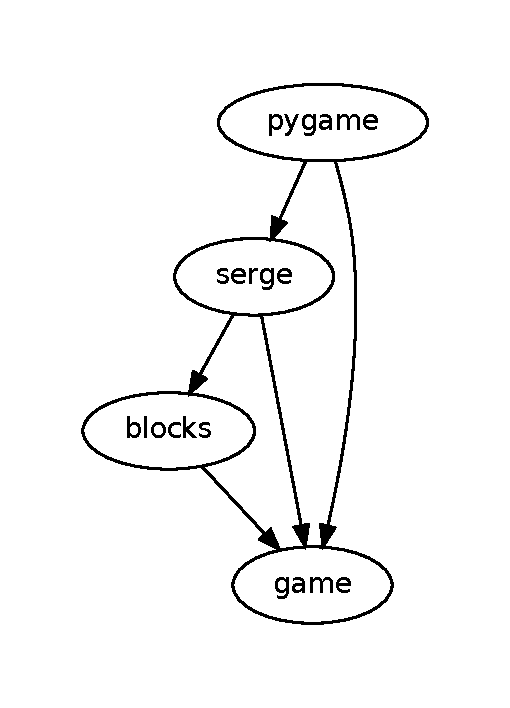
\includegraphics{graphviz-e105d178f146796d84ac12b606890fb9e5d18932.pdf}


\section{Building Blocks}
\label{blocks:building-blocks}\label{blocks::doc}

\subsection{\texttt{achievements} Module}
\label{blocks:module-serge.blocks.achievements}\label{blocks:achievements-module}\index{serge.blocks.achievements (module)}
Represents achievements

Achievements are badges that are assigned to the
player as they play the game. An achievement is
basically a condition that is met. When you meet
the condition you get the badge.
\index{Achievement (class in serge.blocks.achievements)}

\begin{fulllineitems}
\phantomsection\label{blocks:serge.blocks.achievements.Achievement}\pysiglinewithargsret{\strong{class }\code{serge.blocks.achievements.}\bfcode{Achievement}}{\emph{name}, \emph{description}, \emph{badge}, \emph{secret}, \emph{test\_type}, \emph{condition=None}, \emph{condition\_string=None}}{}
Bases: {\hyperref[common:serge.serialize.Serializable]{\code{serge.serialize.Serializable}}}

Represents an achievement
\index{index (serge.blocks.achievements.Achievement attribute)}

\begin{fulllineitems}
\phantomsection\label{blocks:serge.blocks.achievements.Achievement.index}\pysigline{\bfcode{index}\strong{ = 0}}
\end{fulllineitems}

\index{init() (serge.blocks.achievements.Achievement method)}

\begin{fulllineitems}
\phantomsection\label{blocks:serge.blocks.achievements.Achievement.init}\pysiglinewithargsret{\bfcode{init}}{}{}
Initialise the achievement from pickling

\end{fulllineitems}

\index{isMet() (serge.blocks.achievements.Achievement method)}

\begin{fulllineitems}
\phantomsection\label{blocks:serge.blocks.achievements.Achievement.isMet}\pysiglinewithargsret{\bfcode{isMet}}{}{}
Return True if the achievement was met

\end{fulllineitems}

\index{makeReport() (serge.blocks.achievements.Achievement method)}

\begin{fulllineitems}
\phantomsection\label{blocks:serge.blocks.achievements.Achievement.makeReport}\pysiglinewithargsret{\bfcode{makeReport}}{\emph{**kw}}{}
Make a report on this achievement

\end{fulllineitems}

\index{my\_properties (serge.blocks.achievements.Achievement attribute)}

\begin{fulllineitems}
\phantomsection\label{blocks:serge.blocks.achievements.Achievement.my_properties}\pysigline{\bfcode{my\_properties}\strong{ = (`', `', `', 0, `', \textless{}serge.serialize.Obj object at 0x4e61dd0\textgreater{}, `', 0, 0.0)}}
\end{fulllineitems}


\end{fulllineitems}

\index{AchievementBanner (class in serge.blocks.achievements)}

\begin{fulllineitems}
\phantomsection\label{blocks:serge.blocks.achievements.AchievementBanner}\pysiglinewithargsret{\strong{class }\code{serge.blocks.achievements.}\bfcode{AchievementBanner}}{\emph{tag}, \emph{name}, \emph{background\_layer}, \emph{foreground\_layer}, \emph{behaviours}, \emph{theme}}{}
Bases: {\hyperref[actor:serge.actor.MountableActor]{\code{serge.actor.MountableActor}}}

A banner to show an achievment
\index{addedToWorld() (serge.blocks.achievements.AchievementBanner method)}

\begin{fulllineitems}
\phantomsection\label{blocks:serge.blocks.achievements.AchievementBanner.addedToWorld}\pysiglinewithargsret{\bfcode{addedToWorld}}{\emph{world}}{}
Added the banner to the world

\end{fulllineitems}

\index{hideMe() (serge.blocks.achievements.AchievementBanner method)}

\begin{fulllineitems}
\phantomsection\label{blocks:serge.blocks.achievements.AchievementBanner.hideMe}\pysiglinewithargsret{\bfcode{hideMe}}{\emph{world}, \emph{actor}, \emph{interval}}{}
Hide ourself

\end{fulllineitems}

\index{meetAchievement() (serge.blocks.achievements.AchievementBanner method)}

\begin{fulllineitems}
\phantomsection\label{blocks:serge.blocks.achievements.AchievementBanner.meetAchievement}\pysiglinewithargsret{\bfcode{meetAchievement}}{\emph{achievement}, \emph{arg}}{}
An achievement is met

\end{fulllineitems}


\end{fulllineitems}

\index{AchievementManager (class in serge.blocks.achievements)}

\begin{fulllineitems}
\phantomsection\label{blocks:serge.blocks.achievements.AchievementManager}\pysigline{\strong{class }\code{serge.blocks.achievements.}\bfcode{AchievementManager}}
Bases: {\hyperref[common:serge.serialize.Serializable]{\code{serge.serialize.Serializable}}}, {\hyperref[common:serge.common.Loggable]{\code{serge.common.Loggable}}}, {\hyperref[common:serge.common.EventAware]{\code{serge.common.EventAware}}}

Manages all the achievements in the game
\index{getAchievements() (serge.blocks.achievements.AchievementManager method)}

\begin{fulllineitems}
\phantomsection\label{blocks:serge.blocks.achievements.AchievementManager.getAchievements}\pysiglinewithargsret{\bfcode{getAchievements}}{}{}
Return the list of achievements

\end{fulllineitems}

\index{init() (serge.blocks.achievements.AchievementManager method)}

\begin{fulllineitems}
\phantomsection\label{blocks:serge.blocks.achievements.AchievementManager.init}\pysiglinewithargsret{\bfcode{init}}{}{}
Initialise

\end{fulllineitems}

\index{initialiseFromFile() (serge.blocks.achievements.AchievementManager method)}

\begin{fulllineitems}
\phantomsection\label{blocks:serge.blocks.achievements.AchievementManager.initialiseFromFile}\pysiglinewithargsret{\bfcode{initialiseFromFile}}{\emph{filename}}{}
Initialise from the file

\end{fulllineitems}

\index{log (serge.blocks.achievements.AchievementManager attribute)}

\begin{fulllineitems}
\phantomsection\label{blocks:serge.blocks.achievements.AchievementManager.log}\pysigline{\bfcode{log}\strong{ = \textless{}logging.Logger object at 0x4e61fd0\textgreater{}}}
\end{fulllineitems}

\index{makeReport() (serge.blocks.achievements.AchievementManager method)}

\begin{fulllineitems}
\phantomsection\label{blocks:serge.blocks.achievements.AchievementManager.makeReport}\pysiglinewithargsret{\bfcode{makeReport}}{\emph{test\_type}, \emph{**kw}}{}
Make a report on achievements

\end{fulllineitems}

\index{my\_properties (serge.blocks.achievements.AchievementManager attribute)}

\begin{fulllineitems}
\phantomsection\label{blocks:serge.blocks.achievements.AchievementManager.my_properties}\pysigline{\bfcode{my\_properties}\strong{ = (\textless{}serge.serialize.Obj object at 0x4e61e10\textgreater{},)}}
\end{fulllineitems}

\index{registerAchievement() (serge.blocks.achievements.AchievementManager method)}

\begin{fulllineitems}
\phantomsection\label{blocks:serge.blocks.achievements.AchievementManager.registerAchievement}\pysiglinewithargsret{\bfcode{registerAchievement}}{\emph{achievement}}{}
Register an achievement

\end{fulllineitems}

\index{safeRegisterAchievement() (serge.blocks.achievements.AchievementManager method)}

\begin{fulllineitems}
\phantomsection\label{blocks:serge.blocks.achievements.AchievementManager.safeRegisterAchievement}\pysiglinewithargsret{\bfcode{safeRegisterAchievement}}{\emph{achievement}}{}
Register an achievement and do not worry if it is already registered

\end{fulllineitems}

\index{saveAchievements() (serge.blocks.achievements.AchievementManager method)}

\begin{fulllineitems}
\phantomsection\label{blocks:serge.blocks.achievements.AchievementManager.saveAchievements}\pysiglinewithargsret{\bfcode{saveAchievements}}{}{}
Save achievements to a file

\end{fulllineitems}


\end{fulllineitems}

\index{AchievementStatus (class in serge.blocks.achievements)}

\begin{fulllineitems}
\phantomsection\label{blocks:serge.blocks.achievements.AchievementStatus}\pysiglinewithargsret{\strong{class }\code{serge.blocks.achievements.}\bfcode{AchievementStatus}}{\emph{tag}, \emph{name}, \emph{background\_layer}, \emph{foreground\_layer}, \emph{achievement}, \emph{G}}{}
Bases: {\hyperref[actor:serge.actor.MountableActor]{\code{serge.actor.MountableActor}}}

A banner to show an achievment
\index{addedToWorld() (serge.blocks.achievements.AchievementStatus method)}

\begin{fulllineitems}
\phantomsection\label{blocks:serge.blocks.achievements.AchievementStatus.addedToWorld}\pysiglinewithargsret{\bfcode{addedToWorld}}{\emph{world}}{}
Added the banner to the world

\end{fulllineitems}

\index{updateAchievement() (serge.blocks.achievements.AchievementStatus method)}

\begin{fulllineitems}
\phantomsection\label{blocks:serge.blocks.achievements.AchievementStatus.updateAchievement}\pysiglinewithargsret{\bfcode{updateAchievement}}{}{}
Update the achievement view

\end{fulllineitems}


\end{fulllineitems}

\index{AchievementsGrid (class in serge.blocks.achievements)}

\begin{fulllineitems}
\phantomsection\label{blocks:serge.blocks.achievements.AchievementsGrid}\pysiglinewithargsret{\strong{class }\code{serge.blocks.achievements.}\bfcode{AchievementsGrid}}{\emph{G}}{}
Bases: {\hyperref[blocks:serge.blocks.actors.ScreenActor]{\code{serge.blocks.actors.ScreenActor}}}

A grid to show achievements
\index{addedToWorld() (serge.blocks.achievements.AchievementsGrid method)}

\begin{fulllineitems}
\phantomsection\label{blocks:serge.blocks.achievements.AchievementsGrid.addedToWorld}\pysiglinewithargsret{\bfcode{addedToWorld}}{\emph{world}}{}
Added the grid to the world

\end{fulllineitems}

\index{updateAchievements() (serge.blocks.achievements.AchievementsGrid method)}

\begin{fulllineitems}
\phantomsection\label{blocks:serge.blocks.achievements.AchievementsGrid.updateAchievements}\pysiglinewithargsret{\bfcode{updateAchievements}}{\emph{obj}, \emph{arg}}{}
Update all achievements

\end{fulllineitems}


\end{fulllineitems}

\index{BadCondition}

\begin{fulllineitems}
\phantomsection\label{blocks:serge.blocks.achievements.BadCondition}\pysigline{\strong{exception }\code{serge.blocks.achievements.}\bfcode{BadCondition}}
Bases: \code{exceptions.Exception}

The condition was not valid

\end{fulllineitems}

\index{BadReport}

\begin{fulllineitems}
\phantomsection\label{blocks:serge.blocks.achievements.BadReport}\pysigline{\strong{exception }\code{serge.blocks.achievements.}\bfcode{BadReport}}
Bases: \code{exceptions.Exception}

An error occured while evaluating the report

\end{fulllineitems}

\index{BadTestType}

\begin{fulllineitems}
\phantomsection\label{blocks:serge.blocks.achievements.BadTestType}\pysigline{\strong{exception }\code{serge.blocks.achievements.}\bfcode{BadTestType}}
Bases: \code{exceptions.Exception}

The test type was not found

\end{fulllineitems}

\index{DuplicateAchievement}

\begin{fulllineitems}
\phantomsection\label{blocks:serge.blocks.achievements.DuplicateAchievement}\pysigline{\strong{exception }\code{serge.blocks.achievements.}\bfcode{DuplicateAchievement}}
Bases: \code{exceptions.Exception}

An achievement with this name already exists

\end{fulllineitems}

\index{addAchievementsBannerToWorld() (in module serge.blocks.achievements)}

\begin{fulllineitems}
\phantomsection\label{blocks:serge.blocks.achievements.addAchievementsBannerToWorld}\pysiglinewithargsret{\code{serge.blocks.achievements.}\bfcode{addAchievementsBannerToWorld}}{\emph{world}, \emph{front\_layer}, \emph{back\_layer}, \emph{theme}, \emph{manager}}{}
Add a banner for achievements to the world

\end{fulllineitems}

\index{addAchievementsWorld() (in module serge.blocks.achievements)}

\begin{fulllineitems}
\phantomsection\label{blocks:serge.blocks.achievements.addAchievementsWorld}\pysiglinewithargsret{\code{serge.blocks.achievements.}\bfcode{addAchievementsWorld}}{\emph{options}, \emph{theme}}{}
Add a world for the achievements

\end{fulllineitems}

\index{getManager() (in module serge.blocks.achievements)}

\begin{fulllineitems}
\phantomsection\label{blocks:serge.blocks.achievements.getManager}\pysiglinewithargsret{\code{serge.blocks.achievements.}\bfcode{getManager}}{}{}
\end{fulllineitems}

\index{initManager() (in module serge.blocks.achievements)}

\begin{fulllineitems}
\phantomsection\label{blocks:serge.blocks.achievements.initManager}\pysiglinewithargsret{\code{serge.blocks.achievements.}\bfcode{initManager}}{\emph{name}}{}
Initialise and return the manager

\end{fulllineitems}



\subsection{\texttt{actors} Module}
\label{blocks:module-serge.blocks.actors}\label{blocks:actors-module}\index{serge.blocks.actors (module)}
Blocks to help with actors
\index{AnimateThenDieActor (class in serge.blocks.actors)}

\begin{fulllineitems}
\phantomsection\label{blocks:serge.blocks.actors.AnimateThenDieActor}\pysiglinewithargsret{\strong{class }\code{serge.blocks.actors.}\bfcode{AnimateThenDieActor}}{\emph{tag}, \emph{name}, \emph{sprite\_name}, \emph{layer\_name}, \emph{parent=None}}{}
Bases: {\hyperref[actor:serge.actor.Actor]{\code{serge.actor.Actor}}}

An actor that shows its animation and then is removed from the world
\index{addedToWorld() (serge.blocks.actors.AnimateThenDieActor method)}

\begin{fulllineitems}
\phantomsection\label{blocks:serge.blocks.actors.AnimateThenDieActor.addedToWorld}\pysiglinewithargsret{\bfcode{addedToWorld}}{\emph{world}}{}
Added the actor to the world

\end{fulllineitems}

\index{updateActor() (serge.blocks.actors.AnimateThenDieActor method)}

\begin{fulllineitems}
\phantomsection\label{blocks:serge.blocks.actors.AnimateThenDieActor.updateActor}\pysiglinewithargsret{\bfcode{updateActor}}{\emph{interval}, \emph{world}}{}
Update the actor

\end{fulllineitems}


\end{fulllineitems}

\index{FPSDisplay (class in serge.blocks.actors)}

\begin{fulllineitems}
\phantomsection\label{blocks:serge.blocks.actors.FPSDisplay}\pysiglinewithargsret{\strong{class }\code{serge.blocks.actors.}\bfcode{FPSDisplay}}{\emph{x}, \emph{y}, \emph{font\_colour}, \emph{font\_size}, \emph{font\_name='DEFAULT'}}{}
Bases: {\hyperref[blocks:serge.blocks.actors.NumericText]{\code{serge.blocks.actors.NumericText}}}

Displays the current FPS on the screen
\index{addedToWorld() (serge.blocks.actors.FPSDisplay method)}

\begin{fulllineitems}
\phantomsection\label{blocks:serge.blocks.actors.FPSDisplay.addedToWorld}\pysiglinewithargsret{\bfcode{addedToWorld}}{\emph{world}}{}
Added to the world

\end{fulllineitems}

\index{updateActor() (serge.blocks.actors.FPSDisplay method)}

\begin{fulllineitems}
\phantomsection\label{blocks:serge.blocks.actors.FPSDisplay.updateActor}\pysiglinewithargsret{\bfcode{updateActor}}{\emph{interval}, \emph{world}}{}
Update the actor

\end{fulllineitems}


\end{fulllineitems}

\index{FocusManager (class in serge.blocks.actors)}

\begin{fulllineitems}
\phantomsection\label{blocks:serge.blocks.actors.FocusManager}\pysiglinewithargsret{\strong{class }\code{serge.blocks.actors.}\bfcode{FocusManager}}{\emph{tag}, \emph{name}}{}
Bases: {\hyperref[actor:serge.actor.CompositeActor]{\code{serge.actor.CompositeActor}}}

Manages focus between a number of entry widgets
\index{actorEntry() (serge.blocks.actors.FocusManager method)}

\begin{fulllineitems}
\phantomsection\label{blocks:serge.blocks.actors.FocusManager.actorEntry}\pysiglinewithargsret{\bfcode{actorEntry}}{\emph{obj}, \emph{actor}}{}
An entry was accepted

\end{fulllineitems}

\index{actorSelected() (serge.blocks.actors.FocusManager method)}

\begin{fulllineitems}
\phantomsection\label{blocks:serge.blocks.actors.FocusManager.actorSelected}\pysiglinewithargsret{\bfcode{actorSelected}}{\emph{obj}, \emph{actor}}{}
An actor was selected

\end{fulllineitems}

\index{addChild() (serge.blocks.actors.FocusManager method)}

\begin{fulllineitems}
\phantomsection\label{blocks:serge.blocks.actors.FocusManager.addChild}\pysiglinewithargsret{\bfcode{addChild}}{\emph{actor}}{}
Add an actor to the manager

\end{fulllineitems}

\index{addedToWorld() (serge.blocks.actors.FocusManager method)}

\begin{fulllineitems}
\phantomsection\label{blocks:serge.blocks.actors.FocusManager.addedToWorld}\pysiglinewithargsret{\bfcode{addedToWorld}}{\emph{world}}{}
We were added to the world

\end{fulllineitems}

\index{updateActor() (serge.blocks.actors.FocusManager method)}

\begin{fulllineitems}
\phantomsection\label{blocks:serge.blocks.actors.FocusManager.updateActor}\pysiglinewithargsret{\bfcode{updateActor}}{\emph{interval}, \emph{world}}{}
Update the manager

\end{fulllineitems}


\end{fulllineitems}

\index{FormattedText (class in serge.blocks.actors)}

\begin{fulllineitems}
\phantomsection\label{blocks:serge.blocks.actors.FormattedText}\pysiglinewithargsret{\strong{class }\code{serge.blocks.actors.}\bfcode{FormattedText}}{\emph{tag}, \emph{name}, \emph{format}, \emph{colour}, \emph{font\_name='DEFAULT'}, \emph{font\_size=12}, \emph{justify='center'}, \emph{**kw}}{}
Bases: {\hyperref[actor:serge.actor.Actor]{\code{serge.actor.Actor}}}

A text display that can be formatted
\index{getValue() (serge.blocks.actors.FormattedText method)}

\begin{fulllineitems}
\phantomsection\label{blocks:serge.blocks.actors.FormattedText.getValue}\pysiglinewithargsret{\bfcode{getValue}}{\emph{name}}{}
Get the values

\end{fulllineitems}

\index{setValue() (serge.blocks.actors.FormattedText method)}

\begin{fulllineitems}
\phantomsection\label{blocks:serge.blocks.actors.FormattedText.setValue}\pysiglinewithargsret{\bfcode{setValue}}{\emph{name}, \emph{value}}{}
Set the value

\end{fulllineitems}

\index{updateText() (serge.blocks.actors.FormattedText method)}

\begin{fulllineitems}
\phantomsection\label{blocks:serge.blocks.actors.FormattedText.updateText}\pysiglinewithargsret{\bfcode{updateText}}{}{}
Update our text

\end{fulllineitems}


\end{fulllineitems}

\index{InvalidMenu}

\begin{fulllineitems}
\phantomsection\label{blocks:serge.blocks.actors.InvalidMenu}\pysigline{\strong{exception }\code{serge.blocks.actors.}\bfcode{InvalidMenu}}
Bases: \code{exceptions.Exception}

The menu was not valid

\end{fulllineitems}

\index{InvalidMenuItem}

\begin{fulllineitems}
\phantomsection\label{blocks:serge.blocks.actors.InvalidMenuItem}\pysigline{\strong{exception }\code{serge.blocks.actors.}\bfcode{InvalidMenuItem}}
Bases: \code{exceptions.Exception}

The menu item was not understood

\end{fulllineitems}

\index{MuteButton (class in serge.blocks.actors)}

\begin{fulllineitems}
\phantomsection\label{blocks:serge.blocks.actors.MuteButton}\pysiglinewithargsret{\strong{class }\code{serge.blocks.actors.}\bfcode{MuteButton}}{\emph{sprite\_name}, \emph{layer\_name}, \emph{mute\_sound=True}, \emph{mute\_music=True}, \emph{alpha=1.0}}{}
Bases: {\hyperref[actor:serge.actor.Actor]{\code{serge.actor.Actor}}}

A button to mute sound
\index{toggleSound() (serge.blocks.actors.MuteButton method)}

\begin{fulllineitems}
\phantomsection\label{blocks:serge.blocks.actors.MuteButton.toggleSound}\pysiglinewithargsret{\bfcode{toggleSound}}{\emph{obj=None}, \emph{arg=None}}{}
Clicked on the button

\end{fulllineitems}


\end{fulllineitems}

\index{NumericText (class in serge.blocks.actors)}

\begin{fulllineitems}
\phantomsection\label{blocks:serge.blocks.actors.NumericText}\pysiglinewithargsret{\strong{class }\code{serge.blocks.actors.}\bfcode{NumericText}}{\emph{*args}, \emph{**kw}}{}
Bases: {\hyperref[blocks:serge.blocks.actors.FormattedText]{\code{serge.blocks.actors.FormattedText}}}

A helper actor to display some text with a single number in there
\index{updateText() (serge.blocks.actors.NumericText method)}

\begin{fulllineitems}
\phantomsection\label{blocks:serge.blocks.actors.NumericText.updateText}\pysiglinewithargsret{\bfcode{updateText}}{}{}
Update our text

\end{fulllineitems}

\index{value (serge.blocks.actors.NumericText attribute)}

\begin{fulllineitems}
\phantomsection\label{blocks:serge.blocks.actors.NumericText.value}\pysigline{\bfcode{value}}
\end{fulllineitems}


\end{fulllineitems}

\index{RepeatedVisualActor (class in serge.blocks.actors)}

\begin{fulllineitems}
\phantomsection\label{blocks:serge.blocks.actors.RepeatedVisualActor}\pysiglinewithargsret{\strong{class }\code{serge.blocks.actors.}\bfcode{RepeatedVisualActor}}{\emph{tag}, \emph{name=None}, \emph{repeat=5}, \emph{spacing=10}, \emph{orientation='horizontal'}}{}
Bases: {\hyperref[actor:serge.actor.Actor]{\code{serge.actor.Actor}}}

An actor that shows multiple copies of a visual representation

This actor is useful for showing the number of lives or missiles
etc in a game.
\index{getRepeat() (serge.blocks.actors.RepeatedVisualActor method)}

\begin{fulllineitems}
\phantomsection\label{blocks:serge.blocks.actors.RepeatedVisualActor.getRepeat}\pysiglinewithargsret{\bfcode{getRepeat}}{}{}
Return the current repeat

\end{fulllineitems}

\index{increaseRepeat() (serge.blocks.actors.RepeatedVisualActor method)}

\begin{fulllineitems}
\phantomsection\label{blocks:serge.blocks.actors.RepeatedVisualActor.increaseRepeat}\pysiglinewithargsret{\bfcode{increaseRepeat}}{\emph{amount=1}}{}
Increase the repeat by a certain amount

\end{fulllineitems}

\index{reduceRepeat() (serge.blocks.actors.RepeatedVisualActor method)}

\begin{fulllineitems}
\phantomsection\label{blocks:serge.blocks.actors.RepeatedVisualActor.reduceRepeat}\pysiglinewithargsret{\bfcode{reduceRepeat}}{\emph{amount=1}}{}
Reduce the repeat by a certain amount

\end{fulllineitems}

\index{renderTo() (serge.blocks.actors.RepeatedVisualActor method)}

\begin{fulllineitems}
\phantomsection\label{blocks:serge.blocks.actors.RepeatedVisualActor.renderTo}\pysiglinewithargsret{\bfcode{renderTo}}{\emph{renderer}, \emph{interval}}{}
Render ourself to the given renderer

\end{fulllineitems}

\index{resetRepeat() (serge.blocks.actors.RepeatedVisualActor method)}

\begin{fulllineitems}
\phantomsection\label{blocks:serge.blocks.actors.RepeatedVisualActor.resetRepeat}\pysiglinewithargsret{\bfcode{resetRepeat}}{}{}
Reset the repeat to the initial value

\end{fulllineitems}

\index{setRepeat() (serge.blocks.actors.RepeatedVisualActor method)}

\begin{fulllineitems}
\phantomsection\label{blocks:serge.blocks.actors.RepeatedVisualActor.setRepeat}\pysiglinewithargsret{\bfcode{setRepeat}}{\emph{value}}{}
Set the current repeat

\end{fulllineitems}


\end{fulllineitems}

\index{ScreenActor (class in serge.blocks.actors)}

\begin{fulllineitems}
\phantomsection\label{blocks:serge.blocks.actors.ScreenActor}\pysiglinewithargsret{\strong{class }\code{serge.blocks.actors.}\bfcode{ScreenActor}}{\emph{*args}, \emph{**kw}}{}
Bases: {\hyperref[actor:serge.actor.CompositeActor]{\code{serge.actor.CompositeActor}}}

An actor to represent the logic associated with a screen of the game

This actor is useful when encapsulating the logic associated with a specific
screen in the game. The actor has useful properties and methods that
make it easy to manage the logic.
\index{addedToWorld() (serge.blocks.actors.ScreenActor method)}

\begin{fulllineitems}
\phantomsection\label{blocks:serge.blocks.actors.ScreenActor.addedToWorld}\pysiglinewithargsret{\bfcode{addedToWorld}}{\emph{world}}{}
The actor was added to the world

\end{fulllineitems}


\end{fulllineitems}

\index{StringText (class in serge.blocks.actors)}

\begin{fulllineitems}
\phantomsection\label{blocks:serge.blocks.actors.StringText}\pysiglinewithargsret{\strong{class }\code{serge.blocks.actors.}\bfcode{StringText}}{\emph{tag}, \emph{name}, \emph{text}, \emph{format='\%s'}, \emph{colour=(255}, \emph{255}, \emph{255)}, \emph{font\_name='DEFAULT'}, \emph{font\_size=12}, \emph{justify='center'}}{}
Bases: {\hyperref[blocks:serge.blocks.actors.FormattedText]{\code{serge.blocks.actors.FormattedText}}}

A helper actor to display some text with text in there
\index{updateText() (serge.blocks.actors.StringText method)}

\begin{fulllineitems}
\phantomsection\label{blocks:serge.blocks.actors.StringText.updateText}\pysiglinewithargsret{\bfcode{updateText}}{}{}
Update our text

\end{fulllineitems}

\index{value (serge.blocks.actors.StringText attribute)}

\begin{fulllineitems}
\phantomsection\label{blocks:serge.blocks.actors.StringText.value}\pysigline{\bfcode{value}}
\end{fulllineitems}


\end{fulllineitems}

\index{TextEntryWidget (class in serge.blocks.actors)}

\begin{fulllineitems}
\phantomsection\label{blocks:serge.blocks.actors.TextEntryWidget}\pysiglinewithargsret{\strong{class }\code{serge.blocks.actors.}\bfcode{TextEntryWidget}}{\emph{tag}, \emph{name}, \emph{width}, \emph{height}, \emph{colour}, \emph{font\_size}, \emph{font\_name='DEFAULT'}, \emph{justify='center'}, \emph{background\_visual=None}, \emph{background\_layer='background'}, \emph{show\_cursor=False}, \emph{blink\_time=0.5}, \emph{has\_focus=True}}{}
Bases: {\hyperref[actor:serge.actor.MountableActor]{\code{serge.actor.MountableActor}}}

Implements a single line text entry widget

Support letters and numbers. Delete, backspace and left all delete the last
character. Enter triggers an ACCEPT event.
\index{addedToWorld() (serge.blocks.actors.TextEntryWidget method)}

\begin{fulllineitems}
\phantomsection\label{blocks:serge.blocks.actors.TextEntryWidget.addedToWorld}\pysiglinewithargsret{\bfcode{addedToWorld}}{\emph{world}}{}
Added to the world

\end{fulllineitems}

\index{getFocus() (serge.blocks.actors.TextEntryWidget method)}

\begin{fulllineitems}
\phantomsection\label{blocks:serge.blocks.actors.TextEntryWidget.getFocus}\pysiglinewithargsret{\bfcode{getFocus}}{}{}
Get the focus

\end{fulllineitems}

\index{getText() (serge.blocks.actors.TextEntryWidget method)}

\begin{fulllineitems}
\phantomsection\label{blocks:serge.blocks.actors.TextEntryWidget.getText}\pysiglinewithargsret{\bfcode{getText}}{}{}
Return the text value

\end{fulllineitems}

\index{hasFocus() (serge.blocks.actors.TextEntryWidget method)}

\begin{fulllineitems}
\phantomsection\label{blocks:serge.blocks.actors.TextEntryWidget.hasFocus}\pysiglinewithargsret{\bfcode{hasFocus}}{}{}
Return True if we have focus

\end{fulllineitems}

\index{loseFocus() (serge.blocks.actors.TextEntryWidget method)}

\begin{fulllineitems}
\phantomsection\label{blocks:serge.blocks.actors.TextEntryWidget.loseFocus}\pysiglinewithargsret{\bfcode{loseFocus}}{}{}
Lose the focus

\end{fulllineitems}

\index{setLayerName() (serge.blocks.actors.TextEntryWidget method)}

\begin{fulllineitems}
\phantomsection\label{blocks:serge.blocks.actors.TextEntryWidget.setLayerName}\pysiglinewithargsret{\bfcode{setLayerName}}{\emph{layer\_name}}{}
Set the layer name

\end{fulllineitems}

\index{setText() (serge.blocks.actors.TextEntryWidget method)}

\begin{fulllineitems}
\phantomsection\label{blocks:serge.blocks.actors.TextEntryWidget.setText}\pysiglinewithargsret{\bfcode{setText}}{\emph{text}}{}
Set the text value

\end{fulllineitems}

\index{updateActor() (serge.blocks.actors.TextEntryWidget method)}

\begin{fulllineitems}
\phantomsection\label{blocks:serge.blocks.actors.TextEntryWidget.updateActor}\pysiglinewithargsret{\bfcode{updateActor}}{\emph{interval}, \emph{world}}{}
Update the entry widget

\end{fulllineitems}


\end{fulllineitems}

\index{ToggledMenu (class in serge.blocks.actors)}

\begin{fulllineitems}
\phantomsection\label{blocks:serge.blocks.actors.ToggledMenu}\pysiglinewithargsret{\strong{class }\code{serge.blocks.actors.}\bfcode{ToggledMenu}}{\emph{tag}, \emph{name}, \emph{items}, \emph{layout}, \emph{default}, \emph{on\_colour}, \emph{off\_colour}, \emph{width=100}, \emph{height=100}, \emph{callback=None}, \emph{font\_colour=(255}, \emph{255}, \emph{255}, \emph{255)}, \emph{font\_name='DEFAULT'}, \emph{font\_size=12}}{}
Bases: {\hyperref[actor:serge.actor.MountableActor]{\code{serge.actor.MountableActor}}}

Implements a menu of options that can be toggled
\index{getSelection() (serge.blocks.actors.ToggledMenu method)}

\begin{fulllineitems}
\phantomsection\label{blocks:serge.blocks.actors.ToggledMenu.getSelection}\pysiglinewithargsret{\bfcode{getSelection}}{}{}
Return the current selection

\end{fulllineitems}

\index{getSelectionIndex() (serge.blocks.actors.ToggledMenu method)}

\begin{fulllineitems}
\phantomsection\label{blocks:serge.blocks.actors.ToggledMenu.getSelectionIndex}\pysiglinewithargsret{\bfcode{getSelectionIndex}}{}{}
Return the current selection index

\end{fulllineitems}

\index{selectItem() (serge.blocks.actors.ToggledMenu method)}

\begin{fulllineitems}
\phantomsection\label{blocks:serge.blocks.actors.ToggledMenu.selectItem}\pysiglinewithargsret{\bfcode{selectItem}}{\emph{name}}{}
Select an item by name

\end{fulllineitems}

\index{selectItemIndex() (serge.blocks.actors.ToggledMenu method)}

\begin{fulllineitems}
\phantomsection\label{blocks:serge.blocks.actors.ToggledMenu.selectItemIndex}\pysiglinewithargsret{\bfcode{selectItemIndex}}{\emph{index}}{}
Select an item by its index

\end{fulllineitems}


\end{fulllineitems}



\subsection{\texttt{behaviours} Module}
\label{blocks:behaviours-module}\label{blocks:module-serge.blocks.behaviours}\index{serge.blocks.behaviours (module)}
Classes the implement behaviours
\index{AvoidActor (class in serge.blocks.behaviours)}

\begin{fulllineitems}
\phantomsection\label{blocks:serge.blocks.behaviours.AvoidActor}\pysiglinewithargsret{\strong{class }\code{serge.blocks.behaviours.}\bfcode{AvoidActor}}{\emph{actor}, \emph{x\_speed=1}, \emph{y\_speed=1}, \emph{distance=10}}{}
Bases: {\hyperref[blocks:serge.blocks.behaviours.Behaviour]{\code{serge.blocks.behaviours.Behaviour}}}

Move away from an actor until you reach a certain distance

\end{fulllineitems}

\index{AvoidActorsWithTag (class in serge.blocks.behaviours)}

\begin{fulllineitems}
\phantomsection\label{blocks:serge.blocks.behaviours.AvoidActorsWithTag}\pysiglinewithargsret{\strong{class }\code{serge.blocks.behaviours.}\bfcode{AvoidActorsWithTag}}{\emph{tag}, \emph{x\_speed=1}, \emph{y\_speed=1}, \emph{distance=10}}{}
Bases: {\hyperref[blocks:serge.blocks.behaviours.Behaviour]{\code{serge.blocks.behaviours.Behaviour}}}

Move away from multiple actors until you read a certain distance

\end{fulllineitems}

\index{Behaviour (class in serge.blocks.behaviours)}

\begin{fulllineitems}
\phantomsection\label{blocks:serge.blocks.behaviours.Behaviour}\pysigline{\strong{class }\code{serge.blocks.behaviours.}\bfcode{Behaviour}}
Bases: {\hyperref[common:serge.common.Loggable]{\code{serge.common.Loggable}}}

Base class for all behaviours

\end{fulllineitems}

\index{BehaviourAlreadyPaused}

\begin{fulllineitems}
\phantomsection\label{blocks:serge.blocks.behaviours.BehaviourAlreadyPaused}\pysigline{\strong{exception }\code{serge.blocks.behaviours.}\bfcode{BehaviourAlreadyPaused}}
Bases: \code{exceptions.Exception}

The behaviour was already paused

\end{fulllineitems}

\index{BehaviourManager (class in serge.blocks.behaviours)}

\begin{fulllineitems}
\phantomsection\label{blocks:serge.blocks.behaviours.BehaviourManager}\pysiglinewithargsret{\strong{class }\code{serge.blocks.behaviours.}\bfcode{BehaviourManager}}{\emph{*args}, \emph{**kw}}{}
Bases: {\hyperref[actor:serge.actor.Actor]{\code{serge.actor.Actor}}}

Manages the behaviour of multiple actors in a world
\index{assignBehaviour() (serge.blocks.behaviours.BehaviourManager method)}

\begin{fulllineitems}
\phantomsection\label{blocks:serge.blocks.behaviours.BehaviourManager.assignBehaviour}\pysiglinewithargsret{\bfcode{assignBehaviour}}{\emph{actor}, \emph{behaviour}, \emph{name}}{}
Assign a behaviour to an actor

\end{fulllineitems}

\index{hasBehaviour() (serge.blocks.behaviours.BehaviourManager method)}

\begin{fulllineitems}
\phantomsection\label{blocks:serge.blocks.behaviours.BehaviourManager.hasBehaviour}\pysiglinewithargsret{\bfcode{hasBehaviour}}{\emph{record}}{}
Return True if we have a particular behaviour record

\end{fulllineitems}

\index{pauseBehaviours() (serge.blocks.behaviours.BehaviourManager method)}

\begin{fulllineitems}
\phantomsection\label{blocks:serge.blocks.behaviours.BehaviourManager.pauseBehaviours}\pysiglinewithargsret{\bfcode{pauseBehaviours}}{\emph{name}}{}
Pause all behaviours with the name

\end{fulllineitems}

\index{removeBehaviour() (serge.blocks.behaviours.BehaviourManager method)}

\begin{fulllineitems}
\phantomsection\label{blocks:serge.blocks.behaviours.BehaviourManager.removeBehaviour}\pysiglinewithargsret{\bfcode{removeBehaviour}}{\emph{record}}{}
Remove a particular behaviour

\end{fulllineitems}

\index{removeBehaviourByName() (serge.blocks.behaviours.BehaviourManager method)}

\begin{fulllineitems}
\phantomsection\label{blocks:serge.blocks.behaviours.BehaviourManager.removeBehaviourByName}\pysiglinewithargsret{\bfcode{removeBehaviourByName}}{\emph{actor}, \emph{name}}{}
Remove the named behaviour for an actor based on its name

\end{fulllineitems}

\index{removeBehaviours() (serge.blocks.behaviours.BehaviourManager method)}

\begin{fulllineitems}
\phantomsection\label{blocks:serge.blocks.behaviours.BehaviourManager.removeBehaviours}\pysiglinewithargsret{\bfcode{removeBehaviours}}{\emph{behaviours}}{}
Remove a list of behaviours

\end{fulllineitems}

\index{removeBehavioursByName() (serge.blocks.behaviours.BehaviourManager method)}

\begin{fulllineitems}
\phantomsection\label{blocks:serge.blocks.behaviours.BehaviourManager.removeBehavioursByName}\pysiglinewithargsret{\bfcode{removeBehavioursByName}}{\emph{name}}{}
Remove the named behaviour for all actors based on a name

\end{fulllineitems}

\index{restartBehaviours() (serge.blocks.behaviours.BehaviourManager method)}

\begin{fulllineitems}
\phantomsection\label{blocks:serge.blocks.behaviours.BehaviourManager.restartBehaviours}\pysiglinewithargsret{\bfcode{restartBehaviours}}{\emph{name}}{}
Restart all behaviours with the name

\end{fulllineitems}

\index{updateActor() (serge.blocks.behaviours.BehaviourManager method)}

\begin{fulllineitems}
\phantomsection\label{blocks:serge.blocks.behaviours.BehaviourManager.updateActor}\pysiglinewithargsret{\bfcode{updateActor}}{\emph{world}, \emph{interval}}{}
Perform all our behaviours

\end{fulllineitems}


\end{fulllineitems}

\index{BehaviourNotPaused}

\begin{fulllineitems}
\phantomsection\label{blocks:serge.blocks.behaviours.BehaviourNotPaused}\pysigline{\strong{exception }\code{serge.blocks.behaviours.}\bfcode{BehaviourNotPaused}}
Bases: \code{exceptions.Exception}

The behaviour was not paused

\end{fulllineitems}

\index{BehaviourRecord (class in serge.blocks.behaviours)}

\begin{fulllineitems}
\phantomsection\label{blocks:serge.blocks.behaviours.BehaviourRecord}\pysiglinewithargsret{\strong{class }\code{serge.blocks.behaviours.}\bfcode{BehaviourRecord}}{\emph{actor}, \emph{behaviour}, \emph{name}}{}
Bases: \code{object}

Represents a record of a requested behaviour
\index{involvesActor() (serge.blocks.behaviours.BehaviourRecord method)}

\begin{fulllineitems}
\phantomsection\label{blocks:serge.blocks.behaviours.BehaviourRecord.involvesActor}\pysiglinewithargsret{\bfcode{involvesActor}}{\emph{actor}}{}
Return True if the behaviour involves the actor

\end{fulllineitems}

\index{isComplete() (serge.blocks.behaviours.BehaviourRecord method)}

\begin{fulllineitems}
\phantomsection\label{blocks:serge.blocks.behaviours.BehaviourRecord.isComplete}\pysiglinewithargsret{\bfcode{isComplete}}{}{}
Return True if we are complete

\end{fulllineitems}

\index{isRunning() (serge.blocks.behaviours.BehaviourRecord method)}

\begin{fulllineitems}
\phantomsection\label{blocks:serge.blocks.behaviours.BehaviourRecord.isRunning}\pysiglinewithargsret{\bfcode{isRunning}}{}{}
Return True if we are running

\end{fulllineitems}

\index{markComplete() (serge.blocks.behaviours.BehaviourRecord method)}

\begin{fulllineitems}
\phantomsection\label{blocks:serge.blocks.behaviours.BehaviourRecord.markComplete}\pysiglinewithargsret{\bfcode{markComplete}}{}{}
Mark the behaviour as complete

The manage can now remove us and no longer try calling.

\end{fulllineitems}

\index{matches() (serge.blocks.behaviours.BehaviourRecord method)}

\begin{fulllineitems}
\phantomsection\label{blocks:serge.blocks.behaviours.BehaviourRecord.matches}\pysiglinewithargsret{\bfcode{matches}}{\emph{actor}, \emph{name}}{}
Return True if this behaviour matches the actor and name

\end{fulllineitems}

\index{matchesName() (serge.blocks.behaviours.BehaviourRecord method)}

\begin{fulllineitems}
\phantomsection\label{blocks:serge.blocks.behaviours.BehaviourRecord.matchesName}\pysiglinewithargsret{\bfcode{matchesName}}{\emph{name}}{}
Return True if this behaviour matches the name

\end{fulllineitems}

\index{pause() (serge.blocks.behaviours.BehaviourRecord method)}

\begin{fulllineitems}
\phantomsection\label{blocks:serge.blocks.behaviours.BehaviourRecord.pause}\pysiglinewithargsret{\bfcode{pause}}{}{}
Pause the behaviour

\end{fulllineitems}

\index{performBehaviour() (serge.blocks.behaviours.BehaviourRecord method)}

\begin{fulllineitems}
\phantomsection\label{blocks:serge.blocks.behaviours.BehaviourRecord.performBehaviour}\pysiglinewithargsret{\bfcode{performBehaviour}}{\emph{interval}, \emph{world}}{}
Perform the actual behaviour

\end{fulllineitems}

\index{restart() (serge.blocks.behaviours.BehaviourRecord method)}

\begin{fulllineitems}
\phantomsection\label{blocks:serge.blocks.behaviours.BehaviourRecord.restart}\pysiglinewithargsret{\bfcode{restart}}{}{}
Restart the behaviour

\end{fulllineitems}


\end{fulllineitems}

\index{Blink (class in serge.blocks.behaviours)}

\begin{fulllineitems}
\phantomsection\label{blocks:serge.blocks.behaviours.Blink}\pysiglinewithargsret{\strong{class }\code{serge.blocks.behaviours.}\bfcode{Blink}}{\emph{actor}, \emph{time}}{}
Bases: {\hyperref[blocks:serge.blocks.behaviours.Behaviour]{\code{serge.blocks.behaviours.Behaviour}}}

Blink an actor on the screen

\end{fulllineitems}

\index{ConstantVelocity (class in serge.blocks.behaviours)}

\begin{fulllineitems}
\phantomsection\label{blocks:serge.blocks.behaviours.ConstantVelocity}\pysiglinewithargsret{\strong{class }\code{serge.blocks.behaviours.}\bfcode{ConstantVelocity}}{\emph{vx}, \emph{vy}}{}
Bases: {\hyperref[blocks:serge.blocks.behaviours.Behaviour]{\code{serge.blocks.behaviours.Behaviour}}}

Move an actor with a constant velocity

\end{fulllineitems}

\index{Delay (class in serge.blocks.behaviours)}

\begin{fulllineitems}
\phantomsection\label{blocks:serge.blocks.behaviours.Delay}\pysiglinewithargsret{\strong{class }\code{serge.blocks.behaviours.}\bfcode{Delay}}{\emph{interval}}{}
Bases: {\hyperref[blocks:serge.blocks.behaviours.TimedOneshotCallback]{\code{serge.blocks.behaviours.TimedOneshotCallback}}}

A delay - just waits and then completes

Usefor for sequences

\end{fulllineitems}

\index{DuplicateBehaviour}

\begin{fulllineitems}
\phantomsection\label{blocks:serge.blocks.behaviours.DuplicateBehaviour}\pysigline{\strong{exception }\code{serge.blocks.behaviours.}\bfcode{DuplicateBehaviour}}
Bases: \code{exceptions.Exception}

The behaviour was already recorded

\end{fulllineitems}

\index{FlashFor (class in serge.blocks.behaviours)}

\begin{fulllineitems}
\phantomsection\label{blocks:serge.blocks.behaviours.FlashFor}\pysiglinewithargsret{\strong{class }\code{serge.blocks.behaviours.}\bfcode{FlashFor}}{\emph{actor}, \emph{time}}{}
Bases: {\hyperref[blocks:serge.blocks.behaviours.Behaviour]{\code{serge.blocks.behaviours.Behaviour}}}

Flash an actor on the screen

When the actor is flashing the property flashing is True.

\end{fulllineitems}

\index{KeyboardNSEW (class in serge.blocks.behaviours)}

\begin{fulllineitems}
\phantomsection\label{blocks:serge.blocks.behaviours.KeyboardNSEW}\pysiglinewithargsret{\strong{class }\code{serge.blocks.behaviours.}\bfcode{KeyboardNSEW}}{\emph{speed}, \emph{n=273}, \emph{s=274}, \emph{e=275}, \emph{w=276}}{}
Bases: {\hyperref[blocks:serge.blocks.behaviours.Behaviour]{\code{serge.blocks.behaviours.Behaviour}}}

Move an actor in ordinal directions according to the keyboard

Set the n, s, e and w to the keys you want to move the actor. If you
do not want any motion then set that direction to None. Set the speed
to be the amount to move per keypress.

\end{fulllineitems}

\index{KeyboardNSEWToVectorCallback (class in serge.blocks.behaviours)}

\begin{fulllineitems}
\phantomsection\label{blocks:serge.blocks.behaviours.KeyboardNSEWToVectorCallback}\pysiglinewithargsret{\strong{class }\code{serge.blocks.behaviours.}\bfcode{KeyboardNSEWToVectorCallback}}{\emph{method}, \emph{event='key-clicked'}, \emph{speed=1}, \emph{n=273}, \emph{s=274}, \emph{e=275}, \emph{w=276}}{}
Bases: {\hyperref[blocks:serge.blocks.behaviours.Behaviour]{\code{serge.blocks.behaviours.Behaviour}}}

Calls a method with direction vector from ordinal directions according to the keyboard

Set the n, s, e and w to the keys you want to move the actor. If you
do not want any motion then set that direction to None. Set the speed
to be the amount to move per keypress.

This is useful when you want to move an object but you need to do
some preprocessing first. This behaviour will allow you to capture the
keypresses.

\end{fulllineitems}

\index{KeyboardQuit (class in serge.blocks.behaviours)}

\begin{fulllineitems}
\phantomsection\label{blocks:serge.blocks.behaviours.KeyboardQuit}\pysiglinewithargsret{\strong{class }\code{serge.blocks.behaviours.}\bfcode{KeyboardQuit}}{\emph{key=27}}{}
Bases: {\hyperref[blocks:serge.blocks.behaviours.Behaviour]{\code{serge.blocks.behaviours.Behaviour}}}

Quit the game based on a keypress

\end{fulllineitems}

\index{MissingBehaviour}

\begin{fulllineitems}
\phantomsection\label{blocks:serge.blocks.behaviours.MissingBehaviour}\pysigline{\strong{exception }\code{serge.blocks.behaviours.}\bfcode{MissingBehaviour}}
Bases: \code{exceptions.Exception}

Could not locate the behaviour

\end{fulllineitems}

\index{MoveTowardsActor (class in serge.blocks.behaviours)}

\begin{fulllineitems}
\phantomsection\label{blocks:serge.blocks.behaviours.MoveTowardsActor}\pysiglinewithargsret{\strong{class }\code{serge.blocks.behaviours.}\bfcode{MoveTowardsActor}}{\emph{actor}, \emph{x\_speed=1}, \emph{y\_speed=1}}{}
Bases: {\hyperref[blocks:serge.blocks.behaviours.Behaviour]{\code{serge.blocks.behaviours.Behaviour}}}

Move an actor towards another actor

\end{fulllineitems}

\index{MoveTowardsPoint (class in serge.blocks.behaviours)}

\begin{fulllineitems}
\phantomsection\label{blocks:serge.blocks.behaviours.MoveTowardsPoint}\pysiglinewithargsret{\strong{class }\code{serge.blocks.behaviours.}\bfcode{MoveTowardsPoint}}{\emph{point}, \emph{x\_speed=1}, \emph{y\_speed=1}}{}
Bases: {\hyperref[blocks:serge.blocks.behaviours.Behaviour]{\code{serge.blocks.behaviours.Behaviour}}}

Move an actor towards a point

\end{fulllineitems}

\index{MoveWithMouse (class in serge.blocks.behaviours)}

\begin{fulllineitems}
\phantomsection\label{blocks:serge.blocks.behaviours.MoveWithMouse}\pysiglinewithargsret{\strong{class }\code{serge.blocks.behaviours.}\bfcode{MoveWithMouse}}{\emph{actor}}{}
Bases: {\hyperref[blocks:serge.blocks.behaviours.Behaviour]{\code{serge.blocks.behaviours.Behaviour}}}

Move the actor with the mouse

\end{fulllineitems}

\index{OneShotSequence (class in serge.blocks.behaviours)}

\begin{fulllineitems}
\phantomsection\label{blocks:serge.blocks.behaviours.OneShotSequence}\pysiglinewithargsret{\strong{class }\code{serge.blocks.behaviours.}\bfcode{OneShotSequence}}{\emph{sequence}}{}
Bases: {\hyperref[blocks:serge.blocks.behaviours.Behaviour]{\code{serge.blocks.behaviours.Behaviour}}}

A behaviour that calls a sequence of other behaviours

\end{fulllineitems}

\index{Optional (class in serge.blocks.behaviours)}

\begin{fulllineitems}
\phantomsection\label{blocks:serge.blocks.behaviours.Optional}\pysiglinewithargsret{\strong{class }\code{serge.blocks.behaviours.}\bfcode{Optional}}{\emph{behaviour}, \emph{arg}, \emph{selector}}{}
Bases: {\hyperref[blocks:serge.blocks.behaviours.TwoOptions]{\code{serge.blocks.behaviours.TwoOptions}}}

A behaviour that is turned on and off by an option

\end{fulllineitems}

\index{ParallaxMotion (class in serge.blocks.behaviours)}

\begin{fulllineitems}
\phantomsection\label{blocks:serge.blocks.behaviours.ParallaxMotion}\pysiglinewithargsret{\strong{class }\code{serge.blocks.behaviours.}\bfcode{ParallaxMotion}}{\emph{parent}, \emph{(sx}, \emph{sy)}}{}
Bases: {\hyperref[blocks:serge.blocks.behaviours.Behaviour]{\code{serge.blocks.behaviours.Behaviour}}}

Move one object in relation to another
\begin{quote}\begin{description}
\item[{Parameters}] \leavevmode\begin{itemize}
\item {} 
\textbf{parent} -- the object to move relative to

\item {} 
\textbf{sx} -- fraction of x movement relative to parent (0.0 = no parallax, 1.0 = stationary)

\item {} 
\textbf{sy} -- fraction of y movement relative to parent

\end{itemize}

\end{description}\end{quote}

\end{fulllineitems}

\index{RemoveWhenOutOfRange (class in serge.blocks.behaviours)}

\begin{fulllineitems}
\phantomsection\label{blocks:serge.blocks.behaviours.RemoveWhenOutOfRange}\pysiglinewithargsret{\strong{class }\code{serge.blocks.behaviours.}\bfcode{RemoveWhenOutOfRange}}{\emph{x\_range}, \emph{y\_range}}{}
Bases: {\hyperref[blocks:serge.blocks.behaviours.Behaviour]{\code{serge.blocks.behaviours.Behaviour}}}

Remove an actor from the world when it is out of a certain range

\end{fulllineitems}

\index{SnapshotOnKey (class in serge.blocks.behaviours)}

\begin{fulllineitems}
\phantomsection\label{blocks:serge.blocks.behaviours.SnapshotOnKey}\pysiglinewithargsret{\strong{class }\code{serge.blocks.behaviours.}\bfcode{SnapshotOnKey}}{\emph{key=115}, \emph{size=(0}, \emph{0}, \emph{800}, \emph{600)}, \emph{location='`}, \emph{overwrite=True}}{}
Bases: {\hyperref[blocks:serge.blocks.behaviours.Behaviour]{\code{serge.blocks.behaviours.Behaviour}}}

Take a snapshot of the screen when the user presses a key

\end{fulllineitems}

\index{SpringTowardsPoint (class in serge.blocks.behaviours)}

\begin{fulllineitems}
\phantomsection\label{blocks:serge.blocks.behaviours.SpringTowardsPoint}\pysiglinewithargsret{\strong{class }\code{serge.blocks.behaviours.}\bfcode{SpringTowardsPoint}}{\emph{point}, \emph{spring\_constant}, \emph{damping}, \emph{dead\_zone=0.1}}{}
Bases: {\hyperref[blocks:serge.blocks.behaviours.Behaviour]{\code{serge.blocks.behaviours.Behaviour}}}

Move an actor towards a point as if on a spring

\end{fulllineitems}

\index{TimedCallback (class in serge.blocks.behaviours)}

\begin{fulllineitems}
\phantomsection\label{blocks:serge.blocks.behaviours.TimedCallback}\pysiglinewithargsret{\strong{class }\code{serge.blocks.behaviours.}\bfcode{TimedCallback}}{\emph{interval}, \emph{callback}}{}
Bases: {\hyperref[blocks:serge.blocks.behaviours.Behaviour]{\code{serge.blocks.behaviours.Behaviour}}}

A callback that gets called at a certain interval

\end{fulllineitems}

\index{TimedOneshotCallback (class in serge.blocks.behaviours)}

\begin{fulllineitems}
\phantomsection\label{blocks:serge.blocks.behaviours.TimedOneshotCallback}\pysiglinewithargsret{\strong{class }\code{serge.blocks.behaviours.}\bfcode{TimedOneshotCallback}}{\emph{interval}, \emph{callback}}{}
Bases: {\hyperref[blocks:serge.blocks.behaviours.TimedCallback]{\code{serge.blocks.behaviours.TimedCallback}}}

A callback that gets called once and only once at an interval

\end{fulllineitems}

\index{TwoOptions (class in serge.blocks.behaviours)}

\begin{fulllineitems}
\phantomsection\label{blocks:serge.blocks.behaviours.TwoOptions}\pysiglinewithargsret{\strong{class }\code{serge.blocks.behaviours.}\bfcode{TwoOptions}}{\emph{b1}, \emph{b2}, \emph{arg}, \emph{selector}}{}
Bases: {\hyperref[blocks:serge.blocks.behaviours.Behaviour]{\code{serge.blocks.behaviours.Behaviour}}}

A behaviour that chooses between two optional behaviours

\end{fulllineitems}



\subsection{\texttt{conversation} Module}
\label{blocks:module-serge.blocks.conversation}\label{blocks:conversation-module}\index{serge.blocks.conversation (module)}
Represents a conversation

A conversation is a set of nodes with optional branches afterwards.

Each node has some text, either a single line or multiple lines.
\index{BadOption}

\begin{fulllineitems}
\phantomsection\label{blocks:serge.blocks.conversation.BadOption}\pysigline{\strong{exception }\code{serge.blocks.conversation.}\bfcode{BadOption}}
Bases: \code{exceptions.Exception}

The option was not found

\end{fulllineitems}

\index{ConversationManager (class in serge.blocks.conversation)}

\begin{fulllineitems}
\phantomsection\label{blocks:serge.blocks.conversation.ConversationManager}\pysiglinewithargsret{\strong{class }\code{serge.blocks.conversation.}\bfcode{ConversationManager}}{\emph{tree}, \emph{callback=None}, \emph{root=None}, \emph{variables=None}}{}
Bases: {\hyperref[common:serge.common.Loggable]{\code{serge.common.Loggable}}}, {\hyperref[common:serge.common.EventAware]{\code{serge.common.EventAware}}}

Manages a conversation
\index{chooseOption() (serge.blocks.conversation.ConversationManager method)}

\begin{fulllineitems}
\phantomsection\label{blocks:serge.blocks.conversation.ConversationManager.chooseOption}\pysiglinewithargsret{\bfcode{chooseOption}}{\emph{name}}{}
Choose an option named name

\end{fulllineitems}

\index{findNode() (serge.blocks.conversation.ConversationManager method)}

\begin{fulllineitems}
\phantomsection\label{blocks:serge.blocks.conversation.ConversationManager.findNode}\pysiglinewithargsret{\bfcode{findNode}}{\emph{*names}}{}
Return the node with the given name

\end{fulllineitems}

\index{findNodeByID() (serge.blocks.conversation.ConversationManager method)}

\begin{fulllineitems}
\phantomsection\label{blocks:serge.blocks.conversation.ConversationManager.findNodeByID}\pysiglinewithargsret{\bfcode{findNodeByID}}{\emph{ID}}{}
Return the node with the given ID

\end{fulllineitems}

\index{fromXMLFile() (serge.blocks.conversation.ConversationManager class method)}

\begin{fulllineitems}
\phantomsection\label{blocks:serge.blocks.conversation.ConversationManager.fromXMLFile}\pysiglinewithargsret{\strong{classmethod }\bfcode{fromXMLFile}}{\emph{filename}}{}
Load from an XML filename

\end{fulllineitems}

\index{getChild() (serge.blocks.conversation.ConversationManager method)}

\begin{fulllineitems}
\phantomsection\label{blocks:serge.blocks.conversation.ConversationManager.getChild}\pysiglinewithargsret{\bfcode{getChild}}{}{}
Return the first child

\end{fulllineitems}

\index{getChildren() (serge.blocks.conversation.ConversationManager method)}

\begin{fulllineitems}
\phantomsection\label{blocks:serge.blocks.conversation.ConversationManager.getChildren}\pysiglinewithargsret{\bfcode{getChildren}}{}{}
Return the children

\end{fulllineitems}

\index{getLink() (serge.blocks.conversation.ConversationManager method)}

\begin{fulllineitems}
\phantomsection\label{blocks:serge.blocks.conversation.ConversationManager.getLink}\pysiglinewithargsret{\bfcode{getLink}}{}{}
Return a link or None if we don't have one

\end{fulllineitems}

\index{getNewManager() (serge.blocks.conversation.ConversationManager method)}

\begin{fulllineitems}
\phantomsection\label{blocks:serge.blocks.conversation.ConversationManager.getNewManager}\pysiglinewithargsret{\bfcode{getNewManager}}{\emph{parent}}{}
Return a new manager pointing to the parent

\end{fulllineitems}

\index{getNodeVariables() (serge.blocks.conversation.ConversationManager method)}

\begin{fulllineitems}
\phantomsection\label{blocks:serge.blocks.conversation.ConversationManager.getNodeVariables}\pysiglinewithargsret{\bfcode{getNodeVariables}}{\emph{node}}{}
Return the variables for this node

\end{fulllineitems}

\index{getParent() (serge.blocks.conversation.ConversationManager method)}

\begin{fulllineitems}
\phantomsection\label{blocks:serge.blocks.conversation.ConversationManager.getParent}\pysiglinewithargsret{\bfcode{getParent}}{}{}
Return the parent node

\end{fulllineitems}

\index{getText() (serge.blocks.conversation.ConversationManager method)}

\begin{fulllineitems}
\phantomsection\label{blocks:serge.blocks.conversation.ConversationManager.getText}\pysiglinewithargsret{\bfcode{getText}}{}{}
Return the text for this node

\end{fulllineitems}

\index{getVariable() (serge.blocks.conversation.ConversationManager method)}

\begin{fulllineitems}
\phantomsection\label{blocks:serge.blocks.conversation.ConversationManager.getVariable}\pysiglinewithargsret{\bfcode{getVariable}}{\emph{name}}{}
Return the value of a variable

\end{fulllineitems}

\index{moveNext() (serge.blocks.conversation.ConversationManager method)}

\begin{fulllineitems}
\phantomsection\label{blocks:serge.blocks.conversation.ConversationManager.moveNext}\pysiglinewithargsret{\bfcode{moveNext}}{}{}
Move on to the next node

\end{fulllineitems}

\index{parseRichText() (serge.blocks.conversation.ConversationManager method)}

\begin{fulllineitems}
\phantomsection\label{blocks:serge.blocks.conversation.ConversationManager.parseRichText}\pysiglinewithargsret{\bfcode{parseRichText}}{\emph{lines}, \emph{data}}{}
Return the variables and text from a rich text list

\end{fulllineitems}

\index{processNodeVariables() (serge.blocks.conversation.ConversationManager method)}

\begin{fulllineitems}
\phantomsection\label{blocks:serge.blocks.conversation.ConversationManager.processNodeVariables}\pysiglinewithargsret{\bfcode{processNodeVariables}}{\emph{node}}{}
Process variables in the current node

\end{fulllineitems}

\index{restartConversation() (serge.blocks.conversation.ConversationManager method)}

\begin{fulllineitems}
\phantomsection\label{blocks:serge.blocks.conversation.ConversationManager.restartConversation}\pysiglinewithargsret{\bfcode{restartConversation}}{}{}
Try to restart the conversation

\end{fulllineitems}

\index{setCallback() (serge.blocks.conversation.ConversationManager method)}

\begin{fulllineitems}
\phantomsection\label{blocks:serge.blocks.conversation.ConversationManager.setCallback}\pysiglinewithargsret{\bfcode{setCallback}}{\emph{callback}}{}
Set the callback

\end{fulllineitems}


\end{fulllineitems}

\index{InvalidFile}

\begin{fulllineitems}
\phantomsection\label{blocks:serge.blocks.conversation.InvalidFile}\pysigline{\strong{exception }\code{serge.blocks.conversation.}\bfcode{InvalidFile}}
Bases: \code{exceptions.Exception}

The XML file was not valid

\end{fulllineitems}

\index{NodeNotFound}

\begin{fulllineitems}
\phantomsection\label{blocks:serge.blocks.conversation.NodeNotFound}\pysigline{\strong{exception }\code{serge.blocks.conversation.}\bfcode{NodeNotFound}}
Bases: \code{exceptions.Exception}

The node was not found in the tree

\end{fulllineitems}



\subsection{\texttt{directions} Module}
\label{blocks:directions-module}\label{blocks:module-serge.blocks.directions}\index{serge.blocks.directions (module)}
Utilities to do with cardinal directions
\index{getAngleFromCardinal() (in module serge.blocks.directions)}

\begin{fulllineitems}
\phantomsection\label{blocks:serge.blocks.directions.getAngleFromCardinal}\pysiglinewithargsret{\code{serge.blocks.directions.}\bfcode{getAngleFromCardinal}}{\emph{direction}}{}
Return the angle for a cardinal direction

\end{fulllineitems}

\index{getCardinalFromAngle() (in module serge.blocks.directions)}

\begin{fulllineitems}
\phantomsection\label{blocks:serge.blocks.directions.getCardinalFromAngle}\pysiglinewithargsret{\code{serge.blocks.directions.}\bfcode{getCardinalFromAngle}}{\emph{angle}}{}
Return the cardinal for an angle

\end{fulllineitems}

\index{getCardinalFromVector() (in module serge.blocks.directions)}

\begin{fulllineitems}
\phantomsection\label{blocks:serge.blocks.directions.getCardinalFromVector}\pysiglinewithargsret{\code{serge.blocks.directions.}\bfcode{getCardinalFromVector}}{\emph{vector}}{}
Return the cardinal name from the vector

\end{fulllineitems}

\index{getCardinals() (in module serge.blocks.directions)}

\begin{fulllineitems}
\phantomsection\label{blocks:serge.blocks.directions.getCardinals}\pysiglinewithargsret{\code{serge.blocks.directions.}\bfcode{getCardinals}}{}{}
Return the cardinal directions by name

\end{fulllineitems}

\index{getOppositeCardinal() (in module serge.blocks.directions)}

\begin{fulllineitems}
\phantomsection\label{blocks:serge.blocks.directions.getOppositeCardinal}\pysiglinewithargsret{\code{serge.blocks.directions.}\bfcode{getOppositeCardinal}}{\emph{cardinal}}{}
Return the opposite cardinal direction

\end{fulllineitems}

\index{getOppositeVector() (in module serge.blocks.directions)}

\begin{fulllineitems}
\phantomsection\label{blocks:serge.blocks.directions.getOppositeVector}\pysiglinewithargsret{\code{serge.blocks.directions.}\bfcode{getOppositeVector}}{\emph{vector}}{}
Return the opposite vector

\end{fulllineitems}

\index{getVectorFromCardinal() (in module serge.blocks.directions)}

\begin{fulllineitems}
\phantomsection\label{blocks:serge.blocks.directions.getVectorFromCardinal}\pysiglinewithargsret{\code{serge.blocks.directions.}\bfcode{getVectorFromCardinal}}{\emph{direction}}{}
Return the vector for a cardinal direction

\end{fulllineitems}



\subsection{\texttt{dragndrop} Module}
\label{blocks:dragndrop-module}\label{blocks:module-serge.blocks.dragndrop}\index{serge.blocks.dragndrop (module)}
Implements drag and drop behaviour
\index{AlreadyATarget}

\begin{fulllineitems}
\phantomsection\label{blocks:serge.blocks.dragndrop.AlreadyATarget}\pysigline{\strong{exception }\code{serge.blocks.dragndrop.}\bfcode{AlreadyATarget}}
Bases: \code{exceptions.Exception}

The actor is a target already

\end{fulllineitems}

\index{DragController (class in serge.blocks.dragndrop)}

\begin{fulllineitems}
\phantomsection\label{blocks:serge.blocks.dragndrop.DragController}\pysiglinewithargsret{\strong{class }\code{serge.blocks.dragndrop.}\bfcode{DragController}}{\emph{tag='controller'}, \emph{name='controller'}, \emph{start=None}, \emph{stop=None}, \emph{hit=None}, \emph{miss=None}}{}
Bases: {\hyperref[blocks:serge.blocks.actors.ScreenActor]{\code{serge.blocks.actors.ScreenActor}}}

Controls objects which are draggable
\index{addActor() (serge.blocks.dragndrop.DragController method)}

\begin{fulllineitems}
\phantomsection\label{blocks:serge.blocks.dragndrop.DragController.addActor}\pysiglinewithargsret{\bfcode{addActor}}{\emph{actor}, \emph{start=None}, \emph{stop=None}}{}
Add an actor to be controlled and callback to be called when dragging start and stops

\end{fulllineitems}

\index{addDropTarget() (serge.blocks.dragndrop.DragController method)}

\begin{fulllineitems}
\phantomsection\label{blocks:serge.blocks.dragndrop.DragController.addDropTarget}\pysiglinewithargsret{\bfcode{addDropTarget}}{\emph{actor}, \emph{fn=None}}{}
Add a target to drop to

\end{fulllineitems}

\index{checkForDrops() (serge.blocks.dragndrop.DragController method)}

\begin{fulllineitems}
\phantomsection\label{blocks:serge.blocks.dragndrop.DragController.checkForDrops}\pysiglinewithargsret{\bfcode{checkForDrops}}{\emph{actor}}{}
Check to see if we dropped our actor onto a target or not - return False if the drop is not allowed

If we dropped on a target then we can call the callback. If
we didn't drop on a target then we call the miss callback.

The callback can raise DropNotAllowed to cause the drop not to occur

\end{fulllineitems}

\index{clickedActor() (serge.blocks.dragndrop.DragController method)}

\begin{fulllineitems}
\phantomsection\label{blocks:serge.blocks.dragndrop.DragController.clickedActor}\pysiglinewithargsret{\bfcode{clickedActor}}{\emph{obj}, \emph{(actor}, \emph{fn)}}{}
The mouse was released over an actor

\end{fulllineitems}

\index{getDraggedActor() (serge.blocks.dragndrop.DragController method)}

\begin{fulllineitems}
\phantomsection\label{blocks:serge.blocks.dragndrop.DragController.getDraggedActor}\pysiglinewithargsret{\bfcode{getDraggedActor}}{}{}
Return the actor being dragged

\end{fulllineitems}

\index{isDragging() (serge.blocks.dragndrop.DragController method)}

\begin{fulllineitems}
\phantomsection\label{blocks:serge.blocks.dragndrop.DragController.isDragging}\pysiglinewithargsret{\bfcode{isDragging}}{}{}
Return True if we are dragging an object

\end{fulllineitems}

\index{mouseDown() (serge.blocks.dragndrop.DragController method)}

\begin{fulllineitems}
\phantomsection\label{blocks:serge.blocks.dragndrop.DragController.mouseDown}\pysiglinewithargsret{\bfcode{mouseDown}}{\emph{obj}, \emph{(actor}, \emph{fn)}}{}
The mouse was down over an actor

\end{fulllineitems}

\index{removeActor() (serge.blocks.dragndrop.DragController method)}

\begin{fulllineitems}
\phantomsection\label{blocks:serge.blocks.dragndrop.DragController.removeActor}\pysiglinewithargsret{\bfcode{removeActor}}{\emph{actor}}{}
Remove an actor from being controlledd

\end{fulllineitems}

\index{removeDropTarget() (serge.blocks.dragndrop.DragController method)}

\begin{fulllineitems}
\phantomsection\label{blocks:serge.blocks.dragndrop.DragController.removeDropTarget}\pysiglinewithargsret{\bfcode{removeDropTarget}}{\emph{actor}}{}
Remove an actor as a drop target

\end{fulllineitems}

\index{setCallbacks() (serge.blocks.dragndrop.DragController method)}

\begin{fulllineitems}
\phantomsection\label{blocks:serge.blocks.dragndrop.DragController.setCallbacks}\pysiglinewithargsret{\bfcode{setCallbacks}}{\emph{start}, \emph{stop}}{}
Set the callbacks to use when starting and stopping a drag

\end{fulllineitems}

\index{setDropCallbacks() (serge.blocks.dragndrop.DragController method)}

\begin{fulllineitems}
\phantomsection\label{blocks:serge.blocks.dragndrop.DragController.setDropCallbacks}\pysiglinewithargsret{\bfcode{setDropCallbacks}}{\emph{hit}, \emph{miss}}{}
Set the callback to use when dropping on a target

\end{fulllineitems}

\index{updateActor() (serge.blocks.dragndrop.DragController method)}

\begin{fulllineitems}
\phantomsection\label{blocks:serge.blocks.dragndrop.DragController.updateActor}\pysiglinewithargsret{\bfcode{updateActor}}{\emph{interval}, \emph{world}}{}
Update the controller

\end{fulllineitems}


\end{fulllineitems}

\index{DropNotAllowed}

\begin{fulllineitems}
\phantomsection\label{blocks:serge.blocks.dragndrop.DropNotAllowed}\pysigline{\strong{exception }\code{serge.blocks.dragndrop.}\bfcode{DropNotAllowed}}
Bases: \code{exceptions.Exception}

Cannot drop here

\end{fulllineitems}

\index{DuplicateActor}

\begin{fulllineitems}
\phantomsection\label{blocks:serge.blocks.dragndrop.DuplicateActor}\pysigline{\strong{exception }\code{serge.blocks.dragndrop.}\bfcode{DuplicateActor}}
Bases: \code{exceptions.Exception}

The actor is already controlled

\end{fulllineitems}

\index{NotATarget}

\begin{fulllineitems}
\phantomsection\label{blocks:serge.blocks.dragndrop.NotATarget}\pysigline{\strong{exception }\code{serge.blocks.dragndrop.}\bfcode{NotATarget}}
Bases: \code{exceptions.Exception}

The actor is not a target

\end{fulllineitems}

\index{NotDragging}

\begin{fulllineitems}
\phantomsection\label{blocks:serge.blocks.dragndrop.NotDragging}\pysigline{\strong{exception }\code{serge.blocks.dragndrop.}\bfcode{NotDragging}}
Bases: \code{exceptions.Exception}

No actor is being dragged

\end{fulllineitems}



\subsection{\texttt{effects} Module}
\label{blocks:module-serge.blocks.effects}\label{blocks:effects-module}\index{serge.blocks.effects (module)}
Some effects which can alter properties of actors or visuals
\index{AttributeFade (class in serge.blocks.effects)}

\begin{fulllineitems}
\phantomsection\label{blocks:serge.blocks.effects.AttributeFade}\pysiglinewithargsret{\strong{class }\code{serge.blocks.effects.}\bfcode{AttributeFade}}{\emph{obj}, \emph{attribute\_name}, \emph{*args}, \emph{**kw}}{}
Bases: {\hyperref[blocks:serge.blocks.effects.MethodCallFade]{\code{serge.blocks.effects.MethodCallFade}}}

Linearly move an attribute

The attribute changes between a start and an end with a decay.
The decay is the length of time taken to get from the start to the end.

If persistent is set to true then the effect remains in the world to be
re-used. If false then it will be removed when completed.

\end{fulllineitems}

\index{ColourPhaser (class in serge.blocks.effects)}

\begin{fulllineitems}
\phantomsection\label{blocks:serge.blocks.effects.ColourPhaser}\pysiglinewithargsret{\strong{class }\code{serge.blocks.effects.}\bfcode{ColourPhaser}}{\emph{red}, \emph{green}, \emph{blue}, \emph{*args}, \emph{**kw}}{}
Bases: {\hyperref[blocks:serge.blocks.effects.Effect]{\code{serge.blocks.effects.Effect}}}

An effect that causes colours on the whole screen to fade in and out
\index{addedToWorld() (serge.blocks.effects.ColourPhaser method)}

\begin{fulllineitems}
\phantomsection\label{blocks:serge.blocks.effects.ColourPhaser.addedToWorld}\pysiglinewithargsret{\bfcode{addedToWorld}}{\emph{world}}{}
We were added to a wolrd

\end{fulllineitems}

\index{postRender() (serge.blocks.effects.ColourPhaser method)}

\begin{fulllineitems}
\phantomsection\label{blocks:serge.blocks.effects.ColourPhaser.postRender}\pysiglinewithargsret{\bfcode{postRender}}{\emph{obj}, \emph{arg}}{}
Update this effect

\end{fulllineitems}

\index{worldChange() (serge.blocks.effects.ColourPhaser method)}

\begin{fulllineitems}
\phantomsection\label{blocks:serge.blocks.effects.ColourPhaser.worldChange}\pysiglinewithargsret{\bfcode{worldChange}}{\emph{obj}, \emph{active}}{}
The world changed its state

Since we are linked to a renderer event we will be called from all worlds
but we only want to be active when our world is the ative one. We use
the world activation events to toggle our state.

\end{fulllineitems}


\end{fulllineitems}

\index{Effect (class in serge.blocks.effects)}

\begin{fulllineitems}
\phantomsection\label{blocks:serge.blocks.effects.Effect}\pysiglinewithargsret{\strong{class }\code{serge.blocks.effects.}\bfcode{Effect}}{\emph{done=None}, \emph{persistent=False}}{}
Bases: {\hyperref[actor:serge.actor.Actor]{\code{serge.actor.Actor}}}

A generic effect
\index{finish() (serge.blocks.effects.Effect method)}

\begin{fulllineitems}
\phantomsection\label{blocks:serge.blocks.effects.Effect.finish}\pysiglinewithargsret{\bfcode{finish}}{}{}
End the effect

\end{fulllineitems}

\index{pause() (serge.blocks.effects.Effect method)}

\begin{fulllineitems}
\phantomsection\label{blocks:serge.blocks.effects.Effect.pause}\pysiglinewithargsret{\bfcode{pause}}{}{}
Pause the effect

\end{fulllineitems}

\index{restart() (serge.blocks.effects.Effect method)}

\begin{fulllineitems}
\phantomsection\label{blocks:serge.blocks.effects.Effect.restart}\pysiglinewithargsret{\bfcode{restart}}{}{}
Restart the effect

\end{fulllineitems}

\index{unpause() (serge.blocks.effects.Effect method)}

\begin{fulllineitems}
\phantomsection\label{blocks:serge.blocks.effects.Effect.unpause}\pysiglinewithargsret{\bfcode{unpause}}{}{}
Unpause the effect

\end{fulllineitems}


\end{fulllineitems}

\index{InvalidMotion}

\begin{fulllineitems}
\phantomsection\label{blocks:serge.blocks.effects.InvalidMotion}\pysigline{\strong{exception }\code{serge.blocks.effects.}\bfcode{InvalidMotion}}
Bases: \code{exceptions.Exception}

The motion type was not recognized

\end{fulllineitems}

\index{MethodCallFade (class in serge.blocks.effects)}

\begin{fulllineitems}
\phantomsection\label{blocks:serge.blocks.effects.MethodCallFade}\pysiglinewithargsret{\strong{class }\code{serge.blocks.effects.}\bfcode{MethodCallFade}}{\emph{method}, \emph{start}, \emph{end}, \emph{decay}, \emph{persistent=False}, \emph{done=None}, \emph{motion='linear'}}{}
Bases: {\hyperref[blocks:serge.blocks.effects.Effect]{\code{serge.blocks.effects.Effect}}}

Repeated call a method linearly changing the parameter over time

The attribute changes between a start and an end with a decay.
The decay is the length of time taken to get from the start to the end.

If persistent is set to true then the effect remains in the world to be
re-used. If false then it will be removed when completed.

A method can be provided through the done parameter which will be called
when the effect has completed.

The way the variable is moved is dependent on the motion type. This can
be `linear' or `accelerated'.
\index{updateActor() (serge.blocks.effects.MethodCallFade method)}

\begin{fulllineitems}
\phantomsection\label{blocks:serge.blocks.effects.MethodCallFade.updateActor}\pysiglinewithargsret{\bfcode{updateActor}}{\emph{interval}, \emph{world}}{}
Update this effect

\end{fulllineitems}


\end{fulllineitems}

\index{PanActor (class in serge.blocks.effects)}

\begin{fulllineitems}
\phantomsection\label{blocks:serge.blocks.effects.PanActor}\pysiglinewithargsret{\strong{class }\code{serge.blocks.effects.}\bfcode{PanActor}}{\emph{actor}, \emph{speed}, \emph{done=None}, \emph{persistent=False}, \emph{linear=True}}{}
Bases: {\hyperref[blocks:serge.blocks.effects.Effect]{\code{serge.blocks.effects.Effect}}}

Pan an actor across the screen
\index{restart() (serge.blocks.effects.PanActor method)}

\begin{fulllineitems}
\phantomsection\label{blocks:serge.blocks.effects.PanActor.restart}\pysiglinewithargsret{\bfcode{restart}}{}{}
Restart the panning

\end{fulllineitems}

\index{updateActor() (serge.blocks.effects.PanActor method)}

\begin{fulllineitems}
\phantomsection\label{blocks:serge.blocks.effects.PanActor.updateActor}\pysiglinewithargsret{\bfcode{updateActor}}{\emph{interval}, \emph{world}}{}
Update the panning

\end{fulllineitems}


\end{fulllineitems}

\index{Pause (class in serge.blocks.effects)}

\begin{fulllineitems}
\phantomsection\label{blocks:serge.blocks.effects.Pause}\pysiglinewithargsret{\strong{class }\code{serge.blocks.effects.}\bfcode{Pause}}{\emph{time}, \emph{done}, \emph{persistent=False}}{}
Bases: {\hyperref[blocks:serge.blocks.effects.Effect]{\code{serge.blocks.effects.Effect}}}

A simple pause

Used in conjunction with other effects. Calls the done method when
the pause has completed.
\index{updateActor() (serge.blocks.effects.Pause method)}

\begin{fulllineitems}
\phantomsection\label{blocks:serge.blocks.effects.Pause.updateActor}\pysiglinewithargsret{\bfcode{updateActor}}{\emph{interval}, \emph{world}}{}
Update this effect

\end{fulllineitems}


\end{fulllineitems}



\subsection{\texttt{fractals} Module}
\label{blocks:fractals-module}\label{blocks:module-serge.blocks.fractals}\index{serge.blocks.fractals (module)}
Some fractal utilities
\index{fractalLine() (in module serge.blocks.fractals)}

\begin{fulllineitems}
\phantomsection\label{blocks:serge.blocks.fractals.fractalLine}\pysiglinewithargsret{\code{serge.blocks.fractals.}\bfcode{fractalLine}}{\emph{start}, \emph{end}, \emph{number\_steps}, \emph{distance\_per\_step}, \emph{decay}}{}
Return a fractal line, broken into \# steps with each step being a random distance

\end{fulllineitems}

\index{fractalShape() (in module serge.blocks.fractals)}

\begin{fulllineitems}
\phantomsection\label{blocks:serge.blocks.fractals.fractalShape}\pysiglinewithargsret{\code{serge.blocks.fractals.}\bfcode{fractalShape}}{\emph{points}, \emph{number\_steps}, \emph{distance\_per\_step}, \emph{decay}}{}
Return a shape where the straight lines are converted to fractal lines

\end{fulllineitems}



\subsection{\texttt{layout} Module}
\label{blocks:layout-module}\label{blocks:module-serge.blocks.layout}\index{serge.blocks.layout (module)}
Blocks to help with laying out things on the screen
\index{AlreadyInCell}

\begin{fulllineitems}
\phantomsection\label{blocks:serge.blocks.layout.AlreadyInCell}\pysigline{\strong{exception }\code{serge.blocks.layout.}\bfcode{AlreadyInCell}}
Bases: \code{exceptions.Exception}

The actor was already in this cell

\end{fulllineitems}

\index{Bar (class in serge.blocks.layout)}

\begin{fulllineitems}
\phantomsection\label{blocks:serge.blocks.layout.Bar}\pysiglinewithargsret{\strong{class }\code{serge.blocks.layout.}\bfcode{Bar}}{\emph{tag}, \emph{name='`}, \emph{width=None}, \emph{height=None}, \emph{background\_colour=None}, \emph{background\_layer=None}, \emph{background\_sprite=None}}{}
Bases: {\hyperref[blocks:serge.blocks.layout.Container]{\code{serge.blocks.layout.Container}}}

A bar of actors - useful for user interfaces
\index{addActor() (serge.blocks.layout.Bar method)}

\begin{fulllineitems}
\phantomsection\label{blocks:serge.blocks.layout.Bar.addActor}\pysiglinewithargsret{\bfcode{addActor}}{\emph{actor}, \emph{layer\_name=None}}{}
Add an actor to the bar

\end{fulllineitems}

\index{addBlanks() (serge.blocks.layout.Bar method)}

\begin{fulllineitems}
\phantomsection\label{blocks:serge.blocks.layout.Bar.addBlanks}\pysiglinewithargsret{\bfcode{addBlanks}}{\emph{number}}{}
Add blank entries into the bar

\end{fulllineitems}


\end{fulllineitems}

\index{BaseGrid (class in serge.blocks.layout)}

\begin{fulllineitems}
\phantomsection\label{blocks:serge.blocks.layout.BaseGrid}\pysiglinewithargsret{\strong{class }\code{serge.blocks.layout.}\bfcode{BaseGrid}}{\emph{tag}, \emph{name='`}, \emph{size=(1}, \emph{1)}, \emph{width=None}, \emph{height=None}, \emph{background\_colour=None}, \emph{background\_layer=None}}{}
Bases: {\hyperref[blocks:serge.blocks.layout.Container]{\code{serge.blocks.layout.Container}}}

A grid of actors
\index{clearGrid() (serge.blocks.layout.BaseGrid method)}

\begin{fulllineitems}
\phantomsection\label{blocks:serge.blocks.layout.BaseGrid.clearGrid}\pysiglinewithargsret{\bfcode{clearGrid}}{}{}
Clear the entire grid

\end{fulllineitems}

\index{getCoords() (serge.blocks.layout.BaseGrid method)}

\begin{fulllineitems}
\phantomsection\label{blocks:serge.blocks.layout.BaseGrid.getCoords}\pysiglinewithargsret{\bfcode{getCoords}}{\emph{(x}, \emph{y)}}{}
Return the coordinates of a location

\end{fulllineitems}

\index{getLocation() (serge.blocks.layout.BaseGrid method)}

\begin{fulllineitems}
\phantomsection\label{blocks:serge.blocks.layout.BaseGrid.getLocation}\pysiglinewithargsret{\bfcode{getLocation}}{\emph{(x}, \emph{y)}}{}
Return the location in the grid based on coordinates

\end{fulllineitems}

\index{removeActor() (serge.blocks.layout.BaseGrid method)}

\begin{fulllineitems}
\phantomsection\label{blocks:serge.blocks.layout.BaseGrid.removeActor}\pysiglinewithargsret{\bfcode{removeActor}}{\emph{(x}, \emph{y)}}{}
Remove the actor at a certain location

\end{fulllineitems}

\index{removeChildren() (serge.blocks.layout.BaseGrid method)}

\begin{fulllineitems}
\phantomsection\label{blocks:serge.blocks.layout.BaseGrid.removeChildren}\pysiglinewithargsret{\bfcode{removeChildren}}{}{}
Remove all the children

\end{fulllineitems}

\index{setGrid() (serge.blocks.layout.BaseGrid method)}

\begin{fulllineitems}
\phantomsection\label{blocks:serge.blocks.layout.BaseGrid.setGrid}\pysiglinewithargsret{\bfcode{setGrid}}{\emph{(w}, \emph{h)}}{}
Set the size of the grid

This also removes all the current actors from the world. Note that
this can be tricky if you want to re-add some of the actors since
the actors are not actually removed until the next world update
and so you cannot re-add them before this or you will get a duplicate
actor error from the world.

\end{fulllineitems}


\end{fulllineitems}

\index{CellEmpty}

\begin{fulllineitems}
\phantomsection\label{blocks:serge.blocks.layout.CellEmpty}\pysigline{\strong{exception }\code{serge.blocks.layout.}\bfcode{CellEmpty}}
Bases: \code{exceptions.Exception}

The cell being accessed was empty

\end{fulllineitems}

\index{CellOccupied}

\begin{fulllineitems}
\phantomsection\label{blocks:serge.blocks.layout.CellOccupied}\pysigline{\strong{exception }\code{serge.blocks.layout.}\bfcode{CellOccupied}}
Bases: \code{exceptions.Exception}

Tried to put an actor in an occupied cell

\end{fulllineitems}

\index{Container (class in serge.blocks.layout)}

\begin{fulllineitems}
\phantomsection\label{blocks:serge.blocks.layout.Container}\pysiglinewithargsret{\strong{class }\code{serge.blocks.layout.}\bfcode{Container}}{\emph{tag}, \emph{name='`}, \emph{width=None}, \emph{height=None}, \emph{background\_colour=None}, \emph{background\_layer=None}, \emph{background\_sprite=None}}{}
Bases: {\hyperref[actor:serge.actor.MountableActor]{\code{serge.actor.MountableActor}}}

A layout container that contains actors
\index{moveTo() (serge.blocks.layout.Container method)}

\begin{fulllineitems}
\phantomsection\label{blocks:serge.blocks.layout.Container.moveTo}\pysiglinewithargsret{\bfcode{moveTo}}{\emph{x}, \emph{y}, \emph{no\_sync=False}, \emph{override\_lock=True}}{}
Move this actor

\end{fulllineitems}

\index{reflowChildren() (serge.blocks.layout.Container method)}

\begin{fulllineitems}
\phantomsection\label{blocks:serge.blocks.layout.Container.reflowChildren}\pysiglinewithargsret{\bfcode{reflowChildren}}{}{}
Relocate all children

\end{fulllineitems}

\index{setBackgroundColour() (serge.blocks.layout.Container method)}

\begin{fulllineitems}
\phantomsection\label{blocks:serge.blocks.layout.Container.setBackgroundColour}\pysiglinewithargsret{\bfcode{setBackgroundColour}}{\emph{colour}}{}
Sets the background colour

\end{fulllineitems}

\index{setBackgroundSprite() (serge.blocks.layout.Container method)}

\begin{fulllineitems}
\phantomsection\label{blocks:serge.blocks.layout.Container.setBackgroundSprite}\pysiglinewithargsret{\bfcode{setBackgroundSprite}}{\emph{name}}{}
Sets the background sprite

\end{fulllineitems}

\index{setLayerName() (serge.blocks.layout.Container method)}

\begin{fulllineitems}
\phantomsection\label{blocks:serge.blocks.layout.Container.setLayerName}\pysiglinewithargsret{\bfcode{setLayerName}}{\emph{name}}{}
Set the layer name

\end{fulllineitems}


\end{fulllineitems}

\index{Grid (class in serge.blocks.layout)}

\begin{fulllineitems}
\phantomsection\label{blocks:serge.blocks.layout.Grid}\pysiglinewithargsret{\strong{class }\code{serge.blocks.layout.}\bfcode{Grid}}{\emph{tag}, \emph{name='`}, \emph{size=(1}, \emph{1)}, \emph{width=None}, \emph{height=None}, \emph{background\_colour=None}, \emph{background\_layer=None}}{}
Bases: {\hyperref[blocks:serge.blocks.layout.BaseGrid]{\code{serge.blocks.layout.BaseGrid}}}

A grid where a cell can only contain a single actor
\index{addActor() (serge.blocks.layout.Grid method)}

\begin{fulllineitems}
\phantomsection\label{blocks:serge.blocks.layout.Grid.addActor}\pysiglinewithargsret{\bfcode{addActor}}{\emph{(x}, \emph{y)}, \emph{actor}, \emph{layer\_name=None}}{}
Add an actor to the grid

\end{fulllineitems}

\index{autoAddActor() (serge.blocks.layout.Grid method)}

\begin{fulllineitems}
\phantomsection\label{blocks:serge.blocks.layout.Grid.autoAddActor}\pysiglinewithargsret{\bfcode{autoAddActor}}{\emph{actor}}{}
Automatically add an actor to the next cell in the grid

This fills horizontally and then vertically

\end{fulllineitems}

\index{findActorLocation() (serge.blocks.layout.Grid method)}

\begin{fulllineitems}
\phantomsection\label{blocks:serge.blocks.layout.Grid.findActorLocation}\pysiglinewithargsret{\bfcode{findActorLocation}}{\emph{actor}}{}
Find the location of an actor

\end{fulllineitems}

\index{getActorAt() (serge.blocks.layout.Grid method)}

\begin{fulllineitems}
\phantomsection\label{blocks:serge.blocks.layout.Grid.getActorAt}\pysiglinewithargsret{\bfcode{getActorAt}}{\emph{(x}, \emph{y)}}{}
Return the actor at a certain location

\end{fulllineitems}

\index{moveActor() (serge.blocks.layout.Grid method)}

\begin{fulllineitems}
\phantomsection\label{blocks:serge.blocks.layout.Grid.moveActor}\pysiglinewithargsret{\bfcode{moveActor}}{\emph{(x}, \emph{y)}, \emph{actor}}{}
Move an actor from wherever it is to the new location

\end{fulllineitems}


\end{fulllineitems}

\index{HorizontalBar (class in serge.blocks.layout)}

\begin{fulllineitems}
\phantomsection\label{blocks:serge.blocks.layout.HorizontalBar}\pysiglinewithargsret{\strong{class }\code{serge.blocks.layout.}\bfcode{HorizontalBar}}{\emph{tag}, \emph{name='`}, \emph{width=None}, \emph{height=None}, \emph{background\_colour=None}, \emph{background\_layer=None}, \emph{background\_sprite=None}}{}
Bases: {\hyperref[blocks:serge.blocks.layout.Bar]{\code{serge.blocks.layout.Bar}}}

A horizontal bar of actors
\index{getCoords() (serge.blocks.layout.HorizontalBar method)}

\begin{fulllineitems}
\phantomsection\label{blocks:serge.blocks.layout.HorizontalBar.getCoords}\pysiglinewithargsret{\bfcode{getCoords}}{\emph{i}}{}
Return the coordinates of our ith location

\end{fulllineitems}


\end{fulllineitems}

\index{MultiGrid (class in serge.blocks.layout)}

\begin{fulllineitems}
\phantomsection\label{blocks:serge.blocks.layout.MultiGrid}\pysiglinewithargsret{\strong{class }\code{serge.blocks.layout.}\bfcode{MultiGrid}}{\emph{tag}, \emph{name='`}, \emph{size=(1}, \emph{1)}, \emph{width=None}, \emph{height=None}, \emph{background\_colour=None}, \emph{background\_layer=None}}{}
Bases: {\hyperref[blocks:serge.blocks.layout.BaseGrid]{\code{serge.blocks.layout.BaseGrid}}}

A grid where each cell can contain multiple actors
\index{addActor() (serge.blocks.layout.MultiGrid method)}

\begin{fulllineitems}
\phantomsection\label{blocks:serge.blocks.layout.MultiGrid.addActor}\pysiglinewithargsret{\bfcode{addActor}}{\emph{(x}, \emph{y)}, \emph{actor}, \emph{layer\_name=None}}{}
Add an actor to the grid

\end{fulllineitems}

\index{findActorLocation() (serge.blocks.layout.MultiGrid method)}

\begin{fulllineitems}
\phantomsection\label{blocks:serge.blocks.layout.MultiGrid.findActorLocation}\pysiglinewithargsret{\bfcode{findActorLocation}}{\emph{actor}}{}
Find the location of an actor

\end{fulllineitems}

\index{getActorsAt() (serge.blocks.layout.MultiGrid method)}

\begin{fulllineitems}
\phantomsection\label{blocks:serge.blocks.layout.MultiGrid.getActorsAt}\pysiglinewithargsret{\bfcode{getActorsAt}}{\emph{(x}, \emph{y)}}{}
Return the actors at a certain location

\end{fulllineitems}

\index{moveActor() (serge.blocks.layout.MultiGrid method)}

\begin{fulllineitems}
\phantomsection\label{blocks:serge.blocks.layout.MultiGrid.moveActor}\pysiglinewithargsret{\bfcode{moveActor}}{\emph{(x}, \emph{y)}, \emph{actor}}{}
Move an actor from wherever it is to the new location

\end{fulllineitems}

\index{removeActor() (serge.blocks.layout.MultiGrid method)}

\begin{fulllineitems}
\phantomsection\label{blocks:serge.blocks.layout.MultiGrid.removeActor}\pysiglinewithargsret{\bfcode{removeActor}}{\emph{(x}, \emph{y)}, \emph{actor}}{}
Remove the actor at a certain location

\end{fulllineitems}

\index{removeActors() (serge.blocks.layout.MultiGrid method)}

\begin{fulllineitems}
\phantomsection\label{blocks:serge.blocks.layout.MultiGrid.removeActors}\pysiglinewithargsret{\bfcode{removeActors}}{\emph{(x}, \emph{y)}}{}
Remove all the actor from a certain location

\end{fulllineitems}


\end{fulllineitems}

\index{OutOfRange}

\begin{fulllineitems}
\phantomsection\label{blocks:serge.blocks.layout.OutOfRange}\pysigline{\strong{exception }\code{serge.blocks.layout.}\bfcode{OutOfRange}}
Bases: \code{exceptions.Exception}

Tried to find something outside the range of the container

\end{fulllineitems}

\index{UnknownActor}

\begin{fulllineitems}
\phantomsection\label{blocks:serge.blocks.layout.UnknownActor}\pysigline{\strong{exception }\code{serge.blocks.layout.}\bfcode{UnknownActor}}
Bases: \code{exceptions.Exception}

The actor was not found

\end{fulllineitems}

\index{VerticalBar (class in serge.blocks.layout)}

\begin{fulllineitems}
\phantomsection\label{blocks:serge.blocks.layout.VerticalBar}\pysiglinewithargsret{\strong{class }\code{serge.blocks.layout.}\bfcode{VerticalBar}}{\emph{tag}, \emph{name='`}, \emph{width=None}, \emph{height=None}, \emph{background\_colour=None}, \emph{background\_layer=None}, \emph{background\_sprite=None}}{}
Bases: {\hyperref[blocks:serge.blocks.layout.Bar]{\code{serge.blocks.layout.Bar}}}

A vertical bar of actors

\end{fulllineitems}



\subsection{\texttt{scores} Module}
\label{blocks:module-serge.blocks.scores}\label{blocks:scores-module}\index{serge.blocks.scores (module)}
Handling high score type tables
\index{BadCategory}

\begin{fulllineitems}
\phantomsection\label{blocks:serge.blocks.scores.BadCategory}\pysigline{\strong{exception }\code{serge.blocks.scores.}\bfcode{BadCategory}}
Bases: \code{exceptions.Exception}

The category was not found

\end{fulllineitems}

\index{BadData}

\begin{fulllineitems}
\phantomsection\label{blocks:serge.blocks.scores.BadData}\pysigline{\strong{exception }\code{serge.blocks.scores.}\bfcode{BadData}}
Bases: \code{exceptions.Exception}

The data provided for a category was not valid

\end{fulllineitems}

\index{Category (class in serge.blocks.scores)}

\begin{fulllineitems}
\phantomsection\label{blocks:serge.blocks.scores.Category}\pysiglinewithargsret{\strong{class }\code{serge.blocks.scores.}\bfcode{Category}}{\emph{name}, \emph{number=None}, \emph{sort\_columns=None}, \emph{directions=(`ascending'}, \emph{)}}{}
Bases: \code{list}

A category for an individual score table
\index{addScore() (serge.blocks.scores.Category method)}

\begin{fulllineitems}
\phantomsection\label{blocks:serge.blocks.scores.Category.addScore}\pysiglinewithargsret{\bfcode{addScore}}{\emph{name}, \emph{*args}}{}
Add a new score

\end{fulllineitems}

\index{resetCategory() (serge.blocks.scores.Category method)}

\begin{fulllineitems}
\phantomsection\label{blocks:serge.blocks.scores.Category.resetCategory}\pysiglinewithargsret{\bfcode{resetCategory}}{}{}
Reset this category, deleting all the data but maintaining the configuration

\end{fulllineitems}


\end{fulllineitems}

\index{DuplicateCategory}

\begin{fulllineitems}
\phantomsection\label{blocks:serge.blocks.scores.DuplicateCategory}\pysigline{\strong{exception }\code{serge.blocks.scores.}\bfcode{DuplicateCategory}}
Bases: \code{exceptions.Exception}

The category was already added

\end{fulllineitems}

\index{HighScoreTable (class in serge.blocks.scores)}

\begin{fulllineitems}
\phantomsection\label{blocks:serge.blocks.scores.HighScoreTable}\pysigline{\strong{class }\code{serge.blocks.scores.}\bfcode{HighScoreTable}}
Bases: {\hyperref[common:serge.serialize.Serializable]{\code{serge.serialize.Serializable}}}

A high score table

The table can contain scores in a number of categories. Each
category is a table with multiple columns. The table can be
sorted by any one column and can have a limited set of 
values
\index{addCategory() (serge.blocks.scores.HighScoreTable method)}

\begin{fulllineitems}
\phantomsection\label{blocks:serge.blocks.scores.HighScoreTable.addCategory}\pysiglinewithargsret{\bfcode{addCategory}}{\emph{name}, \emph{number=None}, \emph{sort\_columns=None}, \emph{directions=(`ascending'}, \emph{)}}{}
Add a new category

\end{fulllineitems}

\index{addScore() (serge.blocks.scores.HighScoreTable method)}

\begin{fulllineitems}
\phantomsection\label{blocks:serge.blocks.scores.HighScoreTable.addScore}\pysiglinewithargsret{\bfcode{addScore}}{\emph{category\_name}, \emph{name}, \emph{*args}}{}
Add a score to a category

\end{fulllineitems}

\index{getCategory() (serge.blocks.scores.HighScoreTable method)}

\begin{fulllineitems}
\phantomsection\label{blocks:serge.blocks.scores.HighScoreTable.getCategory}\pysiglinewithargsret{\bfcode{getCategory}}{\emph{category\_name}}{}
Return a category

\end{fulllineitems}

\index{my\_properties (serge.blocks.scores.HighScoreTable attribute)}

\begin{fulllineitems}
\phantomsection\label{blocks:serge.blocks.scores.HighScoreTable.my_properties}\pysigline{\bfcode{my\_properties}\strong{ = (\{\},)}}
\end{fulllineitems}

\index{resetCategory() (serge.blocks.scores.HighScoreTable method)}

\begin{fulllineitems}
\phantomsection\label{blocks:serge.blocks.scores.HighScoreTable.resetCategory}\pysiglinewithargsret{\bfcode{resetCategory}}{\emph{category\_name}}{}
Reset the category name

\end{fulllineitems}

\index{resetTable() (serge.blocks.scores.HighScoreTable method)}

\begin{fulllineitems}
\phantomsection\label{blocks:serge.blocks.scores.HighScoreTable.resetTable}\pysiglinewithargsret{\bfcode{resetTable}}{}{}
Clear the entire table

\end{fulllineitems}


\end{fulllineitems}

\index{InvalidSort}

\begin{fulllineitems}
\phantomsection\label{blocks:serge.blocks.scores.InvalidSort}\pysigline{\strong{exception }\code{serge.blocks.scores.}\bfcode{InvalidSort}}
Bases: \code{exceptions.Exception}

The sort direction was invalid

\end{fulllineitems}

\index{InvalidSortColumn}

\begin{fulllineitems}
\phantomsection\label{blocks:serge.blocks.scores.InvalidSortColumn}\pysigline{\strong{exception }\code{serge.blocks.scores.}\bfcode{InvalidSortColumn}}
Bases: \code{exceptions.Exception}

The column specified for sorting was not valid

\end{fulllineitems}



\subsection{\texttt{singletons} Module}
\label{blocks:singletons-module}\label{blocks:module-serge.blocks.singletons}\index{serge.blocks.singletons (module)}
Implement a store for singletons
\index{SingletonStore (class in serge.blocks.singletons)}

\begin{fulllineitems}
\phantomsection\label{blocks:serge.blocks.singletons.SingletonStore}\pysigline{\strong{class }\code{serge.blocks.singletons.}\bfcode{SingletonStore}}
Bases: {\hyperref[common:serge.registry.GeneralStore]{\code{serge.registry.GeneralStore}}}

A store for global objects

\end{fulllineitems}



\subsection{\texttt{themes} Module}
\label{blocks:themes-module}\label{blocks:module-serge.blocks.themes}\index{serge.blocks.themes (module)}
Classes to implement themes

Themes are sets of settings that may affect anything. The idea is that
you may have a number of settings to do with visuals on a world and you
want to control those centrally, potentially also allowing things
to switch during a game.

The themes are managed by a manager.
\index{BadInheritance}

\begin{fulllineitems}
\phantomsection\label{blocks:serge.blocks.themes.BadInheritance}\pysigline{\strong{exception }\code{serge.blocks.themes.}\bfcode{BadInheritance}}
Bases: \code{exceptions.Exception}

A theme subclass was not found

\end{fulllineitems}

\index{BadThemeDefinition}

\begin{fulllineitems}
\phantomsection\label{blocks:serge.blocks.themes.BadThemeDefinition}\pysigline{\strong{exception }\code{serge.blocks.themes.}\bfcode{BadThemeDefinition}}
Bases: \code{exceptions.Exception}

The theme was not of the right format

\end{fulllineitems}

\index{BadThemeFile}

\begin{fulllineitems}
\phantomsection\label{blocks:serge.blocks.themes.BadThemeFile}\pysigline{\strong{exception }\code{serge.blocks.themes.}\bfcode{BadThemeFile}}
Bases: \code{exceptions.Exception}

The specified theme file was not found

\end{fulllineitems}

\index{InvalidFormat}

\begin{fulllineitems}
\phantomsection\label{blocks:serge.blocks.themes.InvalidFormat}\pysigline{\strong{exception }\code{serge.blocks.themes.}\bfcode{InvalidFormat}}
Bases: \code{exceptions.Exception}

The format for the data was invalid

\end{fulllineitems}

\index{Manager (class in serge.blocks.themes)}

\begin{fulllineitems}
\phantomsection\label{blocks:serge.blocks.themes.Manager}\pysigline{\strong{class }\code{serge.blocks.themes.}\bfcode{Manager}}
Bases: \code{object}

Manages a theme
\index{getProperty() (serge.blocks.themes.Manager method)}

\begin{fulllineitems}
\phantomsection\label{blocks:serge.blocks.themes.Manager.getProperty}\pysiglinewithargsret{\bfcode{getProperty}}{\emph{name}, \emph{from\_theme=None}}{}
Return the named property

\end{fulllineitems}

\index{getPropertyWithDefault() (serge.blocks.themes.Manager method)}

\begin{fulllineitems}
\phantomsection\label{blocks:serge.blocks.themes.Manager.getPropertyWithDefault}\pysiglinewithargsret{\bfcode{getPropertyWithDefault}}{\emph{name}, \emph{default}, \emph{from\_theme=None}}{}
Return a property and if it is missing then return the default value

Use this method sparingly. It puts default values in source code
rather than in the theme files.

\end{fulllineitems}

\index{getTheme() (serge.blocks.themes.Manager method)}

\begin{fulllineitems}
\phantomsection\label{blocks:serge.blocks.themes.Manager.getTheme}\pysiglinewithargsret{\bfcode{getTheme}}{\emph{name}}{}
Return a theme object with a default of the given name

\end{fulllineitems}

\index{hasTheme() (serge.blocks.themes.Manager method)}

\begin{fulllineitems}
\phantomsection\label{blocks:serge.blocks.themes.Manager.hasTheme}\pysiglinewithargsret{\bfcode{hasTheme}}{\emph{name}}{}
Return True if we have this theme

\end{fulllineitems}

\index{load() (serge.blocks.themes.Manager method)}

\begin{fulllineitems}
\phantomsection\label{blocks:serge.blocks.themes.Manager.load}\pysiglinewithargsret{\bfcode{load}}{\emph{themes}}{}
Load definitions from a dictionary

\end{fulllineitems}

\index{loadFrom() (serge.blocks.themes.Manager method)}

\begin{fulllineitems}
\phantomsection\label{blocks:serge.blocks.themes.Manager.loadFrom}\pysiglinewithargsret{\bfcode{loadFrom}}{\emph{text}}{}
Load a theme from some text

The theme is a dictionary where each entry is either a theme
or the definition of the schema or the special entry \_\_default\_\_,
which gives the name of the default theme.

If there is an entry then it is a tuple with the name of the
base theme class followed by a dictionary of entries which
overide the base class.

Classes are really just the name of another theme.

\end{fulllineitems}

\index{loadFromFile() (serge.blocks.themes.Manager method)}

\begin{fulllineitems}
\phantomsection\label{blocks:serge.blocks.themes.Manager.loadFromFile}\pysiglinewithargsret{\bfcode{loadFromFile}}{\emph{filename}}{}
Load a theme definition from a file

\end{fulllineitems}

\index{selectTheme() (serge.blocks.themes.Manager method)}

\begin{fulllineitems}
\phantomsection\label{blocks:serge.blocks.themes.Manager.selectTheme}\pysiglinewithargsret{\bfcode{selectTheme}}{\emph{name}}{}
Select the named theme

\end{fulllineitems}

\index{setProperty() (serge.blocks.themes.Manager method)}

\begin{fulllineitems}
\phantomsection\label{blocks:serge.blocks.themes.Manager.setProperty}\pysiglinewithargsret{\bfcode{setProperty}}{\emph{name}, \emph{value}, \emph{from\_theme=None}}{}
Set a property in a theme

\end{fulllineitems}

\index{updateFromString() (serge.blocks.themes.Manager method)}

\begin{fulllineitems}
\phantomsection\label{blocks:serge.blocks.themes.Manager.updateFromString}\pysiglinewithargsret{\bfcode{updateFromString}}{\emph{string}}{}
Update the theme from a string of data
\begin{description}
\item[{Data should be provided as comma separated values like}] \leavevmode
name=''bob'',value=123,etc

\end{description}

\end{fulllineitems}


\end{fulllineitems}

\index{MissingDefault}

\begin{fulllineitems}
\phantomsection\label{blocks:serge.blocks.themes.MissingDefault}\pysigline{\strong{exception }\code{serge.blocks.themes.}\bfcode{MissingDefault}}
Bases: \code{exceptions.Exception}

There was no default theme

\end{fulllineitems}

\index{MissingSchema}

\begin{fulllineitems}
\phantomsection\label{blocks:serge.blocks.themes.MissingSchema}\pysigline{\strong{exception }\code{serge.blocks.themes.}\bfcode{MissingSchema}}
Bases: \code{exceptions.Exception}

There was no schema in the theme definition

\end{fulllineitems}

\index{PropertyNotFound}

\begin{fulllineitems}
\phantomsection\label{blocks:serge.blocks.themes.PropertyNotFound}\pysigline{\strong{exception }\code{serge.blocks.themes.}\bfcode{PropertyNotFound}}
Bases: \code{exceptions.Exception}

Could not find a property

\end{fulllineitems}

\index{ThemeNotFound}

\begin{fulllineitems}
\phantomsection\label{blocks:serge.blocks.themes.ThemeNotFound}\pysigline{\strong{exception }\code{serge.blocks.themes.}\bfcode{ThemeNotFound}}
Bases: \code{exceptions.Exception}

The named scheme was not found

\end{fulllineitems}



\subsection{\texttt{tiled} Module}
\label{blocks:module-serge.blocks.tiled}\label{blocks:tiled-module}\index{serge.blocks.tiled (module)}
Implements an interface to Tiled files
\index{BadLayer}

\begin{fulllineitems}
\phantomsection\label{blocks:serge.blocks.tiled.BadLayer}\pysigline{\strong{exception }\code{serge.blocks.tiled.}\bfcode{BadLayer}}
Bases: \code{exceptions.Exception}

The layer specification was invalid

\end{fulllineitems}

\index{BadTiledFile}

\begin{fulllineitems}
\phantomsection\label{blocks:serge.blocks.tiled.BadTiledFile}\pysigline{\strong{exception }\code{serge.blocks.tiled.}\bfcode{BadTiledFile}}
Bases: \code{exceptions.Exception}

The tiled file could not be found

\end{fulllineitems}

\index{Layer (class in serge.blocks.tiled)}

\begin{fulllineitems}
\phantomsection\label{blocks:serge.blocks.tiled.Layer}\pysiglinewithargsret{\strong{class }\code{serge.blocks.tiled.}\bfcode{Layer}}{\emph{tiled}, \emph{name}, \emph{layer\_type}, \emph{width=None}, \emph{height=None}, \emph{tiles=None}, \emph{properties=None}}{}
Bases: {\hyperref[common:serge.common.Loggable]{\code{serge.common.Loggable}}}

A layer in a tilemap
\index{addObject() (serge.blocks.tiled.Layer method)}

\begin{fulllineitems}
\phantomsection\label{blocks:serge.blocks.tiled.Layer.addObject}\pysiglinewithargsret{\bfcode{addObject}}{\emph{obj}}{}
Add an object

\end{fulllineitems}

\index{getLocationsWithTile() (serge.blocks.tiled.Layer method)}

\begin{fulllineitems}
\phantomsection\label{blocks:serge.blocks.tiled.Layer.getLocationsWithTile}\pysiglinewithargsret{\bfcode{getLocationsWithTile}}{}{}
Return all tile locations with a tile

\end{fulllineitems}

\index{getLocationsWithoutTile() (serge.blocks.tiled.Layer method)}

\begin{fulllineitems}
\phantomsection\label{blocks:serge.blocks.tiled.Layer.getLocationsWithoutTile}\pysiglinewithargsret{\bfcode{getLocationsWithoutTile}}{}{}
Return all tile locations without a tile

\end{fulllineitems}

\index{getObject() (serge.blocks.tiled.Layer method)}

\begin{fulllineitems}
\phantomsection\label{blocks:serge.blocks.tiled.Layer.getObject}\pysiglinewithargsret{\bfcode{getObject}}{\emph{name}}{}
Return the named object

\end{fulllineitems}

\index{getObjects() (serge.blocks.tiled.Layer method)}

\begin{fulllineitems}
\phantomsection\label{blocks:serge.blocks.tiled.Layer.getObjects}\pysiglinewithargsret{\bfcode{getObjects}}{}{}
Return all the objects

\end{fulllineitems}

\index{getSize() (serge.blocks.tiled.Layer method)}

\begin{fulllineitems}
\phantomsection\label{blocks:serge.blocks.tiled.Layer.getSize}\pysiglinewithargsret{\bfcode{getSize}}{}{}
Return the size of the layer

\end{fulllineitems}

\index{getSpriteFor() (serge.blocks.tiled.Layer method)}

\begin{fulllineitems}
\phantomsection\label{blocks:serge.blocks.tiled.Layer.getSpriteFor}\pysiglinewithargsret{\bfcode{getSpriteFor}}{\emph{(x}, \emph{y)}}{}
Return the sprite for a certain location

\end{fulllineitems}

\index{iterCellLocations() (serge.blocks.tiled.Layer method)}

\begin{fulllineitems}
\phantomsection\label{blocks:serge.blocks.tiled.Layer.iterCellLocations}\pysiglinewithargsret{\bfcode{iterCellLocations}}{}{}
Return an interation of the cell locations

\end{fulllineitems}


\end{fulllineitems}

\index{NotFound}

\begin{fulllineitems}
\phantomsection\label{blocks:serge.blocks.tiled.NotFound}\pysigline{\strong{exception }\code{serge.blocks.tiled.}\bfcode{NotFound}}
Bases: \code{exceptions.Exception}

The object was not found

\end{fulllineitems}

\index{TileMap (class in serge.blocks.tiled)}

\begin{fulllineitems}
\phantomsection\label{blocks:serge.blocks.tiled.TileMap}\pysigline{\strong{class }\code{serge.blocks.tiled.}\bfcode{TileMap}}
Bases: {\hyperref[common:serge.common.Loggable]{\code{serge.common.Loggable}}}

A representation of a 2d map of tiles
\index{addLayer() (serge.blocks.tiled.TileMap method)}

\begin{fulllineitems}
\phantomsection\label{blocks:serge.blocks.tiled.TileMap.addLayer}\pysiglinewithargsret{\bfcode{addLayer}}{\emph{layer}}{}
Add a layer

\end{fulllineitems}

\index{addLayerTypes() (serge.blocks.tiled.TileMap class method)}

\begin{fulllineitems}
\phantomsection\label{blocks:serge.blocks.tiled.TileMap.addLayerTypes}\pysiglinewithargsret{\strong{classmethod }\bfcode{addLayerTypes}}{\emph{layer\_types}}{}
Add more layer types

\end{fulllineitems}

\index{getLayer() (serge.blocks.tiled.TileMap method)}

\begin{fulllineitems}
\phantomsection\label{blocks:serge.blocks.tiled.TileMap.getLayer}\pysiglinewithargsret{\bfcode{getLayer}}{\emph{name}}{}
return the tile with a certain name

\end{fulllineitems}

\index{getLayerByType() (serge.blocks.tiled.TileMap method)}

\begin{fulllineitems}
\phantomsection\label{blocks:serge.blocks.tiled.TileMap.getLayerByType}\pysiglinewithargsret{\bfcode{getLayerByType}}{\emph{type\_name}}{}
Return the layer with a given type

\end{fulllineitems}

\index{getLayers() (serge.blocks.tiled.TileMap method)}

\begin{fulllineitems}
\phantomsection\label{blocks:serge.blocks.tiled.TileMap.getLayers}\pysiglinewithargsret{\bfcode{getLayers}}{}{}
Return the layers of tiles

\end{fulllineitems}

\index{getLayersByType() (serge.blocks.tiled.TileMap method)}

\begin{fulllineitems}
\phantomsection\label{blocks:serge.blocks.tiled.TileMap.getLayersByType}\pysiglinewithargsret{\bfcode{getLayersByType}}{\emph{type\_name}}{}
Return the layer with a given type

\end{fulllineitems}

\index{getLayersForTile() (serge.blocks.tiled.TileMap method)}

\begin{fulllineitems}
\phantomsection\label{blocks:serge.blocks.tiled.TileMap.getLayersForTile}\pysiglinewithargsret{\bfcode{getLayersForTile}}{\emph{(x}, \emph{y)}, \emph{excluding=None}}{}
Return a list of the layers that the tile at x, y is set on

\end{fulllineitems}

\index{getPropertiesFrom() (serge.blocks.tiled.TileMap method)}

\begin{fulllineitems}
\phantomsection\label{blocks:serge.blocks.tiled.TileMap.getPropertiesFrom}\pysiglinewithargsret{\bfcode{getPropertiesFrom}}{\emph{nodes}}{}
Return a property disction from the node

\end{fulllineitems}

\index{getPropertyBagArray() (serge.blocks.tiled.TileMap method)}

\begin{fulllineitems}
\phantomsection\label{blocks:serge.blocks.tiled.TileMap.getPropertyBagArray}\pysiglinewithargsret{\bfcode{getPropertyBagArray}}{\emph{sprite\_layers}, \emph{boolean\_layers}, \emph{property\_layers}, \emph{prototype=None}, \emph{optional\_layers=None}}{}
Return an array of property bags for the tile array
\begin{description}
\item[{You pass a series of lists of layer types, which are treated like:}] \leavevmode
sprite\_layers = tile based layers to treat as identifying sprites
boolean\_layers = tile layers where if a tile is set (to anything) then a boolean flag is True
property\_layers = tile layers where if a tile is set then the item recieves all the properties of the layer

\end{description}

\end{fulllineitems}

\index{getSize() (serge.blocks.tiled.TileMap method)}

\begin{fulllineitems}
\phantomsection\label{blocks:serge.blocks.tiled.TileMap.getSize}\pysiglinewithargsret{\bfcode{getSize}}{}{}
Return the size of the map using the first layer as a guide

\end{fulllineitems}

\index{getSpriteName() (serge.blocks.tiled.TileMap method)}

\begin{fulllineitems}
\phantomsection\label{blocks:serge.blocks.tiled.TileMap.getSpriteName}\pysiglinewithargsret{\bfcode{getSpriteName}}{\emph{idx}}{}
Return the sprite name for an index

\end{fulllineitems}

\index{getTypeFrom() (serge.blocks.tiled.TileMap method)}

\begin{fulllineitems}
\phantomsection\label{blocks:serge.blocks.tiled.TileMap.getTypeFrom}\pysiglinewithargsret{\bfcode{getTypeFrom}}{\emph{name}, \emph{properties}}{}
Return the layer type, checking validity which we do it

\end{fulllineitems}

\index{resetLayerTypes() (serge.blocks.tiled.TileMap class method)}

\begin{fulllineitems}
\phantomsection\label{blocks:serge.blocks.tiled.TileMap.resetLayerTypes}\pysiglinewithargsret{\strong{classmethod }\bfcode{resetLayerTypes}}{}{}
Reset the layer types to default

\end{fulllineitems}


\end{fulllineitems}

\index{TileObject (class in serge.blocks.tiled)}

\begin{fulllineitems}
\phantomsection\label{blocks:serge.blocks.tiled.TileObject}\pysiglinewithargsret{\strong{class }\code{serge.blocks.tiled.}\bfcode{TileObject}}{\emph{name}, \emph{object\_type}, \emph{x}, \emph{y}, \emph{width}, \emph{height}, \emph{properties}, \emph{sprite\_name=None}}{}
Bases: {\hyperref[common:serge.common.Loggable]{\code{serge.common.Loggable}}}

A tile

\end{fulllineitems}

\index{Tiled (class in serge.blocks.tiled)}

\begin{fulllineitems}
\phantomsection\label{blocks:serge.blocks.tiled.Tiled}\pysiglinewithargsret{\strong{class }\code{serge.blocks.tiled.}\bfcode{Tiled}}{\emph{filename}}{}
Bases: {\hyperref[blocks:serge.blocks.tiled.TileMap]{\code{serge.blocks.tiled.TileMap}}}

An interface to tiled files
\index{getObjectLayers() (serge.blocks.tiled.Tiled method)}

\begin{fulllineitems}
\phantomsection\label{blocks:serge.blocks.tiled.Tiled.getObjectLayers}\pysiglinewithargsret{\bfcode{getObjectLayers}}{}{}
Return the object layers

\end{fulllineitems}

\index{layer\_types (serge.blocks.tiled.Tiled attribute)}

\begin{fulllineitems}
\phantomsection\label{blocks:serge.blocks.tiled.Tiled.layer_types}\pysigline{\bfcode{layer\_types}\strong{ = {[}'visual', `adhoc-visual', `movement', `visibility', `object', `resistance'{]}}}
\end{fulllineitems}


\end{fulllineitems}



\subsection{\texttt{utils} Module}
\label{blocks:module-serge.blocks.utils}\label{blocks:utils-module}\index{serge.blocks.utils (module)}
Some utilities that speed up common operations
\index{MovieRecorder (class in serge.blocks.utils)}

\begin{fulllineitems}
\phantomsection\label{blocks:serge.blocks.utils.MovieRecorder}\pysiglinewithargsret{\strong{class }\code{serge.blocks.utils.}\bfcode{MovieRecorder}}{\emph{path}, \emph{make\_movie=False}, \emph{rate=1}, \emph{in\_memory=False}}{}
Bases: \code{object}

Will record a movie of the game
\index{clearFrames() (serge.blocks.utils.MovieRecorder method)}

\begin{fulllineitems}
\phantomsection\label{blocks:serge.blocks.utils.MovieRecorder.clearFrames}\pysiglinewithargsret{\bfcode{clearFrames}}{}{}
Clear all current frames

\end{fulllineitems}

\index{makeFrame() (serge.blocks.utils.MovieRecorder method)}

\begin{fulllineitems}
\phantomsection\label{blocks:serge.blocks.utils.MovieRecorder.makeFrame}\pysiglinewithargsret{\bfcode{makeFrame}}{\emph{obj}, \emph{arg}}{}
Make a frame

\end{fulllineitems}

\index{makeMovie() (serge.blocks.utils.MovieRecorder method)}

\begin{fulllineitems}
\phantomsection\label{blocks:serge.blocks.utils.MovieRecorder.makeMovie}\pysiglinewithargsret{\bfcode{makeMovie}}{\emph{obj}, \emph{arg}}{}
Convert the frames to movie

\end{fulllineitems}


\end{fulllineitems}

\index{RecordDesktop (class in serge.blocks.utils)}

\begin{fulllineitems}
\phantomsection\label{blocks:serge.blocks.utils.RecordDesktop}\pysiglinewithargsret{\strong{class }\code{serge.blocks.utils.}\bfcode{RecordDesktop}}{\emph{filename}}{}
Bases: {\hyperref[common:serge.common.Loggable]{\code{serge.common.Loggable}}}

Use record my desktop to record the action
\index{stop() (serge.blocks.utils.RecordDesktop method)}

\begin{fulllineitems}
\phantomsection\label{blocks:serge.blocks.utils.RecordDesktop.stop}\pysiglinewithargsret{\bfcode{stop}}{\emph{obj}, \emph{arg}}{}
Stop the recording

\end{fulllineitems}


\end{fulllineitems}

\index{addActorToWorld() (in module serge.blocks.utils)}

\begin{fulllineitems}
\phantomsection\label{blocks:serge.blocks.utils.addActorToWorld}\pysiglinewithargsret{\code{serge.blocks.utils.}\bfcode{addActorToWorld}}{\emph{world}, \emph{actor}, \emph{sprite\_name=None}, \emph{layer\_name=None}, \emph{center\_position=None}, \emph{physics=None}, \emph{origin=None}}{}
Create a new actor in the world

If the center position is not specified then it is placed at the center of the screen.

\end{fulllineitems}

\index{addMuteButtonToWorlds() (in module serge.blocks.utils)}

\begin{fulllineitems}
\phantomsection\label{blocks:serge.blocks.utils.addMuteButtonToWorlds}\pysiglinewithargsret{\code{serge.blocks.utils.}\bfcode{addMuteButtonToWorlds}}{\emph{button}, \emph{center\_position}, \emph{world\_names=None}}{}
Add a particular mute button to various worlds

If worlds is not specified then add to all the worlds currently in the engine.

\end{fulllineitems}

\index{addSpriteActorToWorld() (in module serge.blocks.utils)}

\begin{fulllineitems}
\phantomsection\label{blocks:serge.blocks.utils.addSpriteActorToWorld}\pysiglinewithargsret{\code{serge.blocks.utils.}\bfcode{addSpriteActorToWorld}}{\emph{world}, \emph{tag}, \emph{name}, \emph{sprite\_name}, \emph{layer\_name}, \emph{center\_position=None}, \emph{physics=None}}{}
Create a new actor in the world and set the visual to be the named sprite

If the center position is not specified then it is placed at the center of the screen.

\end{fulllineitems}

\index{addTextItemsToWorld() (in module serge.blocks.utils)}

\begin{fulllineitems}
\phantomsection\label{blocks:serge.blocks.utils.addTextItemsToWorld}\pysiglinewithargsret{\code{serge.blocks.utils.}\bfcode{addTextItemsToWorld}}{\emph{world}, \emph{items}, \emph{theme}, \emph{layer\_name}}{}
Add multiple text items to the world

\end{fulllineitems}

\index{addTextToWorld() (in module serge.blocks.utils)}

\begin{fulllineitems}
\phantomsection\label{blocks:serge.blocks.utils.addTextToWorld}\pysiglinewithargsret{\code{serge.blocks.utils.}\bfcode{addTextToWorld}}{\emph{world}, \emph{text}, \emph{name}, \emph{theme}, \emph{layer\_name}}{}
Add some text to the world

\end{fulllineitems}

\index{addVisualActorToWorld() (in module serge.blocks.utils)}

\begin{fulllineitems}
\phantomsection\label{blocks:serge.blocks.utils.addVisualActorToWorld}\pysiglinewithargsret{\code{serge.blocks.utils.}\bfcode{addVisualActorToWorld}}{\emph{world}, \emph{tag}, \emph{name}, \emph{visual}, \emph{layer\_name}, \emph{center\_position=None}, \emph{physics=None}}{}
Create a new actor in the world and set the visual

If the center position is not specified then it is placed at the center of the screen.

\end{fulllineitems}

\index{backToPreviousWorld() (in module serge.blocks.utils)}

\begin{fulllineitems}
\phantomsection\label{blocks:serge.blocks.utils.backToPreviousWorld}\pysiglinewithargsret{\code{serge.blocks.utils.}\bfcode{backToPreviousWorld}}{\emph{sound=None}}{}
Return an event callback to switch back to the previous world

\end{fulllineitems}

\index{checkNetworkXVersion() (in module serge.blocks.utils)}

\begin{fulllineitems}
\phantomsection\label{blocks:serge.blocks.utils.checkNetworkXVersion}\pysiglinewithargsret{\code{serge.blocks.utils.}\bfcode{checkNetworkXVersion}}{\emph{need\_version}}{}
Check a suitable version of NetworkX is installed

\end{fulllineitems}

\index{checkPythonVersion() (in module serge.blocks.utils)}

\begin{fulllineitems}
\phantomsection\label{blocks:serge.blocks.utils.checkPythonVersion}\pysiglinewithargsret{\code{serge.blocks.utils.}\bfcode{checkPythonVersion}}{}{}
Check a suitable Python version is installed

\end{fulllineitems}

\index{createLayers() (in module serge.blocks.utils)}

\begin{fulllineitems}
\phantomsection\label{blocks:serge.blocks.utils.createLayers}\pysiglinewithargsret{\code{serge.blocks.utils.}\bfcode{createLayers}}{\emph{engine}, \emph{layers}, \emph{cls}}{}
Create a number of layers in the engine using the given class of layer

\end{fulllineitems}

\index{createLayersForEngine() (in module serge.blocks.utils)}

\begin{fulllineitems}
\phantomsection\label{blocks:serge.blocks.utils.createLayersForEngine}\pysiglinewithargsret{\code{serge.blocks.utils.}\bfcode{createLayersForEngine}}{\emph{engine}, \emph{layers}}{}
Add a number of layers to the engine

The layers parameter is a list of layer names. The layers are added to
the renderer of the engine as successive layers in order.

\end{fulllineitems}

\index{createVirtualLayersForEngine() (in module serge.blocks.utils)}

\begin{fulllineitems}
\phantomsection\label{blocks:serge.blocks.utils.createVirtualLayersForEngine}\pysiglinewithargsret{\code{serge.blocks.utils.}\bfcode{createVirtualLayersForEngine}}{\emph{engine}, \emph{layers}}{}
Add a number of virtual layers to the engine

The layers parameter is a list of layer names. The layers are added to
the renderer of the engine as successive layers in order.

The layers are created as virtual, meaning that this will render
quicker than the real layers version, although compositing
will not be possible.

\end{fulllineitems}

\index{createWorldsForEngine() (in module serge.blocks.utils)}

\begin{fulllineitems}
\phantomsection\label{blocks:serge.blocks.utils.createWorldsForEngine}\pysiglinewithargsret{\code{serge.blocks.utils.}\bfcode{createWorldsForEngine}}{\emph{engine}, \emph{worlds}}{}
Add a numer of worlds to the engine

The words parameter is a list of names of the worlds to create.
Each world is created with a single active zone which is quite
large.

\end{fulllineitems}

\index{debugMethod() (in module serge.blocks.utils)}

\begin{fulllineitems}
\phantomsection\label{blocks:serge.blocks.utils.debugMethod}\pysiglinewithargsret{\code{serge.blocks.utils.}\bfcode{debugMethod}}{\emph{obj}, \emph{method\_name}, \emph{logger=None}, \emph{fmt='`}}{}
Create a debug logged method

\end{fulllineitems}

\index{getGamePath() (in module serge.blocks.utils)}

\begin{fulllineitems}
\phantomsection\label{blocks:serge.blocks.utils.getGamePath}\pysiglinewithargsret{\code{serge.blocks.utils.}\bfcode{getGamePath}}{\emph{*parts}}{}
Return a path based on the main game folder

\end{fulllineitems}

\index{getSimpleSetup() (in module serge.blocks.utils)}

\begin{fulllineitems}
\phantomsection\label{blocks:serge.blocks.utils.getSimpleSetup}\pysiglinewithargsret{\code{serge.blocks.utils.}\bfcode{getSimpleSetup}}{\emph{width}, \emph{height}}{}
Return an engine with a single world, zone and a few layers

\end{fulllineitems}

\index{worldCallback() (in module serge.blocks.utils)}

\begin{fulllineitems}
\phantomsection\label{blocks:serge.blocks.utils.worldCallback}\pysiglinewithargsret{\code{serge.blocks.utils.}\bfcode{worldCallback}}{\emph{name}, \emph{sound=None}}{}
Return an event callback to switch to a certain world

\end{fulllineitems}



\subsection{\texttt{visualblocks} Module}
\label{blocks:visualblocks-module}\label{blocks:module-serge.blocks.visualblocks}\index{serge.blocks.visualblocks (module)}
Useful blocks for visual rendering
\index{Circle (class in serge.blocks.visualblocks)}

\begin{fulllineitems}
\phantomsection\label{blocks:serge.blocks.visualblocks.Circle}\pysiglinewithargsret{\strong{class }\code{serge.blocks.visualblocks.}\bfcode{Circle}}{\emph{radius}, \emph{colour}, \emph{stroke\_width=0}, \emph{stroke\_colour=None}}{}
Bases: {\hyperref[visual:serge.visual.SurfaceDrawing]{\code{serge.visual.SurfaceDrawing}}}

A circle
\index{colour (serge.blocks.visualblocks.Circle attribute)}

\begin{fulllineitems}
\phantomsection\label{blocks:serge.blocks.visualblocks.Circle.colour}\pysigline{\bfcode{colour}}
\end{fulllineitems}

\index{radius (serge.blocks.visualblocks.Circle attribute)}

\begin{fulllineitems}
\phantomsection\label{blocks:serge.blocks.visualblocks.Circle.radius}\pysigline{\bfcode{radius}}
\end{fulllineitems}

\index{setAngle() (serge.blocks.visualblocks.Circle method)}

\begin{fulllineitems}
\phantomsection\label{blocks:serge.blocks.visualblocks.Circle.setAngle}\pysiglinewithargsret{\bfcode{setAngle}}{\emph{angle}}{}
Set the angle

Pass through as this is a circle!

\end{fulllineitems}


\end{fulllineitems}

\index{CircleText (class in serge.blocks.visualblocks)}

\begin{fulllineitems}
\phantomsection\label{blocks:serge.blocks.visualblocks.CircleText}\pysiglinewithargsret{\strong{class }\code{serge.blocks.visualblocks.}\bfcode{CircleText}}{\emph{text}, \emph{text\_colour}, \emph{radius}, \emph{circle\_colour}, \emph{font\_size=12}, \emph{font\_name='DEFAULT'}, \emph{stroke\_width=0}, \emph{stroke\_colour=None}, \emph{justify='center'}}{}
Bases: {\hyperref[visual:serge.visual.Drawing]{\code{serge.visual.Drawing}}}

A circle with some text on it
\index{getSize() (serge.blocks.visualblocks.CircleText method)}

\begin{fulllineitems}
\phantomsection\label{blocks:serge.blocks.visualblocks.CircleText.getSize}\pysiglinewithargsret{\bfcode{getSize}}{}{}
Return the size of the drawing

\end{fulllineitems}

\index{renderTo() (serge.blocks.visualblocks.CircleText method)}

\begin{fulllineitems}
\phantomsection\label{blocks:serge.blocks.visualblocks.CircleText.renderTo}\pysiglinewithargsret{\bfcode{renderTo}}{\emph{milliseconds}, \emph{surface}, \emph{(x}, \emph{y)}}{}
Render to a surface

\end{fulllineitems}


\end{fulllineitems}

\index{InvalidParameters}

\begin{fulllineitems}
\phantomsection\label{blocks:serge.blocks.visualblocks.InvalidParameters}\pysigline{\strong{exception }\code{serge.blocks.visualblocks.}\bfcode{InvalidParameters}}
Bases: \code{exceptions.Exception}

The parameters for the shape were not valid

\end{fulllineitems}

\index{InvalidSprite}

\begin{fulllineitems}
\phantomsection\label{blocks:serge.blocks.visualblocks.InvalidSprite}\pysigline{\strong{exception }\code{serge.blocks.visualblocks.}\bfcode{InvalidSprite}}
Bases: \code{exceptions.Exception}

The selected sprite was not valid

\end{fulllineitems}

\index{OutOfRange}

\begin{fulllineitems}
\phantomsection\label{blocks:serge.blocks.visualblocks.OutOfRange}\pysigline{\strong{exception }\code{serge.blocks.visualblocks.}\bfcode{OutOfRange}}
Bases: \code{exceptions.Exception}

The value was outside the valid range

\end{fulllineitems}

\index{OverlappingRanges}

\begin{fulllineitems}
\phantomsection\label{blocks:serge.blocks.visualblocks.OverlappingRanges}\pysigline{\strong{exception }\code{serge.blocks.visualblocks.}\bfcode{OverlappingRanges}}
Bases: \code{exceptions.Exception}

The ranges for the progress bar were overlapping

\end{fulllineitems}

\index{ProgressBar (class in serge.blocks.visualblocks)}

\begin{fulllineitems}
\phantomsection\label{blocks:serge.blocks.visualblocks.ProgressBar}\pysiglinewithargsret{\strong{class }\code{serge.blocks.visualblocks.}\bfcode{ProgressBar}}{\emph{size}, \emph{value\_ranges}, \emph{border\_width=0}, \emph{border\_colour=(255}, \emph{255}, \emph{255}, \emph{255)}}{}
Bases: {\hyperref[visual:serge.visual.SurfaceDrawing]{\code{serge.visual.SurfaceDrawing}}}

A progress bar

The progress bar shows a rectangle on the screen which you can
use to show progress or represent the number of cetain items.
The bar can be a single colour or can change colour within
certain ranges.
\index{value (serge.blocks.visualblocks.ProgressBar attribute)}

\begin{fulllineitems}
\phantomsection\label{blocks:serge.blocks.visualblocks.ProgressBar.value}\pysigline{\bfcode{value}}
\end{fulllineitems}


\end{fulllineitems}

\index{RangesNotContiguous}

\begin{fulllineitems}
\phantomsection\label{blocks:serge.blocks.visualblocks.RangesNotContiguous}\pysigline{\strong{exception }\code{serge.blocks.visualblocks.}\bfcode{RangesNotContiguous}}
Bases: \code{exceptions.Exception}

The ranges for the progress bar had gaps in them

\end{fulllineitems}

\index{Rectangle (class in serge.blocks.visualblocks)}

\begin{fulllineitems}
\phantomsection\label{blocks:serge.blocks.visualblocks.Rectangle}\pysiglinewithargsret{\strong{class }\code{serge.blocks.visualblocks.}\bfcode{Rectangle}}{\emph{(w}, \emph{h)}, \emph{colour}, \emph{stroke\_width=0}, \emph{stroke\_colour=None}}{}
Bases: {\hyperref[visual:serge.visual.SurfaceDrawing]{\code{serge.visual.SurfaceDrawing}}}

A rectangle
\index{colour (serge.blocks.visualblocks.Rectangle attribute)}

\begin{fulllineitems}
\phantomsection\label{blocks:serge.blocks.visualblocks.Rectangle.colour}\pysigline{\bfcode{colour}}
\end{fulllineitems}


\end{fulllineitems}

\index{RectangleText (class in serge.blocks.visualblocks)}

\begin{fulllineitems}
\phantomsection\label{blocks:serge.blocks.visualblocks.RectangleText}\pysiglinewithargsret{\strong{class }\code{serge.blocks.visualblocks.}\bfcode{RectangleText}}{\emph{text}, \emph{text\_colour}, \emph{rect\_dimensions}, \emph{rect\_colour}, \emph{font\_size=12}, \emph{font\_name='DEFAULT'}, \emph{stroke\_width=0}, \emph{stroke\_colour=None}, \emph{justify='center'}}{}
Bases: {\hyperref[visual:serge.visual.Drawing]{\code{serge.visual.Drawing}}}

A rectangle with some text on it
\index{renderTo() (serge.blocks.visualblocks.RectangleText method)}

\begin{fulllineitems}
\phantomsection\label{blocks:serge.blocks.visualblocks.RectangleText.renderTo}\pysiglinewithargsret{\bfcode{renderTo}}{\emph{milliseconds}, \emph{surface}, \emph{(x}, \emph{y)}}{}
Render to a surface

\end{fulllineitems}


\end{fulllineitems}

\index{SpriteText (class in serge.blocks.visualblocks)}

\begin{fulllineitems}
\phantomsection\label{blocks:serge.blocks.visualblocks.SpriteText}\pysiglinewithargsret{\strong{class }\code{serge.blocks.visualblocks.}\bfcode{SpriteText}}{\emph{text}, \emph{text\_colour}, \emph{sprite\_name}, \emph{font\_size=12}, \emph{font\_name='DEFAULT'}, \emph{stroke\_width=0}, \emph{stroke\_colour=None}, \emph{justify='center'}}{}
Bases: {\hyperref[visual:serge.visual.Sprite]{\code{serge.visual.Sprite}}}

A sprite with some text on it
\index{renderTo() (serge.blocks.visualblocks.SpriteText method)}

\begin{fulllineitems}
\phantomsection\label{blocks:serge.blocks.visualblocks.SpriteText.renderTo}\pysiglinewithargsret{\bfcode{renderTo}}{\emph{milliseconds}, \emph{surface}, \emph{(x}, \emph{y)}}{}
Render to a surface

\end{fulllineitems}

\index{setText() (serge.blocks.visualblocks.SpriteText method)}

\begin{fulllineitems}
\phantomsection\label{blocks:serge.blocks.visualblocks.SpriteText.setText}\pysiglinewithargsret{\bfcode{setText}}{\emph{text}}{}
Set the text

\end{fulllineitems}

\index{text (serge.blocks.visualblocks.SpriteText attribute)}

\begin{fulllineitems}
\phantomsection\label{blocks:serge.blocks.visualblocks.SpriteText.text}\pysigline{\bfcode{text}}
\end{fulllineitems}


\end{fulllineitems}

\index{TextToggle (class in serge.blocks.visualblocks)}

\begin{fulllineitems}
\phantomsection\label{blocks:serge.blocks.visualblocks.TextToggle}\pysiglinewithargsret{\strong{class }\code{serge.blocks.visualblocks.}\bfcode{TextToggle}}{\emph{*args}, \emph{**kw}}{}
Bases: {\hyperref[blocks:serge.blocks.visualblocks.SpriteText]{\code{serge.blocks.visualblocks.SpriteText}}}

A sprite text item that has multiple cells and can be used as a toggle

You can set the cells directly of use On=0 and Off=1.
\index{isOff() (serge.blocks.visualblocks.TextToggle method)}

\begin{fulllineitems}
\phantomsection\label{blocks:serge.blocks.visualblocks.TextToggle.isOff}\pysiglinewithargsret{\bfcode{isOff}}{}{}
Return if we are on

\end{fulllineitems}

\index{isOn() (serge.blocks.visualblocks.TextToggle method)}

\begin{fulllineitems}
\phantomsection\label{blocks:serge.blocks.visualblocks.TextToggle.isOn}\pysiglinewithargsret{\bfcode{isOn}}{}{}
Return if we are on

\end{fulllineitems}

\index{setOff() (serge.blocks.visualblocks.TextToggle method)}

\begin{fulllineitems}
\phantomsection\label{blocks:serge.blocks.visualblocks.TextToggle.setOff}\pysiglinewithargsret{\bfcode{setOff}}{}{}
Set to off

\end{fulllineitems}

\index{setOn() (serge.blocks.visualblocks.TextToggle method)}

\begin{fulllineitems}
\phantomsection\label{blocks:serge.blocks.visualblocks.TextToggle.setOn}\pysiglinewithargsret{\bfcode{setOn}}{}{}
Set to on

\end{fulllineitems}

\index{toggle() (serge.blocks.visualblocks.TextToggle method)}

\begin{fulllineitems}
\phantomsection\label{blocks:serge.blocks.visualblocks.TextToggle.toggle}\pysiglinewithargsret{\bfcode{toggle}}{}{}
Toggle the state

\end{fulllineitems}


\end{fulllineitems}

\index{Toggle (class in serge.blocks.visualblocks)}

\begin{fulllineitems}
\phantomsection\label{blocks:serge.blocks.visualblocks.Toggle}\pysiglinewithargsret{\strong{class }\code{serge.blocks.visualblocks.}\bfcode{Toggle}}{\emph{sprite\_name}}{}
Bases: {\hyperref[blocks:serge.blocks.visualblocks.TextToggle]{\code{serge.blocks.visualblocks.TextToggle}}}

Like a text toggle but with no text

\end{fulllineitems}



\subsection{\texttt{visualeffects} Module}
\label{blocks:module-serge.blocks.visualeffects}\label{blocks:visualeffects-module}\index{serge.blocks.visualeffects (module)}
Visual effects
\index{FadingLayer (class in serge.blocks.visualeffects)}

\begin{fulllineitems}
\phantomsection\label{blocks:serge.blocks.visualeffects.FadingLayer}\pysiglinewithargsret{\strong{class }\code{serge.blocks.visualeffects.}\bfcode{FadingLayer}}{\emph{name}, \emph{order}}{}
Bases: {\hyperref[renderering:serge.render.Layer]{\code{serge.render.Layer}}}

A layer that you can fade in and out
\index{postRender() (serge.blocks.visualeffects.FadingLayer method)}

\begin{fulllineitems}
\phantomsection\label{blocks:serge.blocks.visualeffects.FadingLayer.postRender}\pysiglinewithargsret{\bfcode{postRender}}{}{}
After rendering the surface

\end{fulllineitems}


\end{fulllineitems}

\index{FadingScreen (class in serge.blocks.visualeffects)}

\begin{fulllineitems}
\phantomsection\label{blocks:serge.blocks.visualeffects.FadingScreen}\pysigline{\strong{class }\code{serge.blocks.visualeffects.}\bfcode{FadingScreen}}
Bases: \code{object}

Fade in and out everything
\index{deleteFade() (serge.blocks.visualeffects.FadingScreen method)}

\begin{fulllineitems}
\phantomsection\label{blocks:serge.blocks.visualeffects.FadingScreen.deleteFade}\pysiglinewithargsret{\bfcode{deleteFade}}{}{}
Remove the fade

\end{fulllineitems}

\index{postRender() (serge.blocks.visualeffects.FadingScreen method)}

\begin{fulllineitems}
\phantomsection\label{blocks:serge.blocks.visualeffects.FadingScreen.postRender}\pysiglinewithargsret{\bfcode{postRender}}{\emph{obj}, \emph{arg}}{}
After rendering the surface

\end{fulllineitems}


\end{fulllineitems}

\index{Shadow (class in serge.blocks.visualeffects)}

\begin{fulllineitems}
\phantomsection\label{blocks:serge.blocks.visualeffects.Shadow}\pysiglinewithargsret{\strong{class }\code{serge.blocks.visualeffects.}\bfcode{Shadow}}{\emph{source}, \emph{colour}}{}
Bases: {\hyperref[visual:serge.visual.SurfaceDrawing]{\code{serge.visual.SurfaceDrawing}}}

Creates a shadow from an image
\index{createShadow() (serge.blocks.visualeffects.Shadow method)}

\begin{fulllineitems}
\phantomsection\label{blocks:serge.blocks.visualeffects.Shadow.createShadow}\pysiglinewithargsret{\bfcode{createShadow}}{}{}
Create the shadow now

Most of the logic here from \href{http://pygame.org/wiki/ShadowEffects}{http://pygame.org/wiki/ShadowEffects}

\end{fulllineitems}


\end{fulllineitems}

\index{ShadowLayer (class in serge.blocks.visualeffects)}

\begin{fulllineitems}
\phantomsection\label{blocks:serge.blocks.visualeffects.ShadowLayer}\pysiglinewithargsret{\strong{class }\code{serge.blocks.visualeffects.}\bfcode{ShadowLayer}}{\emph{name}, \emph{order}, \emph{colour}, \emph{offset}}{}
Bases: {\hyperref[renderering:serge.render.Layer]{\code{serge.render.Layer}}}

A layer that renders with a shadow beneath it
\index{initSurface() (serge.blocks.visualeffects.ShadowLayer method)}

\begin{fulllineitems}
\phantomsection\label{blocks:serge.blocks.visualeffects.ShadowLayer.initSurface}\pysiglinewithargsret{\bfcode{initSurface}}{\emph{renderer}}{}
Initialise the surface

\end{fulllineitems}

\index{render() (serge.blocks.visualeffects.ShadowLayer method)}

\begin{fulllineitems}
\phantomsection\label{blocks:serge.blocks.visualeffects.ShadowLayer.render}\pysiglinewithargsret{\bfcode{render}}{\emph{surface}}{}
Render to a surface

When rendering to the surface we first create our shadow then
render this to the surface followed by our normal rendering.

\end{fulllineitems}


\end{fulllineitems}

\index{darkenSurf() (in module serge.blocks.visualeffects)}

\begin{fulllineitems}
\phantomsection\label{blocks:serge.blocks.visualeffects.darkenSurf}\pysiglinewithargsret{\code{serge.blocks.visualeffects.}\bfcode{darkenSurf}}{\emph{img}, \emph{amount}}{}
Darken a surface

\end{fulllineitems}

\index{darkenSurf2() (in module serge.blocks.visualeffects)}

\begin{fulllineitems}
\phantomsection\label{blocks:serge.blocks.visualeffects.darkenSurf2}\pysiglinewithargsret{\code{serge.blocks.visualeffects.}\bfcode{darkenSurf2}}{\emph{img}, \emph{amount}}{}
Darken the given surface by the given amount

\end{fulllineitems}

\index{fadeSurface() (in module serge.blocks.visualeffects)}

\begin{fulllineitems}
\phantomsection\label{blocks:serge.blocks.visualeffects.fadeSurface}\pysiglinewithargsret{\code{serge.blocks.visualeffects.}\bfcode{fadeSurface}}{\emph{surface}, \emph{v}}{}
Fade the given suface by an amount 0 to 255 - 0 is completely faded

\end{fulllineitems}

\index{gaussianBlur() (in module serge.blocks.visualeffects)}

\begin{fulllineitems}
\phantomsection\label{blocks:serge.blocks.visualeffects.gaussianBlur}\pysiglinewithargsret{\code{serge.blocks.visualeffects.}\bfcode{gaussianBlur}}{\emph{surface}, \emph{sigma}}{}
This function takes a pygame surface, converts it to a numpy array
carries out gaussian blur, converts back then returns the pygame surface.

\end{fulllineitems}



\subsection{\texttt{worker} Module}
\label{blocks:worker-module}\label{blocks:module-serge.blocks.worker}\index{serge.blocks.worker (module)}
Some helper classes to implement various parallel processing workers
\index{SkippableQueue() (in module serge.blocks.worker)}

\begin{fulllineitems}
\phantomsection\label{blocks:serge.blocks.worker.SkippableQueue}\pysiglinewithargsret{\code{serge.blocks.worker.}\bfcode{SkippableQueue}}{}{}
Return A queue where only one item is retained

\end{fulllineitems}

\index{getSurfaceProcessingPipeline() (in module serge.blocks.worker)}

\begin{fulllineitems}
\phantomsection\label{blocks:serge.blocks.worker.getSurfaceProcessingPipeline}\pysiglinewithargsret{\code{serge.blocks.worker.}\bfcode{getSurfaceProcessingPipeline}}{\emph{target}, \emph{start=True}}{}
Return a pair of queues to implement a surface processing pipeline

An input and output queue are returned. The queues are passed a tuple of items
and the first one is a surface which is marshalled to the target function.

The function must also return a tuple, the first of which is assumed to be a surface
which will be marshalled.

\end{fulllineitems}

\index{marshallSurface() (in module serge.blocks.worker)}

\begin{fulllineitems}
\phantomsection\label{blocks:serge.blocks.worker.marshallSurface}\pysiglinewithargsret{\code{serge.blocks.worker.}\bfcode{marshallSurface}}{\emph{surface}}{}
Return a surface that can be passed from one process to another

\end{fulllineitems}

\index{pipelineProcessor() (in module serge.blocks.worker)}

\begin{fulllineitems}
\phantomsection\label{blocks:serge.blocks.worker.pipelineProcessor}\pysiglinewithargsret{\code{serge.blocks.worker.}\bfcode{pipelineProcessor}}{\emph{qin}, \emph{qout}, \emph{target}}{}
Implements the surface processing pipeline

\end{fulllineitems}

\index{unmarshallSurface() (in module serge.blocks.worker)}

\begin{fulllineitems}
\phantomsection\label{blocks:serge.blocks.worker.unmarshallSurface}\pysiglinewithargsret{\code{serge.blocks.worker.}\bfcode{unmarshallSurface}}{\emph{width}, \emph{height}, \emph{fmt}, \emph{string}}{}
Return a surface returned from another process

\end{fulllineitems}



\chapter{Engine Overview}
\label{engineoverview:engine-overview}\label{engineoverview::doc}
Serge is a game engine writen in Python on top of pygame.

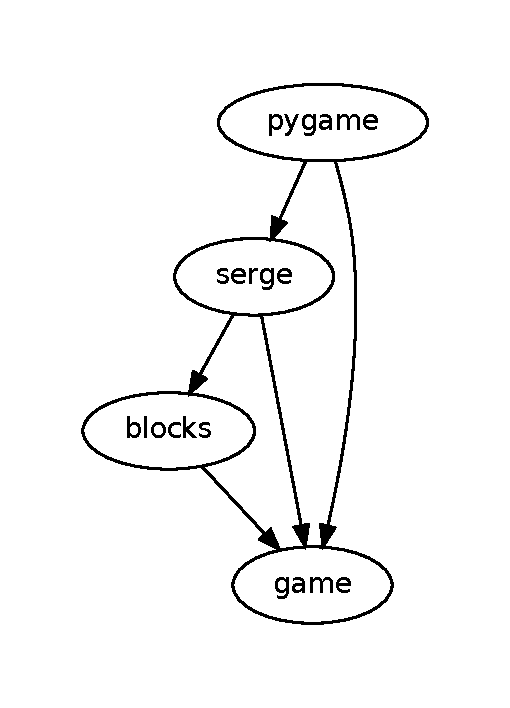
\includegraphics{graphviz-e105d178f146796d84ac12b606890fb9e5d18932.pdf}

Typical game folder structure for a game.

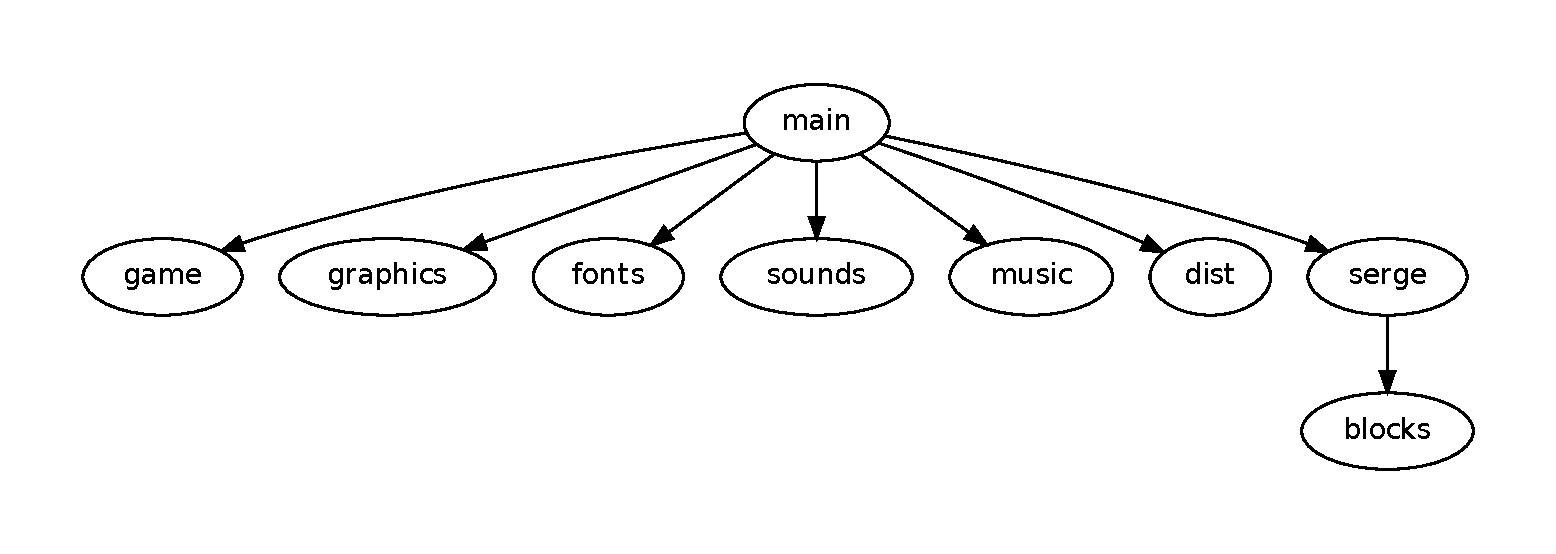
\includegraphics{graphviz-0adf03b837469c93904cfb93fe55dd097116c3d6.pdf}

Engine Structure.

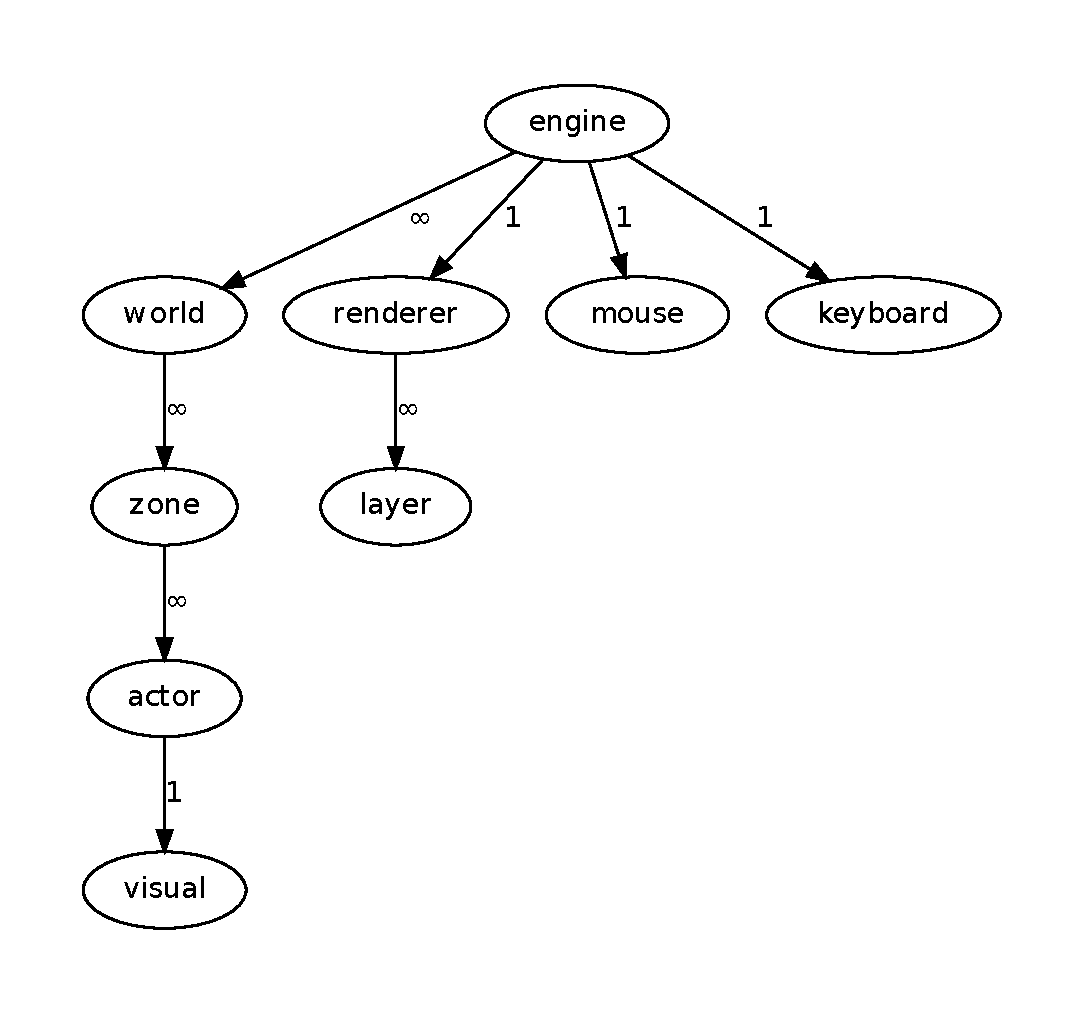
\includegraphics{graphviz-e2e822b8a37c9284baaff76adbf1821ec6eb1438.pdf}

Typical game flow.
\par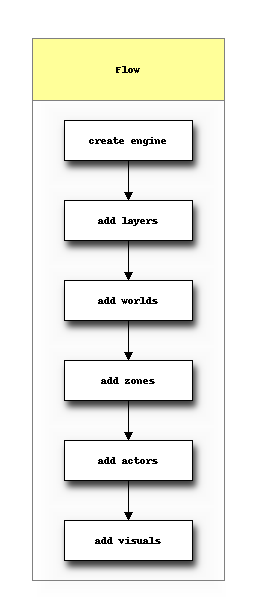
\includegraphics{actdiag-fc87f097c5ab00ddb68ee1091b95b8b7d891992a.png}\par
Class Structures:


\chapter{Engine}
\label{engine:engine}\label{engine::doc}\setbox0\vbox{
\begin{minipage}{0.95\linewidth}
\textbf{Contents}

\medskip

\begin{itemize}
\item {} 
{\hyperref[engine:engine]{Engine}}
\begin{itemize}
\item {} 
{\hyperref[engine:id1]{Engine}}

\item {} 
{\hyperref[engine:enginestats]{EngineStats}}

\end{itemize}

\end{itemize}
\end{minipage}}
\begin{center}\setlength{\fboxsep}{5pt}\shadowbox{\box0}\end{center}
\phantomsection\label{engine:module-engine}\index{engine (module)}

\section{Engine}
\label{engine:id1}\index{Engine (class in serge.engine)}

\begin{fulllineitems}
\phantomsection\label{engine:serge.engine.Engine}\pysiglinewithargsret{\strong{class }\code{serge.engine.}\bfcode{Engine}}{\emph{width=640}, \emph{height=480}, \emph{title='Serge'}, \emph{backcolour=(0}, \emph{0}, \emph{0)}, \emph{icon=None}, \emph{fullscreen=False}}{}
Bases: {\hyperref[common:serge.common.Loggable]{\code{serge.common.Loggable}}}, {\hyperref[common:serge.serialize.Serializable]{\code{serge.serialize.Serializable}}}, {\hyperref[common:serge.common.EventAware]{\code{serge.common.EventAware}}}

The main Serge engine

The engine manages a set of worlds and allows
a single {\hyperref[world::doc]{\emph{Worlds}}}, the current world, to be automatically
updated on a certain time frequency.
\index{addWorld() (serge.engine.Engine method)}

\begin{fulllineitems}
\phantomsection\label{engine:serge.engine.Engine.addWorld}\pysiglinewithargsret{\bfcode{addWorld}}{\emph{world}}{}
Add a world to the engine
\begin{quote}\begin{description}
\item[{Parameters}] \leavevmode
\textbf{world} -- the world instance to add

\end{description}\end{quote}

\end{fulllineitems}

\index{attachBuilder() (serge.engine.Engine method)}

\begin{fulllineitems}
\phantomsection\label{engine:serge.engine.Engine.attachBuilder}\pysiglinewithargsret{\bfcode{attachBuilder}}{\emph{builder}}{}
Attach a builder

\end{fulllineitems}

\index{clearWorlds() (serge.engine.Engine method)}

\begin{fulllineitems}
\phantomsection\label{engine:serge.engine.Engine.clearWorlds}\pysiglinewithargsret{\bfcode{clearWorlds}}{}{}
Clear all the worlds

\end{fulllineitems}

\index{detachBuilder() (serge.engine.Engine method)}

\begin{fulllineitems}
\phantomsection\label{engine:serge.engine.Engine.detachBuilder}\pysiglinewithargsret{\bfcode{detachBuilder}}{}{}
Detach the builder

\end{fulllineitems}

\index{getCurrentWorld() (serge.engine.Engine method)}

\begin{fulllineitems}
\phantomsection\label{engine:serge.engine.Engine.getCurrentWorld}\pysiglinewithargsret{\bfcode{getCurrentWorld}}{}{}
Return the currently selected world

\end{fulllineitems}

\index{getKeyboard() (serge.engine.Engine method)}

\begin{fulllineitems}
\phantomsection\label{engine:serge.engine.Engine.getKeyboard}\pysiglinewithargsret{\bfcode{getKeyboard}}{}{}
Return the keyboard

\end{fulllineitems}

\index{getMouse() (serge.engine.Engine method)}

\begin{fulllineitems}
\phantomsection\label{engine:serge.engine.Engine.getMouse}\pysiglinewithargsret{\bfcode{getMouse}}{}{}
Return the mouse

\end{fulllineitems}

\index{getRenderer() (serge.engine.Engine method)}

\begin{fulllineitems}
\phantomsection\label{engine:serge.engine.Engine.getRenderer}\pysiglinewithargsret{\bfcode{getRenderer}}{}{}
Return the renderer

\end{fulllineitems}

\index{getSprites() (serge.engine.Engine method)}

\begin{fulllineitems}
\phantomsection\label{engine:serge.engine.Engine.getSprites}\pysiglinewithargsret{\bfcode{getSprites}}{}{}
Return the sprite registry

\end{fulllineitems}

\index{getStats() (serge.engine.Engine method)}

\begin{fulllineitems}
\phantomsection\label{engine:serge.engine.Engine.getStats}\pysiglinewithargsret{\bfcode{getStats}}{}{}
Return the stats for the engine

\end{fulllineitems}

\index{getWorld() (serge.engine.Engine method)}

\begin{fulllineitems}
\phantomsection\label{engine:serge.engine.Engine.getWorld}\pysiglinewithargsret{\bfcode{getWorld}}{\emph{name}}{}
Return the named world
\begin{quote}\begin{description}
\item[{Parameters}] \leavevmode
\textbf{name} -- the name of the world to return

\end{description}\end{quote}

\end{fulllineitems}

\index{getWorlds() (serge.engine.Engine method)}

\begin{fulllineitems}
\phantomsection\label{engine:serge.engine.Engine.getWorlds}\pysiglinewithargsret{\bfcode{getWorlds}}{}{}
Return all the worlds

\end{fulllineitems}

\index{goBackToPreviousWorld() (serge.engine.Engine method)}

\begin{fulllineitems}
\phantomsection\label{engine:serge.engine.Engine.goBackToPreviousWorld}\pysiglinewithargsret{\bfcode{goBackToPreviousWorld}}{\emph{obj=None}, \emph{arg=None}}{}
Return to the world we were in before this one

The arguments are never used and are just here to allow you to use
this method as an event callback.

\end{fulllineitems}

\index{init() (serge.engine.Engine method)}

\begin{fulllineitems}
\phantomsection\label{engine:serge.engine.Engine.init}\pysiglinewithargsret{\bfcode{init}}{}{}
Initialise ourself

\end{fulllineitems}

\index{processEvents() (serge.engine.Engine method)}

\begin{fulllineitems}
\phantomsection\label{engine:serge.engine.Engine.processEvents}\pysiglinewithargsret{\bfcode{processEvents}}{}{}
Process all the events for the current world

\end{fulllineitems}

\index{removeWorld() (serge.engine.Engine method)}

\begin{fulllineitems}
\phantomsection\label{engine:serge.engine.Engine.removeWorld}\pysiglinewithargsret{\bfcode{removeWorld}}{\emph{world}}{}
Remove a world from the engine
\begin{quote}\begin{description}
\item[{Parameters}] \leavevmode
\textbf{world} -- the world instance to remove

\end{description}\end{quote}

\end{fulllineitems}

\index{removeWorldNamed() (serge.engine.Engine method)}

\begin{fulllineitems}
\phantomsection\label{engine:serge.engine.Engine.removeWorldNamed}\pysiglinewithargsret{\bfcode{removeWorldNamed}}{\emph{name}}{}
Remove a world with a given name
\begin{quote}\begin{description}
\item[{Parameters}] \leavevmode
\textbf{name} -- the name of the world to remove

\end{description}\end{quote}

\end{fulllineitems}

\index{run() (serge.engine.Engine method)}

\begin{fulllineitems}
\phantomsection\label{engine:serge.engine.Engine.run}\pysiglinewithargsret{\bfcode{run}}{\emph{fps}, \emph{endat=None}}{}
Run the updates at the specified frames per second until the optional endtime
\begin{quote}\begin{description}
\item[{Parameters}] \leavevmode\begin{itemize}
\item {} 
\textbf{fps} -- the target frames per second (integer)

\item {} 
\textbf{endat} -- a time to stop the engine at (long), eg time.time()+60 to run for a minute

\end{itemize}

\end{description}\end{quote}

\end{fulllineitems}

\index{runAsync() (serge.engine.Engine method)}

\begin{fulllineitems}
\phantomsection\label{engine:serge.engine.Engine.runAsync}\pysiglinewithargsret{\bfcode{runAsync}}{\emph{fps}, \emph{endat=None}}{}
Run the engine asynchronously
\begin{quote}\begin{description}
\item[{Parameters}] \leavevmode\begin{itemize}
\item {} 
\textbf{fps} -- the target frames per second (integer)

\item {} 
\textbf{endat} -- a time to stop the engine at (long), eg time.time()+60 to run for a minute

\end{itemize}

\end{description}\end{quote}

\end{fulllineitems}

\index{save() (serge.engine.Engine method)}

\begin{fulllineitems}
\phantomsection\label{engine:serge.engine.Engine.save}\pysiglinewithargsret{\bfcode{save}}{\emph{filename}}{}
Store the engine state in a file suitable for loading again in the furture
\begin{quote}\begin{description}
\item[{Parameters}] \leavevmode
\textbf{filename} -- the name of the file to save into

\end{description}\end{quote}

\end{fulllineitems}

\index{setCurrentWorld() (serge.engine.Engine method)}

\begin{fulllineitems}
\phantomsection\label{engine:serge.engine.Engine.setCurrentWorld}\pysiglinewithargsret{\bfcode{setCurrentWorld}}{\emph{world}}{}
Set the current world
\begin{quote}\begin{description}
\item[{Parameters}] \leavevmode
\textbf{world} -- the world to set as the current world

\end{description}\end{quote}

\end{fulllineitems}

\index{setCurrentWorldByName() (serge.engine.Engine method)}

\begin{fulllineitems}
\phantomsection\label{engine:serge.engine.Engine.setCurrentWorldByName}\pysiglinewithargsret{\bfcode{setCurrentWorldByName}}{\emph{name}}{}
Set the current world to the one with the given name
\begin{quote}\begin{description}
\item[{Parameters}] \leavevmode
\textbf{name} -- the name of the world to set as the current world

\end{description}\end{quote}

\end{fulllineitems}

\index{stop() (serge.engine.Engine method)}

\begin{fulllineitems}
\phantomsection\label{engine:serge.engine.Engine.stop}\pysiglinewithargsret{\bfcode{stop}}{}{}
Stop the engine running

\end{fulllineitems}

\index{updateWorld() (serge.engine.Engine method)}

\begin{fulllineitems}
\phantomsection\label{engine:serge.engine.Engine.updateWorld}\pysiglinewithargsret{\bfcode{updateWorld}}{\emph{interval}}{}
Update the current world

\end{fulllineitems}


\end{fulllineitems}



\section{EngineStats}
\label{engine:enginestats}\index{EngineStats (class in serge.engine)}

\begin{fulllineitems}
\phantomsection\label{engine:serge.engine.EngineStats}\pysigline{\strong{class }\code{serge.engine.}\bfcode{EngineStats}}
Statistic for the engine
\index{afterRender() (serge.engine.EngineStats method)}

\begin{fulllineitems}
\phantomsection\label{engine:serge.engine.EngineStats.afterRender}\pysiglinewithargsret{\bfcode{afterRender}}{}{}
Record that we are after a rendering cycle

\end{fulllineitems}

\index{beforeRender() (serge.engine.EngineStats method)}

\begin{fulllineitems}
\phantomsection\label{engine:serge.engine.EngineStats.beforeRender}\pysiglinewithargsret{\bfcode{beforeRender}}{}{}
Record we are before a rendering cycle

\end{fulllineitems}

\index{recordFrame() (serge.engine.EngineStats method)}

\begin{fulllineitems}
\phantomsection\label{engine:serge.engine.EngineStats.recordFrame}\pysiglinewithargsret{\bfcode{recordFrame}}{}{}
Record a frame

\end{fulllineitems}


\end{fulllineitems}



\chapter{Worlds}
\label{world:worlds}\label{world::doc}

\section{Zones}
\label{zone:zones}\label{zone:module-zone}\label{zone::doc}\index{zone (module)}\index{Zone (class in serge.zone)}

\begin{fulllineitems}
\phantomsection\label{zone:serge.zone.Zone}\pysigline{\strong{class }\code{serge.zone.}\bfcode{Zone}}
Bases: {\hyperref[geometry:serge.geometry.Rectangle]{\code{serge.geometry.Rectangle}}}, {\hyperref[common:serge.common.Loggable]{\code{serge.common.Loggable}}}

A zone

A zone is part of a world. It is a container for objects
and it controls whether objects will take part in world 
updates.
\index{addActor() (serge.zone.Zone method)}

\begin{fulllineitems}
\phantomsection\label{zone:serge.zone.Zone.addActor}\pysiglinewithargsret{\bfcode{addActor}}{\emph{actor}}{}
Add an actor to the zone

\end{fulllineitems}

\index{clearActors() (serge.zone.Zone method)}

\begin{fulllineitems}
\phantomsection\label{zone:serge.zone.Zone.clearActors}\pysiglinewithargsret{\bfcode{clearActors}}{}{}
Remove all actors

\end{fulllineitems}

\index{findActorByName() (serge.zone.Zone method)}

\begin{fulllineitems}
\phantomsection\label{zone:serge.zone.Zone.findActorByName}\pysiglinewithargsret{\bfcode{findActorByName}}{\emph{name}}{}
Return the actor with the given name

\end{fulllineitems}

\index{findActorsByTag() (serge.zone.Zone method)}

\begin{fulllineitems}
\phantomsection\label{zone:serge.zone.Zone.findActorsByTag}\pysiglinewithargsret{\bfcode{findActorsByTag}}{\emph{tag}}{}
Return all the actors with a certain tag

\end{fulllineitems}

\index{findFirstActorByTag() (serge.zone.Zone method)}

\begin{fulllineitems}
\phantomsection\label{zone:serge.zone.Zone.findFirstActorByTag}\pysiglinewithargsret{\bfcode{findFirstActorByTag}}{\emph{tag}}{}
Return the first actor found with the given tag or raise an error

\end{fulllineitems}

\index{getActors() (serge.zone.Zone method)}

\begin{fulllineitems}
\phantomsection\label{zone:serge.zone.Zone.getActors}\pysiglinewithargsret{\bfcode{getActors}}{}{}
Return all the actors

\end{fulllineitems}

\index{hasActor() (serge.zone.Zone method)}

\begin{fulllineitems}
\phantomsection\label{zone:serge.zone.Zone.hasActor}\pysiglinewithargsret{\bfcode{hasActor}}{\emph{actor}}{}
Return True if the actor is in this zone

\end{fulllineitems}

\index{init() (serge.zone.Zone method)}

\begin{fulllineitems}
\phantomsection\label{zone:serge.zone.Zone.init}\pysiglinewithargsret{\bfcode{init}}{}{}
Initialise from serialized state

\end{fulllineitems}

\index{removeActor() (serge.zone.Zone method)}

\begin{fulllineitems}
\phantomsection\label{zone:serge.zone.Zone.removeActor}\pysiglinewithargsret{\bfcode{removeActor}}{\emph{actor}}{}
Remove an actor from the zone

\end{fulllineitems}

\index{setGlobalForce() (serge.zone.Zone method)}

\begin{fulllineitems}
\phantomsection\label{zone:serge.zone.Zone.setGlobalForce}\pysiglinewithargsret{\bfcode{setGlobalForce}}{\emph{force}}{}
Set the global force for physics

\end{fulllineitems}

\index{setPhysicsStepsize() (serge.zone.Zone method)}

\begin{fulllineitems}
\phantomsection\label{zone:serge.zone.Zone.setPhysicsStepsize}\pysiglinewithargsret{\bfcode{setPhysicsStepsize}}{\emph{interval}}{}
Set the maximum step size for physics calculations

\end{fulllineitems}

\index{sleepActor() (serge.zone.Zone method)}

\begin{fulllineitems}
\phantomsection\label{zone:serge.zone.Zone.sleepActor}\pysiglinewithargsret{\bfcode{sleepActor}}{\emph{actor}}{}
Tell the actor to go to sleep from a physics perspective

The actor will still be visible and will still be updated but it
will not update its physics. Useful for optimising when an actor
does not need to interact with the physics simulation for a while.

\end{fulllineitems}

\index{updatePhysics() (serge.zone.Zone method)}

\begin{fulllineitems}
\phantomsection\label{zone:serge.zone.Zone.updatePhysics}\pysiglinewithargsret{\bfcode{updatePhysics}}{\emph{interval}}{}
Perform a step of the physics engine

You do not normally need to call this method as it is called by the
updateZone method. You may call this to advance the physics simulation
along without affecting other game elements.

\end{fulllineitems}

\index{updateZone() (serge.zone.Zone method)}

\begin{fulllineitems}
\phantomsection\label{zone:serge.zone.Zone.updateZone}\pysiglinewithargsret{\bfcode{updateZone}}{\emph{interval}, \emph{world}}{}
Update the objects in the zone

\end{fulllineitems}

\index{wakeActor() (serge.zone.Zone method)}

\begin{fulllineitems}
\phantomsection\label{zone:serge.zone.Zone.wakeActor}\pysiglinewithargsret{\bfcode{wakeActor}}{\emph{actor}}{}
Tell the actor to go to wake up from a physics perspective

An actor that was put to sleep (via sleepActor) will be woken
up and take part in the physics simulation again.

\end{fulllineitems}

\index{wouldContain() (serge.zone.Zone method)}

\begin{fulllineitems}
\phantomsection\label{zone:serge.zone.Zone.wouldContain}\pysiglinewithargsret{\bfcode{wouldContain}}{\emph{actor}}{}
Return True if this zone would contain the actor as it is right now

The base Zone implementation uses spatial overlapping as the criteria but you
can create custom zones that use other criteria to decide which actors should
be in the zone.

\end{fulllineitems}


\end{fulllineitems}



\section{Actors}
\label{actor:actors}\label{actor::doc}\setbox0\vbox{
\begin{minipage}{0.95\linewidth}
\textbf{Contents}

\medskip

\begin{itemize}
\item {} 
{\hyperref[actor:actors]{Actors}}
\begin{itemize}
\item {} 
{\hyperref[actor:actor]{Actor}}

\item {} 
{\hyperref[actor:compositeactor]{CompositeActor}}

\item {} 
{\hyperref[actor:mountableactor]{MountableActor}}

\item {} 
{\hyperref[actor:physicallymountableactor]{PhysicallyMountableActor}}

\item {} 
{\hyperref[actor:actorcollection]{ActorCollection}}

\end{itemize}

\end{itemize}
\end{minipage}}
\begin{center}\setlength{\fboxsep}{5pt}\shadowbox{\box0}\end{center}
\phantomsection\label{actor:module-actor}\index{actor (module)}

\subsection{Actor}
\label{actor:actor}
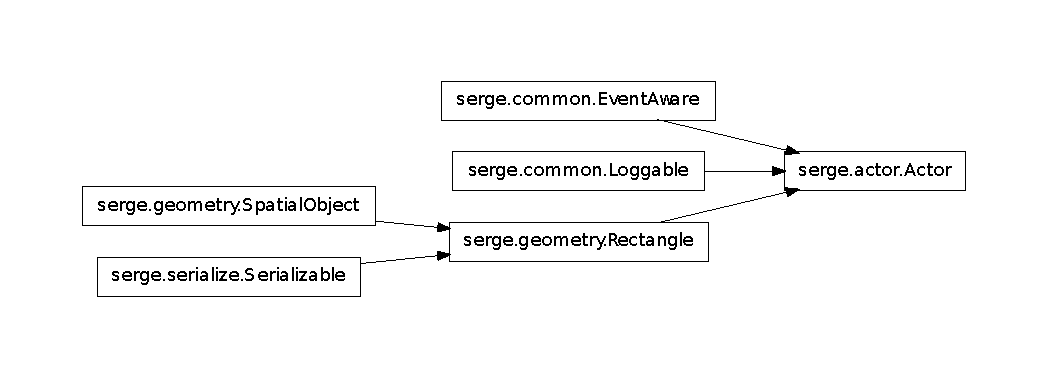
\includegraphics{inheritance-746dcf96db11da32828c60c2bdb88bb47e0a7e89.pdf}
\index{Actor (class in serge.actor)}

\begin{fulllineitems}
\phantomsection\label{actor:serge.actor.Actor}\pysiglinewithargsret{\strong{class }\code{serge.actor.}\bfcode{Actor}}{\emph{tag}, \emph{name='`}}{}
Bases: {\hyperref[common:serge.common.Loggable]{\code{serge.common.Loggable}}}, {\hyperref[geometry:serge.geometry.Rectangle]{\code{serge.geometry.Rectangle}}}, {\hyperref[common:serge.common.EventAware]{\code{serge.common.EventAware}}}

Represents an actor
\index{addedToWorld() (serge.actor.Actor method)}

\begin{fulllineitems}
\phantomsection\label{actor:serge.actor.Actor.addedToWorld}\pysiglinewithargsret{\bfcode{addedToWorld}}{\emph{world}}{}
Called when we are being added to the world

\end{fulllineitems}

\index{getAngle() (serge.actor.Actor method)}

\begin{fulllineitems}
\phantomsection\label{actor:serge.actor.Actor.getAngle}\pysiglinewithargsret{\bfcode{getAngle}}{}{}
Return the angle for the actor

\end{fulllineitems}

\index{getLayerName() (serge.actor.Actor method)}

\begin{fulllineitems}
\phantomsection\label{actor:serge.actor.Actor.getLayerName}\pysiglinewithargsret{\bfcode{getLayerName}}{}{}
Return our layer name

\end{fulllineitems}

\index{getNiceName() (serge.actor.Actor method)}

\begin{fulllineitems}
\phantomsection\label{actor:serge.actor.Actor.getNiceName}\pysiglinewithargsret{\bfcode{getNiceName}}{}{}
Return a nice name for this actor

\end{fulllineitems}

\index{getPhysical() (serge.actor.Actor method)}

\begin{fulllineitems}
\phantomsection\label{actor:serge.actor.Actor.getPhysical}\pysiglinewithargsret{\bfcode{getPhysical}}{}{}
Return the physical conditions

\end{fulllineitems}

\index{getSpriteName() (serge.actor.Actor method)}

\begin{fulllineitems}
\phantomsection\label{actor:serge.actor.Actor.getSpriteName}\pysiglinewithargsret{\bfcode{getSpriteName}}{}{}
Return our sprite

\end{fulllineitems}

\index{init() (serge.actor.Actor method)}

\begin{fulllineitems}
\phantomsection\label{actor:serge.actor.Actor.init}\pysiglinewithargsret{\bfcode{init}}{}{}
Initialize from serialized form

\end{fulllineitems}

\index{move() (serge.actor.Actor method)}

\begin{fulllineitems}
\phantomsection\label{actor:serge.actor.Actor.move}\pysiglinewithargsret{\bfcode{move}}{\emph{x}, \emph{y}}{}
Move by a certain amount

\end{fulllineitems}

\index{moveTo() (serge.actor.Actor method)}

\begin{fulllineitems}
\phantomsection\label{actor:serge.actor.Actor.moveTo}\pysiglinewithargsret{\bfcode{moveTo}}{\emph{x}, \emph{y}, \emph{no\_sync=False}, \emph{override\_lock=False}}{}
Move the center of this actor to the given location, unless it is locked

You can override the lock by passing True to override lock.

\end{fulllineitems}

\index{removedFromWorld() (serge.actor.Actor method)}

\begin{fulllineitems}
\phantomsection\label{actor:serge.actor.Actor.removedFromWorld}\pysiglinewithargsret{\bfcode{removedFromWorld}}{\emph{world}}{}
Called when we are being removed from the world

\end{fulllineitems}

\index{renderTo() (serge.actor.Actor method)}

\begin{fulllineitems}
\phantomsection\label{actor:serge.actor.Actor.renderTo}\pysiglinewithargsret{\bfcode{renderTo}}{\emph{renderer}, \emph{interval}}{}
Render ourself to the given renderer

\end{fulllineitems}

\index{setAngle() (serge.actor.Actor method)}

\begin{fulllineitems}
\phantomsection\label{actor:serge.actor.Actor.setAngle}\pysiglinewithargsret{\bfcode{setAngle}}{\emph{angle}, \emph{sync\_physical=False}, \emph{override\_lock=False}}{}
Set the angle for the visual

\end{fulllineitems}

\index{setLayerName() (serge.actor.Actor method)}

\begin{fulllineitems}
\phantomsection\label{actor:serge.actor.Actor.setLayerName}\pysiglinewithargsret{\bfcode{setLayerName}}{\emph{name}}{}
Set the layer that we render to

\end{fulllineitems}

\index{setPhysical() (serge.actor.Actor method)}

\begin{fulllineitems}
\phantomsection\label{actor:serge.actor.Actor.setPhysical}\pysiglinewithargsret{\bfcode{setPhysical}}{\emph{physical\_conditions}}{}
Set the physical conditions

\end{fulllineitems}

\index{setSpriteName() (serge.actor.Actor method)}

\begin{fulllineitems}
\phantomsection\label{actor:serge.actor.Actor.setSpriteName}\pysiglinewithargsret{\bfcode{setSpriteName}}{\emph{name}}{}
Set the sprite for this actor

\end{fulllineitems}

\index{setZoom() (serge.actor.Actor method)}

\begin{fulllineitems}
\phantomsection\label{actor:serge.actor.Actor.setZoom}\pysiglinewithargsret{\bfcode{setZoom}}{\emph{zoom}}{}
Zoom in on this actor

\end{fulllineitems}

\index{syncPhysics() (serge.actor.Actor method)}

\begin{fulllineitems}
\phantomsection\label{actor:serge.actor.Actor.syncPhysics}\pysiglinewithargsret{\bfcode{syncPhysics}}{\emph{spatial\_only=False}}{}
Sync physics when the actors physical properties have been changed

\end{fulllineitems}

\index{updateActor() (serge.actor.Actor method)}

\begin{fulllineitems}
\phantomsection\label{actor:serge.actor.Actor.updateActor}\pysiglinewithargsret{\bfcode{updateActor}}{\emph{interval}, \emph{world}}{}
Update the actor status

\end{fulllineitems}


\end{fulllineitems}



\subsection{CompositeActor}
\label{actor:compositeactor}
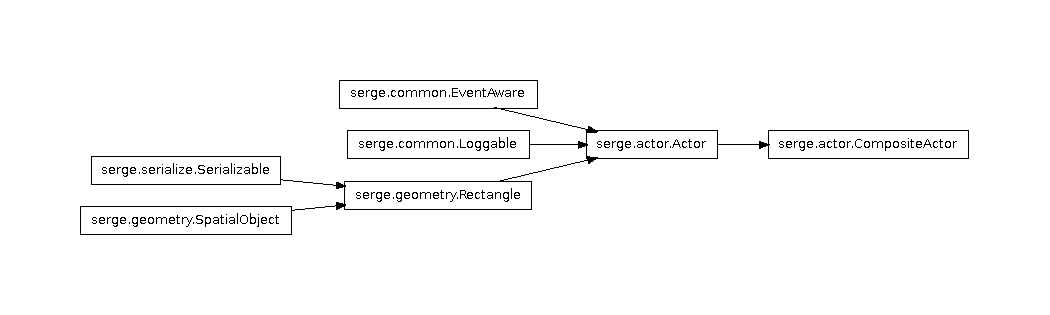
\includegraphics{inheritance-0bf734292bf093de72af693e165c5794f5cd99bc.pdf}
\index{CompositeActor (class in serge.actor)}

\begin{fulllineitems}
\phantomsection\label{actor:serge.actor.CompositeActor}\pysiglinewithargsret{\strong{class }\code{serge.actor.}\bfcode{CompositeActor}}{\emph{*args}, \emph{**kw}}{}
Bases: {\hyperref[actor:serge.actor.Actor]{\code{serge.actor.Actor}}}

An actor that can have children, which are also actors

World operations on the parent, like adding and removing,
will also apply to the children.

If the children are removed from the parent then they are
also removed from the world.
\index{addChild() (serge.actor.CompositeActor method)}

\begin{fulllineitems}
\phantomsection\label{actor:serge.actor.CompositeActor.addChild}\pysiglinewithargsret{\bfcode{addChild}}{\emph{actor}}{}
Add a child actor

\end{fulllineitems}

\index{addedToWorld() (serge.actor.CompositeActor method)}

\begin{fulllineitems}
\phantomsection\label{actor:serge.actor.CompositeActor.addedToWorld}\pysiglinewithargsret{\bfcode{addedToWorld}}{\emph{world}}{}
Called when we are being added to the world

\end{fulllineitems}

\index{getChildren() (serge.actor.CompositeActor method)}

\begin{fulllineitems}
\phantomsection\label{actor:serge.actor.CompositeActor.getChildren}\pysiglinewithargsret{\bfcode{getChildren}}{}{}
Return the list of children

\end{fulllineitems}

\index{getChildrenWithTag() (serge.actor.CompositeActor method)}

\begin{fulllineitems}
\phantomsection\label{actor:serge.actor.CompositeActor.getChildrenWithTag}\pysiglinewithargsret{\bfcode{getChildrenWithTag}}{\emph{tag}}{}
Return all the children with a certain tag

\end{fulllineitems}

\index{hasChild() (serge.actor.CompositeActor method)}

\begin{fulllineitems}
\phantomsection\label{actor:serge.actor.CompositeActor.hasChild}\pysiglinewithargsret{\bfcode{hasChild}}{\emph{actor}}{}
Return True if this actor already has this actor as a child

\end{fulllineitems}

\index{hasChildren() (serge.actor.CompositeActor method)}

\begin{fulllineitems}
\phantomsection\label{actor:serge.actor.CompositeActor.hasChildren}\pysiglinewithargsret{\bfcode{hasChildren}}{}{}
Return True if this actor has children

\end{fulllineitems}

\index{removeChild() (serge.actor.CompositeActor method)}

\begin{fulllineitems}
\phantomsection\label{actor:serge.actor.CompositeActor.removeChild}\pysiglinewithargsret{\bfcode{removeChild}}{\emph{actor}, \emph{leave\_in\_world=False}}{}
Remove a child actor

\end{fulllineitems}

\index{removeChildren() (serge.actor.CompositeActor method)}

\begin{fulllineitems}
\phantomsection\label{actor:serge.actor.CompositeActor.removeChildren}\pysiglinewithargsret{\bfcode{removeChildren}}{}{}
Remove all the children

\end{fulllineitems}

\index{removedFromWorld() (serge.actor.CompositeActor method)}

\begin{fulllineitems}
\phantomsection\label{actor:serge.actor.CompositeActor.removedFromWorld}\pysiglinewithargsret{\bfcode{removedFromWorld}}{\emph{world}}{}
Called when we are being removed from the world

\end{fulllineitems}


\end{fulllineitems}



\subsection{MountableActor}
\label{actor:mountableactor}
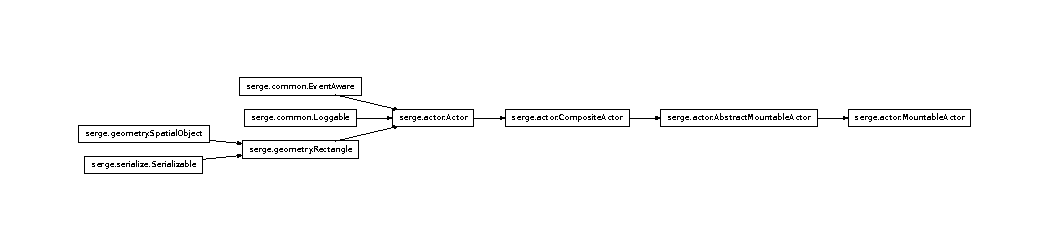
\includegraphics{inheritance-a5b8c8041a7dda9bc1cee193da3149de85ddbd9b.pdf}
\index{MountableActor (class in serge.actor)}

\begin{fulllineitems}
\phantomsection\label{actor:serge.actor.MountableActor}\pysiglinewithargsret{\strong{class }\code{serge.actor.}\bfcode{MountableActor}}{\emph{*args}, \emph{**kw}}{}
Bases: \code{serge.actor.AbstractMountableActor}

An actor that you can mount other actors to

The other actors are located at a certain position
relative to the position of this actor. You can
use this actor to create clusters either visually
or functionally.
\index{moveTo() (serge.actor.MountableActor method)}

\begin{fulllineitems}
\phantomsection\label{actor:serge.actor.MountableActor.moveTo}\pysiglinewithargsret{\bfcode{moveTo}}{\emph{x}, \emph{y}, \emph{no\_sync=False}, \emph{override\_lock=False}}{}
Move this actor

\end{fulllineitems}

\index{setAngle() (serge.actor.MountableActor method)}

\begin{fulllineitems}
\phantomsection\label{actor:serge.actor.MountableActor.setAngle}\pysiglinewithargsret{\bfcode{setAngle}}{\emph{angle}, \emph{sync\_physical=False}, \emph{override\_lock=False}}{}
Set the angle for the visual

\end{fulllineitems}


\end{fulllineitems}



\subsection{PhysicallyMountableActor}
\label{actor:physicallymountableactor}
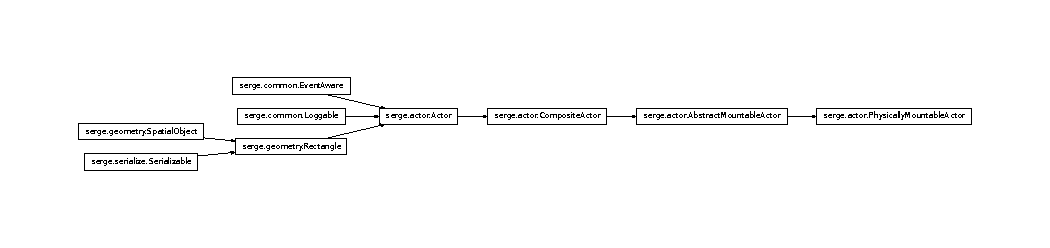
\includegraphics{inheritance-215be21f1f2a46f6eb668bf702c8a1a7040e871b.pdf}
\index{PhysicallyMountableActor (class in serge.actor)}

\begin{fulllineitems}
\phantomsection\label{actor:serge.actor.PhysicallyMountableActor}\pysiglinewithargsret{\strong{class }\code{serge.actor.}\bfcode{PhysicallyMountableActor}}{\emph{tag}, \emph{name='`}, \emph{mass=0.0}, \emph{**kw}}{}
Bases: \code{serge.actor.AbstractMountableActor}

An physical actor that you can mount other physical actors to

The other actors are located at a certain position
relative to the position of this actor. You can
use this actor to create clusters either visually
or functionally.

All actors must be under the control of the physics engine.
\index{addedToWorld() (serge.actor.PhysicallyMountableActor method)}

\begin{fulllineitems}
\phantomsection\label{actor:serge.actor.PhysicallyMountableActor.addedToWorld}\pysiglinewithargsret{\bfcode{addedToWorld}}{\emph{world}}{}
The actor was added to the world

\end{fulllineitems}

\index{init() (serge.actor.PhysicallyMountableActor method)}

\begin{fulllineitems}
\phantomsection\label{actor:serge.actor.PhysicallyMountableActor.init}\pysiglinewithargsret{\bfcode{init}}{}{}
Initialise from serialized form

\end{fulllineitems}

\index{mountActor() (serge.actor.PhysicallyMountableActor method)}

\begin{fulllineitems}
\phantomsection\label{actor:serge.actor.PhysicallyMountableActor.mountActor}\pysiglinewithargsret{\bfcode{mountActor}}{\emph{actor}, \emph{(x}, \emph{y)}, \emph{original\_rotation=False}}{}
Mount the actor with the given offset

\end{fulllineitems}

\index{moveTo() (serge.actor.PhysicallyMountableActor method)}

\begin{fulllineitems}
\phantomsection\label{actor:serge.actor.PhysicallyMountableActor.moveTo}\pysiglinewithargsret{\bfcode{moveTo}}{\emph{x}, \emph{y}, \emph{no\_sync=False}, \emph{override\_lock=False}}{}
Move this actor

\end{fulllineitems}

\index{setAngle() (serge.actor.PhysicallyMountableActor method)}

\begin{fulllineitems}
\phantomsection\label{actor:serge.actor.PhysicallyMountableActor.setAngle}\pysiglinewithargsret{\bfcode{setAngle}}{\emph{angle}, \emph{sync\_physical=False}, \emph{override\_lock=False}}{}
Set the angle for the visual

\end{fulllineitems}

\index{unmountActor() (serge.actor.PhysicallyMountableActor method)}

\begin{fulllineitems}
\phantomsection\label{actor:serge.actor.PhysicallyMountableActor.unmountActor}\pysiglinewithargsret{\bfcode{unmountActor}}{\emph{actor}}{}
Unmount the actor

\end{fulllineitems}


\end{fulllineitems}



\subsection{ActorCollection}
\label{actor:actorcollection}
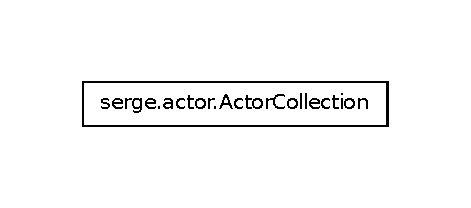
\includegraphics{inheritance-af6282a721309f3c98a915ce735acd55205b815b.pdf}
\index{ActorCollection (class in serge.actor)}

\begin{fulllineitems}
\phantomsection\label{actor:serge.actor.ActorCollection}\pysigline{\strong{class }\code{serge.actor.}\bfcode{ActorCollection}}
Bases: \code{list}

A list of actors

This class implements some useful methods which help to 
handle collections of actors.
\index{findActorByName() (serge.actor.ActorCollection method)}

\begin{fulllineitems}
\phantomsection\label{actor:serge.actor.ActorCollection.findActorByName}\pysiglinewithargsret{\bfcode{findActorByName}}{\emph{name}}{}
Return then actor with the given name

\end{fulllineitems}

\index{findActorsByTag() (serge.actor.ActorCollection method)}

\begin{fulllineitems}
\phantomsection\label{actor:serge.actor.ActorCollection.findActorsByTag}\pysiglinewithargsret{\bfcode{findActorsByTag}}{\emph{tag}}{}
Return a collection of actors with the given tag

\end{fulllineitems}

\index{findActorsByTags() (serge.actor.ActorCollection method)}

\begin{fulllineitems}
\phantomsection\label{actor:serge.actor.ActorCollection.findActorsByTags}\pysiglinewithargsret{\bfcode{findActorsByTags}}{\emph{tags}}{}
Return a collection of actors with at least one of the tags

\end{fulllineitems}

\index{forEach() (serge.actor.ActorCollection method)}

\begin{fulllineitems}
\phantomsection\label{actor:serge.actor.ActorCollection.forEach}\pysiglinewithargsret{\bfcode{forEach}}{}{}
Returns an object suitable for mapping method calls to all the actors in the collection
\begin{description}
\item[{Use this like,}] \leavevmode
collection.forEach().setAngle(12)

\end{description}

\end{fulllineitems}

\index{hasActor() (serge.actor.ActorCollection method)}

\begin{fulllineitems}
\phantomsection\label{actor:serge.actor.ActorCollection.hasActor}\pysiglinewithargsret{\bfcode{hasActor}}{\emph{actor}}{}
Return True if we have that actor

\end{fulllineitems}

\index{hasActorWithName() (serge.actor.ActorCollection method)}

\begin{fulllineitems}
\phantomsection\label{actor:serge.actor.ActorCollection.hasActorWithName}\pysiglinewithargsret{\bfcode{hasActorWithName}}{\emph{name}}{}
Return True if the collection contains an actor with the given name

\end{fulllineitems}

\index{hasActorWithTag() (serge.actor.ActorCollection method)}

\begin{fulllineitems}
\phantomsection\label{actor:serge.actor.ActorCollection.hasActorWithTag}\pysiglinewithargsret{\bfcode{hasActorWithTag}}{\emph{tag}}{}
Return True if the collection contains an actor with the given tag

\end{fulllineitems}

\index{numberOfActorsWithName() (serge.actor.ActorCollection method)}

\begin{fulllineitems}
\phantomsection\label{actor:serge.actor.ActorCollection.numberOfActorsWithName}\pysiglinewithargsret{\bfcode{numberOfActorsWithName}}{\emph{name}}{}
Return the number of actors with the given name

\end{fulllineitems}

\index{numberOfActorsWithTag() (serge.actor.ActorCollection method)}

\begin{fulllineitems}
\phantomsection\label{actor:serge.actor.ActorCollection.numberOfActorsWithTag}\pysiglinewithargsret{\bfcode{numberOfActorsWithTag}}{\emph{tag}}{}
Return the number of actors with the given tag

\end{fulllineitems}


\end{fulllineitems}

\phantomsection\label{world:module-world}\index{world (module)}

\section{World}
\label{world:world}\index{World (class in serge.world)}

\begin{fulllineitems}
\phantomsection\label{world:serge.world.World}\pysiglinewithargsret{\strong{class }\code{serge.world.}\bfcode{World}}{\emph{name}}{}
Bases: {\hyperref[common:serge.common.Loggable]{\code{serge.common.Loggable}}}, {\hyperref[common:serge.serialize.Serializable]{\code{serge.serialize.Serializable}}}, {\hyperref[common:serge.common.EventAware]{\code{serge.common.EventAware}}}

The main world object

The {\hyperref[engine::doc]{\emph{Engine}}} will control main worlds. Each world has a number
of {\hyperref[zone::doc]{\emph{Zones}}} which contain {\hyperref[actor::doc]{\emph{Actors}}}.
\index{activateWorld() (serge.world.World method)}

\begin{fulllineitems}
\phantomsection\label{world:serge.world.World.activateWorld}\pysiglinewithargsret{\bfcode{activateWorld}}{}{}
Called when the world is set as the current world

\end{fulllineitems}

\index{addActor() (serge.world.World method)}

\begin{fulllineitems}
\phantomsection\label{world:serge.world.World.addActor}\pysiglinewithargsret{\bfcode{addActor}}{\emph{actor}}{}
Add an actor to the world

\end{fulllineitems}

\index{addZone() (serge.world.World method)}

\begin{fulllineitems}
\phantomsection\label{world:serge.world.World.addZone}\pysiglinewithargsret{\bfcode{addZone}}{\emph{zone}}{}
Add a zone to the world

\end{fulllineitems}

\index{clearActors() (serge.world.World method)}

\begin{fulllineitems}
\phantomsection\label{world:serge.world.World.clearActors}\pysiglinewithargsret{\bfcode{clearActors}}{}{}
Clear all the actors

\end{fulllineitems}

\index{clearActorsExceptTags() (serge.world.World method)}

\begin{fulllineitems}
\phantomsection\label{world:serge.world.World.clearActorsExceptTags}\pysiglinewithargsret{\bfcode{clearActorsExceptTags}}{\emph{tags}}{}
Clear all actors except the ones with a tag in the list of tags

\end{fulllineitems}

\index{clearActorsWithTags() (serge.world.World method)}

\begin{fulllineitems}
\phantomsection\label{world:serge.world.World.clearActorsWithTags}\pysiglinewithargsret{\bfcode{clearActorsWithTags}}{\emph{tags}}{}
Clear all actors with a tag in the list of tags

\end{fulllineitems}

\index{clearZones() (serge.world.World method)}

\begin{fulllineitems}
\phantomsection\label{world:serge.world.World.clearZones}\pysiglinewithargsret{\bfcode{clearZones}}{}{}
Remove all the zones

\end{fulllineitems}

\index{deactivateWorld() (serge.world.World method)}

\begin{fulllineitems}
\phantomsection\label{world:serge.world.World.deactivateWorld}\pysiglinewithargsret{\bfcode{deactivateWorld}}{}{}
Called when the world is deactivated

\end{fulllineitems}

\index{findActorByName() (serge.world.World method)}

\begin{fulllineitems}
\phantomsection\label{world:serge.world.World.findActorByName}\pysiglinewithargsret{\bfcode{findActorByName}}{\emph{name}}{}
Return the actor with the give name in all zones

\end{fulllineitems}

\index{findActorsAt() (serge.world.World method)}

\begin{fulllineitems}
\phantomsection\label{world:serge.world.World.findActorsAt}\pysiglinewithargsret{\bfcode{findActorsAt}}{\emph{x}, \emph{y}}{}
Return the actors at a certain location

\end{fulllineitems}

\index{findActorsByTag() (serge.world.World method)}

\begin{fulllineitems}
\phantomsection\label{world:serge.world.World.findActorsByTag}\pysiglinewithargsret{\bfcode{findActorsByTag}}{\emph{tag}}{}
Return all the actors in all zones based on the tag

\end{fulllineitems}

\index{getActors() (serge.world.World method)}

\begin{fulllineitems}
\phantomsection\label{world:serge.world.World.getActors}\pysiglinewithargsret{\bfcode{getActors}}{}{}
Return all the actors

\end{fulllineitems}

\index{getEngine() (serge.world.World method)}

\begin{fulllineitems}
\phantomsection\label{world:serge.world.World.getEngine}\pysiglinewithargsret{\bfcode{getEngine}}{}{}
Return the engine that we are owned by

\end{fulllineitems}

\index{hasActor() (serge.world.World method)}

\begin{fulllineitems}
\phantomsection\label{world:serge.world.World.hasActor}\pysiglinewithargsret{\bfcode{hasActor}}{\emph{actor}}{}
Return True if this actor is in the world

\end{fulllineitems}

\index{init() (serge.world.World method)}

\begin{fulllineitems}
\phantomsection\label{world:serge.world.World.init}\pysiglinewithargsret{\bfcode{init}}{}{}
Initialise from serialized state

\end{fulllineitems}

\index{processEvents() (serge.world.World method)}

\begin{fulllineitems}
\phantomsection\label{world:serge.world.World.processEvents}\pysiglinewithargsret{\bfcode{processEvents}}{\emph{events}}{}
Handle the events

\end{fulllineitems}

\index{removeActor() (serge.world.World method)}

\begin{fulllineitems}
\phantomsection\label{world:serge.world.World.removeActor}\pysiglinewithargsret{\bfcode{removeActor}}{\emph{actor}}{}
Remove the actor from the world

\end{fulllineitems}

\index{renderTo() (serge.world.World method)}

\begin{fulllineitems}
\phantomsection\label{world:serge.world.World.renderTo}\pysiglinewithargsret{\bfcode{renderTo}}{\emph{renderer}, \emph{interval}}{}
Render all of our actors in active zones

\end{fulllineitems}

\index{rezoneActors() (serge.world.World method)}

\begin{fulllineitems}
\phantomsection\label{world:serge.world.World.rezoneActors}\pysiglinewithargsret{\bfcode{rezoneActors}}{}{}
Move actors to the right zone based on their spatial location

\end{fulllineitems}

\index{scheduleActorRemoval() (serge.world.World method)}

\begin{fulllineitems}
\phantomsection\label{world:serge.world.World.scheduleActorRemoval}\pysiglinewithargsret{\bfcode{scheduleActorRemoval}}{\emph{actor}}{}
Remove an actor at the end of the next update for the world

This method can be used to safely remove an actor from the world
during the execution of the world update. It can sometimes be
useful to do this when inside logic that is iterating over actors
or inside the updateWorld event loop.

\end{fulllineitems}

\index{setEngine() (serge.world.World method)}

\begin{fulllineitems}
\phantomsection\label{world:serge.world.World.setEngine}\pysiglinewithargsret{\bfcode{setEngine}}{\emph{engine}}{}
Set the engine that we are owned by

\end{fulllineitems}

\index{setGlobalForce() (serge.world.World method)}

\begin{fulllineitems}
\phantomsection\label{world:serge.world.World.setGlobalForce}\pysiglinewithargsret{\bfcode{setGlobalForce}}{\emph{force}}{}
Set the global force for physics

\end{fulllineitems}

\index{setPhysicsStepsize() (serge.world.World method)}

\begin{fulllineitems}
\phantomsection\label{world:serge.world.World.setPhysicsStepsize}\pysiglinewithargsret{\bfcode{setPhysicsStepsize}}{\emph{interval}}{}
Set the maximum step size for physics calculations

\end{fulllineitems}

\index{setZoom() (serge.world.World method)}

\begin{fulllineitems}
\phantomsection\label{world:serge.world.World.setZoom}\pysiglinewithargsret{\bfcode{setZoom}}{\emph{zoom}, \emph{x}, \emph{y}}{}
Set the visual zoom on this world to zoom centered on x, y

\end{fulllineitems}

\index{sleepPhysicsForActors() (serge.world.World method)}

\begin{fulllineitems}
\phantomsection\label{world:serge.world.World.sleepPhysicsForActors}\pysiglinewithargsret{\bfcode{sleepPhysicsForActors}}{\emph{actors}}{}
Tell the actors to go to sleep from a physics perspective

The actors will still be visible and will still be updated but they
will not update their physics. Useful for optimising when an actor
does not need to interact with the physics simulation for a while.

If an actor is unzoned then this will have no impact on them

\end{fulllineitems}

\index{updateWorld() (serge.world.World method)}

\begin{fulllineitems}
\phantomsection\label{world:serge.world.World.updateWorld}\pysiglinewithargsret{\bfcode{updateWorld}}{\emph{interval}}{}
Update the objects in the world

\end{fulllineitems}

\index{wakePhysicsForActors() (serge.world.World method)}

\begin{fulllineitems}
\phantomsection\label{world:serge.world.World.wakePhysicsForActors}\pysiglinewithargsret{\bfcode{wakePhysicsForActors}}{\emph{actors}}{}
Tell the actors to go to wake up from a physics perspective

Actors that were put to sleep (via sleepPhysicsForActors) will be woken
up and take part in the physics simulation again.

\end{fulllineitems}


\end{fulllineitems}



\chapter{Renderering}
\label{renderering:renderering}\label{renderering::doc}\setbox0\vbox{
\begin{minipage}{0.95\linewidth}
\textbf{Contents}

\medskip

\begin{itemize}
\item {} 
{\hyperref[renderering:renderering]{Renderering}}
\begin{itemize}
\item {} 
{\hyperref[renderering:renderer]{Renderer}}

\item {} 
{\hyperref[renderering:layers]{Layers}}
\begin{itemize}
\item {} 
{\hyperref[renderering:renderinglayer]{RenderingLayer}}

\item {} 
{\hyperref[renderering:layer]{Layer}}

\item {} 
{\hyperref[renderering:virtuallayer]{VirtualLayer}}

\end{itemize}

\item {} 
{\hyperref[renderering:cameras]{Cameras}}
\begin{itemize}
\item {} 
{\hyperref[renderering:camera]{Camera}}

\item {} 
{\hyperref[renderering:nullcamera]{NullCamera}}

\end{itemize}

\end{itemize}

\end{itemize}
\end{minipage}}
\begin{center}\setlength{\fboxsep}{5pt}\shadowbox{\box0}\end{center}
\phantomsection\label{renderering:module-camera}\index{camera (module)}\phantomsection\label{renderering:module-render}\index{render (module)}

\section{Renderer}
\label{renderering:renderer}
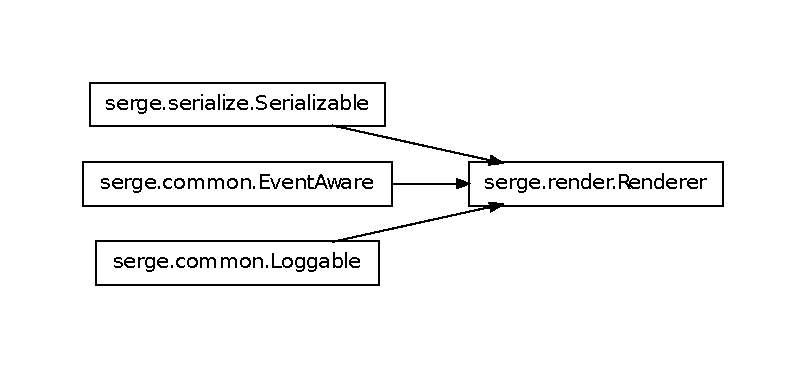
\includegraphics{inheritance-e5a968b60b65c1dac656cd99239cc226c7d7d9f1.pdf}
\index{Renderer (class in serge.render)}

\begin{fulllineitems}
\phantomsection\label{renderering:serge.render.Renderer}\pysiglinewithargsret{\strong{class }\code{serge.render.}\bfcode{Renderer}}{\emph{width=640}, \emph{height=480}, \emph{title='Serge'}, \emph{backcolour=(0}, \emph{0}, \emph{0)}, \emph{icon=None}, \emph{fullscreen=False}}{}
Bases: {\hyperref[common:serge.common.Loggable]{\code{serge.common.Loggable}}}, {\hyperref[common:serge.serialize.Serializable]{\code{serge.serialize.Serializable}}}, {\hyperref[common:serge.common.EventAware]{\code{serge.common.EventAware}}}

The main rendering component
\index{addLayer() (serge.render.Renderer method)}

\begin{fulllineitems}
\phantomsection\label{renderering:serge.render.Renderer.addLayer}\pysiglinewithargsret{\bfcode{addLayer}}{\emph{layer}}{}
Add a layer to the rendering

\end{fulllineitems}

\index{clearLayers() (serge.render.Renderer method)}

\begin{fulllineitems}
\phantomsection\label{renderering:serge.render.Renderer.clearLayers}\pysiglinewithargsret{\bfcode{clearLayers}}{}{}
Clear all the layers

\end{fulllineitems}

\index{clearSurface() (serge.render.Renderer method)}

\begin{fulllineitems}
\phantomsection\label{renderering:serge.render.Renderer.clearSurface}\pysiglinewithargsret{\bfcode{clearSurface}}{}{}
Clear the surface

\end{fulllineitems}

\index{getCamera() (serge.render.Renderer method)}

\begin{fulllineitems}
\phantomsection\label{renderering:serge.render.Renderer.getCamera}\pysiglinewithargsret{\bfcode{getCamera}}{}{}
Return our camera

\end{fulllineitems}

\index{getLayer() (serge.render.Renderer method)}

\begin{fulllineitems}
\phantomsection\label{renderering:serge.render.Renderer.getLayer}\pysiglinewithargsret{\bfcode{getLayer}}{\emph{name}}{}
Return the named layer

\end{fulllineitems}

\index{getLayerBefore() (serge.render.Renderer method)}

\begin{fulllineitems}
\phantomsection\label{renderering:serge.render.Renderer.getLayerBefore}\pysiglinewithargsret{\bfcode{getLayerBefore}}{\emph{layer}}{}
Return the layer before the specified one in terms of rendering order

\end{fulllineitems}

\index{getLayers() (serge.render.Renderer method)}

\begin{fulllineitems}
\phantomsection\label{renderering:serge.render.Renderer.getLayers}\pysiglinewithargsret{\bfcode{getLayers}}{}{}
Return all the layers

\end{fulllineitems}

\index{getScreenSize() (serge.render.Renderer method)}

\begin{fulllineitems}
\phantomsection\label{renderering:serge.render.Renderer.getScreenSize}\pysiglinewithargsret{\bfcode{getScreenSize}}{}{}
Returns the screen size

\end{fulllineitems}

\index{getSurface() (serge.render.Renderer method)}

\begin{fulllineitems}
\phantomsection\label{renderering:serge.render.Renderer.getSurface}\pysiglinewithargsret{\bfcode{getSurface}}{}{}
Return the overall surface

\end{fulllineitems}

\index{init() (serge.render.Renderer method)}

\begin{fulllineitems}
\phantomsection\label{renderering:serge.render.Renderer.init}\pysiglinewithargsret{\bfcode{init}}{}{}
Initialise from serialized state

\end{fulllineitems}

\index{orderActors() (serge.render.Renderer method)}

\begin{fulllineitems}
\phantomsection\label{renderering:serge.render.Renderer.orderActors}\pysiglinewithargsret{\bfcode{orderActors}}{\emph{actors}}{}
Return the list of actors sorted by who should be processed first to correctly render

The actors are checked to see which layer they reside on and then
this is used to order the returned list.

\end{fulllineitems}

\index{preRender() (serge.render.Renderer method)}

\begin{fulllineitems}
\phantomsection\label{renderering:serge.render.Renderer.preRender}\pysiglinewithargsret{\bfcode{preRender}}{}{}
Prepare for new rendering

\end{fulllineitems}

\index{removeLayer() (serge.render.Renderer method)}

\begin{fulllineitems}
\phantomsection\label{renderering:serge.render.Renderer.removeLayer}\pysiglinewithargsret{\bfcode{removeLayer}}{\emph{layer}}{}
Remove the layer from the rendering

\end{fulllineitems}

\index{removeLayerNamed() (serge.render.Renderer method)}

\begin{fulllineitems}
\phantomsection\label{renderering:serge.render.Renderer.removeLayerNamed}\pysiglinewithargsret{\bfcode{removeLayerNamed}}{\emph{name}}{}
Remove the layer with the specific name

\end{fulllineitems}

\index{render() (serge.render.Renderer method)}

\begin{fulllineitems}
\phantomsection\label{renderering:serge.render.Renderer.render}\pysiglinewithargsret{\bfcode{render}}{}{}
Render all the layers

\end{fulllineitems}

\index{resetSurfaces() (serge.render.Renderer method)}

\begin{fulllineitems}
\phantomsection\label{renderering:serge.render.Renderer.resetSurfaces}\pysiglinewithargsret{\bfcode{resetSurfaces}}{}{}
Recreate the surfaces for our layers

When layers are added we sometimes need to reset the layers,
for instance, virtual layers need to be shifted around so
that they have the right order.

\end{fulllineitems}

\index{setCamera() (serge.render.Renderer method)}

\begin{fulllineitems}
\phantomsection\label{renderering:serge.render.Renderer.setCamera}\pysiglinewithargsret{\bfcode{setCamera}}{\emph{camera}}{}
Set our camera

\end{fulllineitems}


\end{fulllineitems}



\section{Layers}
\label{renderering:layers}

\subsection{RenderingLayer}
\label{renderering:renderinglayer}
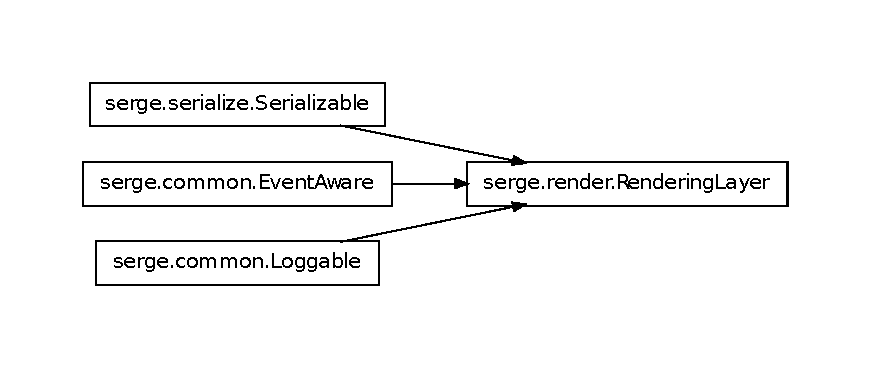
\includegraphics{inheritance-c5d556d35d5d19818ff096f6b93cea35199f7841.pdf}
\index{RenderingLayer (class in serge.render)}

\begin{fulllineitems}
\phantomsection\label{renderering:serge.render.RenderingLayer}\pysiglinewithargsret{\strong{class }\code{serge.render.}\bfcode{RenderingLayer}}{\emph{name}, \emph{order}}{}
Bases: {\hyperref[common:serge.common.Loggable]{\code{serge.common.Loggable}}}, {\hyperref[common:serge.serialize.Serializable]{\code{serge.serialize.Serializable}}}, {\hyperref[common:serge.common.EventAware]{\code{serge.common.EventAware}}}

A layer on which to render things

This is the abstract version of the layer. Create
subclasses of this to do useful things.
\index{clearSurface() (serge.render.RenderingLayer method)}

\begin{fulllineitems}
\phantomsection\label{renderering:serge.render.RenderingLayer.clearSurface}\pysiglinewithargsret{\bfcode{clearSurface}}{}{}
Clear our surface

\end{fulllineitems}

\index{getNiceName() (serge.render.RenderingLayer method)}

\begin{fulllineitems}
\phantomsection\label{renderering:serge.render.RenderingLayer.getNiceName}\pysiglinewithargsret{\bfcode{getNiceName}}{}{}
Return the nice name for this layer

\end{fulllineitems}

\index{getSurface() (serge.render.RenderingLayer method)}

\begin{fulllineitems}
\phantomsection\label{renderering:serge.render.RenderingLayer.getSurface}\pysiglinewithargsret{\bfcode{getSurface}}{}{}
Return the surface

\end{fulllineitems}

\index{init() (serge.render.RenderingLayer method)}

\begin{fulllineitems}
\phantomsection\label{renderering:serge.render.RenderingLayer.init}\pysiglinewithargsret{\bfcode{init}}{}{}
Initialise from serialized state

\end{fulllineitems}

\index{initSurface() (serge.render.RenderingLayer method)}

\begin{fulllineitems}
\phantomsection\label{renderering:serge.render.RenderingLayer.initSurface}\pysiglinewithargsret{\bfcode{initSurface}}{\emph{renderer}}{}
Create the surface that we need to draw on

\end{fulllineitems}

\index{postRender() (serge.render.RenderingLayer method)}

\begin{fulllineitems}
\phantomsection\label{renderering:serge.render.RenderingLayer.postRender}\pysiglinewithargsret{\bfcode{postRender}}{}{}
Called after the layer has has had everything rendered on it

\end{fulllineitems}

\index{preRender() (serge.render.RenderingLayer method)}

\begin{fulllineitems}
\phantomsection\label{renderering:serge.render.RenderingLayer.preRender}\pysiglinewithargsret{\bfcode{preRender}}{}{}
Called before the layer has anything rendered to

\end{fulllineitems}

\index{render() (serge.render.RenderingLayer method)}

\begin{fulllineitems}
\phantomsection\label{renderering:serge.render.RenderingLayer.render}\pysiglinewithargsret{\bfcode{render}}{\emph{surface}}{}
Render to a surface

\end{fulllineitems}

\index{setStatic() (serge.render.RenderingLayer method)}

\begin{fulllineitems}
\phantomsection\label{renderering:serge.render.RenderingLayer.setStatic}\pysiglinewithargsret{\bfcode{setStatic}}{\emph{static}}{}
Determine whether this layer is static with respect to camera movements or not

\end{fulllineitems}

\index{setSurface() (serge.render.RenderingLayer method)}

\begin{fulllineitems}
\phantomsection\label{renderering:serge.render.RenderingLayer.setSurface}\pysiglinewithargsret{\bfcode{setSurface}}{\emph{surface}}{}
Set our surface

\end{fulllineitems}


\end{fulllineitems}



\subsection{Layer}
\label{renderering:layer}
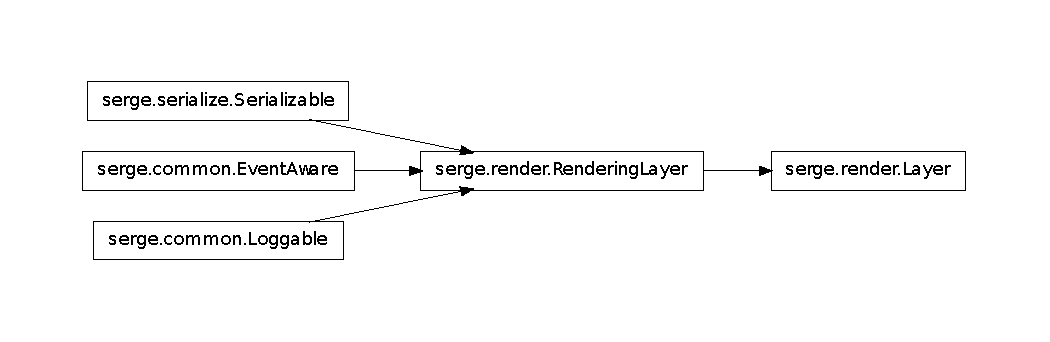
\includegraphics{inheritance-5a62e94f593424d7cc2bac90bb2cd84a200ced64.pdf}
\index{Layer (class in serge.render)}

\begin{fulllineitems}
\phantomsection\label{renderering:serge.render.Layer}\pysiglinewithargsret{\strong{class }\code{serge.render.}\bfcode{Layer}}{\emph{name}, \emph{order}}{}
Bases: {\hyperref[renderering:serge.render.RenderingLayer]{\code{serge.render.RenderingLayer}}}

A rendering layer with its own surface

This type of layer is useful for compositing because
you can do things to this layer once it has been
rendered (eg shadows, glows, blurs etc).
\index{clearSurface() (serge.render.Layer method)}

\begin{fulllineitems}
\phantomsection\label{renderering:serge.render.Layer.clearSurface}\pysiglinewithargsret{\bfcode{clearSurface}}{}{}
Clear our surface

\end{fulllineitems}

\index{initSurface() (serge.render.Layer method)}

\begin{fulllineitems}
\phantomsection\label{renderering:serge.render.Layer.initSurface}\pysiglinewithargsret{\bfcode{initSurface}}{\emph{renderer}}{}
Create the surface that we need to draw on

We create a surface that is identical to the background for the
main renderer.

\end{fulllineitems}

\index{render() (serge.render.Layer method)}

\begin{fulllineitems}
\phantomsection\label{renderering:serge.render.Layer.render}\pysiglinewithargsret{\bfcode{render}}{\emph{surface}}{}
Render to a surface

\end{fulllineitems}


\end{fulllineitems}



\subsection{VirtualLayer}
\label{renderering:virtuallayer}
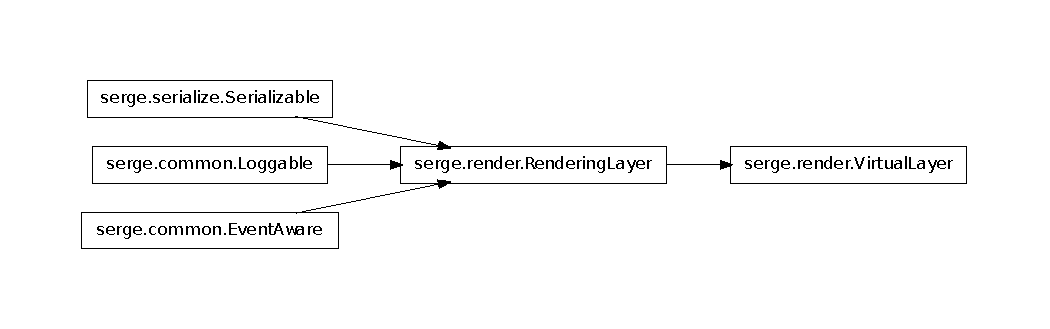
\includegraphics{inheritance-ad19284a075815c08d37d9fbe0742cb1f722b19b.pdf}
\index{VirtualLayer (class in serge.render)}

\begin{fulllineitems}
\phantomsection\label{renderering:serge.render.VirtualLayer}\pysiglinewithargsret{\strong{class }\code{serge.render.}\bfcode{VirtualLayer}}{\emph{name}, \emph{order}}{}
Bases: {\hyperref[renderering:serge.render.RenderingLayer]{\code{serge.render.RenderingLayer}}}

A rendering layer that doesn't have its own surface

This layer will render to the layer immediately
before it in the rendering cycle.
\index{clearSurface() (serge.render.VirtualLayer method)}

\begin{fulllineitems}
\phantomsection\label{renderering:serge.render.VirtualLayer.clearSurface}\pysiglinewithargsret{\bfcode{clearSurface}}{}{}
Clear our surface

Nothing to do here - handled by the real owner of the surface.

\end{fulllineitems}

\index{initSurface() (serge.render.VirtualLayer method)}

\begin{fulllineitems}
\phantomsection\label{renderering:serge.render.VirtualLayer.initSurface}\pysiglinewithargsret{\bfcode{initSurface}}{\emph{renderer}}{}
Create the surface that we need to draw on

We do not want a surface ourself but we need the next surface
in line as far as the renderer is concerned.

\end{fulllineitems}

\index{render() (serge.render.VirtualLayer method)}

\begin{fulllineitems}
\phantomsection\label{renderering:serge.render.VirtualLayer.render}\pysiglinewithargsret{\bfcode{render}}{\emph{surface}}{}
Render to a surface

Nothing to do here - handled by the real owner of the surface.

\end{fulllineitems}


\end{fulllineitems}



\section{Cameras}
\label{renderering:cameras}

\subsection{Camera}
\label{renderering:camera}
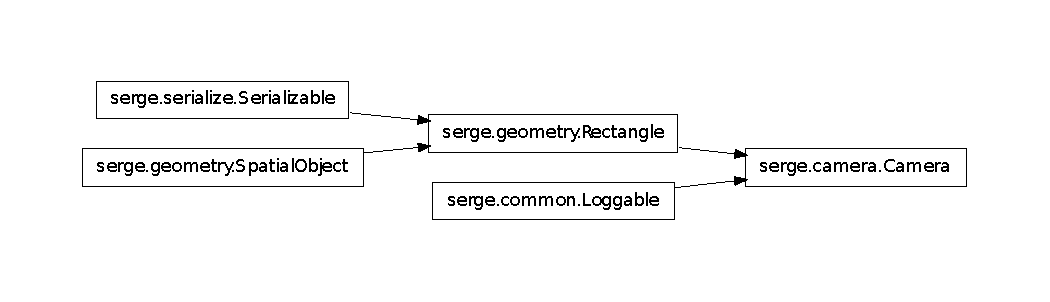
\includegraphics{inheritance-fa5fd197704648001c4011cb69768db04fd90252.pdf}
\index{Camera (class in serge.camera)}

\begin{fulllineitems}
\phantomsection\label{renderering:serge.camera.Camera}\pysigline{\strong{class }\code{serge.camera.}\bfcode{Camera}}
Bases: {\hyperref[common:serge.common.Loggable]{\code{serge.common.Loggable}}}, {\hyperref[geometry:serge.geometry.Rectangle]{\code{serge.geometry.Rectangle}}}

Represents a camera
\index{canSee() (serge.camera.Camera method)}

\begin{fulllineitems}
\phantomsection\label{renderering:serge.camera.Camera.canSee}\pysiglinewithargsret{\bfcode{canSee}}{\emph{actor}}{}
Return True if we can see the actor

\end{fulllineitems}

\index{canSeeActors() (serge.camera.Camera method)}

\begin{fulllineitems}
\phantomsection\label{renderering:serge.camera.Camera.canSeeActors}\pysiglinewithargsret{\bfcode{canSeeActors}}{\emph{actors}}{}
Return the actors that we can see from a list of actors

\end{fulllineitems}

\index{getRelativeLocation() (serge.camera.Camera method)}

\begin{fulllineitems}
\phantomsection\label{renderering:serge.camera.Camera.getRelativeLocation}\pysiglinewithargsret{\bfcode{getRelativeLocation}}{\emph{other}}{}
Return the relative location of one from another

\end{fulllineitems}

\index{getTarget() (serge.camera.Camera method)}

\begin{fulllineitems}
\phantomsection\label{renderering:serge.camera.Camera.getTarget}\pysiglinewithargsret{\bfcode{getTarget}}{}{}
Return the camera's target location

\end{fulllineitems}

\index{init() (serge.camera.Camera method)}

\begin{fulllineitems}
\phantomsection\label{renderering:serge.camera.Camera.init}\pysiglinewithargsret{\bfcode{init}}{}{}
Initialise from serialized

\end{fulllineitems}

\index{setTarget() (serge.camera.Camera method)}

\begin{fulllineitems}
\phantomsection\label{renderering:serge.camera.Camera.setTarget}\pysiglinewithargsret{\bfcode{setTarget}}{\emph{target}}{}
Set the target for the camera to head towards

\end{fulllineitems}

\index{setZoom() (serge.camera.Camera method)}

\begin{fulllineitems}
\phantomsection\label{renderering:serge.camera.Camera.setZoom}\pysiglinewithargsret{\bfcode{setZoom}}{\emph{zoom}, \emph{x}, \emph{y}}{}
Set the new zoom centered on the given x and y

\end{fulllineitems}

\index{update() (serge.camera.Camera method)}

\begin{fulllineitems}
\phantomsection\label{renderering:serge.camera.Camera.update}\pysiglinewithargsret{\bfcode{update}}{\emph{interval}}{}
Update the location of the camera

\end{fulllineitems}


\end{fulllineitems}



\subsection{NullCamera}
\label{renderering:nullcamera}
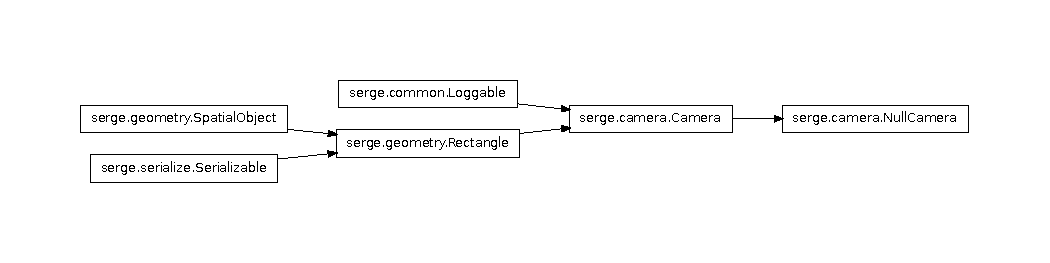
\includegraphics{inheritance-fd4136fac104860ff8c6f5c7355c3df1b33cd442.pdf}
\index{NullCamera (class in serge.camera)}

\begin{fulllineitems}
\phantomsection\label{renderering:serge.camera.NullCamera}\pysigline{\strong{class }\code{serge.camera.}\bfcode{NullCamera}}
Bases: {\hyperref[renderering:serge.camera.Camera]{\code{serge.camera.Camera}}}

A camera that can see everything
\index{canSee() (serge.camera.NullCamera method)}

\begin{fulllineitems}
\phantomsection\label{renderering:serge.camera.NullCamera.canSee}\pysiglinewithargsret{\bfcode{canSee}}{\emph{actor}}{}
Can we see it? Yes we can

\end{fulllineitems}

\index{init() (serge.camera.NullCamera method)}

\begin{fulllineitems}
\phantomsection\label{renderering:serge.camera.NullCamera.init}\pysiglinewithargsret{\bfcode{init}}{}{}
Initialise

\end{fulllineitems}


\end{fulllineitems}



\chapter{Visual}
\label{visual:visual}\label{visual::doc}\setbox0\vbox{
\begin{minipage}{0.95\linewidth}
\textbf{Contents}

\medskip

\begin{itemize}
\item {} 
{\hyperref[visual:visual]{Visual}}
\begin{itemize}
\item {} 
{\hyperref[visual:sprites]{Sprites}}

\item {} 
{\hyperref[visual:fonts]{Fonts}}

\item {} 
{\hyperref[visual:drawing]{Drawing}}

\item {} 
{\hyperref[visual:surfacedrawing]{SurfaceDrawing}}

\item {} 
{\hyperref[visual:sprite]{Sprite}}

\item {} 
{\hyperref[visual:fontstore]{FontStore}}

\item {} 
{\hyperref[visual:store]{Store}}

\item {} 
{\hyperref[visual:text]{Text}}

\end{itemize}

\end{itemize}
\end{minipage}}
\begin{center}\setlength{\fboxsep}{5pt}\shadowbox{\box0}\end{center}
\phantomsection\label{visual:module-visual}\index{visual (module)}

\section{Sprites}
\label{visual:sprites}\index{serge.visual.Sprites (in module visual)}

\begin{fulllineitems}
\phantomsection\label{visual:visual.serge.visual.Sprites}\pysigline{\code{serge.visual.}\bfcode{Sprites}}
Registry of all sprites (is a {\hyperref[visual:store]{Store}})

\end{fulllineitems}



\section{Fonts}
\label{visual:fonts}\index{serge.visual.Fonts (in module visual)}

\begin{fulllineitems}
\phantomsection\label{visual:visual.serge.visual.Fonts}\pysigline{\code{serge.visual.}\bfcode{Fonts}}
Registry of all fonts (is a {\hyperref[visual:fontstore]{FontStore}})

\end{fulllineitems}



\section{Drawing}
\label{visual:drawing}\index{Drawing (class in serge.visual)}

\begin{fulllineitems}
\phantomsection\label{visual:serge.visual.Drawing}\pysigline{\strong{class }\code{serge.visual.}\bfcode{Drawing}}
Bases: \code{object}

Represents something to draw on the screen
\index{flipHorizontal() (serge.visual.Drawing method)}

\begin{fulllineitems}
\phantomsection\label{visual:serge.visual.Drawing.flipHorizontal}\pysiglinewithargsret{\bfcode{flipHorizontal}}{}{}
Flip the drawing horizontally

\end{fulllineitems}

\index{flipVertical() (serge.visual.Drawing method)}

\begin{fulllineitems}
\phantomsection\label{visual:serge.visual.Drawing.flipVertical}\pysiglinewithargsret{\bfcode{flipVertical}}{}{}
Flip the drawing vertically

\end{fulllineitems}

\index{getAngle() (serge.visual.Drawing method)}

\begin{fulllineitems}
\phantomsection\label{visual:serge.visual.Drawing.getAngle}\pysiglinewithargsret{\bfcode{getAngle}}{}{}
Return the current angle

\end{fulllineitems}

\index{getCopy() (serge.visual.Drawing method)}

\begin{fulllineitems}
\phantomsection\label{visual:serge.visual.Drawing.getCopy}\pysiglinewithargsret{\bfcode{getCopy}}{}{}
Return a copy

\end{fulllineitems}

\index{renderTo() (serge.visual.Drawing method)}

\begin{fulllineitems}
\phantomsection\label{visual:serge.visual.Drawing.renderTo}\pysiglinewithargsret{\bfcode{renderTo}}{\emph{milliseconds}, \emph{surface}, \emph{(x}, \emph{y)}}{}
Render to a surface

\end{fulllineitems}

\index{rotateBy() (serge.visual.Drawing method)}

\begin{fulllineitems}
\phantomsection\label{visual:serge.visual.Drawing.rotateBy}\pysiglinewithargsret{\bfcode{rotateBy}}{\emph{angle}}{}
Rotate by a certain amount

\end{fulllineitems}

\index{scaleBy() (serge.visual.Drawing method)}

\begin{fulllineitems}
\phantomsection\label{visual:serge.visual.Drawing.scaleBy}\pysiglinewithargsret{\bfcode{scaleBy}}{\emph{factor}}{}
Scale the image by a factor

\end{fulllineitems}

\index{setAlpha() (serge.visual.Drawing method)}

\begin{fulllineitems}
\phantomsection\label{visual:serge.visual.Drawing.setAlpha}\pysiglinewithargsret{\bfcode{setAlpha}}{\emph{alpha}}{}
Set the overall alpha

\end{fulllineitems}

\index{setAngle() (serge.visual.Drawing method)}

\begin{fulllineitems}
\phantomsection\label{visual:serge.visual.Drawing.setAngle}\pysiglinewithargsret{\bfcode{setAngle}}{\emph{angle}}{}
Set the rotation to a certain angle

\end{fulllineitems}

\index{setHorizontalFlip() (serge.visual.Drawing method)}

\begin{fulllineitems}
\phantomsection\label{visual:serge.visual.Drawing.setHorizontalFlip}\pysiglinewithargsret{\bfcode{setHorizontalFlip}}{\emph{flip}}{}
Set the horizontal flip state

\end{fulllineitems}

\index{setScale() (serge.visual.Drawing method)}

\begin{fulllineitems}
\phantomsection\label{visual:serge.visual.Drawing.setScale}\pysiglinewithargsret{\bfcode{setScale}}{\emph{scale}}{}
Set the scaling to a certain factor

\end{fulllineitems}

\index{setSize() (serge.visual.Drawing method)}

\begin{fulllineitems}
\phantomsection\label{visual:serge.visual.Drawing.setSize}\pysiglinewithargsret{\bfcode{setSize}}{\emph{width}, \emph{height}}{}
Set the size of the drawing directly

\end{fulllineitems}

\index{setVerticalFlip() (serge.visual.Drawing method)}

\begin{fulllineitems}
\phantomsection\label{visual:serge.visual.Drawing.setVerticalFlip}\pysiglinewithargsret{\bfcode{setVerticalFlip}}{\emph{flip}}{}
Set the vertical flip state

\end{fulllineitems}


\end{fulllineitems}



\section{SurfaceDrawing}
\label{visual:surfacedrawing}\index{SurfaceDrawing (class in serge.visual)}

\begin{fulllineitems}
\phantomsection\label{visual:serge.visual.SurfaceDrawing}\pysiglinewithargsret{\strong{class }\code{serge.visual.}\bfcode{SurfaceDrawing}}{\emph{width}, \emph{height}}{}
Bases: {\hyperref[visual:serge.visual.Drawing]{\code{serge.visual.Drawing}}}

A visual object that renders to a surface.

You can create an instance of this class and then write to its surface
or use this as a base class for your own class that will write
the surface.
\index{clearSurface() (serge.visual.SurfaceDrawing method)}

\begin{fulllineitems}
\phantomsection\label{visual:serge.visual.SurfaceDrawing.clearSurface}\pysiglinewithargsret{\bfcode{clearSurface}}{}{}
Clear the surface

\end{fulllineitems}

\index{getSurface() (serge.visual.SurfaceDrawing method)}

\begin{fulllineitems}
\phantomsection\label{visual:serge.visual.SurfaceDrawing.getSurface}\pysiglinewithargsret{\bfcode{getSurface}}{}{}
Return our surface

\end{fulllineitems}

\index{renderTo() (serge.visual.SurfaceDrawing method)}

\begin{fulllineitems}
\phantomsection\label{visual:serge.visual.SurfaceDrawing.renderTo}\pysiglinewithargsret{\bfcode{renderTo}}{\emph{milliseconds}, \emph{surface}, \emph{(x}, \emph{y)}}{}
Render to a surface

\end{fulllineitems}

\index{scaleBy() (serge.visual.SurfaceDrawing method)}

\begin{fulllineitems}
\phantomsection\label{visual:serge.visual.SurfaceDrawing.scaleBy}\pysiglinewithargsret{\bfcode{scaleBy}}{\emph{factor}}{}
Scale the image by a factor

\end{fulllineitems}

\index{setAngle() (serge.visual.SurfaceDrawing method)}

\begin{fulllineitems}
\phantomsection\label{visual:serge.visual.SurfaceDrawing.setAngle}\pysiglinewithargsret{\bfcode{setAngle}}{\emph{angle}}{}
Change the angle - returning the amount by which the sprite has shifted

\end{fulllineitems}

\index{setSize() (serge.visual.SurfaceDrawing method)}

\begin{fulllineitems}
\phantomsection\label{visual:serge.visual.SurfaceDrawing.setSize}\pysiglinewithargsret{\bfcode{setSize}}{\emph{width}, \emph{height}}{}
Set the size of the drawing directly

\end{fulllineitems}

\index{setSurface() (serge.visual.SurfaceDrawing method)}

\begin{fulllineitems}
\phantomsection\label{visual:serge.visual.SurfaceDrawing.setSurface}\pysiglinewithargsret{\bfcode{setSurface}}{\emph{surface}}{}
Update our surface

\end{fulllineitems}


\end{fulllineitems}



\section{Sprite}
\label{visual:sprite}\index{Sprite (class in serge.visual)}

\begin{fulllineitems}
\phantomsection\label{visual:serge.visual.Sprite}\pysigline{\strong{class }\code{serge.visual.}\bfcode{Sprite}}
Bases: {\hyperref[visual:serge.visual.Drawing]{\code{serge.visual.Drawing}}}

An object that gets drawn on the screen
\index{flipHorizontal() (serge.visual.Sprite method)}

\begin{fulllineitems}
\phantomsection\label{visual:serge.visual.Sprite.flipHorizontal}\pysiglinewithargsret{\bfcode{flipHorizontal}}{}{}
Flip the drawing horizontally

\end{fulllineitems}

\index{flipVertical() (serge.visual.Sprite method)}

\begin{fulllineitems}
\phantomsection\label{visual:serge.visual.Sprite.flipVertical}\pysiglinewithargsret{\bfcode{flipVertical}}{}{}
Flip the drawing vertically

\end{fulllineitems}

\index{getCell() (serge.visual.Sprite method)}

\begin{fulllineitems}
\phantomsection\label{visual:serge.visual.Sprite.getCell}\pysiglinewithargsret{\bfcode{getCell}}{}{}
Return the current cell number

\end{fulllineitems}

\index{getCopy() (serge.visual.Sprite method)}

\begin{fulllineitems}
\phantomsection\label{visual:serge.visual.Sprite.getCopy}\pysiglinewithargsret{\bfcode{getCopy}}{}{}
Return a copy of this sprite

\end{fulllineitems}

\index{getNumberOfCells() (serge.visual.Sprite method)}

\begin{fulllineitems}
\phantomsection\label{visual:serge.visual.Sprite.getNumberOfCells}\pysiglinewithargsret{\bfcode{getNumberOfCells}}{}{}
Return the number of animation cells

\end{fulllineitems}

\index{getSurface() (serge.visual.Sprite method)}

\begin{fulllineitems}
\phantomsection\label{visual:serge.visual.Sprite.getSurface}\pysiglinewithargsret{\bfcode{getSurface}}{}{}
Return the current surface

\end{fulllineitems}

\index{renderTo() (serge.visual.Sprite method)}

\begin{fulllineitems}
\phantomsection\label{visual:serge.visual.Sprite.renderTo}\pysiglinewithargsret{\bfcode{renderTo}}{\emph{milliseconds}, \emph{surface}, \emph{(x}, \emph{y)}}{}
Render to a surface

\end{fulllineitems}

\index{resetAnimation() (serge.visual.Sprite method)}

\begin{fulllineitems}
\phantomsection\label{visual:serge.visual.Sprite.resetAnimation}\pysiglinewithargsret{\bfcode{resetAnimation}}{\emph{running}}{}
Reset the animation to the begining

\end{fulllineitems}

\index{scaleBy() (serge.visual.Sprite method)}

\begin{fulllineitems}
\phantomsection\label{visual:serge.visual.Sprite.scaleBy}\pysiglinewithargsret{\bfcode{scaleBy}}{\emph{factor}}{}
Scale the image by a factor

\end{fulllineitems}

\index{setAlpha() (serge.visual.Sprite method)}

\begin{fulllineitems}
\phantomsection\label{visual:serge.visual.Sprite.setAlpha}\pysiglinewithargsret{\bfcode{setAlpha}}{\emph{alpha}}{}
Set the overall alpha

\end{fulllineitems}

\index{setAngle() (serge.visual.Sprite method)}

\begin{fulllineitems}
\phantomsection\label{visual:serge.visual.Sprite.setAngle}\pysiglinewithargsret{\bfcode{setAngle}}{\emph{angle}}{}
Change the angle - returning the amount by which the sprite has shifted

\end{fulllineitems}

\index{setCell() (serge.visual.Sprite method)}

\begin{fulllineitems}
\phantomsection\label{visual:serge.visual.Sprite.setCell}\pysiglinewithargsret{\bfcode{setCell}}{\emph{number}}{}
Set the current cell number

\end{fulllineitems}

\index{setCells() (serge.visual.Sprite method)}

\begin{fulllineitems}
\phantomsection\label{visual:serge.visual.Sprite.setCells}\pysiglinewithargsret{\bfcode{setCells}}{}{}
Create the cells for the animation of this sprite

\end{fulllineitems}

\index{setImage() (serge.visual.Sprite method)}

\begin{fulllineitems}
\phantomsection\label{visual:serge.visual.Sprite.setImage}\pysiglinewithargsret{\bfcode{setImage}}{\emph{image}, \emph{(width}, \emph{height)}, \emph{framerate=0}, \emph{running=False}, \emph{loop=True}, \emph{one\_direction=False}}{}
Set the image of this sprite

\end{fulllineitems}

\index{setSize() (serge.visual.Sprite method)}

\begin{fulllineitems}
\phantomsection\label{visual:serge.visual.Sprite.setSize}\pysiglinewithargsret{\bfcode{setSize}}{\emph{width}, \emph{height}}{}
Set the size of the drawing directly

\end{fulllineitems}


\end{fulllineitems}



\section{FontStore}
\label{visual:fontstore}\index{FontStore (class in serge.visual)}

\begin{fulllineitems}
\phantomsection\label{visual:serge.visual.FontStore}\pysigline{\strong{class }\code{serge.visual.}\bfcode{FontStore}}
Bases: {\hyperref[common:serge.registry.GeneralStore]{\code{serge.registry.GeneralStore}}}

A store for fonts
\index{clearItems() (serge.visual.FontStore method)}

\begin{fulllineitems}
\phantomsection\label{visual:serge.visual.FontStore.clearItems}\pysiglinewithargsret{\bfcode{clearItems}}{}{}
Clear the items

Leaves the DEFAULT item in there if it is there.

\end{fulllineitems}

\index{registerItem() (serge.visual.FontStore method)}

\begin{fulllineitems}
\phantomsection\label{visual:serge.visual.FontStore.registerItem}\pysiglinewithargsret{\bfcode{registerItem}}{\emph{name}, \emph{path}}{}
Register a font

\end{fulllineitems}


\end{fulllineitems}



\section{Store}
\label{visual:store}\index{Store (class in serge.visual)}

\begin{fulllineitems}
\phantomsection\label{visual:serge.visual.Store}\pysigline{\strong{class }\code{serge.visual.}\bfcode{Store}}
Bases: {\hyperref[common:serge.registry.GeneralStore]{\code{serge.registry.GeneralStore}}}

Stores sprites
\index{registerFromFiles() (serge.visual.Store method)}

\begin{fulllineitems}
\phantomsection\label{visual:serge.visual.Store.registerFromFiles}\pysiglinewithargsret{\bfcode{registerFromFiles}}{\emph{name}, \emph{path}, \emph{number}, \emph{framerate=0}, \emph{running=False}, \emph{rectangular=True}, \emph{angle=0.0}, \emph{zoom=1.0}, \emph{start=1}, \emph{loop=True}, \emph{one\_direction=False}}{}
Register a multi cell sprite from a number of files

The path should be a string with a single numerical substitution.
We will pass the numbers 1..number to this substitution to find
the names of the files.

\end{fulllineitems}

\index{registerItemsFromPattern() (serge.visual.Store method)}

\begin{fulllineitems}
\phantomsection\label{visual:serge.visual.Store.registerItemsFromPattern}\pysiglinewithargsret{\bfcode{registerItemsFromPattern}}{\emph{pattern}, \emph{prefix='`}, \emph{w=1}, \emph{h=1}, \emph{framerate=0}, \emph{running=False}, \emph{rectangular=True}, \emph{angle=0.0}, \emph{zoom=1.0}, \emph{loop=True}, \emph{one\_direction=False}}{}
Register all items matching a certain regular expression

\end{fulllineitems}

\index{registerMultipleItems() (serge.visual.Store method)}

\begin{fulllineitems}
\phantomsection\label{visual:serge.visual.Store.registerMultipleItems}\pysiglinewithargsret{\bfcode{registerMultipleItems}}{\emph{names}, \emph{path}, \emph{w}, \emph{h=1}, \emph{rectangular=True}, \emph{angle=0.0}, \emph{zoom=1.0}, \emph{one\_direction=False}}{}
Register a number of sprites from a single image

The image must be a horizontal row of sprites and you must provide
a list of names the same size as the row of sprites. Each other sprites
will be created.

\end{fulllineitems}


\end{fulllineitems}



\section{Text}
\label{visual:text}\index{Text (class in serge.visual)}

\begin{fulllineitems}
\phantomsection\label{visual:serge.visual.Text}\pysiglinewithargsret{\strong{class }\code{serge.visual.}\bfcode{Text}}{\emph{text}, \emph{colour}, \emph{font\_name='DEFAULT'}, \emph{font\_size=12}, \emph{justify='center'}}{}
Bases: {\hyperref[visual:serge.visual.Drawing]{\code{serge.visual.Drawing}}}

Some text to display
\index{renderTo() (serge.visual.Text method)}

\begin{fulllineitems}
\phantomsection\label{visual:serge.visual.Text.renderTo}\pysiglinewithargsret{\bfcode{renderTo}}{\emph{milliseconds}, \emph{surface}, \emph{(x}, \emph{y)}}{}
Render to a surface

\end{fulllineitems}

\index{scaleBy() (serge.visual.Text method)}

\begin{fulllineitems}
\phantomsection\label{visual:serge.visual.Text.scaleBy}\pysiglinewithargsret{\bfcode{scaleBy}}{\emph{scale}}{}
Scale our sprite by a certain certain amount

\end{fulllineitems}

\index{setAlpha() (serge.visual.Text method)}

\begin{fulllineitems}
\phantomsection\label{visual:serge.visual.Text.setAlpha}\pysiglinewithargsret{\bfcode{setAlpha}}{\emph{alpha}}{}
Set our alpha

\end{fulllineitems}

\index{setAngle() (serge.visual.Text method)}

\begin{fulllineitems}
\phantomsection\label{visual:serge.visual.Text.setAngle}\pysiglinewithargsret{\bfcode{setAngle}}{\emph{angle}}{}
Rotate our sprite by a certain angle

\end{fulllineitems}

\index{setColour() (serge.visual.Text method)}

\begin{fulllineitems}
\phantomsection\label{visual:serge.visual.Text.setColour}\pysiglinewithargsret{\bfcode{setColour}}{\emph{colour}}{}
Set the colour

\end{fulllineitems}

\index{setFontSize() (serge.visual.Text method)}

\begin{fulllineitems}
\phantomsection\label{visual:serge.visual.Text.setFontSize}\pysiglinewithargsret{\bfcode{setFontSize}}{\emph{font\_size}}{}
Set our font size

\end{fulllineitems}

\index{setJustify() (serge.visual.Text method)}

\begin{fulllineitems}
\phantomsection\label{visual:serge.visual.Text.setJustify}\pysiglinewithargsret{\bfcode{setJustify}}{\emph{justify}}{}
Set the justification

\end{fulllineitems}

\index{setText() (serge.visual.Text method)}

\begin{fulllineitems}
\phantomsection\label{visual:serge.visual.Text.setText}\pysiglinewithargsret{\bfcode{setText}}{\emph{text}}{}
Set our text

\end{fulllineitems}


\end{fulllineitems}



\chapter{Sound}
\label{sound:sound}\label{sound::doc}\setbox0\vbox{
\begin{minipage}{0.95\linewidth}
\textbf{Contents}

\medskip

\begin{itemize}
\item {} 
{\hyperref[sound:sound]{Sound}}
\begin{itemize}
\item {} 
{\hyperref[sound:sounds]{Sounds}}

\item {} 
{\hyperref[sound:music]{Music}}

\item {} 
{\hyperref[sound:audioregistry]{AudioRegistry}}

\item {} 
{\hyperref[sound:sounditem]{SoundItem}}

\item {} 
{\hyperref[sound:musicstore]{MusicStore}}

\item {} 
{\hyperref[sound:musicitem]{MusicItem}}

\end{itemize}

\end{itemize}
\end{minipage}}
\begin{center}\setlength{\fboxsep}{5pt}\shadowbox{\box0}\end{center}
\phantomsection\label{sound:module-sound}\index{sound (module)}

\section{Sounds}
\label{sound:sounds}\index{serge.sound.Sounds (in module sound)}

\begin{fulllineitems}
\phantomsection\label{sound:sound.serge.sound.Sounds}\pysigline{\code{serge.sound.}\bfcode{Sounds}}
The registry of all sounds (is an {\hyperref[sound:audioregistry]{AudioRegistry}})

\end{fulllineitems}



\section{Music}
\label{sound:music}\index{serge.sound.Music (in module sound)}

\begin{fulllineitems}
\phantomsection\label{sound:sound.serge.sound.Music}\pysigline{\code{serge.sound.}\bfcode{Music}}
The registry of all music (is a {\hyperref[sound:musicstore]{MusicStore}})

\end{fulllineitems}



\section{AudioRegistry}
\label{sound:audioregistry}\index{AudioRegistry (class in serge.sound)}

\begin{fulllineitems}
\phantomsection\label{sound:serge.sound.AudioRegistry}\pysigline{\strong{class }\code{serge.sound.}\bfcode{AudioRegistry}}
Bases: {\hyperref[common:serge.registry.GeneralStore]{\code{serge.registry.GeneralStore}}}, {\hyperref[common:serge.common.EventAware]{\code{serge.common.EventAware}}}

Registry for audio
\index{isPaused() (serge.sound.AudioRegistry method)}

\begin{fulllineitems}
\phantomsection\label{sound:serge.sound.AudioRegistry.isPaused}\pysiglinewithargsret{\bfcode{isPaused}}{}{}
Return True if we are paused

\end{fulllineitems}

\index{isPlaying() (serge.sound.AudioRegistry method)}

\begin{fulllineitems}
\phantomsection\label{sound:serge.sound.AudioRegistry.isPlaying}\pysiglinewithargsret{\bfcode{isPlaying}}{}{}
Return True if we are playing

\end{fulllineitems}

\index{pause() (serge.sound.AudioRegistry method)}

\begin{fulllineitems}
\phantomsection\label{sound:serge.sound.AudioRegistry.pause}\pysiglinewithargsret{\bfcode{pause}}{}{}
Pause all sounds

\end{fulllineitems}

\index{play() (serge.sound.AudioRegistry method)}

\begin{fulllineitems}
\phantomsection\label{sound:serge.sound.AudioRegistry.play}\pysiglinewithargsret{\bfcode{play}}{\emph{name}, \emph{loops=0}}{}
Play a sound

\end{fulllineitems}

\index{toggle() (serge.sound.AudioRegistry method)}

\begin{fulllineitems}
\phantomsection\label{sound:serge.sound.AudioRegistry.toggle}\pysiglinewithargsret{\bfcode{toggle}}{}{}
Toggle whether music or sound is playing or not

\end{fulllineitems}

\index{unpause() (serge.sound.AudioRegistry method)}

\begin{fulllineitems}
\phantomsection\label{sound:serge.sound.AudioRegistry.unpause}\pysiglinewithargsret{\bfcode{unpause}}{}{}
Unpause all sounds

\end{fulllineitems}

\index{update() (serge.sound.AudioRegistry method)}

\begin{fulllineitems}
\phantomsection\label{sound:serge.sound.AudioRegistry.update}\pysiglinewithargsret{\bfcode{update}}{\emph{interval}}{}
Update the registry looking for events

\end{fulllineitems}


\end{fulllineitems}



\section{SoundItem}
\label{sound:sounditem}\index{SoundItem (class in serge.sound)}

\begin{fulllineitems}
\phantomsection\label{sound:serge.sound.SoundItem}\pysiglinewithargsret{\strong{class }\code{serge.sound.}\bfcode{SoundItem}}{\emph{path}}{}
Bases: \code{object}

Represents a sound item
\index{fadeout() (serge.sound.SoundItem method)}

\begin{fulllineitems}
\phantomsection\label{sound:serge.sound.SoundItem.fadeout}\pysiglinewithargsret{\bfcode{fadeout}}{\emph{time}}{}
Fadeout the sound

\end{fulllineitems}

\index{get\_volume() (serge.sound.SoundItem method)}

\begin{fulllineitems}
\phantomsection\label{sound:serge.sound.SoundItem.get_volume}\pysiglinewithargsret{\bfcode{get\_volume}}{}{}
Get the volume

\end{fulllineitems}

\index{isPlaying() (serge.sound.SoundItem method)}

\begin{fulllineitems}
\phantomsection\label{sound:serge.sound.SoundItem.isPlaying}\pysiglinewithargsret{\bfcode{isPlaying}}{}{}
Return True if we are playing

\end{fulllineitems}

\index{pause() (serge.sound.SoundItem method)}

\begin{fulllineitems}
\phantomsection\label{sound:serge.sound.SoundItem.pause}\pysiglinewithargsret{\bfcode{pause}}{}{}
Pause the music

\end{fulllineitems}

\index{play() (serge.sound.SoundItem method)}

\begin{fulllineitems}
\phantomsection\label{sound:serge.sound.SoundItem.play}\pysiglinewithargsret{\bfcode{play}}{\emph{loops=0}}{}
Play the music

\end{fulllineitems}

\index{set\_volume() (serge.sound.SoundItem method)}

\begin{fulllineitems}
\phantomsection\label{sound:serge.sound.SoundItem.set_volume}\pysiglinewithargsret{\bfcode{set\_volume}}{\emph{volume}}{}
Set the volume

\end{fulllineitems}

\index{stop() (serge.sound.SoundItem method)}

\begin{fulllineitems}
\phantomsection\label{sound:serge.sound.SoundItem.stop}\pysiglinewithargsret{\bfcode{stop}}{}{}
Stop the music

\end{fulllineitems}

\index{unpause() (serge.sound.SoundItem method)}

\begin{fulllineitems}
\phantomsection\label{sound:serge.sound.SoundItem.unpause}\pysiglinewithargsret{\bfcode{unpause}}{}{}
Pause the music

\end{fulllineitems}


\end{fulllineitems}



\section{MusicStore}
\label{sound:musicstore}\index{MusicStore (class in serge.sound)}

\begin{fulllineitems}
\phantomsection\label{sound:serge.sound.MusicStore}\pysigline{\strong{class }\code{serge.sound.}\bfcode{MusicStore}}
Bases: {\hyperref[sound:serge.sound.AudioRegistry]{\code{serge.sound.AudioRegistry}}}

Stores music
\index{fadeout() (serge.sound.MusicStore method)}

\begin{fulllineitems}
\phantomsection\label{sound:serge.sound.MusicStore.fadeout}\pysiglinewithargsret{\bfcode{fadeout}}{\emph{time}}{}
Fadeout the currently playing track

\end{fulllineitems}

\index{getVolume() (serge.sound.MusicStore method)}

\begin{fulllineitems}
\phantomsection\label{sound:serge.sound.MusicStore.getVolume}\pysiglinewithargsret{\bfcode{getVolume}}{}{}
Get the volume

\end{fulllineitems}

\index{isPlaying() (serge.sound.MusicStore method)}

\begin{fulllineitems}
\phantomsection\label{sound:serge.sound.MusicStore.isPlaying}\pysiglinewithargsret{\bfcode{isPlaying}}{}{}
Return True if we are playing

\end{fulllineitems}

\index{isPlayingSong() (serge.sound.MusicStore method)}

\begin{fulllineitems}
\phantomsection\label{sound:serge.sound.MusicStore.isPlayingSong}\pysiglinewithargsret{\bfcode{isPlayingSong}}{\emph{name}}{}
Return True if the named song is playing

\end{fulllineitems}

\index{pause() (serge.sound.MusicStore method)}

\begin{fulllineitems}
\phantomsection\label{sound:serge.sound.MusicStore.pause}\pysiglinewithargsret{\bfcode{pause}}{}{}
Pause all sounds

\end{fulllineitems}

\index{play() (serge.sound.MusicStore method)}

\begin{fulllineitems}
\phantomsection\label{sound:serge.sound.MusicStore.play}\pysiglinewithargsret{\bfcode{play}}{\emph{name}, \emph{loops=0}}{}
Play a sound

\end{fulllineitems}

\index{setPlaylist() (serge.sound.MusicStore method)}

\begin{fulllineitems}
\phantomsection\label{sound:serge.sound.MusicStore.setPlaylist}\pysiglinewithargsret{\bfcode{setPlaylist}}{\emph{item\_list}}{}
Set a playlist

\end{fulllineitems}

\index{setVolume() (serge.sound.MusicStore method)}

\begin{fulllineitems}
\phantomsection\label{sound:serge.sound.MusicStore.setVolume}\pysiglinewithargsret{\bfcode{setVolume}}{\emph{volume}}{}
Set the volume

\end{fulllineitems}

\index{unpause() (serge.sound.MusicStore method)}

\begin{fulllineitems}
\phantomsection\label{sound:serge.sound.MusicStore.unpause}\pysiglinewithargsret{\bfcode{unpause}}{}{}
Unpause all sounds

\end{fulllineitems}

\index{update() (serge.sound.MusicStore method)}

\begin{fulllineitems}
\phantomsection\label{sound:serge.sound.MusicStore.update}\pysiglinewithargsret{\bfcode{update}}{\emph{interval}}{}
Update the registry looking for events

\end{fulllineitems}


\end{fulllineitems}



\section{MusicItem}
\label{sound:musicitem}\index{MusicItem (class in serge.sound)}

\begin{fulllineitems}
\phantomsection\label{sound:serge.sound.MusicItem}\pysiglinewithargsret{\strong{class }\code{serge.sound.}\bfcode{MusicItem}}{\emph{path}}{}
Bases: \code{object}

Represents a music item
\index{pause() (serge.sound.MusicItem method)}

\begin{fulllineitems}
\phantomsection\label{sound:serge.sound.MusicItem.pause}\pysiglinewithargsret{\bfcode{pause}}{}{}
Pause the music

\end{fulllineitems}

\index{play() (serge.sound.MusicItem method)}

\begin{fulllineitems}
\phantomsection\label{sound:serge.sound.MusicItem.play}\pysiglinewithargsret{\bfcode{play}}{\emph{loops=0}}{}
Play the music

\end{fulllineitems}

\index{stop() (serge.sound.MusicItem method)}

\begin{fulllineitems}
\phantomsection\label{sound:serge.sound.MusicItem.stop}\pysiglinewithargsret{\bfcode{stop}}{}{}
Stop the music

\end{fulllineitems}

\index{unpause() (serge.sound.MusicItem method)}

\begin{fulllineitems}
\phantomsection\label{sound:serge.sound.MusicItem.unpause}\pysiglinewithargsret{\bfcode{unpause}}{}{}
Pause the music

\end{fulllineitems}


\end{fulllineitems}



\chapter{Input}
\label{input:input}\label{input::doc}\setbox0\vbox{
\begin{minipage}{0.95\linewidth}
\textbf{Contents}

\medskip

\begin{itemize}
\item {} 
{\hyperref[input:input]{Input}}
\begin{itemize}
\item {} 
{\hyperref[input:constants]{Constants}}

\item {} 
{\hyperref[input:keyboard]{Keyboard}}

\item {} 
{\hyperref[input:mouse]{Mouse}}

\end{itemize}

\end{itemize}
\end{minipage}}
\begin{center}\setlength{\fboxsep}{5pt}\shadowbox{\box0}\end{center}
\phantomsection\label{input:module-events}\index{events (module)}

\section{Constants}
\label{input:constants}

\begin{fulllineitems}
\pysigline{\bfcode{M\_LEFT~-~left~mouse~button}}
\end{fulllineitems}



\begin{fulllineitems}
\pysigline{\bfcode{M\_RIGHT~-~right~mouse~button}}
\end{fulllineitems}



\begin{fulllineitems}
\pysigline{\bfcode{M\_MIDDLE~-~middle~mouse~button}}
\end{fulllineitems}



\begin{fulllineitems}
\pysigline{\bfcode{M\_WHEEL\_UP~-~scrolling~the~mouse~wheel~up}}
\end{fulllineitems}



\begin{fulllineitems}
\pysigline{\bfcode{M\_WHEEL\_DOWN~-~scrolling~the~mouse~wheel~down}}
\end{fulllineitems}



\section{Keyboard}
\label{input:keyboard}\index{Keyboard (class in serge.input)}

\begin{fulllineitems}
\phantomsection\label{input:serge.input.Keyboard}\pysigline{\strong{class }\code{serge.input.}\bfcode{Keyboard}}
Bases: {\hyperref[common:serge.common.Loggable]{\code{serge.common.Loggable}}}

Represents the state of the keyboard
\index{areAnyClicked() (serge.input.Keyboard method)}

\begin{fulllineitems}
\phantomsection\label{input:serge.input.Keyboard.areAnyClicked}\pysiglinewithargsret{\bfcode{areAnyClicked}}{}{}
Is any button clicked?

\end{fulllineitems}

\index{areAnyDown() (serge.input.Keyboard method)}

\begin{fulllineitems}
\phantomsection\label{input:serge.input.Keyboard.areAnyDown}\pysiglinewithargsret{\bfcode{areAnyDown}}{}{}
Is any button depressed?

\end{fulllineitems}

\index{getClicked() (serge.input.Keyboard method)}

\begin{fulllineitems}
\phantomsection\label{input:serge.input.Keyboard.getClicked}\pysiglinewithargsret{\bfcode{getClicked}}{}{}
Return a list of the keys that are clicked

\end{fulllineitems}

\index{getTextEntered() (serge.input.Keyboard method)}

\begin{fulllineitems}
\phantomsection\label{input:serge.input.Keyboard.getTextEntered}\pysiglinewithargsret{\bfcode{getTextEntered}}{}{}
Return any text entered since the last call

\end{fulllineitems}

\index{isAltDown() (serge.input.Keyboard method)}

\begin{fulllineitems}
\phantomsection\label{input:serge.input.Keyboard.isAltDown}\pysiglinewithargsret{\bfcode{isAltDown}}{}{}
Return True if the alt key is down

\end{fulllineitems}

\index{isClicked() (serge.input.Keyboard method)}

\begin{fulllineitems}
\phantomsection\label{input:serge.input.Keyboard.isClicked}\pysiglinewithargsret{\bfcode{isClicked}}{\emph{key}}{}
Return True if the key has been clicked

\end{fulllineitems}

\index{isControlDown() (serge.input.Keyboard method)}

\begin{fulllineitems}
\phantomsection\label{input:serge.input.Keyboard.isControlDown}\pysiglinewithargsret{\bfcode{isControlDown}}{}{}
Return True if the control key is down

\end{fulllineitems}

\index{isDown() (serge.input.Keyboard method)}

\begin{fulllineitems}
\phantomsection\label{input:serge.input.Keyboard.isDown}\pysiglinewithargsret{\bfcode{isDown}}{\emph{key}}{}
Return True if the key is down

\end{fulllineitems}

\index{isShiftDown() (serge.input.Keyboard method)}

\begin{fulllineitems}
\phantomsection\label{input:serge.input.Keyboard.isShiftDown}\pysiglinewithargsret{\bfcode{isShiftDown}}{}{}
Return True if the shift key is down

\end{fulllineitems}

\index{isUp() (serge.input.Keyboard method)}

\begin{fulllineitems}
\phantomsection\label{input:serge.input.Keyboard.isUp}\pysiglinewithargsret{\bfcode{isUp}}{\emph{key}}{}
Return True if the key is up

\end{fulllineitems}

\index{update() (serge.input.Keyboard method)}

\begin{fulllineitems}
\phantomsection\label{input:serge.input.Keyboard.update}\pysiglinewithargsret{\bfcode{update}}{\emph{interval}}{}
Update the state of the keyboard

\end{fulllineitems}


\end{fulllineitems}

\index{KeyState (class in serge.input)}

\begin{fulllineitems}
\phantomsection\label{input:serge.input.KeyState}\pysigline{\strong{class }\code{serge.input.}\bfcode{KeyState}}
Bases: \code{object}

Represents the state of keyboard keys
\index{getCopy() (serge.input.KeyState method)}

\begin{fulllineitems}
\phantomsection\label{input:serge.input.KeyState.getCopy}\pysiglinewithargsret{\bfcode{getCopy}}{}{}
Return a new copy of the key states

\end{fulllineitems}

\index{getState() (serge.input.KeyState method)}

\begin{fulllineitems}
\phantomsection\label{input:serge.input.KeyState.getState}\pysiglinewithargsret{\bfcode{getState}}{\emph{key}}{}
Return the state of a specific key

\end{fulllineitems}

\index{setState() (serge.input.KeyState method)}

\begin{fulllineitems}
\phantomsection\label{input:serge.input.KeyState.setState}\pysiglinewithargsret{\bfcode{setState}}{\emph{key}, \emph{state}}{}
Set the state for a key

\end{fulllineitems}


\end{fulllineitems}



\section{Mouse}
\label{input:mouse}\index{Mouse (class in serge.input)}

\begin{fulllineitems}
\phantomsection\label{input:serge.input.Mouse}\pysiglinewithargsret{\strong{class }\code{serge.input.}\bfcode{Mouse}}{\emph{engine}}{}
Bases: \code{object}

Represents the state of the mouse
\index{clearClick() (serge.input.Mouse method)}

\begin{fulllineitems}
\phantomsection\label{input:serge.input.Mouse.clearClick}\pysiglinewithargsret{\bfcode{clearClick}}{\emph{MouseStateType}}{}
Clear a click event

\end{fulllineitems}

\index{getActorEvents() (serge.input.Mouse method)}

\begin{fulllineitems}
\phantomsection\label{input:serge.input.Mouse.getActorEvents}\pysiglinewithargsret{\bfcode{getActorEvents}}{\emph{world}, \emph{layers=None}}{}
Return the type of events for each actor that we have hit

The optional parameter layers can be a list of layers that we are interested in. Only
actors on the given layers will be returned.

\end{fulllineitems}

\index{getActorsUnderMouse() (serge.input.Mouse method)}

\begin{fulllineitems}
\phantomsection\label{input:serge.input.Mouse.getActorsUnderMouse}\pysiglinewithargsret{\bfcode{getActorsUnderMouse}}{\emph{world}}{}
Return all the actors that the mouse is over

\end{fulllineitems}

\index{getScreenPos() (serge.input.Mouse method)}

\begin{fulllineitems}
\phantomsection\label{input:serge.input.Mouse.getScreenPos}\pysiglinewithargsret{\bfcode{getScreenPos}}{}{}
Return the pixel location relative to the screen and camera

\end{fulllineitems}

\index{getStaticScreenPos() (serge.input.Mouse method)}

\begin{fulllineitems}
\phantomsection\label{input:serge.input.Mouse.getStaticScreenPos}\pysiglinewithargsret{\bfcode{getStaticScreenPos}}{}{}
Return the pixel location relative to the screen and NOT camera

\end{fulllineitems}

\index{isClicked() (serge.input.Mouse method)}

\begin{fulllineitems}
\phantomsection\label{input:serge.input.Mouse.isClicked}\pysiglinewithargsret{\bfcode{isClicked}}{\emph{MouseStateType}}{}
Return True if the mouse button is pressed

\end{fulllineitems}

\index{isDown() (serge.input.Mouse method)}

\begin{fulllineitems}
\phantomsection\label{input:serge.input.Mouse.isDown}\pysiglinewithargsret{\bfcode{isDown}}{\emph{MouseStateType}}{}
Return True if the mouse button is down

\end{fulllineitems}

\index{isUp() (serge.input.Mouse method)}

\begin{fulllineitems}
\phantomsection\label{input:serge.input.Mouse.isUp}\pysiglinewithargsret{\bfcode{isUp}}{\emph{MouseStateType}}{}
Return True if the mouse button is up

\end{fulllineitems}

\index{update() (serge.input.Mouse method)}

\begin{fulllineitems}
\phantomsection\label{input:serge.input.Mouse.update}\pysiglinewithargsret{\bfcode{update}}{\emph{interval}}{}
Update our mouse states

\end{fulllineitems}


\end{fulllineitems}

\index{MouseState (class in serge.input)}

\begin{fulllineitems}
\phantomsection\label{input:serge.input.MouseState}\pysigline{\strong{class }\code{serge.input.}\bfcode{MouseState}}
Bases: \code{object}

A structure that contains the states of our mouse buttons.
\index{getCopy() (serge.input.MouseState method)}

\begin{fulllineitems}
\phantomsection\label{input:serge.input.MouseState.getCopy}\pysiglinewithargsret{\bfcode{getCopy}}{}{}
Return a copy of this state

\end{fulllineitems}

\index{getState() (serge.input.MouseState method)}

\begin{fulllineitems}
\phantomsection\label{input:serge.input.MouseState.getState}\pysiglinewithargsret{\bfcode{getState}}{\emph{StateType}}{}
Return True if the specified button is pressed

\end{fulllineitems}

\index{setState() (serge.input.MouseState method)}

\begin{fulllineitems}
\phantomsection\label{input:serge.input.MouseState.setState}\pysiglinewithargsret{\bfcode{setState}}{\emph{StateType}, \emph{state}}{}
Set the state of a specific key

\end{fulllineitems}


\end{fulllineitems}



\chapter{Physical}
\label{physical::doc}\label{physical:physical}\setbox0\vbox{
\begin{minipage}{0.95\linewidth}
\textbf{Contents}

\medskip

\begin{itemize}
\item {} 
{\hyperref[physical:physical]{Physical}}
\begin{itemize}
\item {} 
{\hyperref[physical:physicalconditions]{PhysicalConditions}}

\item {} 
{\hyperref[physical:physicalbody]{PhysicalBody}}

\end{itemize}

\end{itemize}
\end{minipage}}
\begin{center}\setlength{\fboxsep}{5pt}\shadowbox{\box0}\end{center}
\phantomsection\label{physical:module-physical}\index{physical (module)}

\section{PhysicalConditions}
\label{physical:physicalconditions}
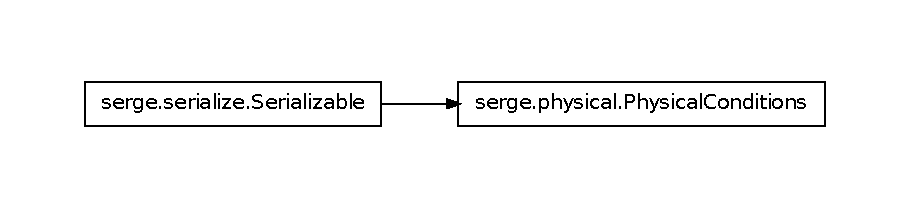
\includegraphics{inheritance-af60168d6ef2a0efccd77ed768d4695ea5a6a28a.pdf}
\index{PhysicalConditions (class in serge.physical)}

\begin{fulllineitems}
\phantomsection\label{physical:serge.physical.PhysicalConditions}\pysiglinewithargsret{\strong{class }\code{serge.physical.}\bfcode{PhysicalConditions}}{\emph{mass=0.0}, \emph{radius=0.0}, \emph{velocity=(0.0}, \emph{0.0)}, \emph{force=(0.0}, \emph{0.0)}, \emph{width=0.0}, \emph{height=0.0}, \emph{fixed=False}, \emph{friction=0.1}, \emph{elasticity=1.0}, \emph{group=0}, \emph{layers=-1}, \emph{update\_angle=False}, \emph{visual\_size=False}}{}
Bases: {\hyperref[common:serge.serialize.Serializable]{\code{serge.serialize.Serializable}}}

Represents physical parameters of an object

This includes the mass, velocity, force applied, acceleration
and the physical dimensions.
\index{init() (serge.physical.PhysicalConditions method)}

\begin{fulllineitems}
\phantomsection\label{physical:serge.physical.PhysicalConditions.init}\pysiglinewithargsret{\bfcode{init}}{}{}
Initialize from serialized form

\end{fulllineitems}

\index{setGeometry() (serge.physical.PhysicalConditions method)}

\begin{fulllineitems}
\phantomsection\label{physical:serge.physical.PhysicalConditions.setGeometry}\pysiglinewithargsret{\bfcode{setGeometry}}{\emph{radius=None}, \emph{width=None}, \emph{height=None}}{}
Set the geometry

You must specify either the radius or the width and height

\end{fulllineitems}

\index{updateFrom() (serge.physical.PhysicalConditions method)}

\begin{fulllineitems}
\phantomsection\label{physical:serge.physical.PhysicalConditions.updateFrom}\pysiglinewithargsret{\bfcode{updateFrom}}{\emph{physical\_conditions}}{}
Update the properties and our physics object

\end{fulllineitems}


\end{fulllineitems}



\section{PhysicalBody}
\label{physical:physicalbody}
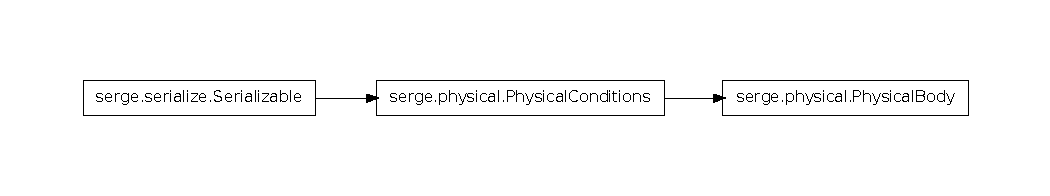
\includegraphics{inheritance-5faef0ba83f674f10cb10f70eb50925fd3f06318.pdf}
\index{PhysicalBody (class in serge.physical)}

\begin{fulllineitems}
\phantomsection\label{physical:serge.physical.PhysicalBody}\pysiglinewithargsret{\strong{class }\code{serge.physical.}\bfcode{PhysicalBody}}{\emph{mass}, \emph{**kw}}{}
Bases: {\hyperref[physical:serge.physical.PhysicalConditions]{\code{serge.physical.PhysicalConditions}}}

Physical conditions for an infinitesimal object

The object has no dimensions (shape) but still
has mass etc.

\end{fulllineitems}



\chapter{Events}
\label{events::doc}\label{events:events}\setbox0\vbox{
\begin{minipage}{0.95\linewidth}
\textbf{Contents}

\medskip

\begin{itemize}
\item {} 
{\hyperref[events:events]{Events}}
\begin{itemize}
\item {} 
{\hyperref[events:broadcaster]{Broadcaster}}

\item {} 
{\hyperref[events:geteventbroadcaster]{getEventBroadcaster}}

\item {} 
{\hyperref[events:id1]{Events}}

\end{itemize}

\end{itemize}
\end{minipage}}
\begin{center}\setlength{\fboxsep}{5pt}\shadowbox{\box0}\end{center}
\phantomsection\label{events:module-events}\index{events (module)}

\section{Broadcaster}
\label{events:broadcaster}\index{Broadcaster (class in serge.events)}

\begin{fulllineitems}
\phantomsection\label{events:serge.events.Broadcaster}\pysigline{\strong{class }\code{serge.events.}\bfcode{Broadcaster}}
Bases: {\hyperref[common:serge.common.EventAware]{\code{serge.common.EventAware}}}

The main event broadcaster

\end{fulllineitems}



\section{getEventBroadcaster}
\label{events:geteventbroadcaster}\index{getEventBroadcaster() (in module events)}

\begin{fulllineitems}
\phantomsection\label{events:events.getEventBroadcaster}\pysiglinewithargsret{\code{events.}\bfcode{getEventBroadcaster}}{}{}
Returns the global event broadcaster which is used for global level events

\end{fulllineitems}



\section{Events}
\label{events:id1}
Here are the global event definitions:

\begin{Verbatim}[commandchars=\\\{\}]
\PYG{c}{\PYGZsh{} Occurs when one object collides with another}
\PYG{n}{E\PYGZus{}COLLISION} \PYG{o}{=} \PYG{l+s}{'}\PYG{l+s}{collision}\PYG{l+s}{'}

\PYG{c}{\PYGZsh{} Mouse events related to the left mouse button}
\PYG{c}{\PYGZsh{}  - down is when the button is held down (fires continuously)}
\PYG{c}{\PYGZsh{}  - up is when the button is released}
\PYG{c}{\PYGZsh{}  - click is the mouse was down and then released}
\PYG{n}{E\PYGZus{}LEFT\PYGZus{}MOUSE\PYGZus{}DOWN} \PYG{o}{=} \PYG{l+s}{'}\PYG{l+s}{left-mouse-down}\PYG{l+s}{'}
\PYG{n}{E\PYGZus{}LEFT\PYGZus{}MOUSE\PYGZus{}UP} \PYG{o}{=} \PYG{l+s}{'}\PYG{l+s}{left-mouse-up}\PYG{l+s}{'}
\PYG{n}{E\PYGZus{}LEFT\PYGZus{}CLICK} \PYG{o}{=} \PYG{l+s}{'}\PYG{l+s}{left-click}\PYG{l+s}{'}

\PYG{c}{\PYGZsh{} Mouse events related to the right mouse button}
\PYG{c}{\PYGZsh{}  - down is when the button is held down (fires continuously)}
\PYG{c}{\PYGZsh{}  - up is when the button is released}
\PYG{c}{\PYGZsh{}  - click is the mouse was down and then released}
\PYG{n}{E\PYGZus{}RIGHT\PYGZus{}MOUSE\PYGZus{}DOWN} \PYG{o}{=} \PYG{l+s}{'}\PYG{l+s}{right-mouse-down}\PYG{l+s}{'}
\PYG{n}{E\PYGZus{}RIGHT\PYGZus{}MOUSE\PYGZus{}UP} \PYG{o}{=} \PYG{l+s}{'}\PYG{l+s}{right-mouse-up}\PYG{l+s}{'}
\PYG{n}{E\PYGZus{}RIGHT\PYGZus{}CLICK} \PYG{o}{=} \PYG{l+s}{'}\PYG{l+s}{right-click}\PYG{l+s}{'}

\PYG{c}{\PYGZsh{} Mouse events related to the wheel}
\PYG{c}{\PYGZsh{}  - wheel up the mouse wheel was moved up}
\PYG{c}{\PYGZsh{}  - wheel down the mouse wheel was moved down}
\PYG{n}{E\PYGZus{}MOUSE\PYGZus{}WHEEL\PYGZus{}UP} \PYG{o}{=} \PYG{l+s}{'}\PYG{l+s}{wheel-up-click}\PYG{l+s}{'}
\PYG{n}{E\PYGZus{}MOUSE\PYGZus{}WHEEL\PYGZus{}DOWN} \PYG{o}{=} \PYG{l+s}{'}\PYG{l+s}{wheel-down-click}\PYG{l+s}{'}

\PYG{c}{\PYGZsh{} Events related to actor and the world}
\PYG{n}{E\PYGZus{}ADDED\PYGZus{}TO\PYGZus{}WORLD} \PYG{o}{=} \PYG{l+s}{'}\PYG{l+s}{added-to-world}\PYG{l+s}{'}
\PYG{n}{E\PYGZus{}REMOVED\PYGZus{}FROM\PYGZus{}WORLD} \PYG{o}{=} \PYG{l+s}{'}\PYG{l+s}{remove-from-world}\PYG{l+s}{'}

\PYG{c}{\PYGZsh{} Events related to the world or layers}
\PYG{c}{\PYGZsh{}}
\PYG{c}{\PYGZsh{} The world is activated when it}
\PYG{c}{\PYGZsh{} becomes the current world for the engine.}
\PYG{c}{\PYGZsh{} The previously activated world is deactivated.}
\PYG{c}{\PYGZsh{}}
\PYG{c}{\PYGZsh{} Before and after render are triggered relative}
\PYG{c}{\PYGZsh{} to rendering the whole world or the layer}
\PYG{n}{E\PYGZus{}ACTIVATE\PYGZus{}WORLD} \PYG{o}{=} \PYG{l+s}{'}\PYG{l+s}{activate-world}\PYG{l+s}{'}
\PYG{n}{E\PYGZus{}DEACTIVATE\PYGZus{}WORLD} \PYG{o}{=} \PYG{l+s}{'}\PYG{l+s}{deactivate-world}\PYG{l+s}{'}
\PYG{n}{E\PYGZus{}BEFORE\PYGZus{}RENDER} \PYG{o}{=} \PYG{l+s}{'}\PYG{l+s}{before-render}\PYG{l+s}{'}
\PYG{n}{E\PYGZus{}AFTER\PYGZus{}RENDER} \PYG{o}{=} \PYG{l+s}{'}\PYG{l+s}{after-render}\PYG{l+s}{'}

\PYG{c}{\PYGZsh{} Events related to the keyboard}
\PYG{n}{E\PYGZus{}KEY\PYGZus{}DOWN} \PYG{o}{=} \PYG{l+s}{'}\PYG{l+s}{key-down}\PYG{l+s}{'}
\PYG{n}{E\PYGZus{}KEY\PYGZus{}UP} \PYG{o}{=} \PYG{l+s}{'}\PYG{l+s}{key-up}\PYG{l+s}{'}
\PYG{n}{E\PYGZus{}KEY\PYGZus{}CLICKED} \PYG{o}{=} \PYG{l+s}{'}\PYG{l+s}{key-clicked}\PYG{l+s}{'}

\PYG{c}{\PYGZsh{} Events related to the engine}
\PYG{n}{E\PYGZus{}BEFORE\PYGZus{}STOP} \PYG{o}{=} \PYG{l+s}{'}\PYG{l+s}{before-stop}\PYG{l+s}{'}  \PYG{c}{\PYGZsh{} The stop method has been called and the engine is about to quit}
\PYG{n}{E\PYGZus{}AFTER\PYGZus{}STOP} \PYG{o}{=} \PYG{l+s}{'}\PYG{l+s}{after-stop}\PYG{l+s}{'}  \PYG{c}{\PYGZsh{} The stop method has been called and the engine is quiting}

\PYG{c}{\PYGZsh{} Events related to movement}
\PYG{n}{E\PYGZus{}ACTOR\PYGZus{}ARRIVED} \PYG{o}{=} \PYG{l+s}{'}\PYG{l+s}{actor-arrived}\PYG{l+s}{'}

\PYG{c}{\PYGZsh{} Events related to sound and music}
\PYG{n}{E\PYGZus{}TRACK\PYGZus{}ENDED} \PYG{o}{=} \PYG{l+s}{'}\PYG{l+s}{track-ended}\PYG{l+s}{'}

\PYG{c}{\PYGZsh{} Drag and drop events}
\PYG{n}{E\PYGZus{}DRAG\PYGZus{}START} \PYG{o}{=} \PYG{l+s}{'}\PYG{l+s}{drag-start}\PYG{l+s}{'}
\PYG{n}{E\PYGZus{}DRAG\PYGZus{}ENDED} \PYG{o}{=} \PYG{l+s}{'}\PYG{l+s}{drag-ended}\PYG{l+s}{'}
\PYG{n}{E\PYGZus{}DROPPED\PYGZus{}ON} \PYG{o}{=} \PYG{l+s}{'}\PYG{l+s}{dropped-on}\PYG{l+s}{'}

\PYG{c}{\PYGZsh{} Events related to entering information}
\PYG{n}{E\PYGZus{}ACCEPT\PYGZus{}ENTRY} \PYG{o}{=} \PYG{l+s}{'}\PYG{l+s}{accept-entry}\PYG{l+s}{'}
\end{Verbatim}


\chapter{Geometry}
\label{geometry:geometry}\label{geometry::doc}\setbox0\vbox{
\begin{minipage}{0.95\linewidth}
\textbf{Contents}

\medskip

\begin{itemize}
\item {} 
{\hyperref[geometry:geometry]{Geometry}}
\begin{itemize}
\item {} 
{\hyperref[geometry:spatialobject]{SpatialObject}}

\item {} 
{\hyperref[geometry:rectangle]{Rectangle}}

\item {} 
{\hyperref[geometry:point]{Point}}

\item {} 
{\hyperref[geometry:simplerect]{SimpleRect}}

\item {} 
{\hyperref[geometry:vec2d]{Vec2d}}

\end{itemize}

\end{itemize}
\end{minipage}}
\begin{center}\setlength{\fboxsep}{5pt}\shadowbox{\box0}\end{center}
\phantomsection\label{geometry:module-events}\index{events (module)}

\section{SpatialObject}
\label{geometry:spatialobject}\index{SpatialObject (class in serge.geometry)}

\begin{fulllineitems}
\phantomsection\label{geometry:serge.geometry.SpatialObject}\pysigline{\strong{class }\code{serge.geometry.}\bfcode{SpatialObject}}
Bases: \code{object}

Represents a spatial object
\index{isInside() (serge.geometry.SpatialObject method)}

\begin{fulllineitems}
\phantomsection\label{geometry:serge.geometry.SpatialObject.isInside}\pysiglinewithargsret{\bfcode{isInside}}{\emph{other}}{}
Return True if this object is inside another

\end{fulllineitems}

\index{isOverlapping() (serge.geometry.SpatialObject method)}

\begin{fulllineitems}
\phantomsection\label{geometry:serge.geometry.SpatialObject.isOverlapping}\pysiglinewithargsret{\bfcode{isOverlapping}}{\emph{other}}{}
Return True if this object overlaps another

\end{fulllineitems}


\end{fulllineitems}



\section{Rectangle}
\label{geometry:rectangle}\index{Rectangle (class in serge.geometry)}

\begin{fulllineitems}
\phantomsection\label{geometry:serge.geometry.Rectangle}\pysiglinewithargsret{\strong{class }\code{serge.geometry.}\bfcode{Rectangle}}{\emph{x=0}, \emph{y=0}, \emph{w=0}, \emph{h=0}}{}
Bases: {\hyperref[geometry:serge.geometry.SpatialObject]{\code{serge.geometry.SpatialObject}}}, {\hyperref[common:serge.serialize.Serializable]{\code{serge.serialize.Serializable}}}

Represents a rectangle
\index{fromCenter() (serge.geometry.Rectangle class method)}

\begin{fulllineitems}
\phantomsection\label{geometry:serge.geometry.Rectangle.fromCenter}\pysiglinewithargsret{\strong{classmethod }\bfcode{fromCenter}}{\emph{cx}, \emph{cy}, \emph{w}, \emph{h}}{}
Return a new rectangle giving the center x, y and width, height

\end{fulllineitems}

\index{getArea() (serge.geometry.Rectangle method)}

\begin{fulllineitems}
\phantomsection\label{geometry:serge.geometry.Rectangle.getArea}\pysiglinewithargsret{\bfcode{getArea}}{}{}
Return the area of the shape

\end{fulllineitems}

\index{getDistanceFrom() (serge.geometry.Rectangle method)}

\begin{fulllineitems}
\phantomsection\label{geometry:serge.geometry.Rectangle.getDistanceFrom}\pysiglinewithargsret{\bfcode{getDistanceFrom}}{\emph{other}}{}
Return the distance we are from another

\end{fulllineitems}

\index{getOrigin() (serge.geometry.Rectangle method)}

\begin{fulllineitems}
\phantomsection\label{geometry:serge.geometry.Rectangle.getOrigin}\pysiglinewithargsret{\bfcode{getOrigin}}{}{}
Get the left and top coords

\end{fulllineitems}

\index{getRelativeLocation() (serge.geometry.Rectangle method)}

\begin{fulllineitems}
\phantomsection\label{geometry:serge.geometry.Rectangle.getRelativeLocation}\pysiglinewithargsret{\bfcode{getRelativeLocation}}{\emph{other}}{}
Return the relative location of another object

\end{fulllineitems}

\index{getRelativeLocationCentered() (serge.geometry.Rectangle method)}

\begin{fulllineitems}
\phantomsection\label{geometry:serge.geometry.Rectangle.getRelativeLocationCentered}\pysiglinewithargsret{\bfcode{getRelativeLocationCentered}}{\emph{other}}{}
Return the relative location of another object

\end{fulllineitems}

\index{getSpatial() (serge.geometry.Rectangle method)}

\begin{fulllineitems}
\phantomsection\label{geometry:serge.geometry.Rectangle.getSpatial}\pysiglinewithargsret{\bfcode{getSpatial}}{}{}
Return spatial details

\end{fulllineitems}

\index{getSpatialCentered() (serge.geometry.Rectangle method)}

\begin{fulllineitems}
\phantomsection\label{geometry:serge.geometry.Rectangle.getSpatialCentered}\pysiglinewithargsret{\bfcode{getSpatialCentered}}{}{}
Return spatial details

\end{fulllineitems}

\index{init() (serge.geometry.Rectangle method)}

\begin{fulllineitems}
\phantomsection\label{geometry:serge.geometry.Rectangle.init}\pysiglinewithargsret{\bfcode{init}}{}{}
Initialize from serialized

\end{fulllineitems}

\index{isInside() (serge.geometry.Rectangle method)}

\begin{fulllineitems}
\phantomsection\label{geometry:serge.geometry.Rectangle.isInside}\pysiglinewithargsret{\bfcode{isInside}}{\emph{other}}{}
Return True if this object is inside another

\end{fulllineitems}

\index{isOverlapping() (serge.geometry.Rectangle method)}

\begin{fulllineitems}
\phantomsection\label{geometry:serge.geometry.Rectangle.isOverlapping}\pysiglinewithargsret{\bfcode{isOverlapping}}{\emph{other}}{}
Return True if this object overlaps another

\end{fulllineitems}

\index{move() (serge.geometry.Rectangle method)}

\begin{fulllineitems}
\phantomsection\label{geometry:serge.geometry.Rectangle.move}\pysiglinewithargsret{\bfcode{move}}{\emph{dx}, \emph{dy}}{}
Move the actor

\end{fulllineitems}

\index{moveTo() (serge.geometry.Rectangle method)}

\begin{fulllineitems}
\phantomsection\label{geometry:serge.geometry.Rectangle.moveTo}\pysiglinewithargsret{\bfcode{moveTo}}{\emph{x}, \emph{y}, \emph{override\_lock=False}}{}
Move the center of this object to the given location, unless it is locked

This is the main method used to implement the position of the 
shape. This is the one to override.

\end{fulllineitems}

\index{resizeBy() (serge.geometry.Rectangle method)}

\begin{fulllineitems}
\phantomsection\label{geometry:serge.geometry.Rectangle.resizeBy}\pysiglinewithargsret{\bfcode{resizeBy}}{\emph{w}, \emph{h}}{}
Resize the spatial by the given extent

\end{fulllineitems}

\index{resizeTo() (serge.geometry.Rectangle method)}

\begin{fulllineitems}
\phantomsection\label{geometry:serge.geometry.Rectangle.resizeTo}\pysiglinewithargsret{\bfcode{resizeTo}}{\emph{w}, \emph{h}}{}
Resize the spatial by the given extent

\end{fulllineitems}

\index{scale() (serge.geometry.Rectangle method)}

\begin{fulllineitems}
\phantomsection\label{geometry:serge.geometry.Rectangle.scale}\pysiglinewithargsret{\bfcode{scale}}{\emph{factor}}{}
Rescale the spatial extent

\end{fulllineitems}

\index{setOrigin() (serge.geometry.Rectangle method)}

\begin{fulllineitems}
\phantomsection\label{geometry:serge.geometry.Rectangle.setOrigin}\pysiglinewithargsret{\bfcode{setOrigin}}{\emph{x}, \emph{y}}{}
Set the left and top coords

\end{fulllineitems}

\index{setSpatial() (serge.geometry.Rectangle method)}

\begin{fulllineitems}
\phantomsection\label{geometry:serge.geometry.Rectangle.setSpatial}\pysiglinewithargsret{\bfcode{setSpatial}}{\emph{x}, \emph{y}, \emph{w}, \emph{h}}{}
Set the spatial details of ourself

\end{fulllineitems}

\index{setSpatialCentered() (serge.geometry.Rectangle method)}

\begin{fulllineitems}
\phantomsection\label{geometry:serge.geometry.Rectangle.setSpatialCentered}\pysiglinewithargsret{\bfcode{setSpatialCentered}}{\emph{x}, \emph{y}, \emph{w}, \emph{h}}{}
Set the spatial details of ourself

\end{fulllineitems}


\end{fulllineitems}



\section{Point}
\label{geometry:point}\index{Point (class in serge.geometry)}

\begin{fulllineitems}
\phantomsection\label{geometry:serge.geometry.Point}\pysiglinewithargsret{\strong{class }\code{serge.geometry.}\bfcode{Point}}{\emph{x}, \emph{y}}{}
Bases: {\hyperref[geometry:serge.geometry.Rectangle]{\code{serge.geometry.Rectangle}}}

Represents a point
\index{isInside() (serge.geometry.Point method)}

\begin{fulllineitems}
\phantomsection\label{geometry:serge.geometry.Point.isInside}\pysiglinewithargsret{\bfcode{isInside}}{\emph{other}}{}
Return True if this object is inside another

\end{fulllineitems}

\index{isOverlapping() (serge.geometry.Point method)}

\begin{fulllineitems}
\phantomsection\label{geometry:serge.geometry.Point.isOverlapping}\pysiglinewithargsret{\bfcode{isOverlapping}}{\emph{other}}{}
Return True if this object overlaps another

\end{fulllineitems}


\end{fulllineitems}



\section{SimpleRect}
\label{geometry:simplerect}\index{SimpleRect (class in serge.geometry)}

\begin{fulllineitems}
\phantomsection\label{geometry:serge.geometry.SimpleRect}\pysiglinewithargsret{\strong{class }\code{serge.geometry.}\bfcode{SimpleRect}}{\emph{*args}}{}
Bases: \code{list}

A simple rectangle implementation
\index{collidepoint() (serge.geometry.SimpleRect method)}

\begin{fulllineitems}
\phantomsection\label{geometry:serge.geometry.SimpleRect.collidepoint}\pysiglinewithargsret{\bfcode{collidepoint}}{\emph{x}, \emph{y}}{}
Return True if this rectangle collides with another

\end{fulllineitems}

\index{colliderect() (serge.geometry.SimpleRect method)}

\begin{fulllineitems}
\phantomsection\label{geometry:serge.geometry.SimpleRect.colliderect}\pysiglinewithargsret{\bfcode{colliderect}}{\emph{other}}{}
Return True if this rectangle collides with another

\end{fulllineitems}

\index{contains() (serge.geometry.SimpleRect method)}

\begin{fulllineitems}
\phantomsection\label{geometry:serge.geometry.SimpleRect.contains}\pysiglinewithargsret{\bfcode{contains}}{\emph{other}}{}
Return True if this rectangle contains another

\end{fulllineitems}

\index{inflate() (serge.geometry.SimpleRect method)}

\begin{fulllineitems}
\phantomsection\label{geometry:serge.geometry.SimpleRect.inflate}\pysiglinewithargsret{\bfcode{inflate}}{\emph{w}, \emph{h}}{}
Inflate to new width and height staying in the same centered place

\end{fulllineitems}

\index{inflate\_ip() (serge.geometry.SimpleRect method)}

\begin{fulllineitems}
\phantomsection\label{geometry:serge.geometry.SimpleRect.inflate_ip}\pysiglinewithargsret{\bfcode{inflate\_ip}}{\emph{w}, \emph{h}}{}
Inflate current rectangle to new width and height staying in the same centered place

\end{fulllineitems}

\index{move\_ip() (serge.geometry.SimpleRect method)}

\begin{fulllineitems}
\phantomsection\label{geometry:serge.geometry.SimpleRect.move_ip}\pysiglinewithargsret{\bfcode{move\_ip}}{\emph{dx}, \emph{dy}}{}
Move in place

\end{fulllineitems}


\end{fulllineitems}

\phantomsection\label{geometry:module-simplevecs}\index{simplevecs (module)}

\section{Vec2d}
\label{geometry:vec2d}\index{Vec2d (class in serge.simplevecs)}

\begin{fulllineitems}
\phantomsection\label{geometry:serge.simplevecs.Vec2d}\pysiglinewithargsret{\strong{class }\code{serge.simplevecs.}\bfcode{Vec2d}}{\emph{x\_or\_pair=None}, \emph{y=None}}{}
Bases: \code{object}

2d vector class, supports vector and scalar operators,
and also provides some high level functions
\index{angle (serge.simplevecs.Vec2d attribute)}

\begin{fulllineitems}
\phantomsection\label{geometry:serge.simplevecs.Vec2d.angle}\pysigline{\bfcode{angle}}
Gets or sets the angle (in radians) of a vector

\end{fulllineitems}

\index{angle\_degrees (serge.simplevecs.Vec2d attribute)}

\begin{fulllineitems}
\phantomsection\label{geometry:serge.simplevecs.Vec2d.angle_degrees}\pysigline{\bfcode{angle\_degrees}}
Gets or sets the angle (in degrees) of a vector

\end{fulllineitems}

\index{cpvrotate() (serge.simplevecs.Vec2d method)}

\begin{fulllineitems}
\phantomsection\label{geometry:serge.simplevecs.Vec2d.cpvrotate}\pysiglinewithargsret{\bfcode{cpvrotate}}{\emph{other}}{}
Uses complex multiplication to rotate this vector by the other.

\end{fulllineitems}

\index{cpvunrotate() (serge.simplevecs.Vec2d method)}

\begin{fulllineitems}
\phantomsection\label{geometry:serge.simplevecs.Vec2d.cpvunrotate}\pysiglinewithargsret{\bfcode{cpvunrotate}}{\emph{other}}{}
The inverse of cpvrotate

\end{fulllineitems}

\index{cross() (serge.simplevecs.Vec2d method)}

\begin{fulllineitems}
\phantomsection\label{geometry:serge.simplevecs.Vec2d.cross}\pysiglinewithargsret{\bfcode{cross}}{\emph{other}}{}
The cross product between the vector and other vector
v1.cross(v2) -\textgreater{} v1.x*v2.y - v2.y*v1.x
\begin{quote}\begin{description}
\item[{Returns}] \leavevmode
The cross product

\end{description}\end{quote}

\end{fulllineitems}

\index{dot() (serge.simplevecs.Vec2d method)}

\begin{fulllineitems}
\phantomsection\label{geometry:serge.simplevecs.Vec2d.dot}\pysiglinewithargsret{\bfcode{dot}}{\emph{other}}{}
The dot product between the vector and other vector
v1.dot(v2) -\textgreater{} v1.x*v2.x + v1.y*v2.y
\begin{quote}\begin{description}
\item[{Returns}] \leavevmode
The dot product

\end{description}\end{quote}

\end{fulllineitems}

\index{from\_param() (serge.simplevecs.Vec2d class method)}

\begin{fulllineitems}
\phantomsection\label{geometry:serge.simplevecs.Vec2d.from_param}\pysiglinewithargsret{\strong{classmethod }\bfcode{from\_param}}{\emph{arg}}{}
Used by ctypes to automatically create Vec2ds

\end{fulllineitems}

\index{get\_angle\_between() (serge.simplevecs.Vec2d method)}

\begin{fulllineitems}
\phantomsection\label{geometry:serge.simplevecs.Vec2d.get_angle_between}\pysiglinewithargsret{\bfcode{get\_angle\_between}}{\emph{other}}{}
Get the angle between the vector and the other in radians
\begin{quote}\begin{description}
\item[{Returns}] \leavevmode
The angle

\end{description}\end{quote}

\end{fulllineitems}

\index{get\_angle\_degrees\_between() (serge.simplevecs.Vec2d method)}

\begin{fulllineitems}
\phantomsection\label{geometry:serge.simplevecs.Vec2d.get_angle_degrees_between}\pysiglinewithargsret{\bfcode{get\_angle\_degrees\_between}}{\emph{other}}{}
Get the angle between the vector and the other in degrees
\begin{quote}\begin{description}
\item[{Returns}] \leavevmode
The angle (in degrees)

\end{description}\end{quote}

\end{fulllineitems}

\index{get\_dist\_sqrd() (serge.simplevecs.Vec2d method)}

\begin{fulllineitems}
\phantomsection\label{geometry:serge.simplevecs.Vec2d.get_dist_sqrd}\pysiglinewithargsret{\bfcode{get\_dist\_sqrd}}{\emph{other}}{}
The squared distance between the vector and other vector
It is more efficent to use this method than to call get\_distance()
first and then do a sqrt() on the result.
\begin{quote}\begin{description}
\item[{Returns}] \leavevmode
The squared distance

\end{description}\end{quote}

\end{fulllineitems}

\index{get\_distance() (serge.simplevecs.Vec2d method)}

\begin{fulllineitems}
\phantomsection\label{geometry:serge.simplevecs.Vec2d.get_distance}\pysiglinewithargsret{\bfcode{get\_distance}}{\emph{other}}{}
The distance between the vector and other vector
\begin{quote}\begin{description}
\item[{Returns}] \leavevmode
The distance

\end{description}\end{quote}

\end{fulllineitems}

\index{get\_length() (serge.simplevecs.Vec2d method)}

\begin{fulllineitems}
\phantomsection\label{geometry:serge.simplevecs.Vec2d.get_length}\pysiglinewithargsret{\bfcode{get\_length}}{}{}
Get the length of the vector.
\begin{quote}\begin{description}
\item[{Returns}] \leavevmode
The length

\end{description}\end{quote}

\end{fulllineitems}

\index{get\_length\_sqrd() (serge.simplevecs.Vec2d method)}

\begin{fulllineitems}
\phantomsection\label{geometry:serge.simplevecs.Vec2d.get_length_sqrd}\pysiglinewithargsret{\bfcode{get\_length\_sqrd}}{}{}
Get the squared length of the vector.
It is more efficent to use this method instead of first call 
get\_length() or access .length and then do a sqrt().
\begin{quote}\begin{description}
\item[{Returns}] \leavevmode
The squared length

\end{description}\end{quote}

\end{fulllineitems}

\index{int\_tuple (serge.simplevecs.Vec2d attribute)}

\begin{fulllineitems}
\phantomsection\label{geometry:serge.simplevecs.Vec2d.int_tuple}\pysigline{\bfcode{int\_tuple}}
Return the x and y values of this vector as ints

\end{fulllineitems}

\index{length (serge.simplevecs.Vec2d attribute)}

\begin{fulllineitems}
\phantomsection\label{geometry:serge.simplevecs.Vec2d.length}\pysigline{\bfcode{length}}
Gets or sets the magnitude of the vector

\end{fulllineitems}

\index{normalize\_return\_length() (serge.simplevecs.Vec2d method)}

\begin{fulllineitems}
\phantomsection\label{geometry:serge.simplevecs.Vec2d.normalize_return_length}\pysiglinewithargsret{\bfcode{normalize\_return\_length}}{}{}
Normalize the vector and return its length before the normalization
\begin{quote}\begin{description}
\item[{Returns}] \leavevmode
The length before the normalization

\end{description}\end{quote}

\end{fulllineitems}

\index{normalized() (serge.simplevecs.Vec2d method)}

\begin{fulllineitems}
\phantomsection\label{geometry:serge.simplevecs.Vec2d.normalized}\pysiglinewithargsret{\bfcode{normalized}}{}{}
Get a normalized copy of the vector
Note: This function will return 0 if the length of the vector is 0.
\begin{quote}\begin{description}
\item[{Returns}] \leavevmode
A normalized vector

\end{description}\end{quote}

\end{fulllineitems}

\index{ones() (serge.simplevecs.Vec2d static method)}

\begin{fulllineitems}
\phantomsection\label{geometry:serge.simplevecs.Vec2d.ones}\pysiglinewithargsret{\strong{static }\bfcode{ones}}{}{}
A vector where both x and y is 1

\end{fulllineitems}

\index{rotate() (serge.simplevecs.Vec2d method)}

\begin{fulllineitems}
\phantomsection\label{geometry:serge.simplevecs.Vec2d.rotate}\pysiglinewithargsret{\bfcode{rotate}}{\emph{angle\_radians}}{}
Rotate the vector by angle\_radians radians.

\end{fulllineitems}

\index{rotate\_degrees() (serge.simplevecs.Vec2d method)}

\begin{fulllineitems}
\phantomsection\label{geometry:serge.simplevecs.Vec2d.rotate_degrees}\pysiglinewithargsret{\bfcode{rotate\_degrees}}{\emph{angle\_degrees}}{}
Rotate the vector by angle\_degrees degrees.

\end{fulllineitems}

\index{rotated() (serge.simplevecs.Vec2d method)}

\begin{fulllineitems}
\phantomsection\label{geometry:serge.simplevecs.Vec2d.rotated}\pysiglinewithargsret{\bfcode{rotated}}{\emph{angle\_radians}}{}
Create and return a new vector by rotating this vector by 
angle\_radians radians.
\begin{quote}\begin{description}
\item[{Returns}] \leavevmode
Rotade vector

\end{description}\end{quote}

\end{fulllineitems}

\index{rotated\_degrees() (serge.simplevecs.Vec2d method)}

\begin{fulllineitems}
\phantomsection\label{geometry:serge.simplevecs.Vec2d.rotated_degrees}\pysiglinewithargsret{\bfcode{rotated\_degrees}}{\emph{angle\_degrees}}{}
Create and return a new vector by rotating this vector by 
angle\_degrees degrees.
\begin{quote}\begin{description}
\item[{Returns}] \leavevmode
Rotade vector

\end{description}\end{quote}

\end{fulllineitems}

\index{unit() (serge.simplevecs.Vec2d static method)}

\begin{fulllineitems}
\phantomsection\label{geometry:serge.simplevecs.Vec2d.unit}\pysiglinewithargsret{\strong{static }\bfcode{unit}}{}{}
A unit vector pointing up

\end{fulllineitems}

\index{zero() (serge.simplevecs.Vec2d static method)}

\begin{fulllineitems}
\phantomsection\label{geometry:serge.simplevecs.Vec2d.zero}\pysiglinewithargsret{\strong{static }\bfcode{zero}}{}{}
A vector of zero length

\end{fulllineitems}


\end{fulllineitems}



\chapter{Common}
\label{common::doc}\label{common:common}\setbox0\vbox{
\begin{minipage}{0.95\linewidth}
\textbf{Contents}

\medskip

\begin{itemize}
\item {} 
{\hyperref[common:common]{Common}}
\begin{itemize}
\item {} 
{\hyperref[common:loggable]{Loggable}}

\item {} 
{\hyperref[common:getlogger]{getLogger}}

\item {} 
{\hyperref[common:eventaware]{EventAware}}

\item {} 
{\hyperref[common:serializable]{Serializable}}

\item {} 
{\hyperref[common:generalstore]{GeneralStore}}

\end{itemize}

\end{itemize}
\end{minipage}}
\begin{center}\setlength{\fboxsep}{5pt}\shadowbox{\box0}\end{center}
\phantomsection\label{common:module-common}\index{common (module)}\phantomsection\label{common:module-registry}\index{registry (module)}

\section{Loggable}
\label{common:loggable}\index{Loggable (class in serge.common)}

\begin{fulllineitems}
\phantomsection\label{common:serge.common.Loggable}\pysigline{\strong{class }\code{serge.common.}\bfcode{Loggable}}
Bases: \code{object}

A helper class that adds a logger to a class

Each instance of the class will have a \emph{log} attribute and can
use this to log output. The \emph{log} attrbute is a logger with the
usual \emph{debug}, \emph{warn}, \emph{info}, and \emph{error} methods.
\index{addLogger() (serge.common.Loggable method)}

\begin{fulllineitems}
\phantomsection\label{common:serge.common.Loggable.addLogger}\pysiglinewithargsret{\bfcode{addLogger}}{}{}
Add a logger

\end{fulllineitems}


\end{fulllineitems}



\section{getLogger}
\label{common:getlogger}\index{getLogger() (in module registry)}

\begin{fulllineitems}
\phantomsection\label{common:registry.getLogger}\pysiglinewithargsret{\code{registry.}\bfcode{getLogger}}{\emph{name}}{}
Return a named logger - mainly used when logging from a non-loggable object

\end{fulllineitems}



\section{EventAware}
\label{common:eventaware}\index{EventAware (class in serge.common)}

\begin{fulllineitems}
\phantomsection\label{common:serge.common.EventAware}\pysigline{\strong{class }\code{serge.common.}\bfcode{EventAware}}
Bases: \code{object}

A mixin class that allows objects to respond to events
\index{handleEvent() (serge.common.EventAware method)}

\begin{fulllineitems}
\phantomsection\label{common:serge.common.EventAware.handleEvent}\pysiglinewithargsret{\bfcode{handleEvent}}{\emph{event}}{}
Handle an incoming event

\end{fulllineitems}

\index{initEvents() (serge.common.EventAware method)}

\begin{fulllineitems}
\phantomsection\label{common:serge.common.EventAware.initEvents}\pysiglinewithargsret{\bfcode{initEvents}}{}{}
Initialise the events system

\end{fulllineitems}

\index{linkEvent() (serge.common.EventAware method)}

\begin{fulllineitems}
\phantomsection\label{common:serge.common.EventAware.linkEvent}\pysiglinewithargsret{\bfcode{linkEvent}}{\emph{name}, \emph{callback}, \emph{arg=None}}{}
Link an event to a callback

\end{fulllineitems}

\index{processEvent() (serge.common.EventAware method)}

\begin{fulllineitems}
\phantomsection\label{common:serge.common.EventAware.processEvent}\pysiglinewithargsret{\bfcode{processEvent}}{\emph{event}}{}
Process an incoming event

\end{fulllineitems}

\index{registerEvent() (serge.common.EventAware method)}

\begin{fulllineitems}
\phantomsection\label{common:serge.common.EventAware.registerEvent}\pysiglinewithargsret{\bfcode{registerEvent}}{\emph{event}}{}
Register an event

\end{fulllineitems}

\index{registerEvents() (serge.common.EventAware method)}

\begin{fulllineitems}
\phantomsection\label{common:serge.common.EventAware.registerEvents}\pysiglinewithargsret{\bfcode{registerEvents}}{\emph{events}}{}
Register a number of events

\end{fulllineitems}

\index{registerEventsFromModule() (serge.common.EventAware method)}

\begin{fulllineitems}
\phantomsection\label{common:serge.common.EventAware.registerEventsFromModule}\pysiglinewithargsret{\bfcode{registerEventsFromModule}}{\emph{module}}{}
Register all events found in the module

Events must be strings and their name must be of the 
form E\_THE\_NAME

ie: Begins with an `E' and is all uppercase

\end{fulllineitems}

\index{unlinkEvent() (serge.common.EventAware method)}

\begin{fulllineitems}
\phantomsection\label{common:serge.common.EventAware.unlinkEvent}\pysiglinewithargsret{\bfcode{unlinkEvent}}{\emph{name}, \emph{callback=None}}{}
Unlink an event from a callback

\end{fulllineitems}


\end{fulllineitems}



\section{Serializable}
\label{common:serializable}\index{Serializable (class in serge.serialize)}

\begin{fulllineitems}
\phantomsection\label{common:serge.serialize.Serializable}\pysigline{\strong{class }\code{serge.serialize.}\bfcode{Serializable}}
Bases: \code{object}

A mixing class to help serialize and deserialize objects
\index{asString() (serge.serialize.Serializable method)}

\begin{fulllineitems}
\phantomsection\label{common:serge.serialize.Serializable.asString}\pysiglinewithargsret{\bfcode{asString}}{}{}
Return the properties of this object as a string

\end{fulllineitems}

\index{copy() (serge.serialize.Serializable method)}

\begin{fulllineitems}
\phantomsection\label{common:serge.serialize.Serializable.copy}\pysiglinewithargsret{\bfcode{copy}}{}{}
Return another copy of this item

\end{fulllineitems}

\index{createInstance() (serge.serialize.Serializable class method)}

\begin{fulllineitems}
\phantomsection\label{common:serge.serialize.Serializable.createInstance}\pysiglinewithargsret{\strong{classmethod }\bfcode{createInstance}}{}{}
Return an instance of the class with all default properties set

\end{fulllineitems}

\index{fromFile() (serge.serialize.Serializable class method)}

\begin{fulllineitems}
\phantomsection\label{common:serge.serialize.Serializable.fromFile}\pysiglinewithargsret{\strong{classmethod }\bfcode{fromFile}}{\emph{filename}}{}
Return a new instance from a file

\end{fulllineitems}

\index{fromString() (serge.serialize.Serializable class method)}

\begin{fulllineitems}
\phantomsection\label{common:serge.serialize.Serializable.fromString}\pysiglinewithargsret{\strong{classmethod }\bfcode{fromString}}{\emph{text}}{}
Return a new instance from a string

\end{fulllineitems}

\index{init() (serge.serialize.Serializable method)}

\begin{fulllineitems}
\phantomsection\label{common:serge.serialize.Serializable.init}\pysiglinewithargsret{\bfcode{init}}{}{}
Implement this method to do any object initialization after unpickling

\end{fulllineitems}

\index{toFile() (serge.serialize.Serializable method)}

\begin{fulllineitems}
\phantomsection\label{common:serge.serialize.Serializable.toFile}\pysiglinewithargsret{\bfcode{toFile}}{\emph{filename}}{}
Store this object in a file

\end{fulllineitems}


\end{fulllineitems}



\section{GeneralStore}
\label{common:generalstore}\index{GeneralStore (class in serge.registry)}

\begin{fulllineitems}
\phantomsection\label{common:serge.registry.GeneralStore}\pysigline{\strong{class }\code{serge.registry.}\bfcode{GeneralStore}}
Bases: {\hyperref[common:serge.serialize.Serializable]{\code{serge.serialize.Serializable}}}

Stores things
\index{clearItems() (serge.registry.GeneralStore method)}

\begin{fulllineitems}
\phantomsection\label{common:serge.registry.GeneralStore.clearItems}\pysiglinewithargsret{\bfcode{clearItems}}{}{}
Clear all the items

\end{fulllineitems}

\index{duplicateItem() (serge.registry.GeneralStore method)}

\begin{fulllineitems}
\phantomsection\label{common:serge.registry.GeneralStore.duplicateItem}\pysiglinewithargsret{\bfcode{duplicateItem}}{\emph{name}, \emph{new\_name}}{}
Create a duplicate of the named item with a new name

\end{fulllineitems}

\index{getItem() (serge.registry.GeneralStore method)}

\begin{fulllineitems}
\phantomsection\label{common:serge.registry.GeneralStore.getItem}\pysiglinewithargsret{\bfcode{getItem}}{\emph{name}}{}
Return an item

\end{fulllineitems}

\index{getItemDefinitions() (serge.registry.GeneralStore method)}

\begin{fulllineitems}
\phantomsection\label{common:serge.registry.GeneralStore.getItemDefinitions}\pysiglinewithargsret{\bfcode{getItemDefinitions}}{}{}
Return all the item definitions

\end{fulllineitems}

\index{getItems() (serge.registry.GeneralStore method)}

\begin{fulllineitems}
\phantomsection\label{common:serge.registry.GeneralStore.getItems}\pysiglinewithargsret{\bfcode{getItems}}{}{}
Return all the items

\end{fulllineitems}

\index{getNames() (serge.registry.GeneralStore method)}

\begin{fulllineitems}
\phantomsection\label{common:serge.registry.GeneralStore.getNames}\pysiglinewithargsret{\bfcode{getNames}}{}{}
Return the names of all the items

\end{fulllineitems}

\index{init() (serge.registry.GeneralStore method)}

\begin{fulllineitems}
\phantomsection\label{common:serge.registry.GeneralStore.init}\pysiglinewithargsret{\bfcode{init}}{}{}
Initialise from serialized form

\end{fulllineitems}

\index{registerItem() (serge.registry.GeneralStore method)}

\begin{fulllineitems}
\phantomsection\label{common:serge.registry.GeneralStore.registerItem}\pysiglinewithargsret{\bfcode{registerItem}}{\emph{name}, \emph{*args}, \emph{**kw}}{}
Register an item

\end{fulllineitems}

\index{removeItem() (serge.registry.GeneralStore method)}

\begin{fulllineitems}
\phantomsection\label{common:serge.registry.GeneralStore.removeItem}\pysiglinewithargsret{\bfcode{removeItem}}{\emph{name}}{}
Remove the named item

\end{fulllineitems}

\index{setPath() (serge.registry.GeneralStore method)}

\begin{fulllineitems}
\phantomsection\label{common:serge.registry.GeneralStore.setPath}\pysiglinewithargsret{\bfcode{setPath}}{\emph{path}}{}
Set our base path to locate images

\end{fulllineitems}


\end{fulllineitems}



\chapter{Indices and tables}
\label{index:indices-and-tables}\begin{itemize}
\item {} 
\emph{genindex}

\item {} 
\emph{modindex}

\item {} 
\emph{search}

\end{itemize}


\renewcommand{\indexname}{Python Module Index}
\begin{theindex}
\def\bigletter#1{{\Large\sffamily#1}\nopagebreak\vspace{1mm}}
\bigletter{a}
\item {\texttt{actor}}, \pageref{actor:module-actor}
\indexspace
\bigletter{c}
\item {\texttt{camera}}, \pageref{renderering:module-camera}
\item {\texttt{common}}, \pageref{common:module-common}
\indexspace
\bigletter{e}
\item {\texttt{engine}}, \pageref{engine:module-engine}
\item {\texttt{events}}, \pageref{input:module-events}
\indexspace
\bigletter{p}
\item {\texttt{physical}}, \pageref{physical:module-physical}
\indexspace
\bigletter{r}
\item {\texttt{registry}}, \pageref{common:module-registry}
\item {\texttt{render}}, \pageref{renderering:module-render}
\indexspace
\bigletter{s}
\item {\texttt{serge.blocks.achievements}}, \pageref{blocks:module-serge.blocks.achievements}
\item {\texttt{serge.blocks.actors}}, \pageref{blocks:module-serge.blocks.actors}
\item {\texttt{serge.blocks.behaviours}}, \pageref{blocks:module-serge.blocks.behaviours}
\item {\texttt{serge.blocks.conversation}}, \pageref{blocks:module-serge.blocks.conversation}
\item {\texttt{serge.blocks.directions}}, \pageref{blocks:module-serge.blocks.directions}
\item {\texttt{serge.blocks.dragndrop}}, \pageref{blocks:module-serge.blocks.dragndrop}
\item {\texttt{serge.blocks.effects}}, \pageref{blocks:module-serge.blocks.effects}
\item {\texttt{serge.blocks.fractals}}, \pageref{blocks:module-serge.blocks.fractals}
\item {\texttt{serge.blocks.layout}}, \pageref{blocks:module-serge.blocks.layout}
\item {\texttt{serge.blocks.scores}}, \pageref{blocks:module-serge.blocks.scores}
\item {\texttt{serge.blocks.singletons}}, \pageref{blocks:module-serge.blocks.singletons}
\item {\texttt{serge.blocks.themes}}, \pageref{blocks:module-serge.blocks.themes}
\item {\texttt{serge.blocks.tiled}}, \pageref{blocks:module-serge.blocks.tiled}
\item {\texttt{serge.blocks.utils}}, \pageref{blocks:module-serge.blocks.utils}
\item {\texttt{serge.blocks.visualblocks}}, \pageref{blocks:module-serge.blocks.visualblocks}
\item {\texttt{serge.blocks.visualeffects}}, \pageref{blocks:module-serge.blocks.visualeffects}
\item {\texttt{serge.blocks.worker}}, \pageref{blocks:module-serge.blocks.worker}
\item {\texttt{simplevecs}}, \pageref{geometry:module-simplevecs}
\item {\texttt{sound}}, \pageref{sound:module-sound}
\indexspace
\bigletter{v}
\item {\texttt{visual}}, \pageref{visual:module-visual}
\indexspace
\bigletter{w}
\item {\texttt{world}}, \pageref{world:module-world}
\indexspace
\bigletter{z}
\item {\texttt{zone}}, \pageref{zone:module-zone}
\end{theindex}

\renewcommand{\indexname}{Index}
\printindex
\end{document}
